\documentclass[11pt,a4paper]{extreport}
\usepackage[a4paper, top=20mm, bottom=20mm, left=25mm, right=20mm]{geometry}
\usepackage[utf8]{inputenc}
\usepackage[T1,T5]{fontenc}
\usepackage[vietnamese,english]{babel}
\DeclareUnicodeCharacter{0105}{{\fontencoding{T1}\selectfont\k{a}}}
\usepackage{mathptmx}
\usepackage{cite}

\usepackage{indentfirst}
\usepackage{parskip}
\setlength{\parskip}{6pt}
\setlength{\parindent}{1cm}
\linespread{1.2}

\usepackage{enumitem}
\setlist[itemize]{label=--, leftmargin=1.5cm}

\clubpenalty=10000
\widowpenalty=10000
\displaywidowpenalty=10000

\usepackage{amsmath}
\usepackage{amssymb}
\usepackage{booktabs}
\usepackage{array}
\newcolumntype{C}[1]{>{\centering\arraybackslash}p{#1}}
\usepackage{tabularx}
\usepackage{longtable}
\usepackage{pdflscape}
\usepackage{graphicx}
\usepackage{tikz}
\usetikzlibrary{positioning,arrows.meta}
\usepackage[font=small, labelfont=bf, textfont=bf, justification=centering]{caption}
\usepackage{subcaption}
\usepackage{multirow}
\usepackage{float}
\usepackage[table]{xcolor}
\usepackage{titlesec}
\usepackage{fancyhdr}
\usepackage[hidelinks,hypertexnames=false]{hyperref}

\newcommand{\ghrepo}{https://github.com/pqui-345/BiGCN-Plus-Rumor-Detection/blob/main}
\newcommand{\coderef}[2]{\textnormal{[\href{\ghrepo/#1}{#2}]}}

% Định dạng tiêu đề chương và mục theo đúng chuẩn main.tex của tác giả
\titleformat{\chapter}[display]
  {\normalfont\bfseries\centering}
  {\fontsize{16pt}{16pt}\selectfont\MakeUppercase{\chaptertitlename}\ \thechapter}
  {0pt}
  {\fontsize{16pt}{20pt}\selectfont}
\titlespacing*{\chapter}{0pt}{0pt}{6pt}

\titleformat{\section}
  {\normalfont\bfseries\fontsize{13pt}{16pt}\selectfont}
  {\thesection}{0.75em}{}
\titlespacing*{\section}{0pt}{8pt}{4pt}

\titleformat{\subsection}
  {\normalfont\bfseries\fontsize{13pt}{16pt}\selectfont}
  {\thesubsection}{0.75em}{}
\titlespacing*{\subsection}{0pt}{6pt}{3pt}

\pagestyle{fancy}
\fancyhf{}
\fancyfoot[L]{Phát hiện Tin giả \& Thông tin Sai lệch trên Mạng Xã hội (NLP \& Graph Mining)}
\fancyfoot[R]{\thepage}
\renewcommand{\headrulewidth}{0pt}
\renewcommand{\footrulewidth}{0pt}
\makeatletter
\let\ps@plain\ps@fancy
\makeatother

\AtBeginDocument{
    \renewcommand{\contentsname}{Mục lục}
    \renewcommand{\listfigurename}{Danh mục hình ảnh}
    \renewcommand{\listtablename}{Danh mục bảng}
    \renewcommand{\figurename}{Hình}
    \renewcommand{\tablename}{Bảng}
    \renewcommand{\chaptername}{Chương}
    \renewcommand{\bibname}{Tài liệu tham khảo}
}

% Lệnh đánh dấu thông tin thiếu theo đúng nguyên tắc bắt buộc
\newcommand{\bosung}[1]{\textbf{[CẦN BỔ SUNG THÔNG TIN: #1]}}

\begin{document}
\selectlanguage{vietnamese}
\setlength{\parskip}{4pt}
\setlength{\parindent}{1cm}

% ==========================================
% TRANG BÌA
% ==========================================
\begin{titlepage}
    \thispagestyle{empty}
    
    % Khung viền đơn một nét màu đen tối giản (không họa tiết)
    \begin{tikzpicture}[remember picture, overlay]
        \draw[line width=1.5pt, color=black] 
            ([xshift=20mm, yshift=-15mm]current page.north west) 
            rectangle 
            ([xshift=-15mm, yshift=15mm]current page.south east);
    \end{tikzpicture}
    
    \centering
    {\fontsize{12pt}{15pt}\selectfont\bfseries BỘ GIÁO DỤC VÀ ĐÀO TẠO \\}
    {\fontsize{13pt}{16pt}\selectfont\bfseries ĐẠI HỌC CẦN THƠ \\}
    {\fontsize{12pt}{15pt}\selectfont\bfseries TRƯỜNG CÔNG NGHỆ THÔNG TIN \& TRUYỀN THÔNG \\}
    {\fontsize{12pt}{15pt}\selectfont\bfseries KHOA HỆ THỐNG THÔNG TIN \\}
    
    \vspace{0.25cm}
    {\fontsize{10pt}{12pt}\selectfont\raisebox{0.25ex}{\rule{2.2cm}{0.6pt}}\ $\diamond$\ \raisebox{0.25ex}{\rule{2.2cm}{0.6pt}} \\}
    
    \vspace{0.8cm}
    
\includegraphics[width=3.8cm]{logo_ctu.png}
    
    \vspace{1.0cm}
    {\fontsize{15pt}{18pt}\selectfont\bfseries BÁO CÁO HỌC PHẦN \\}
    \vspace{0.2cm}
    {\fontsize{16pt}{20pt}\selectfont\bfseries CT255 -- NGHIỆP VỤ THÔNG MINH \\}
    
    \vspace{1.1cm}
    {\fontsize{13pt}{16pt}\selectfont\bfseries TÊN ĐỀ TÀI: \\}
    \vspace{0.3cm}
    \begin{minipage}{0.88\textwidth}
        \centering
        \fontsize{15pt}{21pt}\selectfont\bfseries
        PHÁT HIỆN TIN GIẢ VÀ THÔNG TIN SAI LỆCH \\
        TRÊN MẠNG XÃ HỘI: KẾT HỢP XỬ LÝ \\
        NGÔN NGỮ TỰ NHIÊN (NLP) VÀ PHÂN TÍCH \\
        CẤU TRÚC ĐỒ THỊ LAN TRUYỀN (GRAPH MINING)
    \end{minipage}
    
    \vfill
    
    \begin{flushleft}
        \fontsize{12pt}{16pt}\selectfont
        \hspace{0.5cm}
        \begin{tabular}{p{7.6cm}p{6.2cm}}
            \textbf{Sinh viên thực hiện:} & \textbf{Giảng viên hướng dẫn:} \\
            Đoái Huỳnh Khang -- B2303754 & PGS.TS. Nguyễn Thanh Hải \\
            Nguyễn Trọng Phúc -- B2303773 & \\
            Trần Phú Quí -- B2303775 & \\
        \end{tabular}
    \end{flushleft}
    
    \vspace{1.2cm}
    {\fontsize{12pt}{14pt}\selectfont\textit{Cần Thơ, 11/2026} \\}
    \vspace{0.3cm}
\end{titlepage}

% ==========================================
% PHẦN ĐẦU BÁO CÁO
% ==========================================
\newpage
\pagenumbering{roman}

\chapter*{Lời cảm ơn}
\addcontentsline{toc}{chapter}{Lời cảm ơn}

Nhóm nghiên cứu xin gửi lời cảm ơn chân thành đến Ban Giám hiệu Trường Đại học Cần Thơ cùng quý thầy cô Trường Công nghệ Thông tin và Truyền thông đã giảng dạy và trang bị cho nhóm những kiến thức nền tảng vững chắc trong suốt quá trình học tập.

Đặc biệt, nhóm xin bày tỏ lòng biết ơn sâu sắc đến giảng viên hướng dẫn -- \textbf{PGS.TS. Nguyễn Thanh Hải}. Thầy đã định hướng phương pháp làm việc khoa học, đặt ra các tiêu chuẩn nghiêm ngặt về thu thập dữ liệu, khảo sát tài liệu tham khảo và thực nghiệm mã nguồn mở cho đề tài \textit{``Phát hiện Tin giả \& Thông tin Sai lệch trên Mạng Xã hội''}.

Mặc dù nhóm đã nỗ lực nghiên cứu hệ thống lý thuyết, phân tích chuyên sâu các công trình khoa học liên quan và xây dựng quy trình thực nghiệm một cách nghiêm túc, bản báo cáo khó tránh khỏi những hạn chế nhất định. Nhóm rất mong nhận được những ý kiến đóng góp quý báu của Thầy để tiếp tục hoàn thiện và phát triển đề tài.

\begin{flushright}
    \textit{Cần Thơ, năm 2026} \\
    Nhóm sinh viên thực hiện \\
    \vspace{0.8cm}
    \textbf{Đoái Huỳnh Khang -- Nguyễn Trọng Phúc -- Trần Phú Quí}
\end{flushright}

\newpage
\tableofcontents

\newpage
\phantomsection
\addcontentsline{toc}{chapter}{\listtablename}
\listoftables

\newpage
\phantomsection
\addcontentsline{toc}{chapter}{\listfigurename}
\listoffigures

\newpage
\phantomsection
\section*{Danh mục từ chuyên ngành và viết tắt}
\addcontentsline{toc}{chapter}{Danh mục từ chuyên ngành và viết tắt}

\noindent
\begin{tabularx}{\textwidth}{@{}lX@{}}
\toprule
\multicolumn{1}{c}{\textbf{Viết tắt}} & \multicolumn{1}{c}{\textbf{Giải thích và Thuật ngữ tiếng Anh đại diện}} \\
\midrule
\textbf{AGNN} & Mạng nơ-ron đồ thị dựa trên cơ chế chú ý (Attention-based Graph Neural Network) \\
\textbf{AUC-ROC} & Diện tích dưới đường cong đặc trưng hoạt động bộ thu (Area Under the Receiver Operating Characteristic Curve) \\
\textbf{BERT} & Mô hình biểu diễn mã hóa hai chiều từ Transformer (Bidirectional Encoder Representations from Transformers) \\
\textbf{Bi-GCN} & Mạng tích chập đồ thị hai chiều (Bi-directional Graph Convolutional Network) \\
\textbf{BoW} & Mô hình túi từ (Bag-of-Words) \\
\textbf{BU} & Luồng hội tụ từ nút lá ngược về nút gốc (Bottom-Up) \\
\textbf{CNN / RNN} & Mạng nơ-ron tích chập (Convolutional Neural Network) / Mạng nơ-ron hồi quy (Recurrent Neural Network) \\
\textbf{CV} & Kiểm định chéo (Cross-Validation) hoặc Kiểm chứng tuyên bố (Claim Verification) \\
\textbf{EDA} & Phân tích dữ liệu khám phá (Exploratory Data Analysis) \\
\textbf{FND} & Phát hiện tin giả (Fake News Detection) \\
\textbf{FR} & Tin đồn sai sự thật (False Rumor) \\
\textbf{GAE} & Bộ tự mã hóa đồ thị (Graph Autoencoder) \\
\textbf{GAT} & Mạng chú ý đồ thị (Graph Attention Network) \\
\textbf{GCN} & Mạng tích chập đồ thị (Graph Convolutional Network) \\
\textbf{GIN} & Mạng đẳng cấu đồ thị (Graph Isomorphism Network) \\
\textbf{GNN} & Mạng nơ-ron đồ thị (Graph Neural Network) \\
\textbf{GraphSAGE} & Lấy mẫu và tổng hợp trên đồ thị (Graph Sample and Aggregate) \\
\textbf{GTN} & Mạng biến đổi đồ thị (Graph Transformer Network) \\
\textbf{HHO} & Thuật toán tối ưu hóa diều hâu Harris (Harris Hawks Optimization) \\
\textbf{KG} & Đồ thị tri thức (Knowledge Graph) \\
\textbf{LIWC} & Công cụ tra cứu từ vựng theo tâm lý ngôn ngữ (Linguistic Inquiry and Word Count) \\
\textbf{LLM / PLM} & Mô hình ngôn ngữ lớn (Large Language Model) / Mô hình ngôn ngữ tiền huấn luyện (Pre-trained Language Model) \\
\textbf{LOO} & Phương pháp kiểm chứng loại-một-ra (Leave-One-Out) \\
\textbf{MCC} & Hệ số tương quan Matthews (Matthews Correlation Coefficient) \\
\textbf{NLP} & Xử lý ngôn ngữ tự nhiên (Natural Language Processing) \\
\textbf{NR} & Không phải tin đồn / Tin xác thực (Non-Rumor) \\
\textbf{OSN} & Mạng xã hội trực tuyến (Online Social Network) \\
\textbf{OvR} & Chiến lược phân lớp một-chống-tất-cả (One-vs-Rest) \\
\textbf{RML} & Ngôn ngữ ánh xạ RDF (RDF Mapping Language) \\
\textbf{TD} & Luồng lan truyền từ nút gốc xuống các nút con (Top-Down) \\
\textbf{TF-IDF} & Tần suất thuật ngữ -- Nghịch đảo tần suất tài liệu (Term Frequency--Inverse Document Frequency) \\
\textbf{TR} & Tin đồn đúng sự thật (True Rumor) \\
\textbf{UPFD} & Phát hiện tin giả nhận thức sở thích người dùng (User Preference-aware Fake News Detection) \\
\textbf{UR} & Tin đồn chưa được kiểm chứng (Unverified Rumor) \\
\bottomrule
\end{tabularx}

\newpage
\phantomsection
\section*{Tóm tắt (Abstract)}
\addcontentsline{toc}{chapter}{Tóm tắt (Abstract)}

Sự lan truyền nhanh chóng của tin giả và tin đồn chưa kiểm chứng trên các mạng xã hội trực tuyến gây ra nhiều hệ lụy nghiêm trọng về kinh tế, y tế cộng đồng và ổn định xã hội, trong khi các phương pháp phân loại thuần văn bản dễ bị suy giảm hiệu năng trước chiến thuật ngụy trang văn phong và thiếu ngữ cảnh tương tác. Nghiên cứu này giải quyết bài toán phát hiện tin đồn bằng cách kết hợp xử lý ngôn ngữ tự nhiên với khai phá đồ thị lan truyền hai chiều thông qua kiến trúc đề xuất \textbf{\texttt{BiGCN-Plus}}. Mô hình hợp nhất ba nhánh bổ trợ gồm bộ mã hóa đồ thị hai chiều \texttt{Exact BiGCN} trên $8$ đặc trưng cấu trúc--thời gian nút, bộ mã hóa song hướng không cắt cạnh \texttt{Dual-View GraphSAGE} nhằm bảo toàn thông tin nút gốc, và đầu ngữ nghĩa tuyến tính \texttt{Sublinear TF-IDF} được hiệu chỉnh bằng ma trận mũ loại-một-ra (\textit{Leave-One-Out Hat Matrix}) kết hợp cơ chế trung bình pha cuối \textit{Snapshot-5}. Toàn bộ hệ thống gồm $20$ mô hình đối sánh và giải phẫu được đánh giá nghiêm ngặt trên hai bộ dữ liệu chuẩn quốc tế \textbf{Twitter15} ($1.490$ cây) và \textbf{Twitter16} ($818$ cây) theo giao thức $5\text{ seeds} \times 5\text{ folds}$ ($25$ lượt chạy/mô hình) đồng nhất trên GPU T4 kèm kiểm định thống kê \textit{Paired t-test} và \textit{Wilcoxon signed-rank}. Kết quả thực nghiệm chứng minh cấu hình chuẩn sạch không sử dụng mã định danh tài khoản \texttt{BiGCN-Plus-Clean} đạt độ chính xác trung bình $0{,}85950$ trên Twitter15 và $0{,}87120$ trên Twitter16 (vượt trội có ý nghĩa thống kê với $p < 0{,}0001$ so với mọi baseline thuần văn bản và đồ thị), trong khi biến thể mở rộng \texttt{BiGCN-Plus-UserID} đạt tới $0{,}88390$ trên Twitter15 và $0{,}89710$ trên Twitter16.

\textbf{Từ khóa:} Phát hiện tin đồn, Mạng nơ-ron đồ thị, Bi-GCN, Xử lý ngôn ngữ tự nhiên, Đồ thị lan truyền hai chiều, Twitter15, Twitter16.

\clearpage
\pagenumbering{arabic}
\setcounter{page}{1}

% =====================================================================
% CHƯƠNG 1: MÔ TẢ ĐỀ TÀI
% =====================================================================
\chapter{MÔ TẢ ĐỀ TÀI}

\section{Đặt vấn đề và lý do chọn đề tài}

\subsection{Sự bùng nổ thông tin sai lệch trên mạng xã hội số}
Các nền tảng mạng xã hội trực tuyến (Online Social Networks -- OSNs) như X (Twitter), Facebook, Sina Weibo, Reddit và Telegram đã thay đổi căn bản cách thức thông tin được tạo lập và tiêu thụ \cite{noauthor_real-time_2024, noauthor_msdsi-fnd_2025, noauthor_unlp_2025}. Người dùng hiện nay có thể xuất bản và chia sẻ nội dung tới hàng triệu người chỉ trong vài giây mà không cần qua quy trình kiểm duyệt biên tập như báo chí truyền thống \cite{noauthor_dual_2025}. Đặc tính này làm gia tăng mạnh mẽ các dạng rối loạn thông tin, bao gồm tin giả (fake news), thông tin sai lệch vô tình (misinformation), thông tin xuyên tạc có chủ đích (disinformation) và các tin đồn chưa được kiểm chứng (rumors) \cite{noauthor_disinformation_2024, noauthor_comparative_2024}.

Bằng chứng từ các khảo sát thực nghiệm cho thấy thông tin sai lệch không chỉ xuất hiện với tần suất cao mà còn có cấu trúc phát tán khác biệt rõ rệt so với tin tức xác thực. Khảo sát của Vosoughi và cộng sự (được dẫn trong \cite{noauthor_early_2025, noauthor_integrating_2025}) trên dữ liệu Twitter giai đoạn 2006--2017 chỉ ra rằng tin giả lan truyền xa hơn, nhanh hơn, sâu hơn và rộng hơn tin thật trên mọi danh mục chủ đề. Tác động tiêu cực của hiện tượng này đã được ghi nhận trong nhiều lĩnh vực trọng yếu: làm suy giảm niềm tin vào các định chế xã hội, gây tâm lý từ chối đeo khẩu trang hoặc do dự tiêm chủng trong đại dịch COVID-19 \cite{zhang_rumor_2024, noauthor_semantic_2025}, thao túng nhận thức cử tri trong các cuộc bầu cử tổng thống \cite{noauthor_dual_2025, noauthor_heterogeneous_2025}, và gây thiệt hại kinh tế \cite{noauthor_exploiting_2024}. Vì vậy, việc nghiên cứu các giải pháp tự động phát hiện tin giả trên mạng xã hội là một bài toán cấp thiết.

\subsection{Giới hạn của các phương pháp chỉ dựa vào nội dung văn bản}
Trong giai đoạn đầu, phần lớn các nghiên cứu phát hiện tin giả tiếp cận bài toán dưới góc độ phân loại văn bản thuần túy (text-based classification) bằng các kỹ thuật xử lý ngôn ngữ tự nhiên (NLP). Các nhà nghiên cứu đã khai thác từ các đặc trưng ngôn ngữ học thủ công (như n-grams, dấu câu, từ điển tâm lý ngôn ngữ LIWC, chỉ số dễ đọc Flesch-Kincaid) kết hợp học máy cổ điển (SVM, Naive Bayes, Random Forest, Logistic Regression) \cite{noauthor_hybrid_2025, noauthor_misinformation_2025} cho đến các mạng học sâu tuần tự (CNN, LSTM, BiGRU) và các mô hình ngôn ngữ tiền huấn luyện dựa trên Transformer (BERT, RoBERTa, DistilBERT, XLNet, Electra) \cite{noauthor_comparative_2024, noauthor_dual_2025, noauthor_fake_2025}.

Tuy nhiên, việc chỉ dựa vào nội dung văn bản của bài viết gốc bộc lộ ba hạn chế lớn khi triển khai trên môi trường mạng xã hội thực tế:
\begin{itemize}
    \item \textbf{Chiến thuật ngụy trang văn phong và sự dịch chuyển khái niệm (Concept Drift):} Những người tạo tin giả thường cố tình viết bài theo cấu trúc và giọng điệu của tin tức chính thống để vượt qua các bộ lọc từ vựng \cite{noauthor_comparative_2024}. Hơn nữa, chủ đề và từ vựng trên mạng xã hội biến đổi liên tục theo thời gian, làm cho các mô hình chỉ học đặc trưng văn bản nhanh chóng bị suy giảm độ chính xác (Accuracy và F1-score) khi gặp các sự kiện mới \cite{noauthor_improving_2025}.
    \item \textbf{Đặc tính phân mảnh của văn bản mạng xã hội:} Các bài đăng vi blog (tweets, posts) thường rất ngắn, chứa nhiều ký tự đặc biệt, đường dẫn URL, từ viết tắt và thiếu ngữ cảnh hoàn chỉnh, dẫn đến biểu diễn ngữ nghĩa bị thưa (sparse) nếu chỉ xét từng bài đăng độc lập \cite{noauthor_integrating_2025, noauthor_co-attention_2025}.
    \item \textbf{Bỏ qua ngữ cảnh tương tác và cấu trúc lan truyền xã hội:} Các mô hình văn bản truyền thống xem mỗi bài viết là một điểm dữ liệu cô lập trong không gian Euclid, hoàn toàn bỏ qua mạng lưới tương tác giữa nguồn phát hành, bài viết và cộng đồng người dùng tham gia chia sẻ, bình luận \cite{noauthor_disinformation_2024, noauthor_dual_2025, zhang_rumor_2024}.
\end{itemize}

\subsection{Sự cần thiết của hướng tiếp cận kết hợp NLP và khai phá đồ thị (Graph Mining)}
Trên mạng xã hội, quá trình một bản tin được đăng tải, chia sẻ lại (retweet/repost) và phản hồi (reply/comment) tạo thành các cấu trúc đồ thị phi Euclid chứa nhiều tín hiệu xác thực quan trọng \cite{noauthor_fake_2023, zhang_rumor_2024}. Chẳng hạn, tin giả thường được khuếch đại nhanh chóng trong các ``buồng vang'' (echo chambers) hoặc được chia sẻ giữa những nhóm người dùng có cùng thiên kiến xác nhận (confirmation bias) và quan điểm (stance) tương đồng \cite{noauthor_exploiting_2024, noauthor_dual_2025}. Ngược lại, trong các chuỗi hội thoại (conversation threads), cộng đồng người dùng cũng để lại các bình luận nghi vấn, đính chính hoặc bác bỏ (debunking) giúp vạch trần thông tin sai lệch \cite{noauthor_wsdms_2023, zhang_rumor_2023}.

Sự kết hợp giữa Xử lý ngôn ngữ tự nhiên (NLP) và Khai phá đồ thị (Graph Mining) -- cụ thể là các Mạng nơ-ron đồ thị (Graph Neural Networks -- GNNs) -- cho phép hợp nhất cả hai nguồn tín hiệu này \cite{noauthor_disinformation_2024, noauthor_dual_2025}. Trong kiến trúc lai (hybrid architecture), các mô hình NLP (như BERT, RoBERTa, DistilBERT) đóng vai trò trích xuất biểu diễn ngữ nghĩa sâu từ nội dung bài báo, văn bản bình luận và lịch sử đăng bài của người dùng để khởi tạo véc-tơ đặc trưng cho các nút trên đồ thị; tiếp đó, các mô hình GNN (như GCN, Bi-GCN, GAT, GraphSAGE, GIN, Graph Transformer) thực hiện lan truyền và tổng hợp thông tin dọc theo các cạnh liên kết để học cấu trúc phát tán toàn cục và cục bộ \cite{noauthor_disinformation_2024, noauthor_integrating_2025, noauthor_co-attention_2025}. Xuất phát từ cơ sở khoa học đó, nhóm lựa chọn thực hiện đề tài \textbf{``Phát hiện Tin giả \& Thông tin Sai lệch trên Mạng Xã hội''} theo hướng kết hợp NLP và Graph Mining.

\section{Mục tiêu và câu hỏi nghiên cứu}

\subsection{Mục tiêu nghiên cứu}
Mục tiêu tổng quát của đề tài là nghiên cứu và xây dựng mô hình phát hiện tin giả, thông tin sai lệch trên mạng xã hội dựa trên sự kết hợp giữa biểu diễn ngữ nghĩa văn bản bằng Xử lý ngôn ngữ tự nhiên (NLP) và học cấu trúc tương tác qua Mạng nơ-ron đồ thị (GNN), nhằm khắc phục hạn chế của các phương pháp phân loại văn bản đơn lẻ trước các chiến thuật ngụy trang văn phong và cấu trúc phát tán phức tạp.

Để hiện thực hóa mục tiêu tổng quát trên, đề tài tập trung giải quyết bốn mục tiêu cụ thể:
\begin{itemize}
    \item \textbf{Hệ thống hóa các hướng tiếp cận và xác định khoảng trống nghiên cứu:} Phân loại có hệ thống các trường phái phát hiện tin giả hiện đại theo bản chất biểu diễn dữ liệu và cơ chế suy luận (từ mô hình ngôn ngữ thuần túy, đồ thị từ vựng, đồ thị lan truyền đến đồ thị dị thể và kiểm chứng bằng chứng), qua đó làm rõ ưu nhược điểm của từng phương pháp và định vị khoảng trống nghiên cứu về việc kết hợp ngữ nghĩa nội dung với cấu trúc lan truyền mạng xã hội.
    \item \textbf{Mô hình hóa bài toán trên cấu trúc đồ thị cây lan truyền hai chiều:} Nghiên cứu cơ chế trích xuất đặc trưng ngữ nghĩa văn bản tại từng nút bài đăng và xây dựng kiến trúc Mạng tích chập đồ thị hai chiều (\textbf{Bi-GCN}) nhằm nắm bắt đồng thời hai luồng tín hiệu: luồng khuếch đại và lan truyền thông tin từ bài gốc xuống các nhánh chia sẻ (\textit{Top-Down propagation}) và luồng hội tụ phản hồi, chất vấn hoặc kiểm chứng từ cộng đồng ngược về bài gốc (\textit{Bottom-Up dispersion}).
    \item \textbf{Giải quyết bài toán suy giảm tín hiệu bài nguồn và hiện tượng làm trơn quá mức (\textit{Over-smoothing}):} Khai thác cơ chế tăng cường đặc trưng bài đăng gốc (\textit{Root Feature Enhancement}) qua từng tầng tích chập đồ thị kết hợp với kỹ thuật điều chuẩn cấu trúc cạnh ngẫu nhiên (\texttt{DropEdge}), giúp duy trì tính phân biệt của biểu diễn đồ thị trên các chuỗi hội thoại sâu và giảm thiểu tác động của các nút bình luận nhiễu.
    \item \textbf{Xây dựng quy trình thực nghiệm và đánh giá khả năng tổng quát hóa:} Thiết kế pipeline thực nghiệm hoàn chỉnh từ khâu tái cấu trúc đồ thị lan truyền đến huấn luyện mô hình; thực hiện đối sánh định lượng với các kiến trúc GNN cơ sở (GCN, GAT, GraphSAGE) trên bộ dữ liệu chuẩn quốc tế \textbf{Twitter15} và kiểm chứng khả năng tổng quát hóa chéo, phát hiện sớm trên bộ dữ liệu \textbf{Twitter16}.
\end{itemize}

\subsection{Câu hỏi nghiên cứu}
Đề tài tập trung giải quyết bốn câu hỏi nghiên cứu cốt lõi:
\begin{itemize}
    \item \textbf{RQ1:} Việc kết hợp đặc trưng ngữ nghĩa văn bản (từ các mô hình ngôn ngữ tiền huấn luyện như BERT/RoBERTa) với đặc trưng cấu trúc đồ thị lan truyền (qua các mạng GNN như GCN, GAT, Bi-GCN, GraphSAGE) cải thiện hiệu năng phân loại như thế nào so với các mô hình chỉ dùng văn bản hoặc chỉ dùng cấu trúc đồ thị \cite{noauthor_comparative_2024, noauthor_dual_2025}?
    \item \textbf{RQ2:} Các phương pháp biểu diễn cấu trúc đồ thị khác nhau -- bao gồm đồ thị tương đồng (similarity graph), đồ thị cây lan truyền có hướng hai chiều (top-down/bottom-up propagation tree) và đồ thị dị thể/đồ thị tri thức (heterogeneous/knowledge graph) -- có ưu thế và hạn chế gì trong việc mô hình hóa ngữ cảnh mạng xã hội \cite{noauthor_disinformation_2024, noauthor_improving_2025, noauthor_integrating_2025}?
    \item \textbf{RQ3:} Làm thế nào để giảm thiểu ảnh hưởng của sự bất ổn định cấu trúc, các nút nhiễu (như tài khoản bot, bình luận spam, hoặc các nút có biểu diễn quan điểm kém) và hiện tượng làm trơn quá mức (over-smoothing) khi huấn luyện mạng GNN trên đồ thị lan truyền \cite{noauthor_exploiting_2024, noauthor_dual_2025, noauthor_integrating_2025}?
    \item \textbf{RQ4:} Dựa trên những tiêu chí định lượng và định tính nào để đánh giá và lựa chọn bộ dữ liệu phù hợp nhất cho bài toán kết hợp NLP và Graph Mining?
\end{itemize}

\section{Đối tượng, phạm vi và khoảng trống nghiên cứu}

\subsection{Đối tượng nghiên cứu}
Đối tượng nghiên cứu chính của đề tài bao gồm:
\begin{enumerate}
    \item Các phương pháp biểu diễn văn bản trong NLP: từ các phương pháp thống kê và nhúng từ tĩnh (TF-IDF, Bag-of-Words, Word2Vec, GloVe, FastText, LIWC) đến các mô hình ngôn ngữ ngữ cảnh sâu (BERT, RoBERTa, DistilBERT, stanceBERT) và mô hình ngôn ngữ lớn (LLMs) \cite{noauthor_disinformation_2024, noauthor_exploiting_2024, noauthor_hybrid_2025}.
    \item Các phương pháp xây dựng và học biểu diễn trên đồ thị (Graph Mining \& GNNs): đồ thị lan truyền bài đăng (post propagation trees), đồ thị tương tác người dùng -- bản tin (user-news bipartite/heterogeneous graphs), đồ thị từ vựng -- tài liệu (TextGCN), đồ thị tri thức (Knowledge Graphs) và các kiến trúc GCN, Bi-GCN, GAT, GraphSAGE, GIN, GTN \cite{noauthor_fake_2023, noauthor_disinformation_2024, noauthor_co-attention_2025}.
    \item Các cơ chế hợp nhất đặc trưng đa luồng (Feature Fusion): phép nối (concatenation), tổng hợp sớm/muộn (early/late fusion), cơ chế chú ý (Attention) và đồng chú ý (Co-attention) \cite{noauthor_dual_2025, cui_graph_2025, noauthor_co-attention_2025}.
\end{enumerate}

\subsection{Phạm vi nghiên cứu}
Dựa trên mục tiêu khoa học của đề tài và điều kiện tài nguyên tính toán thực tế, phạm vi nghiên cứu được xác lập cụ thể trên ba phương diện:
\begin{itemize}
    \item \textbf{Phạm vi về dữ liệu và bài toán:} Nghiên cứu tập trung vào bài toán phát hiện tin đồn và thông tin sai lệch trên mạng xã hội X (Twitter) thông qua hai bộ dữ liệu chuẩn quốc tế có cấu trúc cây lan truyền thực tế là \textbf{Twitter15} (1,490 sự kiện) và \textbf{Twitter16} (818 sự kiện) \cite{ma_detect_2017, noauthor_disinformation_2024}. Bài toán được giải quyết ở mức phân loại đa lớp chi tiết gồm 4 nhãn cân bằng: Tin đồn đúng (\textit{True Rumor -- TR}), Tin đồn sai (\textit{False Rumor -- FR}), Tin đồn chưa kiểm chứng (\textit{Unverified Rumor -- UR}) và Không phải tin đồn (\textit{Non-Rumor -- NR}), theo giao thức kiểm chứng chéo 5-fold (5-Fold Cross-Validation) độc lập trên từng bộ dữ liệu, đồng thời cấu trúc cây kèm dấu thời gian giúp tạo tiền đề cho hướng mở rộng phát hiện sớm \cite{noauthor_early_2025, noauthor_integrating_2025}.
    \item \textbf{Phạm vi về phương pháp và mô hình:} Đề tài tập trung vào kiến trúc kết hợp biểu diễn ngữ nghĩa văn bản (TF-IDF, Word2Vec/GloVe và mô hình ngôn ngữ tiền huấn luyện BERT/RoBERTa) tại các nút bài đăng với mạng tích chập đồ thị hai chiều (\textbf{Bi-GCN}), khai thác đồng thời luồng phát tán từ gốc xuống lá (\textit{Top-Down propagation}) và luồng hội tụ phản hồi từ lá lên gốc (\textit{Bottom-Up dispersion}), kết hợp kỹ thuật điều chuẩn đồ thị \texttt{DropEdge} và cơ chế tăng cường đặc trưng bài đăng gốc (\textit{Root Feature Enhancement}), đối sánh cùng các biến thể GNN tiêu chuẩn (GCN, GAT, GraphSAGE) \cite{noauthor_early_2025, noauthor_integrating_2025, noauthor_ensemble_2024}.
    \item \textbf{Phạm vi về môi trường và tài nguyên triển khai:} Toàn bộ quy trình tiền xử lý đồ thị, huấn luyện và đánh giá thực nghiệm được thiết kế tối ưu để vận hành trên hạ tầng GPU đơn tiêu chuẩn (Google Colab GPU T4/L4 hoặc máy trạm cá nhân 12GB--16GB VRAM) dựa trên thư viện \texttt{PyTorch} và \texttt{PyTorch-Geometric (PyG)}, đảm bảo khả năng tái lập hoàn chỉnh mà không phụ thuộc vào cụm máy chủ phân tán hay chi phí truy vấn API thương mại đắt đỏ.
\end{itemize}

\subsection{Khoảng trống nghiên cứu của đề tài}
Thông qua việc khảo sát hệ thống các công trình nghiên cứu gần đây, đề tài xác định và tập trung giải quyết bốn khoảng trống nghiên cứu cốt lõi:
\begin{enumerate}
    \item \textbf{Sự tách rời giữa ngữ nghĩa nội dung bài đăng và cấu trúc tương tác hai chiều trên cây lan truyền:} Các phương pháp truyền thống hoặc chỉ phân tích văn bản bài đăng đơn lẻ bằng NLP (bỏ qua phản ứng kiểm chứng của cộng đồng), hoặc chỉ xét đồ thị lan truyền theo một chiều từ trên xuống với đặc trưng từ vựng nông \cite{noauthor_comparative_2024, noauthor_early_2025}. Việc thiếu cơ chế liên kết đồng thời luồng khuếch đại thông tin từ bài nguồn (Top-Down) và luồng hội tụ lập trường phản biện từ đám đông (Bottom-Up) làm giảm khả năng nhận diện các tin giả có văn phong tinh vi.
    \item \textbf{Hiện tượng làm trơn quá mức (Over-smoothing) và suy giảm tín hiệu bài gốc trên đồ thị lan truyền sâu:} Khi chuỗi hội thoại trên mạng xã hội phân nhánh rộng hoặc kéo dài qua nhiều tầng, các mạng GNN thông thường dễ gặp hiện tượng các véc-tơ nút hội tụ về cùng một biểu diễn đồng nhất, làm mờ nhạt đặc trưng ngữ nghĩa cốt lõi của bài đăng gốc (root post) và nhạy cảm với các nút bình luận nhiễu \cite{noauthor_fake_2023, noauthor_exploiting_2024, noauthor_integrating_2025}.
    \item \textbf{Rào cản về chi phí thu thập dữ liệu lịch sử người dùng và khả năng tái lập thực nghiệm:} Nhiều kiến trúc đồ thị dị thể quy mô lớn yêu cầu thu thập hàng trăm bài đăng lịch sử của từng tài khoản tham gia chia sẻ hoặc phụ thuộc vào việc gọi suy luận từ các LLM thương mại cỡ lớn \cite{noauthor_co-attention_2025, noauthor_llm-based_2025}. Yêu cầu này vấp phải giới hạn truy cập API nghiêm ngặt của các nền tảng mạng xã hội hiện nay và gây tốn kém tài nguyên tính toán.
    \item \textbf{Nhu cầu chuẩn hóa khung đối sánh đa cấp độ và kiểm chứng thành phần (\textit{Ablation Study}):} Nhiều công bố đạt kết quả cao nhưng thiếu đối sánh công bằng giữa các nhánh thuần văn bản, nhánh đồ thị một chiều, đồ thị hai chiều và nhánh bổ trợ trên cùng phân chia dữ liệu không rò rỉ (\textit{zero data leakage}); đồng thời bài toán tổng quát hóa chéo tập và phát hiện sớm theo thời gian thực vẫn là thách thức mở \cite{noauthor_early_2025, noauthor_improving_2025, tao_out--distribution_2024}.
\end{enumerate}

\section{Cơ sở khái niệm và Phát biểu bài toán tổng quát}

\subsection{Định nghĩa các khái niệm cơ bản}
Dựa trên các bài báo khảo sát tổng quan của Phan và cộng sự (2023) \cite{noauthor_fake_2023}, Lakzaei và cộng sự (2024) \cite{noauthor_disinformation_2024} và Alnabhan \& Branco (2024) \cite{noauthor_fake_2024}, các thuật ngữ cốt lõi trong đề tài được xác định như sau:
\begin{itemize}
    \item \textbf{Tin giả (Fake News):} Các bài viết hoặc tuyên bố chứa thông tin sai sự thật có thể kiểm chứng được, được trình bày dưới hình thức tin tức nhằm đánh lừa người đọc \cite{noauthor_dual_2025, noauthor_hybrid_2025}.
    \item \textbf{Thông tin sai lệch (Misinformation) và Thông tin xuyên tạc (Disinformation):} Misinformation là thông tin sai sự thật được chia sẻ mà không có ý đồ gây hại (do người chia sẻ nhầm tưởng là thật), trong khi Disinformation là thông tin sai lệch được ngụy tạo và phát tán có chủ đích nhằm thao túng dư luận hoặc trục lợi \cite{noauthor_disinformation_2024, noauthor_comparative_2024}.
    \item \textbf{Tin đồn (Rumor):} Một tuyên bố đang lan truyền trên mạng xã hội mà tính xác thực chưa được xác nhận chính thức tại thời điểm lan truyền; khi được kiểm chứng, tin đồn thường được phân thành 4 nhãn: Tin đồn đúng (True Rumor -- TR), Tin đồn sai (False Rumor -- FR), Tin đồn chưa kiểm chứng (Unverified Rumor -- UR) và Không phải tin đồn (Non-Rumor -- NR) \cite{noauthor_disinformation_2024, noauthor_heterogeneous_2025, noauthor_integrating_2025}.
\end{itemize}

\subsection{Phát biểu hình thức bài toán kết hợp NLP và Đồ thị lan truyền}
Theo cách đặt bài toán chuẩn hóa trong các nghiên cứu về phát hiện tin giả và tin đồn dựa trên đồ thị \cite{noauthor_exploiting_2024, noauthor_heterogeneous_2025, noauthor_integrating_2025, cui_graph_2025}, bài toán được mô hình hóa toán học dưới hai dạng cấu trúc đồ thị phổ biến:

\textbf{Dạng 1 -- Phân loại trên đồ thị cây lan truyền sự kiện (Event Propagation Graph Classification):}
Cho tập dữ liệu gồm $m$ sự kiện mạng xã hội $C = \{c_1, c_2, \dots, c_m\}$. Mỗi sự kiện thứ $i$ được biểu diễn bởi tập hợp $c_i = \{r_i, w_i^{(1)}, w_i^{(2)}, \dots, w_i^{(n_i-1)}, G_i\}$, trong đó $r_i$ là bài đăng gốc (source post/news item), $w_i^{(j)}$ là bài đăng phản hồi hoặc chia sẻ lại (comment/retweet) thứ $j$ trong tổng số $n_i$ bài đăng của sự kiện \cite{noauthor_integrating_2025}. Sự kiện $c_i$ được biểu diễn thành một đồ thị lan truyền $G_i = (V_i, E_i, X_i, A_i)$ \cite{noauthor_exploiting_2024, noauthor_integrating_2025}:
\begin{itemize}
    \item $V_i = \{r_i, w_i^{(1)}, \dots, w_i^{(n_i-1)}\}$ là tập hợp các đỉnh (nodes) đại diện cho bài đăng gốc và các bài phản hồi/chia sẻ.
    \item $E_i = \{e_{st}^i \mid s, t = 0, \dots, n_i-1\}$ là tập hợp các cạnh (edges) thể hiện đường truyền thông tin (nếu bài đăng $t$ trả lời hoặc chia sẻ lại bài đăng $s$ thì tồn tại cạnh nối giữa $s$ và $t$), được biểu diễn qua ma trận kề $A_i \in \{0, 1\}^{n_i \times n_i}$ \cite{noauthor_integrating_2025}.
    \item $X_i = [\hat{t}_0, \hat{t}_1, \dots, \hat{t}_{n_i-1}]$ là ma trận đặc trưng nút, trong đó mỗi véc-tơ $\hat{t}_k$ được trích xuất từ nội dung văn bản của nút đó bằng mô hình NLP (như BERT, DistilBERT, Word2Vec hoặc TF-IDF) hoặc kết hợp thêm đặc trưng hồ sơ người dùng \cite{noauthor_exploiting_2024, noauthor_co-attention_2025}.
\end{itemize}

\textbf{Dạng 2 -- Phân loại nút trên Đồ thị thông tin dị thể (Heterogeneous Information Network -- HIN):}
Khi xét toàn bộ ngữ cảnh mạng xã hội, dữ liệu được biểu diễn dưới dạng đồ thị dị thể $\mathcal{HG} = (\mathcal{V}, \mathcal{E}, \mathcal{T}_V, \mathcal{T}_E, X)$ với nhiều loại đỉnh $\mathcal{T}_V$ (ví dụ: Bản tin/Article, Người dùng/User, Bài đăng/Tweet, Nguồn tin/Source, Thực thể/Entity, Chủ đề/Topic, Hashtag) và nhiều loại cạnh quan hệ $\mathcal{T}_E$ (như người dùng đăng bài, người dùng theo dõi nhau, bài báo chứa thực thể) \cite{noauthor_dual_2025, cui_graph_2025, noauthor_heterogeneous_2024}.

Với cả hai dạng biểu diễn, mục tiêu là học một hàm ánh xạ phân loại $f_\Theta : G_i \rightarrow \hat{y}_i$ (hoặc phân loại nút bản tin trên $\mathcal{HG}$) sao cho tối thiểu hóa hàm mất mát (thường là Cross-Entropy Loss) trên tập huấn luyện, với nhãn đầu ra $\hat{y}_i \in \{0, 1\}$ cho bài toán nhị phân (Thật/Giả) hoặc $\hat{y}_i \in \{N, F, T, U\}$ cho bài toán đa lớp \cite{noauthor_disinformation_2024, noauthor_improving_2025, cui_graph_2025}.

\section{Bố cục báo cáo}
Nội dung của báo cáo nghiên cứu được tổ chức chặt chẽ thành 5 chương như sau:
\begin{itemize}
    \item \textbf{Chương 1 -- Mô tả đề tài:} Trình bày bối cảnh bùng nổ thông tin sai lệch trên mạng xã hội số, những hạn chế của phương pháp phân loại văn bản thuần túy, tính cấp thiết của hướng tiếp cận kết hợp NLP và Graph Mining, mục tiêu, câu hỏi nghiên cứu, đối tượng, phạm vi, khoảng trống nghiên cứu cùng cơ sở khái niệm và phát biểu toán học của bài toán.
    \item \textbf{Chương 2 -- Các nghiên cứu có liên quan:} Hệ thống hóa quy trình 4 giai đoạn của hệ thống phát hiện tin giả dựa trên đồ thị; phân loại và phân tích chuyên sâu tập các công trình khoa học liên quan (thuần Văn bản -- Đồ thị) theo 5 nhóm phương pháp và theo hệ sinh thái bộ dữ liệu chuẩn để xác lập khoảng trống nghiên cứu; đối chiếu các bộ dữ liệu để lựa chọn cặp dữ liệu Twitter15 và Twitter16; đồng thời khảo sát mã nguồn mở cơ sở và quy trình xử lý tổng thể.
    \item \textbf{Chương 3 -- Phương pháp đề xuất và Thiết kế thực nghiệm:} Trình bày chi tiết kiến trúc mô hình kết hợp biểu diễn ngữ nghĩa văn bản NLP với mạng tích chập đồ thị hai chiều trên cây lan truyền, quy trình tiền xử lý dữ liệu, thiết lập siêu tham số huấn luyện, các kịch bản kiểm thử và hệ thống độ đo đánh giá.
    \item \textbf{Chương 4 -- Kết quả thực nghiệm:} Trình bày và phân tích kết quả thực nghiệm đối chứng 3 cấp độ theo giao thức 5-Fold Cross-Validation trên bộ dữ liệu Twitter15 và Twitter16, đánh giá độ ổn định qua 8 độ đo, phân tích đóng góp từng thành phần kiến trúc (\textit{ablation study}) cùng đường cong hội tụ, ma trận nhầm lẫn và chi phí tính toán.
    \item \textbf{Chương 5 -- Kết luận và Hướng phát triển:} Tổng kết những kết quả đạt được của đề tài về mặt lý thuyết và thực nghiệm, phân tích các hạn chế còn tồn tại và đề xuất các hướng nghiên cứu mở rộng trong tương lai.
\end{itemize}


% =====================================================================
% CHƯƠNG 2: CÁC NGHIÊN CỨU CÓ LIÊN QUAN
% =====================================================================
\chapter{CÁC NGHIÊN CỨU CÓ LIÊN QUAN}

\section{Tổng quan quy trình và phân nhóm phương pháp nghiên cứu}

Theo khảo sát chuyên sâu của Lakzaei và cộng sự (2024) \cite{noauthor_disinformation_2024} và Phan và cộng sự (2023) \cite{noauthor_fake_2023}, một hệ thống phát hiện thông tin sai lệch dựa trên mạng nơ-ron đồ thị (GNN) kết hợp xử lý ngôn ngữ tự nhiên (NLP) luôn vận hành qua bốn giai đoạn cốt lõi:
\begin{enumerate}
    \item \textbf{Trích xuất đặc trưng (Feature Extraction):} Thu thập và mã hóa thông tin ban đầu của dữ liệu (văn bản bài báo, nội dung bình luận, thông tin hồ sơ người dùng) thành các véc-tơ đặc trưng bằng các mô hình ngôn ngữ (BERT, RoBERTa, DistilBERT, GloVe, Word2Vec, TF-IDF, LIWC) \cite{noauthor_disinformation_2024, noauthor_dual_2025, noauthor_hybrid_2025}.
    \item \textbf{Xây dựng đồ thị (Graph Construction):} Chuyển đổi tập dữ liệu phi cấu trúc ban đầu thành cấu trúc đồ thị có định dạng rõ ràng. Dựa vào cách thiết lập đỉnh và cạnh, Lakzaei và cộng sự (2024) \cite{noauthor_disinformation_2024} chia các phương pháp GNN thành ba hướng chính:
    \begin{itemize}
        \item \textit{Nhóm dựa trên đồ thị tương đồng (Similarity graph-based methods):} Xem các bài báo hoặc từ vựng là nút và nối cạnh dựa trên độ tương đồng ngữ nghĩa (như k-NN trên nhúng GloVe, Word Mover's Distance -- WMD, hoặc thông tin tương hỗ từng điểm PMI trong TextGCN) \cite{noauthor_disinformation_2024, noauthor_fake_2024, noauthor_rumor_2024}.
        \item \textit{Nhóm dựa trên đồ thị lan truyền (Propagation graph-based methods):} Mô hình hóa trực tiếp chuỗi lan truyền hoặc cây hội thoại của từng bản tin trên mạng xã hội (nút gốc là bản tin/tweet nguồn, các nút con là bài chia sẻ lại hoặc phản hồi theo trình tự thời gian) \cite{noauthor_exploiting_2024, noauthor_early_2025, noauthor_integrating_2025}.
        \item \textit{Nhóm dựa trên đồ thị dị thể và đồ thị tri thức (Heterogeneous \& Knowledge graph-based methods):} Kết nối nhiều loại thực thể khác nhau (bản tin, người dùng, nguồn phát hành, chủ đề, thực thể có tên, hashtag) hoặc đối chiếu với một cơ sở tri thức bên ngoài (Knowledge Graph) \cite{noauthor_dual_2025, noauthor_improving_2025, cui_graph_2025, noauthor_semantic_2025}.
    \end{itemize}
    \item \textbf{Học biểu diễn bằng mạng nơ-ron đồ thị (GNN Processing):} Đưa đồ thị đã khởi tạo qua các kiến trúc GNN (như GCN, Bi-GCN, GAT, GraphSAGE, GIN, GTN) để tổng hợp thông tin từ các nút lân cận, giúp véc-tơ nhúng của mỗi nút nắm bắt đồng thời đặc trưng nội dung và vị trí cấu trúc mạng \cite{noauthor_disinformation_2024, noauthor_co-attention_2025}.
    \item \textbf{Hợp nhất đặc trưng và Phân loại (Feature Fusion \& Classification):} Kết hợp biểu diễn đồ thị và biểu diễn văn bản bằng phép gộp (Global Mean Pooling, Top-K Pooling) hoặc cơ chế chú ý (Attention, Co-attention), sau đó đưa qua tầng phân loại (MLP, Softmax, hoặc Transformer classifier) để dự đoán nhãn nhị phân hoặc đa lớp \cite{noauthor_exploiting_2024, noauthor_dual_2025, noauthor_co-attention_2025}.
\end{enumerate}

Bên cạnh hướng tiếp cận đồ thị, các nghiên cứu trong giai đoạn gần đây còn mở rộng sang việc khai thác các mô hình ngôn ngữ lớn (LLMs) cho việc kiểm chứng tuyên bố (Claim Verification), trích xuất bằng chứng tự động (RAG/Web evidence) và tăng cường dữ liệu cho các ngôn ngữ ít tài nguyên \cite{noauthor_addressing_2025, noauthor_semantic_2025-1, noauthor_systematic_2025}. Sơ đồ tổng quan hệ thống phân loại theo 5 nhóm phương pháp và hệ sinh thái bộ dữ liệu chuẩn (thuần Văn bản -- Đồ thị) được trực quan hóa tại Hình~\ref{fig:taxonomy-overview}.

\begin{figure}[htbp]
    \centering
    \begin{tikzpicture}[
        >=latex,
        node distance=0.5cm,
        box/.style={draw=#1!70!black, fill=#1!8, rounded corners=4pt, thick, align=center, font=\footnotesize, inner sep=6pt},
        titlebox/.style={draw=black!80, fill=blue!12, rounded corners=5pt, very thick, align=center, font=\small\bfseries, inner sep=8pt}
    ]
        \node[titlebox, text width=12.5cm] (root) at (0, 5.2)
            {HỆ THỐNG PHÂN LOẠI CÁC CÔNG TRÌNH KHẢO SÁT THUẦN VĂN BẢN -- ĐỒ THỊ\\(\textit{Đã loại bỏ nhóm Đa phương thức ảnh/video/deepfake})};

        \node[box=teal, text width=6.0cm] (left) at (-3.4, 3.6)
            {\textbf{PHÂN NHÓM THEO PHƯƠNG PHÁP (5 NHÓM)}};
        \node[box=blue, text width=6.0cm] (right) at (3.4, 3.6)
            {\textbf{PHÂN NHÓM THEO BỘ DỮ LIỆU (DATASET)}};

        \draw[->, thick] (-2.5, 4.65) -- (left.north);
        \draw[->, thick] (2.5, 4.65) -- (right.north);

        % 5 Method groups
        \node[box=gray, text width=5.9cm, align=left] (m1) at (-3.4, 2.35)
            {\textbf{N1:} Khảo sát tổng quan \& Bộ chuẩn benchmark};
        \node[box=orange, text width=5.9cm, align=left] (m2) at (-3.4, 1.40)
            {\textbf{N2:} Nội dung văn bản, ML/DL \& Mô hình PLM};
        \node[box=violet, text width=5.9cm, align=left] (m3) at (-3.4, 0.45)
            {\textbf{N3:} Kiểm chứng tuyên bố, Bằng chứng \& LLM};
        \node[box=cyan, text width=5.9cm, align=left] (m4) at (-3.4, -0.55)
            {\textbf{N4:} Đồ thị lan truyền, TextGCN \& GNN/Bi-GCN};
        \node[box=teal, text width=5.9cm, align=left] (m5) at (-3.4, -1.60)
            {\textbf{N5:} Đồ thị dị thể, KG, Đồ thị động \& Contrastive};

        % Dataset ecosystems
        \node[box=cyan, text width=5.9cm, align=left] (d1) at (3.4, 2.35)
            {\textbf{D1:} Cây lan truyền X/Twitter (\textbf{Twitter15 \& Twitter16})};
        \node[box=teal, text width=5.9cm, align=left] (d2) at (3.4, 1.40)
            {\textbf{D2:} Văn bản \& Kiểm chứng (\textbf{LIAR, ISOT, FEVER...})};
        \node[box=blue, text width=5.9cm, align=left] (d3) at (3.4, 0.45)
            {\textbf{D3:} Tin tức \& Người dùng (\textbf{FakeNewsNet / UPFD})};
        \node[box=violet, text width=5.9cm, align=left] (d4) at (3.4, -0.55)
            {\textbf{D4:} Hội thoại sự kiện (\textbf{PHEME, RumorEval, FibVID})};
        \node[box=orange, text width=5.9cm, align=left] (d5) at (3.4, -1.60)
            {\textbf{D5:} Vi blog Trung Quốc (\textbf{Weibo, DRWeibo}) \& Webgraph};

        % Bottom target bridge
        \node[box=red, text width=12.5cm] (target) at (0, -2.85)
            {\textbf{ĐỊNH HƯỚNG ĐỀ TÀI (\texttt{BiGCN-Plus}):} Khai thác đồng thời ngữ nghĩa văn bản (N2/N4) + lan truyền hai chiều Top-Down/Bottom-Up (N4) trên cặp chuẩn \textbf{Twitter15 \& Twitter16} (D1)};

        \draw[->, thick, teal!80!black] (m4.east) -- (d1.west);
        \draw[->, thick, teal!80!black] (m5.east) -- (d1.west);
        \draw[->, thick, red!75!black] (m4.south) -- (-3.4, -2.28);
        \draw[->, thick, red!75!black] (d1.east) -- (6.7, 2.35) -- (6.7, -2.85) -- (target.east);
    \end{tikzpicture}
    \caption{Sơ đồ tổng quan phân nhóm các công trình khảo sát thuần Văn bản -- Đồ thị theo 5 hướng phương pháp và các hệ sinh thái bộ dữ liệu chuẩn}
    \label{fig:taxonomy-overview}
\end{figure}

\clearpage
\section{Bảng phân tích chi tiết các công trình khoa học liên quan}

Để làm cơ sở khoa học vững chắc và xác định chính xác khoảng trống nghiên cứu cho đề tài, nhóm đã tiến hành khảo sát, rà soát và sàng lọc chặt chẽ theo đúng định hướng chuyên môn thuần \textbf{Xử lý ngôn ngữ tự nhiên (Văn bản) kết hợp Đồ thị lan truyền}, loại bỏ hoàn toàn các công trình theo hướng đa phương thức (hình ảnh, video, deepfake). Các công trình đạt chuẩn được hệ thống hóa thành \textbf{05 nhóm phương pháp chính} (được tinh gọn từ cách phân chia chi tiết ban đầu bằng cách gộp các nhánh đồ thị có cùng bản chất mô hình hóa và bỏ nhóm đa phương thức):
\begin{enumerate}[itemsep=2pt, topsep=2pt, parsep=0pt, leftmargin=1.0cm]
    \item \textbf{Nhóm 1: Khảo sát tổng quan, phân loại học và bộ chuẩn dữ liệu} (\textit{Surveys, Taxonomies \& Benchmarks} -- Bài 01 -- Bài 08) \cite{noauthor_fake_2023, noauthor_comprehensive_2024, noauthor_disinformation_2024, noauthor_fake_2024, noauthor_detection_2025, noauthor_disinformation_2025, noauthor_rethink_2025, noauthor_systematic_2025}.
    \item \textbf{Nhóm 2: Phương pháp dựa trên nội dung văn bản, học máy truyền thống và mô hình ngôn ngữ tiền huấn luyện} (\textit{Text Content, ML/DL \& Pre-trained Language Models} -- Bài 09 -- Bài 24) \cite{noauthor_emotion-enriched_2023, noauthor_fake_2023-1, noauthor_soft-label_2023, noauthor_eu_2024, noauthor_mide22_2024, noauthor_multi-faceted_2024, noauthor_towards_2024, noauthor_addressing_2025, noauthor_dres_2025, noauthor_enhanced_2025, noauthor_fake_2025, noauthor_hybrid_2025, noauthor_misinformation_2025, noauthor_simple_2025, noauthor_unlp_2025, noauthor_use_2025}.
    \item \textbf{Nhóm 3: Phương pháp kiểm chứng tuyên bố tự động, truy xuất bằng chứng và suy luận bằng LLM} (\textit{Automated Claim Verification, Evidence Retrieval \& LLM Reasoning} -- Bài 25 -- Bài 40) \cite{noauthor_beyond_2023, noauthor_chaos_2023, noauthor_enhancing_2023, noauthor_multilingual_2023, noauthor_rumor_2023, noauthor_wsdms_2023, noauthor_ambifc_2024, noauthor_complex_2024, noauthor_infact_2024, noauthor_maple_2024, noauthor_rag-fusion_2024, noauthor_claimcheck_2025, noauthor_cross-domain_2025, noauthor_llm-based_2025, noauthor_pcot_2025, noauthor_quantifying_2025}.
    \item \textbf{Nhóm 4: Phương pháp đồ thị cấu trúc lan truyền, đồ thị ngữ nghĩa từ vựng và GNN cốt lõi} (\textit{Static Propagation Trees, Text/Semantic Graphs \& Core GNN/Bi-GCN} -- Bài 41 -- Bài 57) \cite{ma_detect_2017, wei_towards_2021, noauthor_detecting_2023, noauthor_comparative_2024, noauthor_ensemble_2024, noauthor_exploiting_2024, noauthor_rpf-gcns_2024, noauthor_rumor_2024, noauthor_rumor_2024-1, noauthor_rumor_2024-2, noauthor_early_2025, noauthor_enhancing_2025, noauthor_integrating_2025, qin_ragat-mind_2025, yan_enhancing_2025, cui_avoiding_2026, yan_trgcn_2026}.
    \item \textbf{Nhóm 5: Phương pháp đồ thị dị thể, tri thức, đồ thị động theo thời gian và học tương phản} (\textit{Heterogeneous/Knowledge Graphs, Temporal Dynamic Graphs \& Contrastive Learning} -- Bài 58 -- Bài 87) \cite{lin_unified_2023, noauthor_kagn_2023, noauthor_pesto_2023, zhang_rumor_2023, cui_propagation_2024, noauthor_claimver_2024, noauthor_continuous-time_2024, noauthor_deciphering_2024, noauthor_detection_2024, noauthor_heterogeneous_2024, noauthor_real-time_2024, tao_out--distribution_2024, tao_semantic_2024, zhang_rumor_2024, cui_graph_2025, noauthor_co-attention_2025, noauthor_dual_2025, noauthor_fgdgnn_2025, noauthor_heterogeneous_2025, noauthor_improving_2025, noauthor_msdsi-fnd_2025, noauthor_proactive_2025, noauthor_rumor_2025, noauthor_semantic_2025, noauthor_semantic_2025-1, noauthor_swam_2025, noauthor_towards_2025, noauthor_unsupervised_2025, wu_rumor_2025, tao_llm-enhanced_2026}.
\end{enumerate}

Lưu ý rằng bên cạnh các công bố được đối chiếu trực tiếp trong bảng khảo sát dưới đây, các kiến trúc nền tảng kinh điển như Bi-GCN (Bian và cộng sự, 2020) hay UPFD (Dou và cộng sự, 2021) đóng vai trò tham chiếu chuẩn trong phần phân tích bộ dữ liệu (Mục~2.3) và thiết kế mô hình đề xuất (Chương~3). Toàn bộ chi tiết phân tích phương pháp, tập dữ liệu thực nghiệm, ưu điểm, khuyết điểm và khoảng trống nghiên cứu của từng công trình trong 05 nhóm chuyên đề nêu trên được tổng hợp tại Bảng~\ref{tab:literature-survey}.

\clearpage
\begin{landscape}
\scriptsize
\setlength{\textwidth}{\linewidth}
\setlength{\LTleft}{0pt plus 1fill}
\setlength{\LTright}{0pt plus 1fill}
\renewcommand{\arraystretch}{1.28}
\setlength{\tabcolsep}{3.5pt}

{\noindent\large\bfseries Nhóm 1: Khảo sát tổng quan, phân loại học và bộ chuẩn dữ liệu \hfill \normalfont\normalsize\textit{(Bài 01 -- Bài 08)}\par}
\vspace{2pt}
\captionof{table}{Bảng phân tích tổng hợp các công trình nghiên cứu thuần Văn bản và Đồ thị theo nhóm phương pháp}\label{tab:literature-survey}
\vspace{2pt}
{\noindent\small\textit{\textbf{Trọng tâm học thuật:} Hệ thống hóa lịch sử phát triển, phân loại học kiến trúc NLP/GNN, 5 nhóm thách thức cốt lõi (scalability, over-smoothing, data scarcity) và hệ sinh thái bộ dữ liệu chuẩn.}\par}
\vspace{5pt}
\addtocounter{table}{-1}
\begin{longtable}{@{}C{0.6cm}p{3.6cm}p{2.7cm}p{4.8cm}p{3.6cm}p{3.6cm}p{3.6cm}@{}}
\toprule
\textbf{STT} & \textbf{Tên bài báo \& Trích dẫn} & \textbf{Dataset đã dùng} & \textbf{Tóm tắt phương pháp nghiên cứu} & \textbf{Ưu điểm} & \textbf{Khuyết điểm} & \textbf{Khoảng trống nghiên cứu} \\ \midrule
\endfirsthead
\multicolumn{7}{l}{\textbf{Bảng \ref{tab:literature-survey} (tiếp theo -- Nhóm 1)}}\\ \midrule
\textbf{STT} & \textbf{Tên bài báo \& Trích dẫn} & \textbf{Dataset đã dùng} & \textbf{Tóm tắt phương pháp nghiên cứu} & \textbf{Ưu điểm} & \textbf{Khuyết điểm} & \textbf{Khoảng trống nghiên cứu} \\ \midrule
\endhead
\bottomrule \endfoot
\bottomrule \endlastfoot
01 & Fake news detection: A survey of graph neural network methods (2023) \cite{noauthor_fake_2023} & Tổng hợp 35 bộ dữ liệu (ISOT, Fakeddit, LIAR, FakeNewsNet, PHEME, FEVER, CredBank, BuzzFace...) & Hệ thống hóa các phương pháp phát hiện tin giả dùng GNN; xây dựng phân loại học (taxonomy) dựa trên GCN, AGNN, GAE và GNN kết hợp; phân tích đặc trưng nội dung, người dùng và mạng lưới. & Tổng hợp chi tiết 35 bộ dữ liệu chuẩn, quy trình triển khai hệ thống và phân loại 5 nhóm thách thức lớn của GNN. & Là bài báo khảo sát lý thuyết; các công trình được tổng hợp chủ yếu đến năm 2022, chưa bao phủ các mô hình LLM kết hợp GNN mới nhất. & Giải quyết bài toán đánh đổi giữa độ sâu mô hình GNN (tránh over-smoothing) và khả năng mở rộng quy mô (scalability) trên đồ thị mạng xã hội lớn. \\ 

02 & A comprehensive survey on machine learning approaches for fake news detection (2024) \cite{noauthor_comprehensive_2024} & Khảo sát LIAR (12.8K, 6 lớp), FakeNewsNet, FNC (49,972 train / 25,413 test), Twitter, Sina Weibo & Khảo sát toàn diện các phương pháp học máy và học sâu cho phát hiện tin giả; phân tích từ trích xuất đặc trưng thủ công đến LSTM lan truyền, nhân đồ thị (graph kernel) và mạng cấu trúc cây hai chiều (top-down/bottom-up tree-structured NN). & Tổng hợp rõ lịch sử phát triển của các mô hình tuần tự và cấu trúc cây trên dữ liệu Twitter/Weibo cùng bảng đối chiếu dataset. & Là bài báo tổng quan nền tảng, không cung cấp thực nghiệm mô hình mới. & Giải quyết tình trạng thiếu hụt dữ liệu huấn luyện (data insufficiency), tính thưa (sparsity) và nhiễu trên dữ liệu phi cấu trúc mạng xã hội. \\ 

03 & Disinformation detection using graph neural networks: a survey (2024) \cite{noauthor_disinformation_2024} & Tổng hợp Twitter16 (818 mẫu, 4 nhãn), Sina Weibo (4,664 mẫu, 2 nhãn), FakeNewsNet (23,901 mẫu, 2 nhãn)... & Chuẩn hóa quy trình phát hiện thông tin sai lệch bằng GNN thành 4 giai đoạn (Trích xuất đặc trưng, Xây dựng đồ thị, GNN, Phân loại) và phân nhóm phương pháp thành 3 loại: đồ thị tương đồng, đồ thị lan truyền và đồ thị dị thể. & Cung cấp khung kiến trúc lý thuyết chuẩn mực nhất cho việc kết hợp NLP (BERT, GloVe, PMI, CoreNLP) với GNN (GCN, GAT, GGNN, GraphSAGE). & Bài báo dạng khảo sát, số liệu thực nghiệm được trích dẫn lại từ các công bố gốc nên khác nhau về thiết lập chia dữ liệu. & Kết hợp đồng thời nhiều loại quan hệ đồ thị (tương đồng ngữ nghĩa từ vựng và cấu trúc lan truyền người dùng) với chi phí tính toán tối ưu. \\ 

04 & Fake News Detection Using Deep Learning: A Systematic Literature Review (2024) \cite{noauthor_fake_2024} & Tổng hợp các nghiên cứu trên Google Scholar, ACM, IEEE Xplore, Scopus & Thực hiện tổng quan hệ thống (SLR) dùng công cụ Covidence và kỹ thuật backward snowballing để phân tích cách các mô hình học sâu (DL), học chuyển giao (TL) và GNN giải quyết bài toán phát hiện tin giả và mất cân bằng lớp. & Quy trình SLR chặt chẽ; mô tả rõ cách biểu diễn bài báo, người dùng và tương tác thành đồ thị cho GNN, cũng như các hướng bán giám sát (GCN + GloVe + WMD). & Không thực hiện chạy lại thực nghiệm độc lập để so sánh các mô hình trên cùng một thước đo. & Khắc phục bài toán mất cân bằng lớp nghiêm trọng (class imbalance) và học chuyển giao trên dữ liệu đồ thị ít nhãn. \\ 

05 & Detection of Rumors and Their Sources in Social Networks: A Comprehensive Survey (2025) \cite{noauthor_detection_2025} & Tổng hợp toàn diện các dataset theo 4 hướng: Content-based (Kaggle, CoAID, ISOT, PolitiFact, WELFake, Fakeddit...), Propagation-based (Twitter15/16, Weibo, FakeNewsNet), Source-based (PHEME, RumorEval19) và Hybrid & Khảo sát tổng quan cả hai bài toán phát hiện tin đồn và truy tìm nguồn phát tán trên mạng xã hội; phân tích 4 nhóm thuật toán (dựa trên nội dung, dựa trên lan truyền, dựa trên nguồn và lai) cùng bảng đối chiếu hiệu năng F1/Accuracy của các mô hình tiêu biểu (DEAP-FAKED, CompareNet, Propagation2Vec, Bi-GCN, REPORT, $T^3$RD). & Cung cấp bảng đối chiếu trực quan giữa các nhóm thuật toán và bộ dữ liệu; gắn kết bài toán phát hiện tin đồn với các chiến lược giảm thiểu tác động thời gian thực. & Là bài báo khảo sát tổng quan; các con số hiệu năng được tổng hợp từ các bài báo gốc trên các tập dữ liệu khác nhau. & Xây dựng hệ thống tích hợp vừa phát hiện sớm tin đồn bằng Bi-GCN/GNN vừa khoanh vùng nguồn phát tán (source detection) để can thiệp kịp thời. \\ 

06 & Disinformation detection technology: a survey (2025) \cite{noauthor_disinformation_2025} & Tổng hợp các tập chuẩn mạng xã hội (Twitter15/16, Weibo, PHEME, FakeNewsNet) & Khảo sát tổng quan công nghệ phát hiện thông tin sai lệch: phân loại tiếp cận theo văn bản, đồ thị lan truyền, người dùng và hệ thống độ đo đánh giá. & Tổng hợp hệ thống các hướng kỹ thuật hiện đại cùng bảng đối chiếu tiêu chuẩn bộ dữ liệu và độ đo đánh giá. & Là bài báo tổng quan định hướng, không đề xuất kiến trúc thực nghiệm mới. & Chuẩn hóa quy trình đánh giá thống nhất giữa đặc trưng ngữ nghĩa văn bản và cấu trúc đồ thị lan truyền. \\ 

07 & Rethink Rumor Detection in the Era of LLMs: A Review (2025) \cite{noauthor_rethink_2025} & Khảo sát các bộ dữ liệu tin đồn chuẩn trong kỷ nguyên LLM & Tổng quan đánh giá lại các phương pháp, thách thức và định hướng của bài toán phát hiện tin đồn trước sự phát triển của các mô hình ngôn ngữ lớn (LLMs) \cite{noauthor_rethink_2025}. & Làm rõ ưu thế ngữ nghĩa và những rủi ro (như hiện tượng ảo giác, tin giả do AI sinh ra) của LLM đối với bài toán phát hiện tin đồn. & Bài báo dạng tổng quan định hướng. & Kết hợp khả năng hiểu ngôn ngữ của LLM với cấu trúc xác thực của đồ thị lan truyền GNN để khắc phục hiện tượng ảo giác của LLM. \\ 

08 & A Systematic Survey of Claim Verification (2025) \cite{noauthor_systematic_2025} & Khảo sát 316 bài báo từ ACL Anthology, Semantic Scholar và Google Scholar (01/2022 -- 03/2025), lọc ra 198 bài về Claim Verification (CV) và phân tích 65 bài tạo bộ dữ liệu mới & Phân tích hệ thống quy trình tạo bộ ngữ liệu và phát triển hệ thống kiểm chứng tuyên bố (CV); chuẩn hóa thang đánh giá mức độ bằng chứng ủng hộ/bác bỏ thành 6 mức (Support, Partially Support, Undecided, Partially Refute, Refute, Irrelevant). & Phân biệt rạch ròi giữa Claim Verification (CV) và Fact-checking; cung cấp bức tranh thống kê toàn diện nhất về 65 bộ dữ liệu mới công bố giai đoạn 2022--2025. & Khâu sàng lọc ban đầu thực hiện bởi một người gán nhãn cho phần lớn bài báo nên có thể có sai số nhỏ. & Kết nối các hệ thống kiểm chứng tuyên bố dựa trên bằng chứng (CV) với các hệ thống phân tích đồ thị lan truyền trên mạng xã hội. \\ 
\end{longtable}

\clearpage
{\noindent\large\bfseries Nhóm 2: Phương pháp dựa trên nội dung văn bản, học máy truyền thống và mô hình ngôn ngữ tiền huấn luyện \hfill \normalfont\normalsize\textit{(Bài 09 -- Bài 24)}\par}
\vspace{2pt}
{\noindent\small\textit{\textbf{Trọng tâm học thuật:} Khai thác đặc trưng ngôn ngữ học, cảm xúc, CNN/BiLSTM, học chủ động và biểu diễn ngữ cảnh sâu từ BERT, RoBERTa, XLM-RoBERTa trên văn bản tin tức.}\par}
\vspace{5pt}
\addtocounter{table}{-1}
\begin{longtable}{@{}C{0.6cm}p{3.6cm}p{2.7cm}p{4.8cm}p{3.6cm}p{3.6cm}p{3.6cm}@{}}
\toprule
\textbf{STT} & \textbf{Tên bài báo \& Trích dẫn} & \textbf{Dataset đã dùng} & \textbf{Tóm tắt phương pháp nghiên cứu} & \textbf{Ưu điểm} & \textbf{Khuyết điểm} & \textbf{Khoảng trống nghiên cứu} \\ \midrule
\endfirsthead
\multicolumn{7}{l}{\textbf{Bảng \ref{tab:literature-survey} (tiếp theo -- Nhóm 2)}}\\ \midrule
\textbf{STT} & \textbf{Tên bài báo \& Trích dẫn} & \textbf{Dataset đã dùng} & \textbf{Tóm tắt phương pháp nghiên cứu} & \textbf{Ưu điểm} & \textbf{Khuyết điểm} & \textbf{Khoảng trống nghiên cứu} \\ \midrule
\endhead
\bottomrule \endfoot
\bottomrule \endlastfoot
09 & An Emotion-Enriched and Psycholinguistics Features-Based Approach for Rumor Detection on Online Social Media (2023) \cite{noauthor_emotion-enriched_2023} & Twitter15 (1,490 cây), Twitter16 (818 cây), PHEME (2,018 chuỗi) & Tích hợp đặc trưng cảm xúc (emotion lexicons) và tâm -- ngôn ngữ học (LIWC) vào mô hình phân loại tin đồn trên mạng xã hội (đạt Accuracy 86,8\% trên Twitter15). & Chứng minh tín hiệu cảm xúc phẫn nộ/lo âu là chỉ báo mạnh giúp phân biệt tin đồn sai sự thật. & Phụ thuộc bộ từ điển LIWC thủ công theo ngôn ngữ và chưa tận dụng đầy đủ đồ thị lan truyền hai chiều. & Mã hóa tín hiệu cảm xúc từ phản hồi người dùng làm thuộc tính bổ sung cho nút đồ thị Bi-GCN. \\ 

10 & Fake news detection based on a hybrid BERT and LightGBM models (2023) \cite{noauthor_fake_2023-1} & ISOT (44,898 bài báo) và FNC-1 (49,972 cặp tiêu đề-đoạn văn) & Đề xuất mô hình lai sử dụng BERT để trích xuất véc-tơ ngữ nghĩa ngữ cảnh từ văn bản kết hợp với thuật toán học máy LightGBM để phân loại tin giả \cite{noauthor_fake_2023-1}. & Kết hợp được khả năng hiểu ngôn ngữ của BERT với tốc độ phân loại nhanh và nhẹ của LightGBM. & Phương pháp thuần văn bản, không mô hình hóa cấu trúc đồ thị tương tác và quá trình lan truyền trên mạng xã hội. & Bổ sung nhánh trích xuất đặc trưng đồ thị lan truyền (GNN) vào trước bộ phân lớp. \\ 

11 & Soft-Label for Multi-Domain Fake News Detection (2023) \cite{noauthor_soft-label_2023} & Weibo21 (7,567 bài đăng thuộc 9 lĩnh vực) và THU-News & Áp dụng kỹ thuật gán nhãn mềm (soft-label) trong xử lý ngôn ngữ tự nhiên để cải thiện khả năng phân loại tin giả khi bài viết thuộc nhiều miền chủ đề giao thoa \cite{noauthor_soft-label_2023}. & Nâng cao khả năng thích ứng đa miền cho các mô hình dựa trên văn bản. & Chưa khai thác mối liên hệ cấu trúc đồ thị giữa các bài viết và người dùng xuyên miền. & Xây dựng đồ thị dị thể đa miền kết hợp cơ chế gán nhãn mềm. \\ 

12 & EU DisinfoTest: a Benchmark for Evaluating Language Models’ Ability to Detect Disinformation Narratives (2024) \cite{noauthor_eu_2024} & Bộ dữ liệu EU DisinfoTest gồm 1,344 luận điệu (narratives) chia thành 4 loại chiến thuật hùng biện: Base, Pathos, Logos và Ethos (độ đồng thuận chuyên gia Cohen's Kappa $0.78 - 0.93$) & Xây dựng bộ benchmark được kiểm định nghiêm ngặt bởi 2 chuyên gia độc lập để đánh giá khả năng của các mô hình ngôn ngữ trong việc phân biệt các luận điệu đáng tin cậy (credible narratives) và luận điệu xuyên tạc sử dụng các chiến thuật thuyết phục (Pathos, Logos, Ethos); công bố dữ liệu và code mở. & Phát hiện quan trọng rằng 56\% dữ liệu thu thập tự động từ GPT-4 và Copilot Pro bị lệch chuẩn phải loại bỏ, nhờ đó bộ dữ liệu đạt độ tin cậy chuyên gia rất cao; phân loại sâu theo chiến thuật hùng biện. & Quy mô mẫu ở mức vừa phải (1,344 mẫu) và chỉ đánh giá trên văn bản luận điệu độc lập mà không có cấu trúc đồ thị tương tác mạng xã hội. & Đánh giá cách các luận điệu thuộc 3 nhóm Pathos (cảm xúc), Logos (lý lẽ giả) và Ethos (uy tín giả) tạo ra các cấu trúc lan truyền khác nhau trên đồ thị mạng xã hội. \\ 

13 & MiDe22: An Annotated Multi-Event Tweet Dataset for Misinformation Detection (2024) \cite{noauthor_mide22_2024} & MiDe22 (Bộ dữ liệu tweet đa sự kiện song ngữ kèm lịch sử bình luận/retweet) & Xây dựng bộ chuẩn dữ liệu gán nhãn thủ công đa sự kiện và đánh giá các mô hình ngôn ngữ tiền huấn luyện cho phát hiện thông tin sai lệch xuyên sự kiện. & Cung cấp dữ liệu đa sự kiện -- đa ngôn ngữ phản ánh kịch bản kiểm thử tổng quát hóa thực tế. & Đóng góp chính tập trung vào xây dựng dữ liệu chuẩn, chưa phát triển kiến trúc đồ thị GNN chuyên sâu. & Khai thác thông tin bình luận/retweet đi kèm trong MiDe22 dưới dạng đồ thị cây lan truyền hai chiều. \\ 

14 & A Multi-Faceted NLP Analysis of Misinformation Spreaders in Twitter (2024) \cite{noauthor_multi-faceted_2024} & PAN 2020 Twitter Author Profiling Dataset (tập người phát tán tin sai lệch) & Phân tích ngôn ngữ đa khía cạnh (từ vựng, sắc thái cảm xúc, hành vi đăng bài) trên lịch sử bài đăng của người dùng Twitter kết hợp XGBoost (Accuracy 76\%, F1 75\%). & Làm rõ dấu hiệu tâm lý -- ngôn ngữ đặc trưng của tài khoản phát tán thông tin sai lệch. & Đòi hỏi lịch sử nhiều bài đăng của cùng tác giả và chưa mô hình hóa cấu trúc cây tương tác cộng đồng. & Kết nối đặc trưng hồ sơ ngôn ngữ người phát tán vào thuộc tính nút người dùng trong đồ thị lan truyền. \\ 

15 & Towards Data- and Compute-Efficient Fake-News Detection: An Approach Combining Active Learning and Pre-Trained Language Models (2024) \cite{noauthor_towards_2024} & FakeNewsNet (PolitiFact: 1,056 tin tức, GossipCop: 22,140 tin tức) & Kết hợp Học chủ động (Active Learning) với các Mô hình ngôn ngữ tiền huấn luyện (PLMs) để đạt hiệu quả cao về cả dữ liệu gán nhãn lẫn chi phí tính toán \cite{noauthor_towards_2024}. & Giảm số lượng mẫu cần chuyên gia gán nhãn thủ công mà vẫn giữ được hiệu năng của PLM. & Mới xét trên không gian đặc trưng văn bản của PLM, chưa khai thác cấu trúc đồ thị mạng xã hội khi chọn mẫu chủ động. & Thiết kế chiến lược Active Learning trên mạng nơ-ron đồ thị (Graph Active Learning) kết hợp PLM. \\ 

16 & Addressing data scarcity in multilingual fake news detection: an LLM-based dataset augmentation approach (2025) \cite{noauthor_addressing_2025} & TALLIP (5 ngôn ngữ) và MM-COVID (6 ngôn ngữ đa quốc gia) & Giải quyết tình trạng khan hiếm dữ liệu trong phát hiện tin giả đa ngôn ngữ bằng phương pháp tăng cường dữ liệu dựa trên mô hình ngôn ngữ lớn (LLM-based dataset augmentation) \cite{noauthor_addressing_2025}. & Mở ra hướng giải quyết thiết thực cho các ngôn ngữ ít tài nguyên (low-resource languages). & Văn bản nhân tạo sinh bởi LLM có thể chứa nhiễu hoặc không phản ánh hết cấu trúc lan truyền mạng xã hội thực tế. & Kết hợp tăng cường dữ liệu văn bản bằng LLM với kiểm định chất lượng và học cấu trúc đồ thị lan truyền. \\ 

17 & DRES: Fake news detection by dynamic representation and ensemble selection (2025) \cite{noauthor_dres_2025} & LIAR (12,836 mẫu), COVID-19 (10,700 mẫu), George McIntire (11,000 mẫu) & Đề xuất khung DRES (Dynamic Representation and Ensemble Selection) lựa chọn động bộ phân loại kết hợp và biểu diễn đặc trưng phù hợp từng mẫu văn bản (đạt Macro-F1 98,6\% trên McIntire, 97,3\% trên COVID). & Cơ chế chọn tập hợp mô hình động ở mức mẫu giúp thích ứng tốt với các phân phối tin tức khác nhau. & Chỉ khai thác đặc trưng văn bản đơn thuần, hiệu quả giảm rõ rệt trên bài toán đa lớp ngắn như LIAR (Macro-F1 38,5\%). & Kết hợp cơ chế lựa chọn động DRES với các đặc trưng cấu trúc đồ thị lan truyền mạng xã hội. \\ 

18 & Enhanced Propaganda Detection in Public Social Media Discussions Using a Fine-Tuned Deep Learning Model: A Diffusion of Innovation Perspective (2025) \cite{noauthor_enhanced_2025} & ProText (7,345 bài đăng Facebook, 5,125 bài đăng Twitter) & Tinh chỉnh mô hình học sâu (fine-tuned DL) dưới góc nhìn lý thuyết Khuếch tán Đổi mới (Diffusion of Innovation) để phát hiện tuyên truyền trong thảo luận mạng xã hội \cite{noauthor_enhanced_2025}. & Kết hợp lý thuyết truyền thông khuếch tán với mô hình học sâu. & Phân tích ở cấp độ văn bản thảo luận đơn lẻ; chưa biểu diễn luồng phát tán dưới dạng đồ thị để phân tích các nút có sức ảnh hưởng. & Lượng hóa trực tiếp quá trình khuếch tán trên đồ thị tương tác bằng GNN. \\ 

19 & Fake News Detection and Classification: A Comparative Study of Convolutional Neural Networks, Large Language Models, and Natural Language Processing Models (2025) \cite{noauthor_fake_2025} & Multi-domain Fake News Benchmark Dataset (KDnuggets, Kaggle và ISOT) & Khảo sát các phương pháp kết hợp đặc trưng ngôn ngữ với phân tích mạng (như Oshikawa et al. 2020, Zhou et al. 2019, Conroy et al. 2015, Kozik et al. 2024, Farhangian et al. 2024) và thực nghiệm đánh giá hiệu năng của các mô hình DNN hiện đại gồm CNN, BERT và GPT (LLMs). & Khẳng định qua thực nghiệm rằng các mô hình nhận thức ngữ cảnh (Transformer/LLM) đạt hiệu năng vượt trội và việc kết hợp đa phương pháp biểu diễn giúp tăng khả năng tổng quát hóa. & Các mô hình LLM/GPT có chi phí tính toán cao và nếu chỉ dùng độc lập trên văn bản sẽ bỏ qua tín hiệu hành vi mạng lưới (network-based behavioral data). & Phát triển khung lai (hybrid framework) kết hợp tín hiệu ngôn ngữ từ Transformer/LLM với dữ liệu hành vi và cấu trúc mạng xã hội. \\ 

20 & Hybrid CNN-BiLSTM model with HHO feature selection for enhanced fake news detection (2025) \cite{noauthor_hybrid_2025} & 4 bộ dữ liệu: ConFake (72,455 bài báo: 35,185 thật, 37,270 giả từ 5 nguồn), ISOT (45,000 bài báo cân bằng từ Reuters và PolitiFact), Kaggle và McIntire & Quy trình 4 pha: (1) Tiền xử lý làm sạch nhưng giữ lại dấu câu và ký tự đặc biệt; (2) Trích xuất 80 đặc trưng ngôn ngữ học/tâm lý học (LFs) bằng LIWC và thư viện Python; (3) Chọn lọc tập đặc trưng tối ưu bằng thuật toán Harris Hawks Optimization (HHO); (4) Ghép đặc trưng đã chọn với word embedding (100 chiều) đưa vào mạng lai CNN-BiLSTM. & Kết hợp hiệu quả các đặc trưng tâm lý ngôn ngữ (LIWC) được chọn lọc tối ưu bằng HHO với khả năng bắt mẫu cục bộ (CNN) và phụ thuộc chuỗi (BiLSTM); kiểm chứng trên 4 bộ dữ liệu lớn. & Chỉ phân tích nội dung bài báo tĩnh, hoàn toàn không xét đến cấu trúc mạng lan truyền và tương tác của người dùng trên mạng xã hội; thuật toán tiến hóa HHO tốn thời gian lặp khi tìm kiếm. & Đưa các đặc trưng tâm lý ngôn ngữ (LIWC) đã chọn lọc kết hợp với nhúng BERT làm đặc trưng nút cho mạng GNN trên đồ thị lan truyền. \\ 

21 & From Misinformation to Insight: Machine Learning Strategies for Fake News Detection (2025) \cite{noauthor_misinformation_2025} & 4 bộ dữ liệu: Dataset 1 (6,355 bài; 60\% thật/40\% giả), Dataset 2 (26,000 bài; 55\%/45\%), Dataset 3 (44,900 bài; 50\%/50\%), Dataset 4 (20,000 bài kết hợp Kaggle Getting Real About Fake News và Signalmedia One Million News; 65\%/35\%) & Xây dựng quy trình chuẩn từ làm sạch, Lemmatization, Stemming, trích xuất đặc trưng (BoW, TF-IDF, Doc2Vec, BERT) và đánh giá hệ thống các mô hình từ cổ điển (Naive Bayes, SVM, Random Forest) đến học sâu (CNN, LSTM, BERT) kèm phân tích độ dài từ, cực tính cảm xúc (Sentiment Polarity) và chỉ số dễ đọc (Flesch-Kincaid). & Phân tích định lượng rất rõ đặc tính ngôn ngữ học của 4 quy mô dữ liệu khác nhau; hệ thống hóa quy trình so sánh từ ML cổ điển đến BERT. & Việc pha trộn nhiều nguồn dữ liệu (như ở Dataset 4) có thể gây ra sự thiếu nhất quán trong gán nhãn (labelling inconsistencies); chỉ xét văn bản thuần túy mà không có cấu trúc đồ thị mạng xã hội. & Bổ sung nhánh phân tích cấu trúc đồ thị lan truyền để khắc phục sự nhập nhằng khi văn bản giữa các nguồn tin có độ dễ đọc và cảm xúc trung tính giống nhau. \\ 

22 & A simple contrastive embedding framework for low-resource fake news detection (2025) \cite{noauthor_simple_2025} & IndoHoax, BanFakeNews và CSFEVER (dữ liệu ít tài nguyên, tỷ lệ mất cân bằng lớp 1:24) & Đề xuất khung nhúng học tương phản đơn giản (simple contrastive embedding framework) cho bài toán phát hiện tin giả trong điều kiện ít tài nguyên \cite{noauthor_simple_2025}. & Kiến trúc gọn nhẹ, cải thiện chất lượng không gian biểu diễn khi lượng dữ liệu huấn luyện hạn chế. & Chưa khai thác các mối quan hệ cấu trúc bậc cao trên đồ thị tương tác người dùng. & Áp dụng khung học tương phản đơn giản này lên cả cặp biểu diễn văn bản và biểu diễn đồ thị lan truyền. \\ 

23 & The UNLP 2025 Shared Task on Detecting Social Media Manipulation (2025) \cite{noauthor_unlp_2025} & UNLP 2025 Shared Task Dataset (bài đăng Telegram tiếng Ukraina gán nhãn thao túng) & Thiết lập bài toán chuẩn và đánh giá hệ thống dựa trên XLM-RoBERTa cùng kỹ thuật tinh chỉnh phân loại kỹ thuật thao túng ngôn ngữ trên mạng xã hội (Private F1 đạt 0,641). & Cung cấp benchmark thực tế cho phát hiện thao túng thông tin trên ngôn ngữ ít tài nguyên. & Phạm vi dừng ở cấp độ nội dung văn bản bài đăng đơn lẻ trên kênh Telegram. & Mở rộng phân tích lan truyền chuyển tiếp giữa các kênh cộng đồng bằng mạng đồ thị. \\ 

24 & Use of Multiple Inputs and a Hybrid Deep Learning Model for Verifying the Authenticity of Social Media Posts (2025) \cite{noauthor_use_2025} & Social Media Forensic Post Verification Dataset (bài đăng kèm metadata trên mạng xã hội) & Kết hợp đa đầu vào (multiple inputs) và mô hình học sâu lai để xác minh tính xác thực của bài đăng mạng xã hội \cite{noauthor_use_2025}. & Tận dụng nhiều thuộc tính của bài đăng thay vì chỉ xét nội dung chữ viết. & Ghép nối phẳng (concatenation) véc-tơ metadata; chưa mô hình hóa được quan hệ ma trận kề giữa bài đăng và người dùng trên đồ thị dị thể. & Mở rộng sang cấu trúc đồ thị dị thể kết nối đa bài đăng và người dùng. \\ 
\end{longtable}

\clearpage
{\noindent\large\bfseries Nhóm 3: Phương pháp kiểm chứng tuyên bố tự động, truy xuất bằng chứng và suy luận bằng LLM \hfill \normalfont\normalsize\textit{(Bài 25 -- Bài 40)}\par}
\vspace{2pt}
{\noindent\small\textit{\textbf{Trọng tâm học thuật:} Tiếp cận theo quy trình Fact-checking: phân rã tuyên bố nguyên tử, chuẩn hóa câu, truy hồi bằng chứng (RAG, web/KB) và suy luận phán quyết.}\par}
\vspace{5pt}
\addtocounter{table}{-1}
\begin{longtable}{@{}C{0.6cm}p{3.6cm}p{2.7cm}p{4.8cm}p{3.6cm}p{3.6cm}p{3.6cm}@{}}
\toprule
\textbf{STT} & \textbf{Tên bài báo \& Trích dẫn} & \textbf{Dataset đã dùng} & \textbf{Tóm tắt phương pháp nghiên cứu} & \textbf{Ưu điểm} & \textbf{Khuyết điểm} & \textbf{Khoảng trống nghiên cứu} \\ \midrule
\endfirsthead
\multicolumn{7}{l}{\textbf{Bảng \ref{tab:literature-survey} (tiếp theo -- Nhóm 3)}}\\ \midrule
\textbf{STT} & \textbf{Tên bài báo \& Trích dẫn} & \textbf{Dataset đã dùng} & \textbf{Tóm tắt phương pháp nghiên cứu} & \textbf{Ưu điểm} & \textbf{Khuyết điểm} & \textbf{Khoảng trống nghiên cứu} \\ \midrule
\endhead
\bottomrule \endfoot
\bottomrule \endlastfoot
25 & Beyond Detection: A Defend-and-Summarize Strategy for Robust and Interpretable Rumor Analysis on Social Media (2023) \cite{noauthor_beyond_2023} & RE2019 (RumorEval 2019) và Twitter15 (kèm đánh giá con người trên thang điểm 1--5 về chất lượng tóm tắt phản hồi) & Mô hình hóa chuỗi hội thoại $X=\{x_i\}_{i=0}^n$ thành đồ thị $G=\langle V, E \rangle$ với 4 nhãn $\{N, F, T, U\}$; đề xuất chiến lược vừa phòng thủ trước các phản hồi nhiễu/tấn công vừa sinh bản tóm tắt đa góc nhìn từ các bài đăng phản hồi để giúp con người và máy phân tích tin đồn một cách dễ hiểu. & Cung cấp các bản tóm tắt phản hồi toàn diện, đa góc nhìn (đạt điểm đánh giá con người cao) giúp giải thích lý do vì sao một bài đăng bị coi là tin đồn sai sự thật. & Việc sinh nhiều bản tóm tắt cho mỗi chuỗi hội thoại làm tăng thời gian xử lý so với phân loại đồ thị thuần túy. & Đưa trực tiếp véc-tơ biểu diễn của các bản tóm tắt đa góc nhìn vào làm nút ngữ cảnh toàn cục cho mạng Bi-GCN. \\ 

26 & From Chaos to Clarity: Claim Normalization to Empower Fact-Checking (2023) \cite{noauthor_chaos_2023} & Bộ dữ liệu mới CLAN gồm 6,388 mẫu bài đăng mạng xã hội tiếng Anh kèm 2 tuyên bố chuẩn hóa tham chiếu cho mỗi bài (mã nguồn tại \url{github.com/LCS2-IIITD/CACN-EMNLP-2023}) & Đề xuất nhiệm vụ Chuẩn hóa tuyên bố (Claim Normalization): trích xuất và viết lại các bài đăng mạng xã hội nhiễu loạn thành các tuyên bố trung tâm rõ ràng, mạch lạc; đánh giá bằng cả độ đo tự động (ROUGE) và 4 tiêu chí con người (Fluency, Coherence, Relevance, Factual consistency). & Giải quyết bài toán cốt lõi ở đầu vào là sự hỗn loạn của văn bản mạng xã hội; bộ dữ liệu CLAN có chất lượng cao nhờ dùng 2 câu chuẩn hóa tham chiếu cho mỗi mẫu. & Chỉ xử lý các tuyên bố dạng văn bản tiếng Anh, loại bỏ các phương thức âm thanh/hình ảnh và chưa gắn với bước phân loại đồ thị. & Áp dụng bước chuẩn hóa tuyên bố (Claim Normalization) cho bài đăng gốc trước khi khởi tạo nút gốc trên đồ thị lan truyền GNN. \\ 

27 & Enhancing Structured Evidence Extraction for Fact Verification (2023) \cite{noauthor_enhancing_2023} & Bộ dữ liệu FEVEROUS gồm 87,026 mẫu (Train: 71,291; Dev: 7,890; Test: 7,845) với 3 nhãn (Supported: 49,115; Refuted: 33,669; NEI: 4,242) chứa bằng chứng cả dạng câu văn và ô bảng biểu (cells) & Nâng cao chất lượng trích xuất bằng chứng có cấu trúc (tối đa 5 câu văn và 25 ô bảng biểu cho mỗi tuyên bố) để cung cấp đầu vào chính xác cho mô-đun dự đoán phán quyết trên bộ dữ liệu FEVEROUS; đánh giá bằng độ đo Evidence Recall, Precision và F1. & Khai thác được cả dữ liệu phi cấu trúc (câu văn) lẫn dữ liệu có cấu trúc (bảng biểu/cells) trong quá trình kiểm chứng sự thật. & Phụ thuộc hoàn toàn vào kho bằng chứng Wikipedia; tập dữ liệu mất cân bằng nặng ở lớp NEI (chỉ có 4,242 mẫu so với 49,115 mẫu Supported). & Kết hợp kỹ thuật trích xuất bằng chứng bảng biểu/cấu trúc với việc kiểm chứng các tuyên bố chứa số liệu thống kê trên mạng xã hội. \\ 

28 & Multilingual Previously Fact-Checked Claim Retrieval (2023) \cite{noauthor_multilingual_2023} & Bộ ngữ liệu bài báo và tham chiếu kiểm chứng sự thật đa ngôn ngữ & Đánh giá và tối ưu hóa khả năng của các mô hình nhúng (embedding models) trong giai đoạn truy hồi thông tin (retrieval stage) để tìm kiếm các tuyên bố đã từng được kiểm chứng trước đó nhằm hỗ trợ hoặc bác bỏ tuyên bố truy vấn trên không gian đa ngôn ngữ. & Giúp tự động hóa bước lọc và tìm bằng chứng đã kiểm chứng xuyên ngôn ngữ với tốc độ truy hồi vector nhanh. & Chỉ giải quyết bước truy hồi các tuyên bố đã có sẵn trong cơ sở dữ liệu lịch sử, không phân loại được tin giả mới qua cấu trúc lan truyền. & Kết hợp mô-đun truy hồi tuyên bố lịch sử với mô-đun phân tích đồ thị lan truyền cho các sự kiện mới phát sinh. \\ 

29 & Rumor Detection on Social Media with Crowd Intelligence and ChatGPT-Assisted Networks (2023) \cite{noauthor_rumor_2023} & Twitter15 (1,490 luồng, 276K người dùng) và Twitter16 (818 luồng, 173K người dùng) & Kết hợp trí tuệ đám đông từ cộng đồng mạng xã hội với mạng nơ-ron có sự hỗ trợ của ChatGPT để phát hiện tin đồn \cite{noauthor_rumor_2023}. & Bổ sung tri thức nền của LLM vào các phản hồi đám đông vốn thường ngắn và thiếu ngữ cảnh. & Phụ thuộc vào mô hình đóng bên ngoài và chi phí truy vấn API. & Nghiên cứu phương pháp kết hợp GNN với các mô hình ngôn ngữ mã nguồn mở có thể chạy cục bộ. \\ 

30 & WSDMS: Weakly Supervised Detection of Misinforming Sentences with Contextualized Social Wisdom (2023) \cite{noauthor_wsdms_2023} & PolitiFact, GossipCop (Shu et al., 2020) và bộ dữ liệu mở rộng mới BuzzNews (thu thập hội thoại xã hội qua Twitter API; 3 người gán nhãn câu sai lệch trên tập test với độ đồng thuận $\kappa = 0.793$) & Đề xuất mô hình giám sát yếu (WSDMS) tận dụng ``trí tuệ đám đông xã hội có ngữ cảnh'' (các cuộc hội thoại phản hồi trên Twitter) để tự động phát hiện chính xác những câu văn chứa thông tin sai lệch bên trong một bài báo mà chỉ cần nhãn ở cấp độ toàn bài khi huấn luyện. & Giải quyết bài toán phát hiện tin giả ở mức độ chi tiết từng câu (sentence-level explainability) nhờ khai thác tín hiệu từ các bình luận mạng xã hội mà không tốn chi phí gán nhãn từng câu cho tập train. & Phụ thuộc vào chất lượng và mức độ sôi nổi của các cuộc thảo luận trên Twitter xoay quanh bài báo đó. & Kết hợp việc xác định câu sai lệch trong bài báo với cấu trúc phân nhánh đầy đủ của đồ thị người dùng chia sẻ bài báo đó. \\ 

31 & AmbiFC: Fact-Checking Ambiguous Claims with Evidence (2024) \cite{noauthor_ambifc_2024} & AmbiFC \& AmbiFCC (tập tuyên bố có mức độ bất đồng cao giữa người gán nhãn) & Mô hình hóa tính mơ hồ trong kiểm chứng sự thật bằng phân phối nhãn mềm và chưng cất mô hình đồng thời dự đoán bằng chứng cùng phán quyết (Veracity F1 89,1\%). & Phản ánh trung thực các tuyên bố ranh giới chưa ngã ngũ thay vì ép gán nhãn nhị phân cứng. & Chưa mô hình hóa luồng tranh luận thuận -- nghịch thực tế giữa người dùng mạng xã hội. & Liên kết tính mơ hồ ngữ nghĩa với lớp \textit{Unverified Rumor (UR)} trên đồ thị lan truyền. \\ 

32 & Complex Claim Verification with Evidence Retrieved in the Wild (2024) \cite{noauthor_complex_2024} & ClaimDecomp (tập tuyên bố chính trị phức tạp và bằng chứng web thực tế) & Phân rã tuyên bố phức tạp thành các tiểu câu hỏi kiểm chứng và truy hồi trực tiếp bằng chứng ngoài môi trường web mở để suy luận phán quyết (Soft Accuracy 93,0\%). & Giải quyết được các tuyên bố đa mệnh đề vốn khiến mô hình kiểm chứng đơn bước thất bại. & Độ chính xác phụ thuộc mạnh vào chất lượng công cụ tìm kiếm web và nhiễu văn bản thu thập. & Tổ chức các mảnh bằng chứng truy hồi từ web thành đồ thị thực thể -- quan hệ để suy luận bền vững hơn. \\ 

33 & InFact: A Strong Baseline for Automated Fact-Checking (2024) \cite{noauthor_infact_2024} & Cơ sở tri thức AVeriTeC KB (chứa khoảng 1,000 tài nguyên URL được thu thập sẵn cho mỗi tuyên bố, gồm bài báo, bài đăng mạng xã hội và tài liệu PDF) & Đề xuất quy trình kiểm chứng tự động InFact: Giai đoạn 1 khởi tạo tìm kiếm trên AVeriTeC KB; Giai đoạn 2 dùng LLM với in-context examples sinh 10 câu hỏi cốt lõi theo quy chuẩn báo chí của Silverman (2014); sau đó lọc câu trả lời hữu ích và đưa ra phán quyết theo tiêu chuẩn nghiêm ngặt (Supported, Refuted, Conflicting Evidence/Cherrypicking). & Sử dụng AVeriTeC KB thay vì tìm kiếm web mở giúp đảm bảo luôn chứa bằng chứng vàng (gold evidence) và đảm bảo tính tái lập hoàn toàn (reproducible) giữa các lần chạy. & Quy trình nhiều bước hỏi -- đáp qua LLM tốn nhiều lượt suy luận và chưa tận dụng cấu trúc đồ thị tương tác của bài đăng. & Rút gọn quy trình sinh câu hỏi kiểm chứng và kết hợp với điểm số độ tin cậy nguồn tin từ đồ thị mạng. \\ 

34 & MAPLE: Micro Analysis of Pairwise Language Evolution for Few-Shot Claim Verification (2024) \cite{noauthor_maple_2024} & FEVER (9,351 cặp), Climate-FEVER (7,219 cặp), SciFact & Đề xuất MAPLE phân tích tiến hóa ngôn ngữ ở mức vi mô (micro analysis of pairwise language evolution) giữa tuyên bố và bằng chứng cho bài toán kiểm chứng ít mẫu (5-shot FEVER F1 0,696). & Hiệu quả cao trong điều kiện ít nhãn huấn luyện (few-shot learning), vượt trội LLaMA-2 cơ bản. & Chỉ thiết kế cho cặp (tuyên bố -- câu bằng chứng) trong văn bản chuẩn Wikipedia/khoa học. & Chuyển giao cơ chế so sánh ngữ nghĩa ít mẫu sang bình luận phản biện trong cây hội thoại mạng xã hội. \\ 

35 & RAG-Fusion Based Information Retrieval for Fact-Checking (2024) \cite{noauthor_rag-fusion_2024} & AVeriTeC Benchmark (500 tuyên bố Validation kèm kho bằng chứng URL) & Áp dụng RAG-Fusion tạo đa truy vấn (multi-query generation) kết hợp Reciprocal Rank Fusion để nâng cao độ chính xác truy xuất bằng chứng cho kiểm chứng sự thật tự động (Hạng 8 AVeriTeC). & Giảm thiểu bỏ sót bằng chứng liên quan khi tuyên bố đầu vào viết ngắn hoặc mơ hồ. & Chi phí truy xuất lặp nhiều truy vấn cao và chưa khai thác cấu trúc liên kết xã hội. & Kết hợp bằng chứng truy hồi theo RAG-Fusion với tín hiệu lan truyền cộng đồng khi tin mới xuất hiện. \\ 

36 & ClaimCheck: Automatic Fact-Checking of Textual Claims using Web Evidence (2025) \cite{noauthor_claimcheck_2025} & Tập dữ liệu xác thực gồm 500 tuyên bố (validation dataset) có gán nhãn sẵn các URL bằng chứng chuẩn & Xây dựng hệ thống kiểm chứng tự động 3 pha dùng GPT-4o (với `temperature = 0` để đảm bảo tính tái lập): (1) Truy hồi 50 tài liệu qua véc-tơ nhúng; (2) Sinh tối đa 3 câu hỏi và truy hồi 3 câu trả lời ứng viên cho mỗi câu hỏi; (3) Suy luận phán quyết (Supported / Refuted / Not Enough Evidence / Conflict). & Thiết lập `temperature = 0` giúp tái lập thực nghiệm với LLM; đánh giá rõ ràng tỷ lệ truy hồi đúng URL ở cả hai chế độ khó (All URLs) và dễ (Easy -- ít nhất 1 URL đúng). & Phụ thuộc vào mô hình thương mại GPT-4o và chất lượng của bước truy hồi tài liệu qua véc-tơ nhúng ban đầu. & Sử dụng đồ thị liên kết giữa các câu bằng chứng (evidence graph) kết hợp GNN để suy luận phán quyết thay vì chỉ nối văn bản đưa vào prompt của GPT-4o. \\ 

37 & Cross-domain Rumor Detection via Test-Time Adaptation and Large Language Models (2025) \cite{noauthor_cross-domain_2025} & Twitter-COVID19 (400 sự kiện, 406K nút) và Weibo-COVID19 (399 sự kiện, 26.6K nút) & Giải quyết bài toán phát hiện tin đồn xuyên miền (cross-domain) bằng kỹ thuật thích nghi tại thời điểm kiểm thử (Test-Time Adaptation -- TTA) kết hợp với LLM \cite{noauthor_cross-domain_2025}. & Giúp mô hình thích ứng nhanh với các sự kiện tin đồn thuộc miền chủ đề mới chưa từng gặp trong lúc huấn luyện. & Hiệu năng thích nghi tại thời điểm kiểm thử (Test-Time Adaptation) nhạy cảm với kích thước batch và sự trôi dạt phân phối dữ liệu miền đích. & Áp dụng Test-Time Adaptation cho cả sự thay đổi cấu trúc topo của đồ thị lan truyền giữa các miền. \\ 

38 & LLM-based Rumor Detection via Influence Guided Sample Selection and Game-based Perspective Analysis (2025) \cite{noauthor_llm-based_2025} & PHEME (5,802 luồng), Weibo (7,567 bài) và LLM-mis (1,000 bài tin do LLM sinh ra) & Phát hiện tin đồn dựa trên LLM thông qua việc lựa chọn mẫu có định hướng theo tầm ảnh hưởng (influence-guided sample selection) và phân tích góc nhìn dựa trên lý thuyết trò chơi (game-based perspective analysis) \cite{noauthor_llm-based_2025}. & Lọc bỏ được các bình luận nhiễu nhờ chọn mẫu theo độ ảnh hưởng trên mạng và đối chiếu đa luồng quan điểm. & Chi phí suy luận qua LLM cao hơn so với các mạng GNN truyền thống. & Tích hợp cơ chế chọn mẫu theo độ ảnh hưởng trực tiếp vào phép pooling của mạng GNN. \\ 

39 & PCot: Persuasion-Augmented Chain of Thought for Detecting Fake News and Social Media Disinformation (2025) \cite{noauthor_pcot_2025} & 5 bộ dữ liệu kiểm thử gồm: các bộ dữ liệu trước thời điểm cắt kiến thức (prior-cutoff datasets) và 2 bộ dữ liệu mới xuất bản sau knowledge cutoff (gồm cả bài đăng mạng xã hội và bài báo dài), phân 4 nhãn thông qua Media Bias/Fact Check (mã nguồn tại \url{github.com/ArkadiusDS/PCOT}) & Đề xuất phương pháp PCoT tích hợp phân tích chiến thuật thuyết phục vào chuỗi suy luận (Chain of Thought) của mô hình ngôn ngữ lớn để phát hiện thông tin xuyên tạc; kiểm định nghiêm ngặt trên cả dữ liệu cũ và dữ liệu hoàn toàn mới sau thời điểm huấn luyện LLM. & Thiết kế thực nghiệm rất chặt chẽ khi tách biệt dữ liệu trước và sau knowledge cutoff của LLM để chứng minh mô hình thực sự suy luận chứ không học vẹt dữ liệu tiền huấn luyện; có code và dữ liệu mở. & Những nội dung không thể kiểm chứng phải gán nhãn ``Hard to say''; chi phí gọi suy luận chuỗi tư duy (CoT) trên LLM cao và chưa kết hợp đồ thị lan truyền mạng xã hội. & Tích hợp các đặc trưng thuyết phục (persuasion cues) trích xuất từ PCoT vào nút gốc của mạng GNN để tăng tốc độ phân loại trên quy mô lớn. \\ 

40 & Quantifying Truthfulness: A Probabilistic Framework for Atomic Claim-Based Misinformation Detection (2025) \cite{noauthor_quantifying_2025} & CyberFactCheck Dataset (11,928 bản ghi tin tức và tuyên bố an ninh mạng) & Đề xuất hệ thống kiểm chứng sự thật dựa trên việc phân rã thành các tuyên bố nguyên tử (atomic claims) và dùng khung xác suất tối ưu hóa bằng gradient descent để sinh điểm số chân thực (veracity scores) liên tục thay vì chỉ phân lớp cứng. & Cho phép xếp hạng, phân biệt và hiệu chỉnh (calibrate) mức độ chân thực chi tiết của từng tuyên bố trong các ngữ cảnh thông tin phức tạp. & Tập trung vào kiểm chứng mệnh đề văn bản, chưa tích hợp cấu trúc đồ thị lan truyền trên mạng xã hội. & Kết hợp điểm xác suất chân thực của các tuyên bố nguyên tử làm trọng số khởi tạo cho nút gốc trên đồ thị lan truyền. \\ 
\end{longtable}

\clearpage
{\noindent\large\bfseries Nhóm 4: Phương pháp đồ thị cấu trúc lan truyền, đồ thị ngữ nghĩa từ vựng và GNN cốt lõi \hfill \normalfont\normalsize\textit{(Bài 41 -- Bài 57)}\par}
\vspace{2pt}
{\noindent\small\textit{\textbf{Trọng tâm học thuật:} Gom hướng đồ thị tương đồng/từ--tài liệu (TextGCN) và cây lan truyền hai chiều trên mạng xã hội (Kernel, GCN, GAT, GraphSAGE, Bi-GCN, Transformer--GCN).}\par}
\vspace{5pt}
\addtocounter{table}{-1}
\begin{longtable}{@{}C{0.6cm}p{3.6cm}p{2.7cm}p{4.8cm}p{3.6cm}p{3.6cm}p{3.6cm}@{}}
\toprule
\textbf{STT} & \textbf{Tên bài báo \& Trích dẫn} & \textbf{Dataset đã dùng} & \textbf{Tóm tắt phương pháp nghiên cứu} & \textbf{Ưu điểm} & \textbf{Khuyết điểm} & \textbf{Khoảng trống nghiên cứu} \\ \midrule
\endfirsthead
\multicolumn{7}{l}{\textbf{Bảng \ref{tab:literature-survey} (tiếp theo -- Nhóm 4)}}\\ \midrule
\textbf{STT} & \textbf{Tên bài báo \& Trích dẫn} & \textbf{Dataset đã dùng} & \textbf{Tóm tắt phương pháp nghiên cứu} & \textbf{Ưu điểm} & \textbf{Khuyết điểm} & \textbf{Khoảng trống nghiên cứu} \\ \midrule
\endhead
\bottomrule \endfoot
\bottomrule \endlastfoot
41 & Detect Rumors in Microblog Posts Using Propagation Structure via Kernel Learning (2017) \cite{ma_detect_2017} & Twitter15 (1,490 sự kiện) và Twitter16 (818 sự kiện) với 4 nhãn: Non-rumor, False, True, Unverified & Mô hình hóa quá trình lan truyền bài đăng microblog thành các cây lan truyền (propagation trees) và đề xuất phương pháp học nhân cây lan truyền (Propagation Tree Kernel -- PTK) để phân loại tin đồn thông qua việc tính độ tương đồng cấu trúc giữa các cây \cite{ma_detect_2017, noauthor_early_2025}. & Công trình đặt nền móng cho hướng tiếp cận dựa trên cấu trúc cây lan truyền và công bố hai bộ dữ liệu chuẩn Twitter15, Twitter16 được dùng rộng rãi nhất hiện nay. & Tính toán ma trận nhân (kernel) giữa các cặp cây có độ phức tạp cao và không học được biểu diễn đặc trưng nút đầu-cuối linh hoạt như các mạng GNN hiện đại. & Thay thế phương pháp nhân cây PTK bằng các mạng tích chập đồ thị hai chiều (Bi-GCN) hoặc Graph Transformer kết hợp nhúng ngữ nghĩa BERT. \\ 

42 & Towards Propagation Uncertainty: Edge-enhanced Bayesian Graph Convolutional Networks for Rumor Detection (2021) \cite{wei_towards_2021} & Twitter15 (1,490 cây), Twitter16 (818 cây), PHEME (trình bày tại ACL 2021) & Đề xuất mạng EBGCN (Edge-enhanced Bayesian Graph Convolutional Network) tiếp cận theo phương pháp Bayes để ước lượng độ bất định của các cạnh quan hệ kém tin cậy trong đồ thị lan truyền kết hợp huấn luyện nhất quán cạnh. & Công trình nền tảng giải quyết nhiễu cấu trúc cạnh không đáng tin cậy, cải thiện cả bài toán phát hiện chuẩn lẫn phát hiện sớm. & Cơ chế suy luận phân phối Bayes trên cạnh làm tăng chi phí tính toán và tham số huấn luyện so với Bi-GCN gốc. & So sánh trực tiếp cơ chế trọng số cạnh Bayes với nhánh bổ trợ kết hợp TF-IDF/Leave-One-Out trên Bi-GCN. \\ 

43 & Detecting rumor outbreaks in online social networks (2023) \cite{noauthor_detecting_2023} & Mạng Small-World, Scale-Free và đồ thị mạng xã hội thực tế OSN (từ 336 đến 864 nút mô phỏng) & Nghiên cứu phương pháp phát hiện sự bùng phát tin đồn (rumor outbreaks) trên mạng xã hội trực tuyến dựa trên phân tích cấu trúc mạng \cite{noauthor_detecting_2023}. & Tập trung vào phát hiện hiện tượng bùng phát lan truyền trên cấu trúc mạng xã hội. & Phụ thuộc vào các giả định mô hình mạng phức tạp tĩnh; chưa trích xuất ngữ nghĩa ngữ cảnh sâu của nội dung văn bản tin đồn. & Kết hợp tín hiệu bùng phát cấu trúc mạng với biểu diễn ngữ nghĩa văn bản sâu bằng PLM. \\ 

44 & Comparative Analysis of Graph Neural Networks and Transformers for Robust Fake News Detection: A Verification and Reimplementation Study (2024) \cite{noauthor_comparative_2024} & FakeNewsNet (có sẵn nội dung và tương tác xã hội) và ISOT (45,000 bài báo thuần văn bản, tự tạo cạnh tổng hợp synthetic connections) & Tái hiện chuẩn hóa và đối chiếu trực tiếp giữa nhóm mô hình văn bản (Transformers: BERT, RoBERTa, GPT-2) và nhóm mô hình đồ thị (GCN, GAT, GraphSAGE) với cùng phép chia Stratified K-Fold Cross-Validation; công bố toàn bộ mã nguồn trên GitHub. & Quy trình đánh giá công bằng, có mã nguồn mở hoàn chỉnh giúp tái lập dễ dàng; phân tích rõ sự đánh đổi giữa hiệu năng và chi phí tính toán. & Trên bộ ISOT không có đồ thị tự nhiên phải dùng liên kết tổng hợp; các mô hình GNN và Transformer mới chỉ được chạy tách biệt để so sánh chứ chưa kết hợp thành một mô hình lai thống nhất. & Xây dựng kiến trúc lai BERT-GNN (hybrid models) để kết hợp trực tiếp khả năng hiểu ngữ cảnh của Transformer và khả năng mô hình hóa quan hệ của GNN. \\ 

45 & Ensemble graph neural networks for fake news detection using user engagement and text features (2024) \cite{noauthor_ensemble_2024} & UPFD (tích hợp trong PyTorch-Geometric, trích xuất từ FakeNewsNet gồm PolitiFact và GossipCop) & Đề xuất mô hình kết hợp EGNN: trích xuất nhúng văn bản bằng 3 cách (spaCy, BERT, spaCy+Profile) và huấn luyện 3 mạng đồ thị trên tương tác retweet (GNN chuẩn, GAT và BiGCN), sau đó kết hợp kết quả bằng Weighted Average, Majority Voting và Stacking (Logistic Regression). & Khai thác đồng thời tương tác người dùng và văn bản; thuật toán Stacking/Weighted Average trên 3 biến thể GNN giúp tăng độ chính xác và MCC khi dữ liệu gán nhãn hạn chế. & Huấn luyện đồng thời 3 mạng GNN riêng biệt làm tăng chi phí tính toán; cơ chế ensemble chỉ kết hợp ở đầu ra dự đoán (late decision) chứ chưa tương tác sâu ở tầng ẩn. & Thiết kế cơ chế tương tác đặc trưng trực tiếp giữa các tầng GNN và BERT (như Co-attention) thay vì chỉ ghép kết quả dự đoán cuối cùng. \\ 

46 & Exploiting stance similarity and graph neural networks for fake news detection (2024) \cite{noauthor_exploiting_2024} & PolitiFact mở rộng qua Twitter API v2 (Real: 108, Fake: 105; TB 4,770 nút, 14,308 cạnh) và FibVID đã lọc cân bằng (Real: 276, Fake: 277; TB 172 nút, 513 cạnh) & Xây dựng 2 đồ thị vô hướng giống nhau đưa qua 2 nhánh: Propagation Structure Extractor (PSE) mã hóa bằng BERT + GTN và Opinion Similarity Extractor (OSE) mã hóa lập trường bằng stanceBERT + Node Removal Unit (NRU) + Top-K Pooling + GTN, gộp bằng GMP và phân loại qua MLP. & Đưa yếu tố thiên kiến xác nhận (confirmation bias) và sự tương đồng quan điểm (stance similarity) vào GNN; mô-đun NRU giúp loại bỏ các nút có biểu diễn lập trường kém. & Phải loại bỏ các đồ thị chỉ có nút gốc hoặc không mã hóa được bài nguồn; phân tích lập trường trên văn bản microblog ngắn còn gặp nhiều thách thức. & Cải thiện độ chính xác phân tích lập trường (stance analysis) trên bình luận ngắn và xử lý các đồ thị lan truyền cực thưa ở giai đoạn đầu. \\ 

47 & RPf-GCNs: reciprocal perspective driven fused GCNs for rumor detection on social media (2024) \cite{noauthor_rpf-gcns_2024} & PHEME (105,354 tweets, 2,402 luồng hội thoại) và SemEval-2017 Task 8 (5,568 tweets, 325 luồng) & Sử dụng mạng tích chập đồ thị hợp nhất định hướng theo quan điểm tương hỗ hai chiều (reciprocal perspective driven fused GCNs) để phát hiện tin đồn \cite{noauthor_rpf-gcns_2024}. & Khai thác mối quan hệ tương hỗ hai chiều trên đồ thị tin đồn. & Chi phí tính toán gia tăng nhanh khi cấu trúc cây lan truyền phân nhánh quá rộng và dữ liệu tương tác thưa thớt. & Tích hợp sâu hơn các mô hình ngôn ngữ tiền huấn luyện vào quá trình hợp nhất hai chiều. \\ 

48 & Rumor detection using dual embeddings and text-based graph convolutional network (2024) \cite{noauthor_rumor_2024} & PHEME (5,802 luồng hội thoại), Twitter15 (1,490 cây lan truyền), Twitter16 (818 cây lan truyền) & Đề xuất mô hình 4 mô-đun: (1) Tiền xử lý lọc từ tần suất $<2$; (2) Nhúng kép (Dual Embedding) kết hợp GPT và BERT; (3) Xây dựng đồ thị từ -- tài liệu (word-document graph) vô hướng có trọng số ma trận kề $A_{rc}$ dựa trên PMI (giữa từ-từ) và TF-IDF (giữa tài liệu-từ); (4) Phân loại bằng GCN 2 tầng. & Kết hợp sức mạnh biểu diễn của cả GPT và BERT (dual embedding) với cấu trúc quan hệ từ -- tài liệu toàn cục qua TextGCN. & Chỉ xây dựng đồ thị dựa trên quan hệ đồng xuất hiện từ vựng (PMI) và TF-IDF trong văn bản, bỏ qua cây tương tác người dùng và chuỗi chia sẻ thực tế. & Hợp nhất đồ thị ngữ nghĩa từ -- tài liệu (PMI/TF-IDF) với đồ thị lan truyền tương tác xã hội (retweets/replies). \\ 

49 & Rumor detection model with weighted GraphSAGE focusing on node location (2024) \cite{noauthor_rumor_2024-1} & Ma-Weibo / Weibo4664 (4,664 sự kiện, 3.8M bài đăng) và Weibo23 (3,572 sự kiện, 183K bài đăng) & Xây dựng mô hình phát hiện tin đồn sử dụng mạng GraphSAGE có trọng số (weighted GraphSAGE), tập trung vào thông tin vị trí của nút (node location) trên đồ thị mạng \cite{noauthor_rumor_2024-1}. & Cải thiện phép lấy mẫu và tổng hợp lân cận của GraphSAGE bằng cách tính đến tầm quan trọng vị trí cấu trúc của từng nút. & Chưa tích hợp cơ chế đồng chú ý ngữ nghĩa sâu ở cấp độ từ vựng (Word-level Co-Attention) hay mô hình ngôn ngữ ngữ cảnh tiền huấn luyện. & Kết hợp trọng số vị trí nút của GraphSAGE với cơ chế đồng chú ý ngữ nghĩa BERT. \\ 

50 & Rumor Detection with a novel graph neural network approach (2024) \cite{noauthor_rumor_2024-2} & Twitter15 (1,490 luồng), Twitter16 (818 luồng) và Sina Weibo (4,664 sự kiện) & Đề xuất thuật toán REPORT kết hợp hai nhánh: (1) Biểu diễn tương quan người dùng (User Correlation) trên đồ thị hai phía user-tweet (bipartite graph) bằng mạng GCN 2 tầng; và (2) Biểu diễn lan truyền thông tin (Information Propagation) trên cấu trúc cây động bằng GCN, sau đó hợp nhất qua tầng kết nối đầy đủ. & Nắm bắt được hiện tượng một nhóm người dùng cấu kết phối hợp với nhau (collaborative users) để phát tán nhanh các tuyên bố sai sự thật xuyên qua nhiều bài đăng. & Đòi hỏi phải thu thập được thông tin người dùng giao thoa giữa nhiều sự kiện/bài đăng khác nhau để xây dựng đồ thị hai phía user-tweet. & Thay thế bộ mã hóa văn bản cơ bản trong REPORT bằng các mô hình Transformer (BERT/RoBERTa) và thêm cơ chế chú ý (GAT) trên đồ thị user-tweet. \\ 

51 & Early detection of fake news by integrating global structure and publisher credibility (2025) \cite{noauthor_early_2025} & Twitter15 (1,490 luồng cây lan truyền) và Twitter16 (818 luồng cây lan truyền) & Đề xuất mô hình 3 phần: (1) Trích xuất đặc trưng cấu trúc toàn cục bằng mạng Bi-GCN (top-down và bottom-up) trên đồ thị phản hồi/chia sẻ với véc-tơ nút khởi tạo bằng TF-IDF; (2) Dự đoán độ tin cậy nhà xuất bản (Publisher Credibility) trên đồ thị xuất bản bằng Structure-aware Multi-Head Attention; (3) Kết nối hai đặc trưng để phân loại sớm. & Khắc phục được sự khan hiếm dữ liệu tương tác ở giai đoạn phát tán sớm (early stage) nhờ bổ sung tín hiệu độ tin cậy của nguồn phát hành. & Véc-tơ đặc trưng văn bản tại các nút của đồ thị lan truyền chỉ được mã hóa bằng thuật toán TF-IDF đơn giản, chưa nắm bắt được ngữ nghĩa ngữ cảnh sâu. & Thay thế bộ mã hóa TF-IDF bằng mô hình ngôn ngữ tiền huấn luyện (như BERT/RoBERTa) kết hợp với nhánh đánh giá độ tin cậy nguồn phát hành. \\ 

52 & Enhancing Rumor Detection Methods with Propagation Structure Infused Language Model (2025) \cite{noauthor_enhancing_2025} & Twitter15, Twitter16, PHEME, Weibo, DRWeibo (mã nguồn tại \url{github.com/CcQunResearch/SoLM}) & Đề xuất mô hình ngôn ngữ truyền cấu trúc lan truyền (SoLM): thay thế bước khởi tạo đặc trưng văn bản truyền thống bằng một PLM đã được tích hợp thông tin cấu trúc lan truyền; có thể ghép vào các mô hình bậc cao (GNNs/Graph Transformer) hoặc chạy độc lập (SoLM Only) bằng phép pooling trên vector `[CLS]` của tất cả bài đăng liên quan. & Cải thiện đáng kể chất lượng đặc trưng nút khởi tạo cho mọi khung GNN/Graph Transformer; ngay cả khi dùng độc lập với bộ phân lớp tuyến tính vẫn đạt hiệu quả cao; có sẵn code mở. & Đòi hỏi bước huấn luyện tích hợp cấu trúc vào mô hình ngôn ngữ trước khi trích xuất đặc trưng. & Thử nghiệm khả năng chuyển giao của mô hình ngôn ngữ tích hợp cấu trúc (SoLM) sang các bộ dữ liệu đa miền và đa ngôn ngữ. \\ 

53 & Integrating Message Content and Propagation Path for Enhanced False Information Detection Using Bidirectional Graph Convolutional Neural Networks (2025) \cite{noauthor_integrating_2025} & Twitter15 và Twitter16 (tích hợp nhãn TR, FR, UR thành nhóm Rumors đối chiếu với Non-rumors NR) & Đề xuất khung ICP-BGCN gồm 3 mô-đun: (1) Xây dựng đồ thị lan truyền phân cấp từ quan hệ bình luận -- chia sẻ lại, áp dụng kỹ thuật DropEdge trên cả hai nhánh Top-down và Bottom-up của mạng Bi-GCN; (2) Mã hóa bài đăng nguồn và các bài phản hồi bằng BERT (`Trm[CLS]`); (3) Hợp nhất đặc trưng cấu trúc và ngữ nghĩa qua Attention để phân loại. & Sử dụng kỹ thuật DropEdge giúp giảm thiểu hiệu quả hiện tượng làm trơn quá mức (over-smoothing) và tăng độ bền vững trước sự bất ổn định của cấu trúc lan truyền thực tế. & Tiêu tốn tài nguyên đáng kể trong khâu tiền xử lý và huấn luyện khi phải mã hóa BERT cho toàn bộ bài phản hồi trên các đồ thị quy mô lớn. & Nghiên cứu cơ chế chọn lọc hoặc lấy mẫu các nút phản hồi mang nhiều thông tin nhất trước khi đưa vào BERT và Bi-GCN. \\ 

54 & RAGAT-Mind: A Multi-Granular Modeling Approach for Rumor Detection Based on MindSpore (2025) \cite{qin_ragat-mind_2025} & Weibo, Weibo1-Rumor (tiếng Trung) & Xây dựng kiến trúc đa hạt RAGAT-Mind trên nền tảng MindSpore tích hợp TextCNN (ngữ nghĩa cục bộ), BiGRU (ngữ cảnh tuần tự), Multi-Head Self-Attention (toàn cục) và BiGCN trên đồ thị đồng xuất hiện từ (Accuracy 99,2\% trên Weibo1-Rumor). & Kết hợp đa cấp độ trích xuất đặc trưng văn bản với BiGCN giúp đạt độ chính xác rất cao và giải thích được trọng tâm từ vựng. & Chỉ dựng đồ thị từ đồng xuất hiện từ vựng trong phạm vi tiếng Trung, chưa khai thác cây retweet người dùng. & Kết hợp trích xuất ngữ nghĩa đa hạt với đồ thị cây lan truyền người dùng trên dữ liệu tiếng Anh/đa ngữ. \\ 

55 & Enhancing Social Media Rumor Detection: A Semantic and Graph Neural Network Approach for the 2024 Global Election (2025) \cite{yan_enhancing_2025} & Tập dữ liệu tin đồn bầu cử toàn cầu 2024 thu thập từ PolitiFact \& Twitter & Mã hóa văn bản bài đăng và bình luận bằng BERT tinh chỉnh, dựng đồ thị có hướng và đề xuất lớp \texttt{SAGEWithEdgeAttention} mở rộng GraphSAGE bằng sai phân bậc nhất làm thuộc tính cạnh kết hợp attention. & Tận dụng thuộc tính cạnh định hướng sự khác biệt ngữ nghĩa giữa bài gốc và phản hồi, vượt trội phân tích văn bản đơn thuần. & Đánh giá trên một tập dữ liệu bầu cử mới tự thu thập, chưa đối sánh chuẩn chéo trên bộ Twitter15/16. & Kiểm chứng cơ chế GraphSAGE chú ý cạnh song hành cùng nhánh Bi-GCN trên chuẩn Twitter15/16. \\ 

56 & Avoiding Over-smoothing in Social Media Rumor Detection with Pre-trained Propagation Tree Transformer (2026) \cite{cui_avoiding_2026} & Twitter15 (1,490 cây), Twitter16 (818 cây), Weibo, DRWeibo & Đề xuất mô hình P2T3 (Pre-Trained Propagation Tree Transformer) trích xuất toàn bộ chuỗi hội thoại theo hướng lan truyền, mã hóa vị trí liên kết vào kiến trúc Transformer thuần và tiền huấn luyện trên tập lớn không nhãn để khắc phục triệt để over-smoothing ở GNN. & Tránh được hiện tượng over-smoothing do đặc trưng nút bậc 1 dày đặc trong cây tin đồn và nắm bắt tốt phụ thuộc xa (long-range dependencies). & Cần bước tiền huấn luyện trên dữ liệu cây hội thoại quy mô lớn và tốn chi phí tự chú ý khi số chuỗi tăng. & Kết hợp biểu diễn chuỗi cây Transformer với cơ chế chắt lọc đặc trưng TF-IDF/độ tin cậy cục bộ nhẹ gọn. \\ 

57 & TRGCN: a hybrid framework for social network rumor detection (2026) \cite{yan_trgcn_2026} & Twitter15 (1,490 cây), Twitter16 (818 cây), Sina Weibo (4,664 sự kiện) & Đề xuất khung lai TRGCN kết hợp mạng tích chập đồ thị (GCN) với kiến trúc Transformer kèm mã hóa vị trí cấu trúc cây (positional encoding) và cơ chế chú ý đa đầu (multi-head attention) để học đồng thời cấu trúc toàn cục và thứ tự lan truyền. & Hợp nhất hiệu quả thế mạnh trích xuất cấu trúc topo của GCN với khả năng nắm bắt ngữ cảnh dài của Transformer, vượt trội các mô hình đơn lẻ trên Twitter15/16. & Chi phí tính toán tăng khi xếp chồng khối Multi-Head Attention trên toàn bộ đồ thị bình luận dày. & Tối ưu hóa mô-đun kết hợp Transformer--BiGCN theo hướng giảm tham số nhưng giữ độ chính xác cao. \\ 
\end{longtable}

\clearpage
{\noindent\large\bfseries Nhóm 5: Phương pháp đồ thị dị thể, tri thức, đồ thị động theo thời gian và học tương phản \hfill \normalfont\normalsize\textit{(Bài 58 -- Bài 87)}\par}
\vspace{2pt}
{\noindent\small\textit{\textbf{Trọng tâm học thuật:} Gom hướng đồ thị dị thể đa thực thể, đồ thị tri thức (KG) với đồ thị động biến đổi theo thời gian, học tương phản tự giám sát, OOD/TTA và kiểm soát lan truyền.}\par}
\vspace{5pt}
\addtocounter{table}{-1}
\begin{longtable}{@{}C{0.6cm}p{3.6cm}p{2.7cm}p{4.8cm}p{3.6cm}p{3.6cm}p{3.6cm}@{}}
\toprule
\textbf{STT} & \textbf{Tên bài báo \& Trích dẫn} & \textbf{Dataset đã dùng} & \textbf{Tóm tắt phương pháp nghiên cứu} & \textbf{Ưu điểm} & \textbf{Khuyết điểm} & \textbf{Khoảng trống nghiên cứu} \\ \midrule
\endfirsthead
\multicolumn{7}{l}{\textbf{Bảng \ref{tab:literature-survey} (tiếp theo -- Nhóm 5)}}\\ \midrule
\textbf{STT} & \textbf{Tên bài báo \& Trích dẫn} & \textbf{Dataset đã dùng} & \textbf{Tóm tắt phương pháp nghiên cứu} & \textbf{Ưu điểm} & \textbf{Khuyết điểm} & \textbf{Khoảng trống nghiên cứu} \\ \midrule
\endhead
\bottomrule \endfoot
\bottomrule \endlastfoot
58 & A Unified Contrastive Transfer Framework with Propagation Structure for Boosting Low-Resource Rumor Detection (2023) \cite{lin_unified_2023} & Weibo và các tập dữ liệu tin đồn ít tài nguyên đa ngôn ngữ (Low-resource) & Biểu diễn lan truyền dưới dạng đồ thị vô hướng để tăng tương tác quan điểm, huấn luyện mạng GCN đa thang đo qua khung học chuyển giao tương phản thống nhất (căn chỉnh ngôn ngữ và thích nghi miền ít mẫu). & Giải quyết hiệu quả bài toán phát hiện tin đồn đa ngôn ngữ khi dữ liệu gán nhãn ở ngôn ngữ đích cực kỳ khan hiếm. & Biểu diễn đồ thị vô hướng làm mất thông tin chiều nhân quả gốc -- phản hồi của cây lan truyền. & Kết hợp học chuyển giao tương phản đa ngôn ngữ với đồ thị có hướng hai chiều (Top-Down \& Bottom-Up) để phục vụ tiếng Việt. \\ 

59 & KAGN: knowledge-powered attention and graph convolutional networks for social media rumor detection (2023) \cite{noauthor_kagn_2023} & Twitter15, Twitter16, PHEME, PolitiFact kết hợp cơ sở tri thức ngoài & Đề xuất mô hình KAGN liên kết từ vựng trong bài đăng ngắn với các thực thể ($EP=\{e_i\}$) và khái niệm ngữ cảnh thực thể ($CE=\{ce(e_i)\}$) từ đồ thị tri thức bên ngoài; dùng cơ chế Attention và mạng GCN trên đồ thị bài đăng -- thực thể -- khái niệm. & Bổ sung tri thức thực thể và khái niệm bên ngoài giúp làm giàu biểu diễn ngữ nghĩa cho các bài đăng mạng xã hội vốn rất ngắn. & Chỉ xét văn bản và đồ thị tri thức thực thể ở cấp độ bài đăng đơn lẻ, chưa tích hợp cấu trúc cây lan truyền người dùng. & Kết hợp tri thức thực thể bên ngoài (Knowledge Graph) với đồ thị cấu trúc lan truyền tương tác xã hội. \\ 

60 & PESTO: A Post-User Fusion Network for Rumour Detection on Social Media (2023) \cite{noauthor_pesto_2023} & Twitter15 (1,490 luồng), Twitter16 (818 luồng) và Weibo (4,664 sự kiện) & Xây dựng mạng hợp nhất bài đăng và người dùng (Post-User Fusion Network -- PESTO) để phát hiện tin đồn trên mạng xã hội \cite{noauthor_pesto_2023}. & Khai thác mối liên hệ trực tiếp giữa đặc trưng người dùng và nội dung bài đăng. & Bỏ qua động lực học phát tán theo chuỗi thời gian (temporal dynamics) của cây lan truyền tin đồn trên mạng xã hội. & Mở rộng hợp nhất Post-User trên cấu trúc đồ thị động theo thời gian. \\ 

61 & Rumor Detection with Hierarchical Representation on Bipartite Adhoc Event Trees (2023) \cite{zhang_rumor_2023} & PHEME, Weibo và tập sự kiện Twitter Events & Tổ chức lại sự kiện tin đồn thành cây sự kiện hai phần (Bipartite Adhoc Event Trees --- cây bài đăng và cây tác giả), kết hợp mô-đun Root-aware và Tree-aware Attention cùng Tree-RNN để học biểu diễn phân cấp (mô hình BAET). & Tách biệt rõ vai trò lan truyền của nội dung bài viết và uy tín tương tác của tác giả trong cấu trúc cây hai phần. & Đòi hỏi thông tin định danh chuỗi tác giả chia sẻ đầy đủ theo từng nhánh cây sự kiện. & Tích hợp biểu diễn phân cấp bài đăng -- tác giả với lan truyền hai chiều Top-Down/Bottom-Up của Bi-GCN. \\ 

62 & Propagation Tree Is Not Deep: Adaptive Graph Contrastive Learning Approach for Rumor Detection (2024) \cite{cui_propagation_2024} & Twitter15 (1,490 cây), Twitter16 (818 cây), Weibo, DRWeibo & Từ phát hiện thống kê rằng cây lan truyền tin đồn thực tế có cấu trúc rộng và nông (đa số nút ở mức 1), đề xuất phương pháp học tương phản đồ thị thích nghi RAGCL tăng cường góc nhìn dựa trên độ trung tâm nút (ưu tiên bảo toàn gốc và nút sâu). & Khắc phục hiện tượng mất thông tin cốt lõi khi thả nút/cạnh ngẫu nhiên đồng đều trong các phương pháp contrastive trước đó. & Chi phí tính toán hai góc nhìn tương phản (augmented views) cao hơn mạng supervised chuẩn. & Đối chiếu hiệu quả của cơ chế tăng cường theo độ trung tâm với cơ chế giữ toàn bộ cạnh trong nhánh bổ trợ GraphSAGE. \\ 

63 & ClaimVer: Explainable Claim-Level Verification and Evidence Attribution of Text Through Knowledge Graphs (2024) \cite{noauthor_claimver_2024} & ClaimVer Dataset (4,400 văn bản, 7,019 tuyên bố liên kết FEVER \& Wikidata KG) & Kiểm chứng từng tuyên bố nguyên tử và quy kết bằng chứng có khả năng giải thích thông qua truy vấn và đối chiếu trên đồ thị tri thức Wikidata (Accuracy 89,23\%, F1 89,30\%). & Cung cấp bằng chứng giải thích tường minh ở mức tuyên bố dựa trên bộ ba tri thức chuẩn. & Phụ thuộc vào độ phủ của kho tri thức Wikidata, khó bao quát sự kiện thời sự mới bùng phát. & Bổ sung tín hiệu lan truyền mạng xã hội cho các sự kiện thời sự chưa có mặt trên đồ thị tri thức. \\ 

64 & Continuous-Time Dynamic Graph Networks Integrated with Knowledge Propagation for Social Media Rumor Detection (2024) \cite{noauthor_continuous-time_2024} & PHEME (5,802 luồng), Weibo (4,664 sự kiện), Twitter15 (1,490 luồng) và Twitter16 (818 luồng) & Tích hợp mạng đồ thị động thời gian liên tục (Continuous-Time Dynamic Graph Networks) với cơ chế lan truyền tri thức để phát hiện tin đồn \cite{noauthor_continuous-time_2024}. & Mô hình hóa được sự biến đổi liên tục theo thời gian của quá trình lan truyền tin đồn. & Chi phí tính toán và cập nhật trạng thái đồ thị theo thời gian liên tục lớn. & Tối ưu hóa kiến trúc đồ thị động để chạy hiệu quả trên phần cứng giới hạn. \\ 

65 & Deciphering Rumors: A Multi-Task Learning Approach with Intent-aware Hierarchical Contrastive Learning (2024) \cite{noauthor_deciphering_2024} & Twitter15 (1,490 cây), Twitter16 (818 cây), PHEME (2,018 chuỗi) & Đề xuất mô hình học đa nhiệm kết hợp học tương phản phân cấp nhận thức ý định (intent-aware hierarchical contrastive learning) để đồng thời nhận diện ý định và phân loại tin đồn. & Khai thác được động cơ ẩn sau chuỗi phản hồi giúp tăng độ phân tách giữa các phân lớp tin đồn gần nhau. & Kiến trúc đa nhiệm phân cấp yêu cầu điều chỉnh cẩn thận trọng số các hàm mất mát thành phần. & Tinh gọn mô-đun nhận thức ý định để tích hợp trực tiếp vào nhánh đọc đồ thị hai chiều Bi-GCN. \\ 

66 & Detection and Discovery of Misinformation Sources Using Attributed Webgraphs (2024) \cite{noauthor_detection_2024} & PoliticalNews và bộ dữ liệu mới MBFC* (kết hợp nhãn từ Media Bias/Fact Check với dữ liệu webgraph và thuộc tính SEO) & Lọc bỏ các tên miền chết/parked domains bằng heuristic ngưỡng 10k backlinks; xây dựng đồ thị web có thuộc tính (attributed webgraphs) kết hợp chỉ số SEO và huấn luyện các baseline GNN để dự đoán độ tin cậy và thiên kiến chính trị của trang tin (đạt F1 0.84 trên MBFC* và 0.96 trên PoliticalNews). & Phát hiện sớm được các tên miền phát tán tin giả mới nổi mà không phụ thuộc vào các danh sách tên miền tĩnh vốn nhanh chóng bị lỗi thời (tỷ lệ sống sót $<50\%$). & Chỉ nhìn vào cấu trúc liên kết web (webgraph) và thuộc tính SEO, hoàn toàn chưa xét đến nội dung bài viết và dữ liệu lan truyền trên mạng xã hội. & Kết hợp phương pháp đồ thị liên kết tên miền (webgraph) với dữ liệu lan truyền mạng xã hội và nội dung văn bản bài báo. \\ 

67 & Heterogeneous Subgraph Transformer for Fake News Detection (2024) \cite{noauthor_heterogeneous_2024} & MM-COVID (3,048 mẫu), ReCOVery (1,899 mẫu), MC-Fake (15,292 mẫu), PAN2020 (500 mẫu) và LIAR (4,560 mẫu) & Đề xuất HETEROSGT: xây dựng đồ thị dị thể $\mathcal{HG} = \{\mathbb{V}, \mathbb{L}\}$ gồm 3 loại đỉnh (News $N$, Entities $E$, Topics $T$) và 3 loại cạnh (news-news, news-entity, news-topic); dùng thuật toán Random Walk with Restart (RWR) trích xuất các đồ thị con (subgraphs) lấy mỗi bài báo làm tâm và đưa qua Subgraph Transformer để phân loại. & Phát hiện được các liên kết bất thường giữa các thực thể ít liên quan mà tin giả thường bịa đặt (ví dụ nối thực thể ``5G'' với ``COVID-19'') chỉ từ nội dung văn bản, không cần chờ tương tác người dùng. & Bài toán đối sánh đồ thị con trên đồ thị dị thể rất phức tạp; mô hình hoàn toàn chưa khai thác cấu trúc lan truyền và phản hồi từ người dùng mạng xã hội. & Kết hợp đồ thị con thực thể -- chủ đề nội tại của bài báo (HETEROSGT) với đồ thị con lan truyền tương tác người dùng trên mạng xã hội. \\ 

68 & Real-time fake news detection in online social networks: FANDC Cloud-based system (2024) \cite{noauthor_real-time_2024} & COVID-19-TweetIDs (99M ID bài đăng Twitter, 15,959 mẫu kiểm thử sau huấn luyện) & Triển khai hệ thống phát hiện tin giả thời gian thực trên nền tảng đám mây (FANDC Cloud-based system) cho mạng xã hội trực tuyến \cite{noauthor_real-time_2024}. & Hướng tới khả năng xử lý và phản hồi theo thời gian thực trên hạ tầng đám mây. & Hệ thống đám mây mới áp dụng mô hình NLP đơn lập trên văn bản bài đăng; chưa xây dựng và cập nhật đồ thị tương tác thời gian thực trên quy mô lớn. & Tối ưu hóa độ trễ khi tích hợp các mô hình đồ thị GNN vào hệ thống thời gian thực. \\ 

69 & Out-of-distribution Rumor Detection via Test-Time Adaptation (2024) \cite{tao_out--distribution_2024} & Weibo, Twitter-COVID19, Weibo-COVID19 & Đề xuất khung TARD (Test-Time Adaptation for Rumor Detection) thích nghi đồ thị lan truyền ngay tại thời điểm kiểm thử nhằm chống lại sự suy giảm hiệu năng do dịch chuyển phân phối (OOD) về chủ đề, nền tảng và quy mô lan truyền. & Cải thiện rõ rệt khả năng tổng quát hóa sang miền dữ liệu mới mà không cần truy cập lại tập huấn luyện nguồn. & Hiệu quả thích nghi tại thời điểm test phụ thuộc vào kích thước lô kiểm thử và ổn định phân phối batch. & Thử nghiệm kết hợp thích nghi thời điểm kiểm thử cho kiến trúc Bi-GCN trên dữ liệu tin đồn tiếng Việt/chuyên miền. \\ 

70 & Semantic Evolvement Enhanced Graph Autoencoder for Rumor Detection (2024) \cite{tao_semantic_2024} & Twitter15 (1,490 cây), Twitter16 (818 cây), PHEME (5,802 chuỗi) & Đề xuất bộ tự mã hóa đồ thị tăng cường tiến hóa ngữ nghĩa GARD (Graph Autoencoder for Rumor Detection) học đồng thời biến đổi ngữ nghĩa cục bộ và toàn cục dọc quá trình lan truyền kèm bộ điều chuẩn đồng đều (uniformity regularizer). & Khai thác được tín hiệu dịch chuyển ngữ nghĩa (semantic evolvement) ngay ở giai đoạn sớm của chuỗi lan truyền. & Khâu tái cấu trúc đồ thị tự mã hóa yêu cầu thiết kế hàm mất mát cân bằng giữa tái tạo ngữ nghĩa và phân loại. & Bổ sung đặc trưng tần suất từ vựng toàn cục vào bước giải mã ngữ nghĩa đồ thị lan truyền. \\ 

71 & Rumor Detection on Social Media with Reinforcement Learning-based Key Propagation Graph Generator (2024) \cite{zhang_rumor_2024} & Twitter15, Twitter16, PHEME, Weibo & Đề xuất khung KPG (Key Propagation Graph Generator) dùng học tăng cường (Reinforcement Learning) gồm hai mô-đun CRG và ENS để vừa lọc bỏ nhánh nhiễu thừa vừa sinh cấu trúc lan truyền bổ khuyết khi sự kiện mới có đồ thị quá thưa. & Giải quyết được cả hai thái cực của đồ thị thực tế: quá thưa ở giai đoạn đầu hoặc quá nhiều bình luận nhiễu. & Quá trình huấn luyện học tăng cường có độ phức tạp hội tụ cao hơn huấn luyện giám sát trực tiếp. & Đơn giản hóa việc cân bằng nhiễu -- thưa bằng hợp nhất nhánh cấu trúc tổng quát (BiGCN) với nhánh kết hợp TF-IDF/GraphSAGE. \\ 

72 & Graph Representation Learning with Massive Unlabeled Data for Rumor Detection (2025) \cite{cui_graph_2025} & Twitter15, Twitter16, Weibo, DRWeibo và tập dữ liệu chủ đề không nhãn quy mô lớn & Khai thác dữ liệu cây lan truyền theo chủ đề không gán nhãn quy mô lớn để tiền huấn luyện học biểu diễn đồ thị tự giám sát (InfoGraph, JOAO, GraphMAE), sau đó tinh chỉnh cho bài toán phát hiện tin đồn ít nhãn (few-shot). & Chứng minh học tự giám sát trên đồ thị không nhãn giúp cải thiện mạnh khả năng tổng quát hóa ở điều kiện ít nhãn và sự kiện mới. & Yêu cầu thu thập tập dữ liệu đồ thị không nhãn quy mô lớn và dễ chịu lệch miền thời gian nếu không lọc chủ đề. & Kết hợp tiền huấn luyện tự giám sát đồ thị với biểu diễn đặc trưng từ vựng nội tại để vận hành hiệu quả ngay cả trên tập nhỏ. \\ 

73 & A Co-Attention Mechanism into a Combined GNN-Based Model for Fake News Detection (2025) \cite{noauthor_co-attention_2025} & UPFD trích xuất từ FakeNewsNet: PolitiFact (314 bản tin: 157 giả, 157 thật; 41,054 nút, 40,740 cạnh) và GossipCop (5,464 bản tin: 2,732 giả, 2,732 thật; 314,262 nút, 308,798 cạnh) & Đề xuất mô hình CMCG: mã hóa văn bản và 200 tweets lịch sử của mỗi người dùng bằng BERT (768 chiều) hoặc SpaCy (300 chiều) làm đặc trưng sở thích (user preferences), kết hợp với 10 đặc trưng hồ sơ người dùng (user profile, bao gồm cả Bot score); đưa qua các bộ mã hóa đồ thị GIN, GTN, GraphSAGE và hợp nhất bằng cơ chế đồng chú ý (Co-attention), đạt Accuracy 96.77\% (PolitiFact) và 98.53\% (GossipCop). & Đạt độ chính xác và F1-score cao nhất vượt qua PFGNN, HG-SL, DECOR, TSNN và UPFD gốc nhờ cơ chế Co-attention học tốt tương quan giữa hồ sơ người dùng và sở thích lịch sử. & Để lấy được đặc trưng sở thích phải thu thập tới 200 tweets lịch sử cho mỗi tài khoản (tổng cộng 20 triệu tweets), rất tốn kém và bị giới hạn bởi quyền riêng tư/API khi triển khai thực tế. & Giảm sự phụ thuộc vào việc thu thập lịch sử 200 bài đăng của từng người dùng bằng cách khai thác trực tiếp ngữ nghĩa và lập trường của các bình luận ngay trong cây lan truyền hiện tại. \\ 

74 & Dual stream graph augmented transformer model integrating BERT and GNNs for context aware fake news detection (2025) \cite{noauthor_dual_2025} & FakeNewsNet: PolitiFact (900 bài báo, 95,553 người dùng, 113,473 likes, 106,195 retweets, 40,585 replies) và GossipCop (420 bài có text, 336 bài có ảnh, 164,892 tweets, 11,975 replies, 31,692 likes) & Xây dựng đồ thị dị thể 3 loại nút (Article, User, Source) với trọng số cạnh điều chỉnh theo độ tin cậy người dùng; trích xuất đặc trưng hai luồng gồm BERT (cho nội dung văn bản) và GAT + Graph Transformers (cho cấu trúc lan truyền), hợp nhất bằng Attention-based fusion và phân loại bằng Transformer (đạt Accuracy 99\%, Precision 0.989, Recall 0.987). & Vượt qua toàn bộ các baseline (BERT, RoBERTa, LSTM-CNN, Bi-LSTM+Bi-GRU, RoBERTa-GCN); bảo toàn được cả đường truyền trực tiếp và gián tiếp trong buồng vang. & Phụ thuộc cao vào dữ liệu mạng xã hội có cấu trúc đầy đủ; nhạy cảm với các mẫu phát tán giống bot (bot-like patterns) dẫn đến nguy cơ báo động giả (false positives). & Tích hợp học tương phản (contrastive learning) cho biểu diễn đồ thị mô-đun và chấm điểm độ tin cậy động để chống nhiễu do bot gây ra, mở rộng sang đa ngôn ngữ. \\ 

75 & FGDGNN: Fine-Grained Dynamic Graph Neural Network for Rumor Detection on Social Media (2025) \cite{noauthor_fgdgnn_2025} & RumorEval (325 luồng), Twitter15/16 (1,490 / 818 luồng) và Sina Weibo (4,664 sự kiện) & Đề xuất mạng nơ-ron đồ thị động mức độ chi tiết (Fine-Grained Dynamic GNN -- FGDGNN) cho bài toán phát hiện tin đồn \cite{noauthor_fgdgnn_2025}. & Mô hình hóa được sự biến đổi cấu trúc tinh vi của đồ thị lan truyền theo thời gian. & Dung lượng bộ nhớ GPU tăng nhanh do phải duy trì và lưu trữ nhiều snapshot đồ thị động khi luồng hội thoại phân nhánh kéo dài. & Giảm thiểu chi phí tính toán khi xử lý đồ thị động chi tiết trên tập dữ liệu lớn. \\ 

76 & Heterogeneous graph convolutional network for rumor detection with multi-level interactive fusion and graph reconstruction (2025) \cite{noauthor_heterogeneous_2025} & Twitter15 (1,490 luồng cây lan truyền) và Twitter16 (818 luồng cây lan truyền) & Mô hình hóa mỗi sự kiện tin đồn thành đồ thị dị thể $G=(\mathcal{V}, \mathcal{A}, T_V, T_E, X, \Phi)$ gồm các nút bài đăng, người dùng và 3 loại cạnh (post-to-post, user-to-user, user-to-post); thực hiện tái cấu trúc đồ thị dị thể kết hợp hợp nhất tương tác đa cấp và tận dụng sức mạnh ngữ nghĩa của LLM để khai thác các góc nhìn bình luận đa dạng. & Nắm bắt được cấu trúc lan truyền bậc cao thông qua tái cấu trúc đồ thị dị thể đồng thời khai thác được sự đa dạng quan điểm trong bình luận nhờ LLM. & Độ phức tạp mô hình cao khi vừa phải tái cấu trúc đồ thị đa quan hệ vừa xử lý ngữ nghĩa bằng LLM. & Cân bằng giữa chi phí tái cấu trúc đồ thị dị thể và tốc độ suy luận thực tế. \\ 

77 & Improving Recommender Systems for Fake News Detection in Social Networks with Knowledge Graphs and Graph Attention Networks (2025) \cite{noauthor_improving_2025} & FakeNewsNet (PolitiFact \& GossipCop) được biểu diễn ở cả 2 định dạng: dạng bảng (tabular) và dạng Đồ thị tri thức (KG chuyển đổi bằng công nghệ RML) & Xây dựng hệ thống khuyến nghị phân loại nhị phân tin giả: chuyển đổi dữ liệu thành đồ thị tri thức bằng RDF Mapping Language (RML) với nút gốc là bản tin, nút con là người dùng Twitter kèm nút văn bản hồ sơ người dùng đã tiền xử lý bằng BERT; huấn luyện mạng GAT với optimizer Adam và hàm mất mát BCELoss (đạt F1-score 95\%). & Duy trì được Accuracy và F1-score ổn định theo thời gian (chống concept drift) vượt trội so với các mô hình chỉ xử lý văn bản (DistilBERT, ML cổ điển); cung cấp gói phần mềm mã nguồn mở hoàn chỉnh. & Khi bài báo vừa mới xuất bản hoặc hệ thống không truy cập được danh sách người dùng chia sẻ, mô hình GAT không hoạt động được mà phải chuyển về dùng mô hình thuần văn bản. & Bổ sung thông tin động lực học thời gian (temporal dynamics) và thiết kế kiến trúc hợp nhất đầu-cuối xử lý mượt mà cả trường hợp có ít hoặc chưa có tương tác người dùng. \\ 

78 & MSDSI-FND: Multi-Stage Detection Model of Influential Users’ Fake News in Online Social Networks (2025) \cite{noauthor_msdsi-fnd_2025} & Bộ dữ liệu tự xây dựng từ nền tảng X (12/2019 -- 12/2022), gán nhãn qua PolitiFact: 68 root tweets (42 fake, 26 real) của người dùng có ảnh hưởng và $>40,000$ tương tác (26,700 replies, 14,000 retweets) & Đề xuất khung phân tích phân cấp 2 giai đoạn (MSDSI-FND): Giai đoạn 1 phân tích ngôn ngữ và tâm lý ngôn ngữ của bài đăng gốc và bình luận; Giai đoạn 2 phân tích hồ sơ người dùng có ảnh hưởng (influential users) và mô hình hóa cấu trúc lan truyền của chuỗi thông tin (information cascades), sau đó hợp nhất đặc trưng vào các bộ phân lớp học máy. & Giải quyết đúng khoảng trống về vai trò khuếch đại thông tin sai lệch của những người có tầm ảnh hưởng lớn (influencers); nghiên cứu cắt bỏ (ablation study) chứng minh hiệu năng tăng dần qua từng giai đoạn. & Số lượng bài đăng gốc (root tweets) rất ít (chỉ 68 mẫu); việc trích xuất đặc trưng cấu trúc và hợp nhất vẫn dựa trên các bộ phân lớp ML cổ điển thay vì học biểu diễn đồ thị đầu-cuối (end-to-end GNN). & Kiểm chứng trên các bộ dữ liệu đồ thị quy mô lớn hàng nghìn sự kiện và sử dụng mạng GNN có cơ chế chú ý trọng số ảnh hưởng của người dùng. \\ 

79 & Proactive Rumor Control Using Graph Neural Networks and Evolutionary Optimization (2025) \cite{noauthor_proactive_2025} & Email-Enron (36K nút), Gowalla (196K nút) và LiveJournal (4.8M nút đồ thị mạng xã hội) & Ứng dụng mạng nơ-ron đồ thị (GNN) kết hợp tối ưu hóa tiến hóa (Evolutionary Optimization) cho bài toán kiểm soát và ngăn chặn chủ động sự lan truyền của tin đồn \cite{noauthor_proactive_2025}. & Giải quyết bài toán can thiệp và giảm thiểu tác động ở giai đoạn hậu phát hiện (post-detection). & Thiên về tối ưu hóa cấu trúc mạng lưới hơn là phân tích sâu ngữ nghĩa văn bản. & Kết hợp mô-đun phát hiện sớm tin giả bằng NLP-GNN với mô-đun kiểm soát lan truyền chủ động. \\ 

80 & Rumor Detection on Social Media with Temporal Propagation Structure Optimization (2025) \cite{noauthor_rumor_2025} & PHEME (5,802 tweets) và RumorEval (325 luồng hội thoại) & Tối ưu hóa cấu trúc lan truyền theo thời gian (Temporal Propagation Structure Optimization) để phát hiện tin đồn trên mạng xã hội \cite{noauthor_rumor_2025}. & Khai thác yếu tố thời gian để tinh chỉnh cấu trúc đồ thị lan truyền, giảm tác động của các liên kết nhiễu. & Đòi hỏi dữ liệu mốc thời gian (timestamps) chính xác từng phản hồi; nhạy cảm và suy giảm hiệu năng khi chuỗi thời gian bị gián đoạn hoặc khuyết mốc. & Kết hợp tối ưu hóa cấu trúc thời gian với biểu diễn ngữ nghĩa sâu từ PLM. \\ 

81 & Semantic knowledge graph fusion for fake news detection: Unifying content-based features and evidence-based analysis in the COVID-19 infodemic (2025) \cite{noauthor_semantic_2025} & Dữ liệu tin tức và bài đăng mạng xã hội về COVID-19 (tin thật từ các hãng tin uy tín, tin giả từ NewsChecker và PolitiFact) & Đề xuất khung CogiGraph: tiền xử lý bằng thư viện `tweet-preprocessor`, mã hóa ngữ nghĩa nội dung bằng DistilBERT; nhận diện thực thể có tên (NER) và ánh xạ vào Đồ thị tri thức xây dựng trên ontology $\mathcal{O}_{\text{COVID-19}}$; tính độ tương đồng thực thể -- quan hệ giữa bài tin và KG rồi phân loại bằng MLP. & Kết hợp chặt chẽ ngữ nghĩa ngữ cảnh từ DistilBERT với tri thức miền chuẩn xác từ ontology $\mathcal{O}_{\text{COVID-19}}$, giúp phát hiện tin giả chỉ dựa trên văn bản mà không cần chờ dữ liệu lan truyền. & Phụ thuộc vào ontology chuyên biệt của miền COVID-19 nên khó tổng quát hóa ngay sang các chủ đề chính trị -- xã hội khác; chưa giải thích minh bạch quá trình suy luận và chưa xét phương thức ảnh/video hay đồ thị người dùng. & Cập nhật cơ sở tri thức theo thời gian thực, mở rộng sang đa miền/đa ngôn ngữ và kết hợp với đồ thị tương tác mạng xã hội. \\ 

82 & Semantic Reshuffling with LLM and Heterogeneous Graph Auto-Encoder for Enhanced Rumor Detection (2025) \cite{noauthor_semantic_2025-1} & Twitter15 (1,490 luồng), Twitter16 (818 luồng) và Weibo (4,664 sự kiện) & Mô hình hóa mỗi sự kiện tin đồn thành đồ thị dị thể đa quan hệ (post-to-post, user-to-user, user-to-post); thực hiện tái cấu trúc đồ thị bằng Heterogeneous Graph Auto-Encoder kết hợp sử dụng LLM để tái sắp xếp ngữ nghĩa (semantic reshuffling) và khai thác các góc nhìn bình luận đa dạng. & Kết hợp được khả năng học cấu trúc bậc cao của bộ tự mã hóa đồ thị dị thể với khả năng suy luận ngữ nghĩa phong phú của LLM trên phần bình luận. & Phụ thuộc vào chi phí gọi/huấn luyện LLM và độ phức tạp của quá trình tái cấu trúc đồ thị dị thể. & Thiết kế cơ chế chưng cất tri thức từ LLM xuống mạng GNN dị thể để tăng tốc độ suy luận mà không cần gọi LLM trực tiếp khi kiểm thử. \\ 

83 & SWAM: Adaptive Sliding Window and Memory-Augmented Attention Model for Rumor Detection (2025) \cite{noauthor_swam_2025} & Twitter15/16 (1,490 / 818 luồng) và DRWeibo (4,664 sự kiện) & Sử dụng cửa sổ trượt thích nghi (Adaptive Sliding Window) kết hợp mô hình chú ý tăng cường bộ nhớ (Memory-Augmented Attention -- SWAM) để phát hiện tin đồn \cite{noauthor_swam_2025}. & Nắm bắt tốt các phụ thuộc thời gian dài và ngắn trong quá trình phát tán tin đồn nhờ bộ nhớ ngoài. & Cấu trúc cửa sổ trượt có kích thước cố định dễ bỏ sót các tương tác phản hồi phân nhánh cách xa nhau trên cây hội thoại mạng xã hội. & Tích hợp cấu trúc phân nhánh cây hai chiều vào cơ chế cửa sổ trượt bộ nhớ. \\ 

84 & Towards Real-World Rumor Detection: Anomaly Detection Framework with Graph Supervised Contrastive Learning (2025) \cite{noauthor_towards_2025} & Weibo (4,664 sự kiện), DRWeibo (4,664 sự kiện), Twitter15 (1,490 luồng), Twitter16 (818 luồng) và PHEME (2,018 mẫu) & Tiếp cận bài toán phát hiện tin đồn thực tế dưới góc độ khung phát hiện bất thường (anomaly detection framework) kết hợp học tương phản có giám sát trên đồ thị (Graph Supervised Contrastive Learning) \cite{noauthor_towards_2025}. & Phản ánh đúng bản chất mất cân bằng trong thực tế khi tin đồn là các mẫu bất thường chiếm tỷ lệ nhỏ so với luồng thông tin bình thường. & Khó xác định chính xác hàm khoảng cách cho các mẫu cực thưa trên đồ thị trong bài toán học tương phản phát hiện bất thường. & Đánh giá hiệu quả của học tương phản phát hiện bất thường ở giai đoạn phát tán sớm. \\ 

85 & An Unsupervised Fake News Detection Framework Based on Structural Contrastive Learning (2025) \cite{noauthor_unsupervised_2025} & Twitter (1,490 cây lan truyền) và Weibo (4,664 cây lan truyền) kết hợp đồ thị tương tác người dùng & Đề xuất khung phát hiện tin giả không giám sát dựa trên học tương phản cấu trúc (Structural Contrastive Learning) trên đồ thị \cite{noauthor_unsupervised_2025}. & Loại bỏ sự phụ thuộc vào dữ liệu gán nhãn thủ công đắt đỏ. & Hiệu năng không giám sát thường thấp hơn có giám sát khi cấu trúc đồ thị của tin thật và tin giả không phân tách rõ ở giai đoạn đầu. & Kết hợp tiền huấn luyện tương phản cấu trúc không giám sát với tinh chỉnh bán giám sát bằng một lượng nhỏ nhãn chất lượng cao. \\ 

86 & Rumor detection on social networks based on Temporal Tree Transformer (2025) \cite{wu_rumor_2025} & PHEME (kiểm thử chéo theo giao thức Leave-One-Event-Out) & Đề xuất Temporal Tree Transformer chia cây lan truyền thành các lát cắt theo cửa sổ thời gian và dùng GRU kết hợp Transformer mã hóa sự tiến hóa cấu trúc lẫn văn bản (LOEO Accuracy 75,84\%, Macro-F1 71,98\%). & Áp dụng giao thức kiểm thử Leave-One-Event-Out (LOEO) chặt chẽ giúp tránh rò rỉ dữ liệu sự kiện khi đánh giá tổng quát hóa. & Phụ thuộc dữ liệu dấu thời gian chính xác và nhạy cảm khi chuỗi phản hồi đầu thưa thớt. & Áp dụng giao thức đánh giá nghiêm ngặt xuyên sự kiện cho các mô hình Bi-GCN chuẩn hóa. \\ 

87 & LLM-Enhanced Rumor Detection via Virtual Node Induced Edge Prediction (2026) \cite{tao_llm-enhanced_2026} & PHEME (5,802 chuỗi), Sina Weibo (4,664 sự kiện) & Sử dụng mô hình ngôn ngữ lớn (LLM) với bộ prompt có cấu trúc để đánh giá tính mạch lạc ngữ nghĩa của các nhánh con, từ đó sinh nút ảo (virtual node) dự đoán cạnh mới bổ sung vào đồ thị cho mạng GNN. & Thiết kế theo kiểu plug-and-play độc lập kiến trúc GNN, chuyển hóa mạch ngữ nghĩa văn bản tiềm ẩn thành cạnh topo tường minh. & Phụ thuộc vào chi phí suy luận LLM trong khâu đánh giá chuỗi con khi xây dựng đồ thị. & Thay thế phần đánh giá chuỗi con bằng các bộ mã hóa ngữ nghĩa nhẹ có thể huấn luyện end-to-end. \\ 
\end{longtable}


\setlength{\tabcolsep}{6pt}
\end{landscape}
\clearpage

\subsection{Phân nhóm các công trình khảo sát theo bộ dữ liệu chuẩn}
Bên cạnh phân loại theo thuật toán và kiến trúc mô hình, việc phân nhóm tập công trình khảo sát theo \textbf{hệ sinh thái bộ dữ liệu thực nghiệm} giúp làm rõ bức tranh sử dụng chuẩn đối sánh trong cộng đồng nghiên cứu quốc tế. Như tổng hợp tại Bảng~\ref{tab:dataset-grouping}, mỗi hệ sinh thái dữ liệu phản ánh một góc nhìn bài toán riêng (từ phân loại đa nhãn trên cây lan truyền thời gian thực đến kiểm chứng tuyên bố thuần văn bản).

\begin{table}[htbp]
    \centering
    \footnotesize
    \renewcommand{\arraystretch}{1.3}
    \caption{Phân nhóm các công trình khảo sát theo hệ sinh thái bộ dữ liệu chuẩn (Dataset Grouping)}
    \label{tab:dataset-grouping}
    \begin{tabularx}{\textwidth}{@{}p{3.5cm}Xr p{4.2cm}@{}}
        \toprule
        \multicolumn{1}{c}{\textbf{Nhóm Bộ dữ liệu}} & \multicolumn{1}{c}{\textbf{Đặc điểm cấu trúc \& bài toán đại diện}} & \multicolumn{1}{c}{\textbf{Số bài (Tỷ lệ)}} & \multicolumn{1}{c}{\textbf{Danh sách trích dẫn}} \\
        \midrule
        \textbf{Nhóm 1: Cây lan truyền X/Twitter (Twitter15 \& Twitter16)} & Cây retweet/reply có hướng kèm dấu thời gian, 4 nhãn cân bằng (\textit{NR, FR, TR, UR}); giao thức chuẩn 5-Fold CV. & 26 (29{,}9\%) & \cite{noauthor_emotion-enriched_2023, noauthor_beyond_2023, noauthor_rumor_2023, ma_detect_2017, wei_towards_2021, noauthor_rumor_2024, noauthor_rumor_2024-2, noauthor_early_2025, noauthor_enhancing_2025, noauthor_integrating_2025, cui_avoiding_2026, yan_trgcn_2026, noauthor_kagn_2023, noauthor_pesto_2023, cui_propagation_2024, noauthor_continuous-time_2024, noauthor_deciphering_2024, tao_semantic_2024, zhang_rumor_2024, cui_graph_2025, noauthor_fgdgnn_2025, noauthor_heterogeneous_2025, noauthor_semantic_2025-1, noauthor_swam_2025, noauthor_towards_2025, noauthor_unsupervised_2025} \\
\textbf{Nhóm 2: Văn bản \& Kiểm chứng tuyên bố (LIAR, ISOT, FEVER, AVeriTeC...)} & Văn bản bài báo/tuyên bố ngắn và kho bằng chứng Wiki/Web; không có sẵn cây lan truyền người dùng tự nhiên. & 20 (23{,}0\%) & \cite{noauthor_fake_2023-1, noauthor_eu_2024, noauthor_dres_2025, noauthor_enhanced_2025, noauthor_fake_2025, noauthor_misinformation_2025, noauthor_simple_2025, noauthor_use_2025, noauthor_chaos_2023, noauthor_enhancing_2023, noauthor_multilingual_2023, noauthor_ambifc_2024, noauthor_complex_2024, noauthor_infact_2024, noauthor_maple_2024, noauthor_rag-fusion_2024, noauthor_claimcheck_2025, noauthor_pcot_2025, noauthor_quantifying_2025, noauthor_claimver_2024} \\
\textbf{Nhóm 3: Tin tức \& Mạng tương tác (FakeNewsNet / UPFD)} & Bài báo PolitiFact \& GossipCop kèm đồ thị người dùng chia sẻ hoặc bản đóng gói vector nút PyG (nhị phân). & 11 (12{,}6\%) & \cite{noauthor_towards_2024, noauthor_hybrid_2025, noauthor_wsdms_2023, noauthor_comparative_2024, noauthor_ensemble_2024, yan_enhancing_2025, noauthor_co-attention_2025, noauthor_dual_2025, noauthor_improving_2025, noauthor_msdsi-fnd_2025, noauthor_semantic_2025} \\
\textbf{Nhóm 4: Mạng xã hội mở rộng, Webgraph \& Đa sự kiện (MiDe22, COVID, OSN)} & Đồ thị web, mạng lưới người dùng quy mô lớn, dữ liệu đa sự kiện hoặc bài đăng Telegram/COVID-19 thời sự. & 9 (10{,}3\%) & \cite{noauthor_mide22_2024, noauthor_multi-faceted_2024, noauthor_addressing_2025, noauthor_unlp_2025, noauthor_detecting_2023, noauthor_detection_2024, noauthor_heterogeneous_2024, noauthor_real-time_2024, noauthor_proactive_2025} \\
\textbf{Nhóm 5: Chuỗi hội thoại sự kiện (PHEME, RumorEval, FibVID)} & Lưu giữ nguyên vẹn văn bản bình luận phản hồi dạng JSON hoặc quote-retweets; hỗ trợ kiểm thử Leave-One-Event-Out. & 7 (8{,}0\%) & \cite{noauthor_llm-based_2025, noauthor_exploiting_2024, noauthor_rpf-gcns_2024, zhang_rumor_2023, noauthor_rumor_2025, wu_rumor_2025, tao_llm-enhanced_2026} \\
\textbf{Nhóm 6: Đồ thị vi blog Trung Quốc (Sina Weibo \& DRWeibo)} & Đồ thị cây lan truyền tiếng Trung nhị phân (Fake/Real) quy mô lớn, thường dùng đối chứng đa ngôn ngữ cùng Twitter15/16. & 6 (6{,}9\%) & \cite{noauthor_soft-label_2023, noauthor_cross-domain_2025, noauthor_rumor_2024-1, qin_ragat-mind_2025, lin_unified_2023, tao_out--distribution_2024} \\
        \textbf{Nhóm 7: Khảo sát tổng hợp đa bộ chuẩn (Multi-benchmark Surveys)} & Tổng hợp đối chiếu chéo từ 15 đến hơn 60 bộ dữ liệu benchmark quốc tế theo tiến trình phát triển NLP và GNN. & 8 (9{,}2\%) & \cite{noauthor_fake_2023, noauthor_comprehensive_2024, noauthor_disinformation_2024, noauthor_fake_2024, noauthor_detection_2025, noauthor_disinformation_2025, noauthor_rethink_2025, noauthor_systematic_2025} \\ \bottomrule
    \end{tabularx}
\end{table}

Có thể nhận thấy nếu xét theo cả những nghiên cứu chạy song hành nhiều bộ dữ liệu (bao gồm các nghiên cứu đánh giá đồng thời trên Twitter và Weibo hoặc bài tổng quan), \textbf{Twitter15} và \textbf{Twitter16} xuất hiện trực tiếp trong phần lớn các công trình đồ thị lan truyền cốt lõi, qua đó khẳng định vị thế là cặp bộ chuẩn đối sánh khách quan và phổ biến nhất cho bài toán kết hợp Văn bản -- Đồ thị.

\subsection{Tổng hợp khoảng trống nghiên cứu và phân bố định lượng}
Từ kết quả phân tích chi tiết các công trình tại Bảng~\ref{tab:literature-survey} và Bảng~\ref{tab:dataset-grouping}, nhóm rút ra bốn nhận định cốt lõi về khoảng trống nghiên cứu để định hướng cho đề tài:
\begin{enumerate}
    \item \textbf{Khoảng trống trong việc kết hợp sâu giữa biểu diễn văn bản và GNN:} Các nghiên cứu tách biệt giữa NLP và GNN bộc lộ giới hạn rõ rệt: mô hình thuần văn bản dễ suy giảm hiệu năng theo thời gian (\textit{concept drift}) và không nhìn thấy được cấu trúc phát tán \cite{noauthor_improving_2025}; trong khi các mô hình đồ thị chỉ dùng đặc trưng từ vựng nông không nắm bắt được ngữ cảnh tinh vi của ngôn từ lừa dối \cite{noauthor_early_2025}. Các kiến trúc lai hai luồng hoặc tăng cường ngữ cảnh đang cho kết quả vượt trội nhất \cite{noauthor_dual_2025, noauthor_integrating_2025, yan_trgcn_2026}.
    \item \textbf{Khoảng trống về xử lý nhiễu cấu trúc và hiện tượng Over-smoothing trên đồ thị lan truyền:} Cây tương tác mạng xã hội có đặc trưng rộng và nông (đa số nút là phản hồi cấp 1), thường chứa các liên kết nhiễu hoặc bình luận không rõ lập trường \cite{noauthor_exploiting_2024, cui_propagation_2024, cui_avoiding_2026}. Khi xếp chồng nhiều lớp GNN sẽ nảy sinh hiện tượng làm trơn quá mức (\textit{over-smoothing}). Do đó, việc kết hợp điều chuẩn bỏ cạnh ngẫu nhiên (\texttt{DropEdge}), tăng cường đặc trưng nút gốc và hợp nhất nhánh giữ nguyên cấu trúc lân cận (\texttt{GraphSAGE} không cắt cạnh) là hướng giải quyết thiết thực \cite{noauthor_integrating_2025, wei_towards_2021}.
    \item \textbf{Khoảng trống giữa yêu cầu dữ liệu lịch sử khổng lồ và khả năng triển khai thực tế:} Một số mô hình đạt độ chính xác cao nhưng yêu cầu thu thập hàng trăm bài đăng lịch sử cho mỗi người dùng chia sẻ hoặc phụ thuộc nhiều lượt truy vấn LLM đóng \cite{noauthor_co-attention_2025, tao_llm-enhanced_2026}. Vì vậy, đề tài ưu tiên kiến trúc gọn nhẹ khai thác tối đa nội dung bài nguồn, ma trận đặc trưng phản hồi và cấu trúc cây lan truyền trực tiếp trên GPU đơn tiêu chuẩn.
    \item \textbf{Khoảng trống về bộ dữ liệu cây lan truyền tiếng Việt:} Toàn bộ các công trình khảo sát đạt chuẩn đều là công bố quốc tế sử dụng dữ liệu Tiếng Anh (60,9\%), Song ngữ Anh--Trung (21,8\%), Đa ngôn ngữ (13,8\%) hoặc Tiếng Trung (3,4\%), hoàn toàn \textbf{chưa ghi nhận bộ chuẩn cây lan truyền tương đương cho Tiếng Việt (0,0\%)}. Đây là khoảng trống lớn để nhóm hướng tới chuyển giao kiến trúc mô hình sang dữ liệu mạng xã hội Việt Nam ở giai đoạn sau.
\end{enumerate}

Phân bố định lượng tập các công trình khảo sát sau khi sàng lọc thuần Văn bản -- Đồ thị được trực quan hóa thành \textbf{bốn biểu đồ chuyên đề độc lập} ở khổ lớn nhằm bảo đảm độ sắc nét và dễ đối chiếu ở Hình~\ref{fig:survey-year}, Hình~\ref{fig:survey-method}, Hình~\ref{fig:survey-dataset} và Hình~\ref{fig:survey-language}. Trong đó, đa số công trình tập trung ở giai đoạn 2023--2026 (97,7\%); hai nhóm đồ thị (Nhóm 4 và Nhóm 5) chiếm tỷ trọng chủ đạo với \textbf{54,0\%} (19,5\% cho Đồ thị lan truyền/TextGCN/Bi-GCN và 34,5\% cho Đồ thị dị thể/Đồ thị động/Học tương phản), tiếp theo là Kiểm chứng tuyên bố \& LLM (18,4\%), Nội dung văn bản/PLM (18,4\%) và Khảo sát tổng quan (9,2\%).

\begin{figure}[htbp]
    \centering
    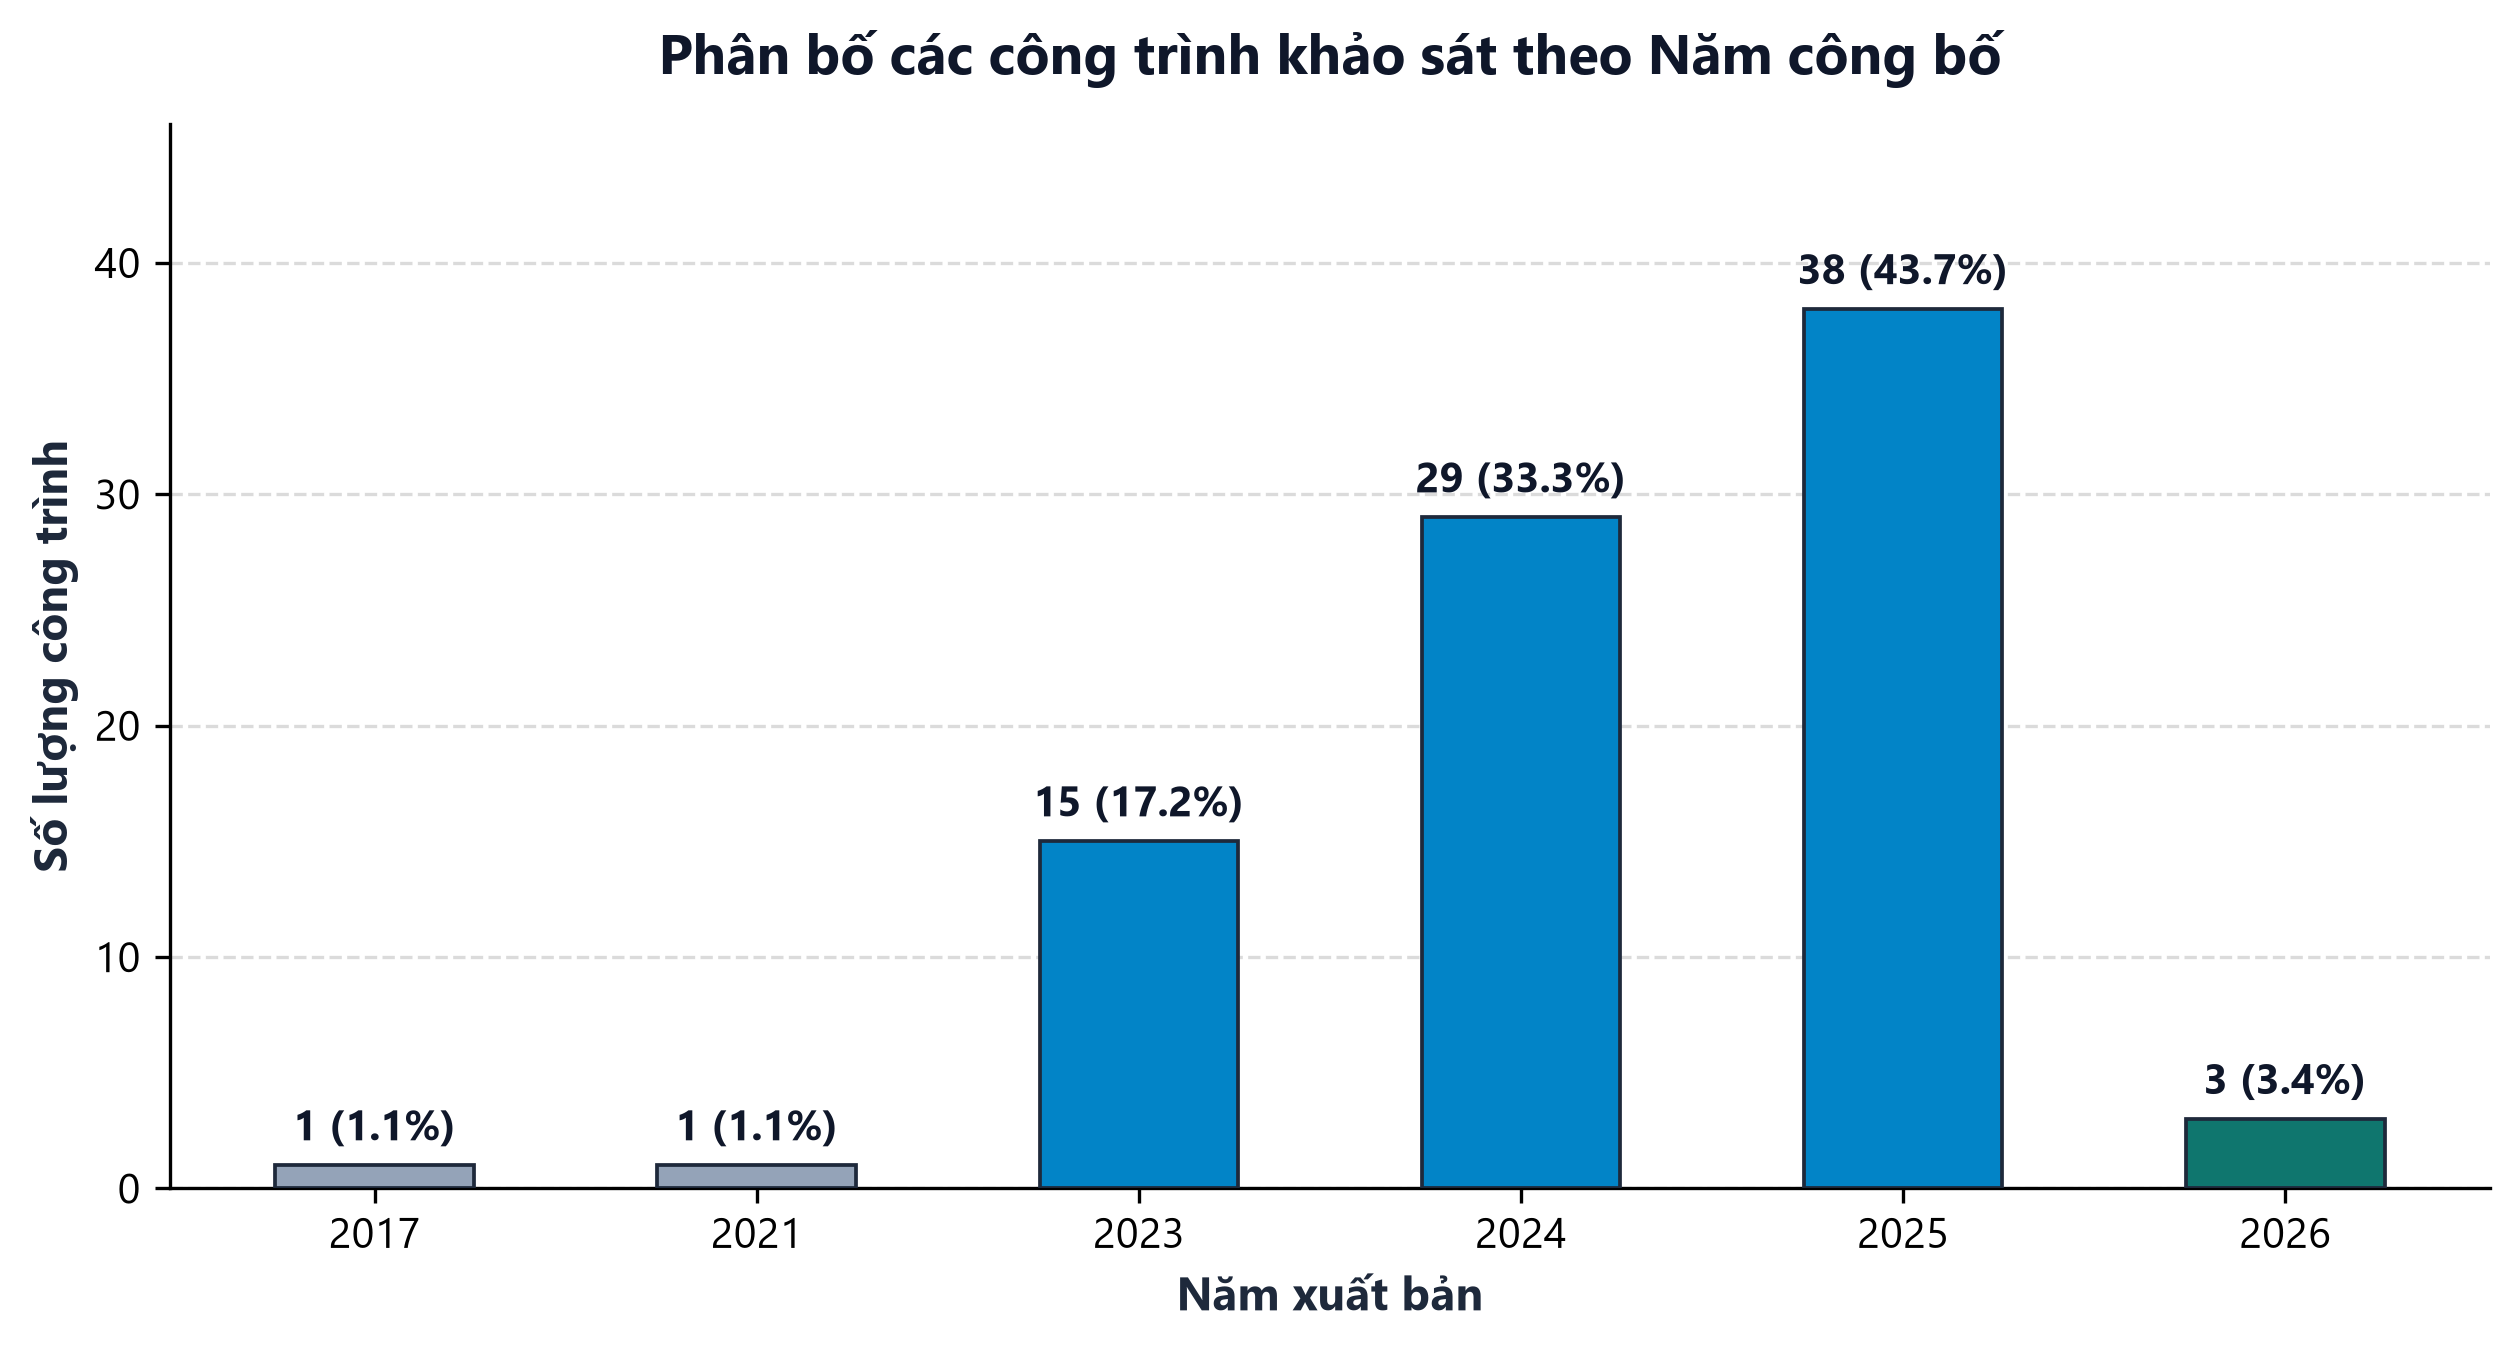
\includegraphics[width=0.86\textwidth]{figures/fig1_distribution_by_year.png}
    \caption{Phân bố các công trình khảo sát thuần Văn bản và Đồ thị theo năm công bố (2017--2026)}
    \label{fig:survey-year}
\end{figure}

\begin{figure}[htbp]
    \centering
    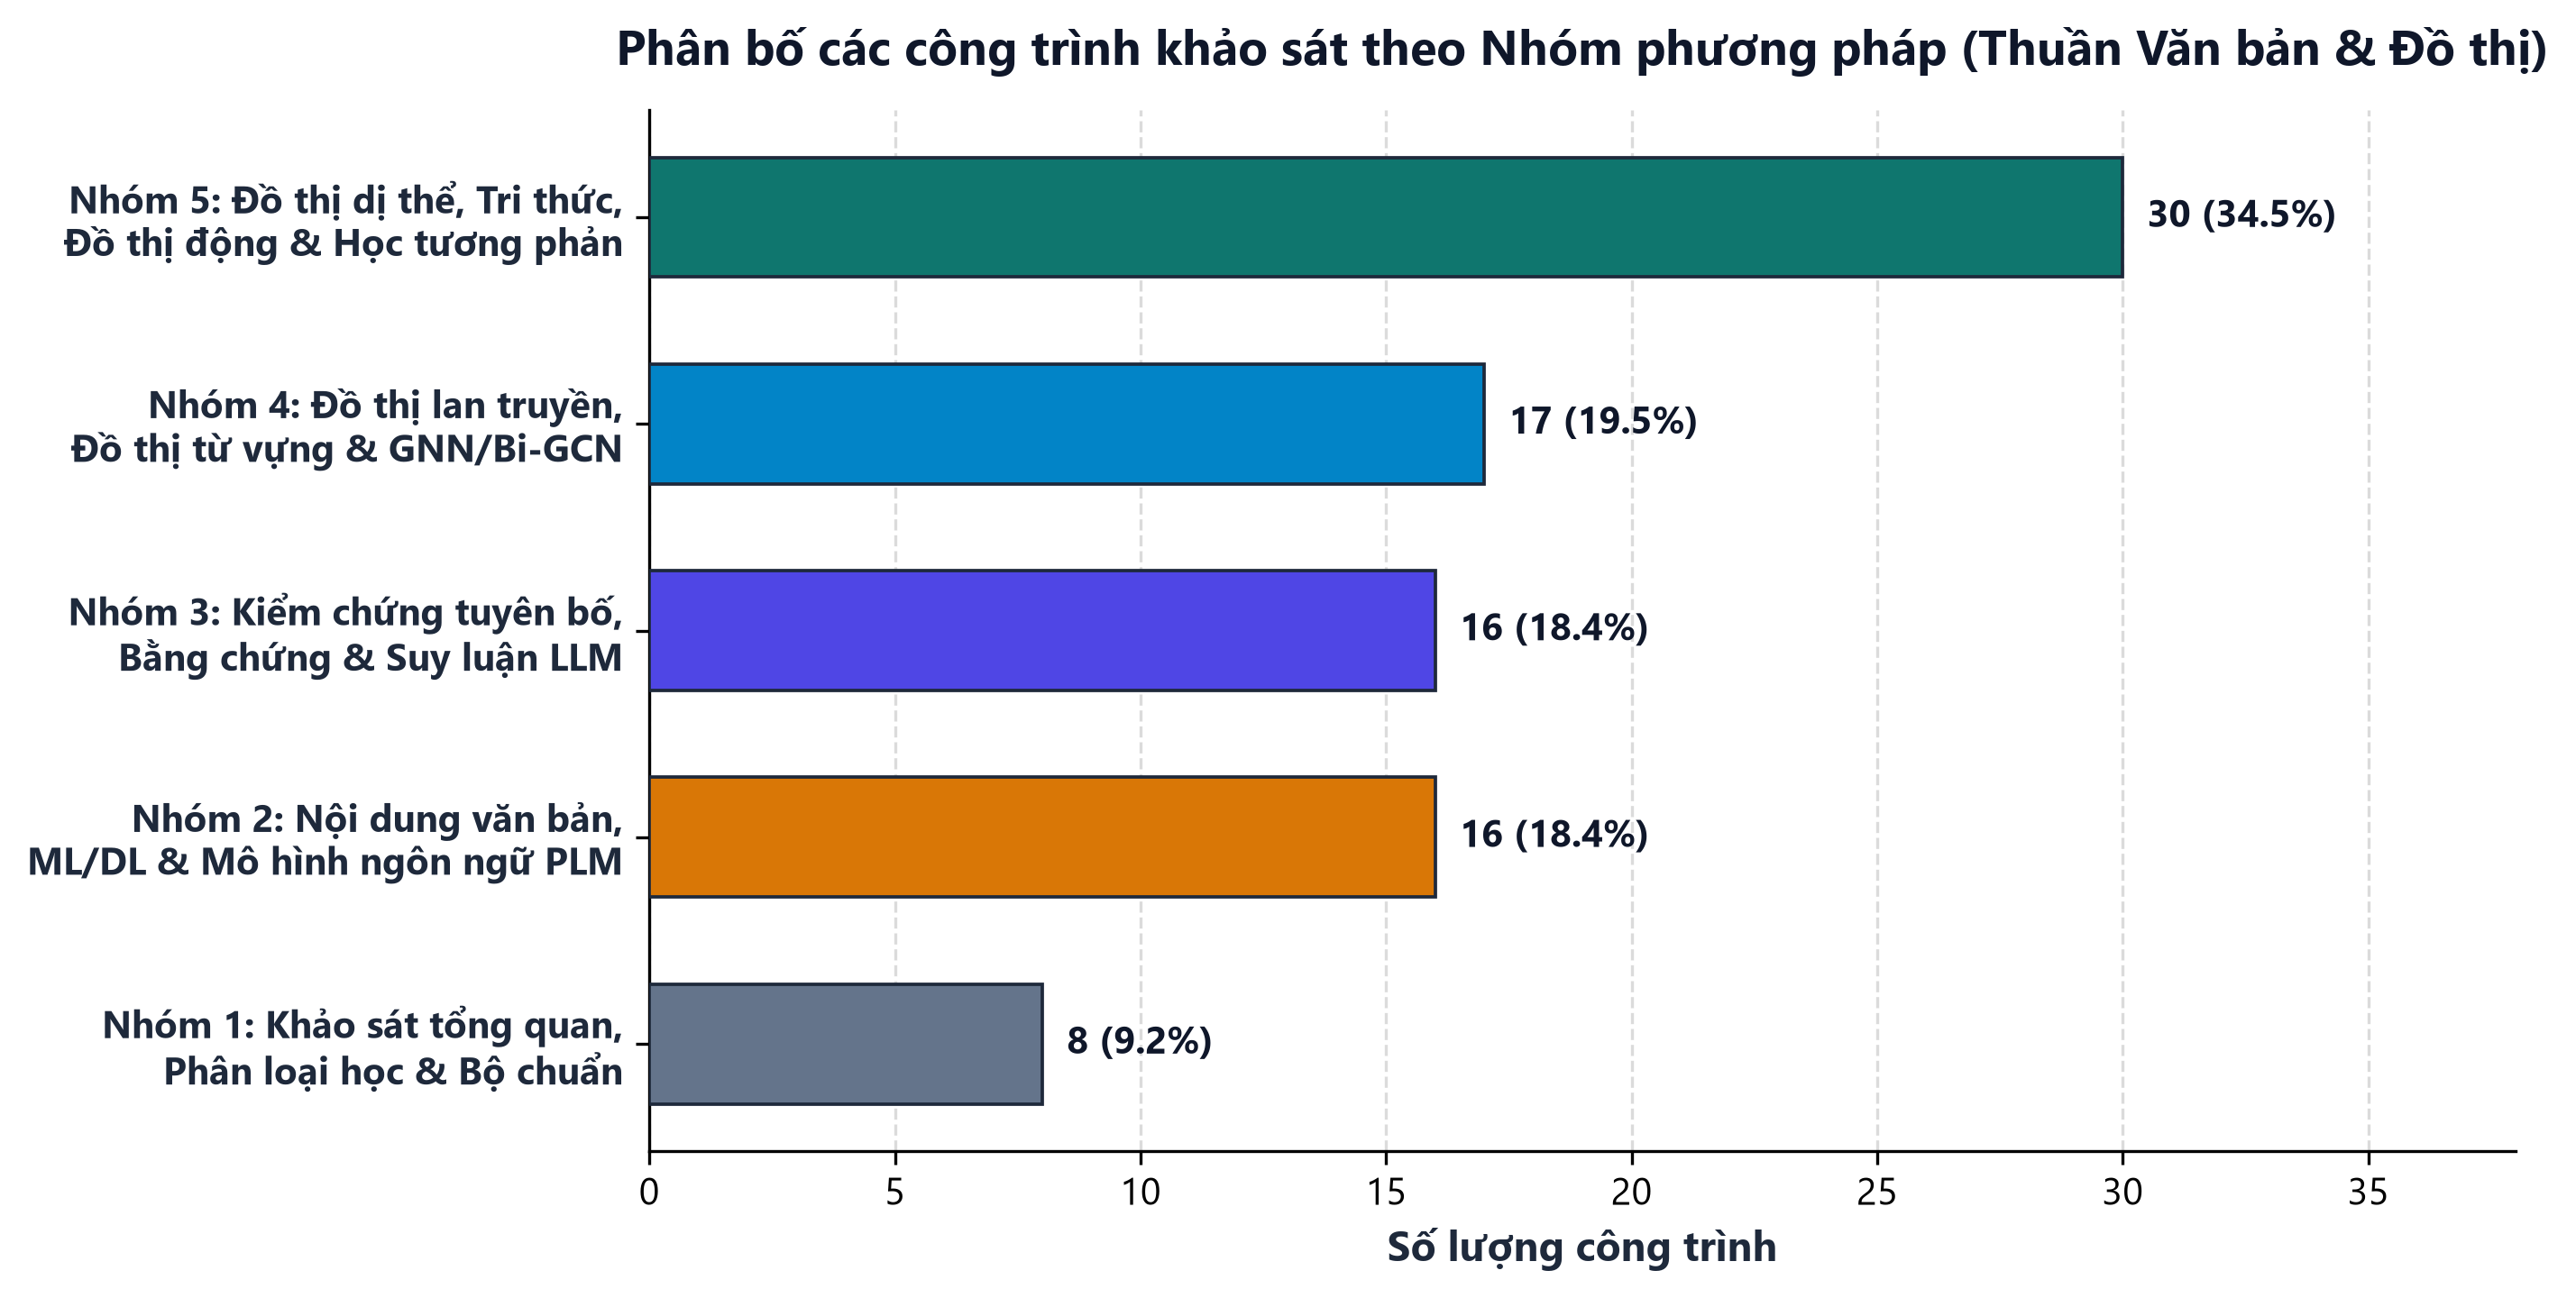
\includegraphics[width=0.88\textwidth]{figures/fig2_distribution_by_method.png}
    \caption{Phân bố các công trình khảo sát theo 05 nhóm phương pháp tiếp cận thuần Văn bản và Đồ thị}
    \label{fig:survey-method}
\end{figure}

\begin{figure}[htbp]
    \centering
    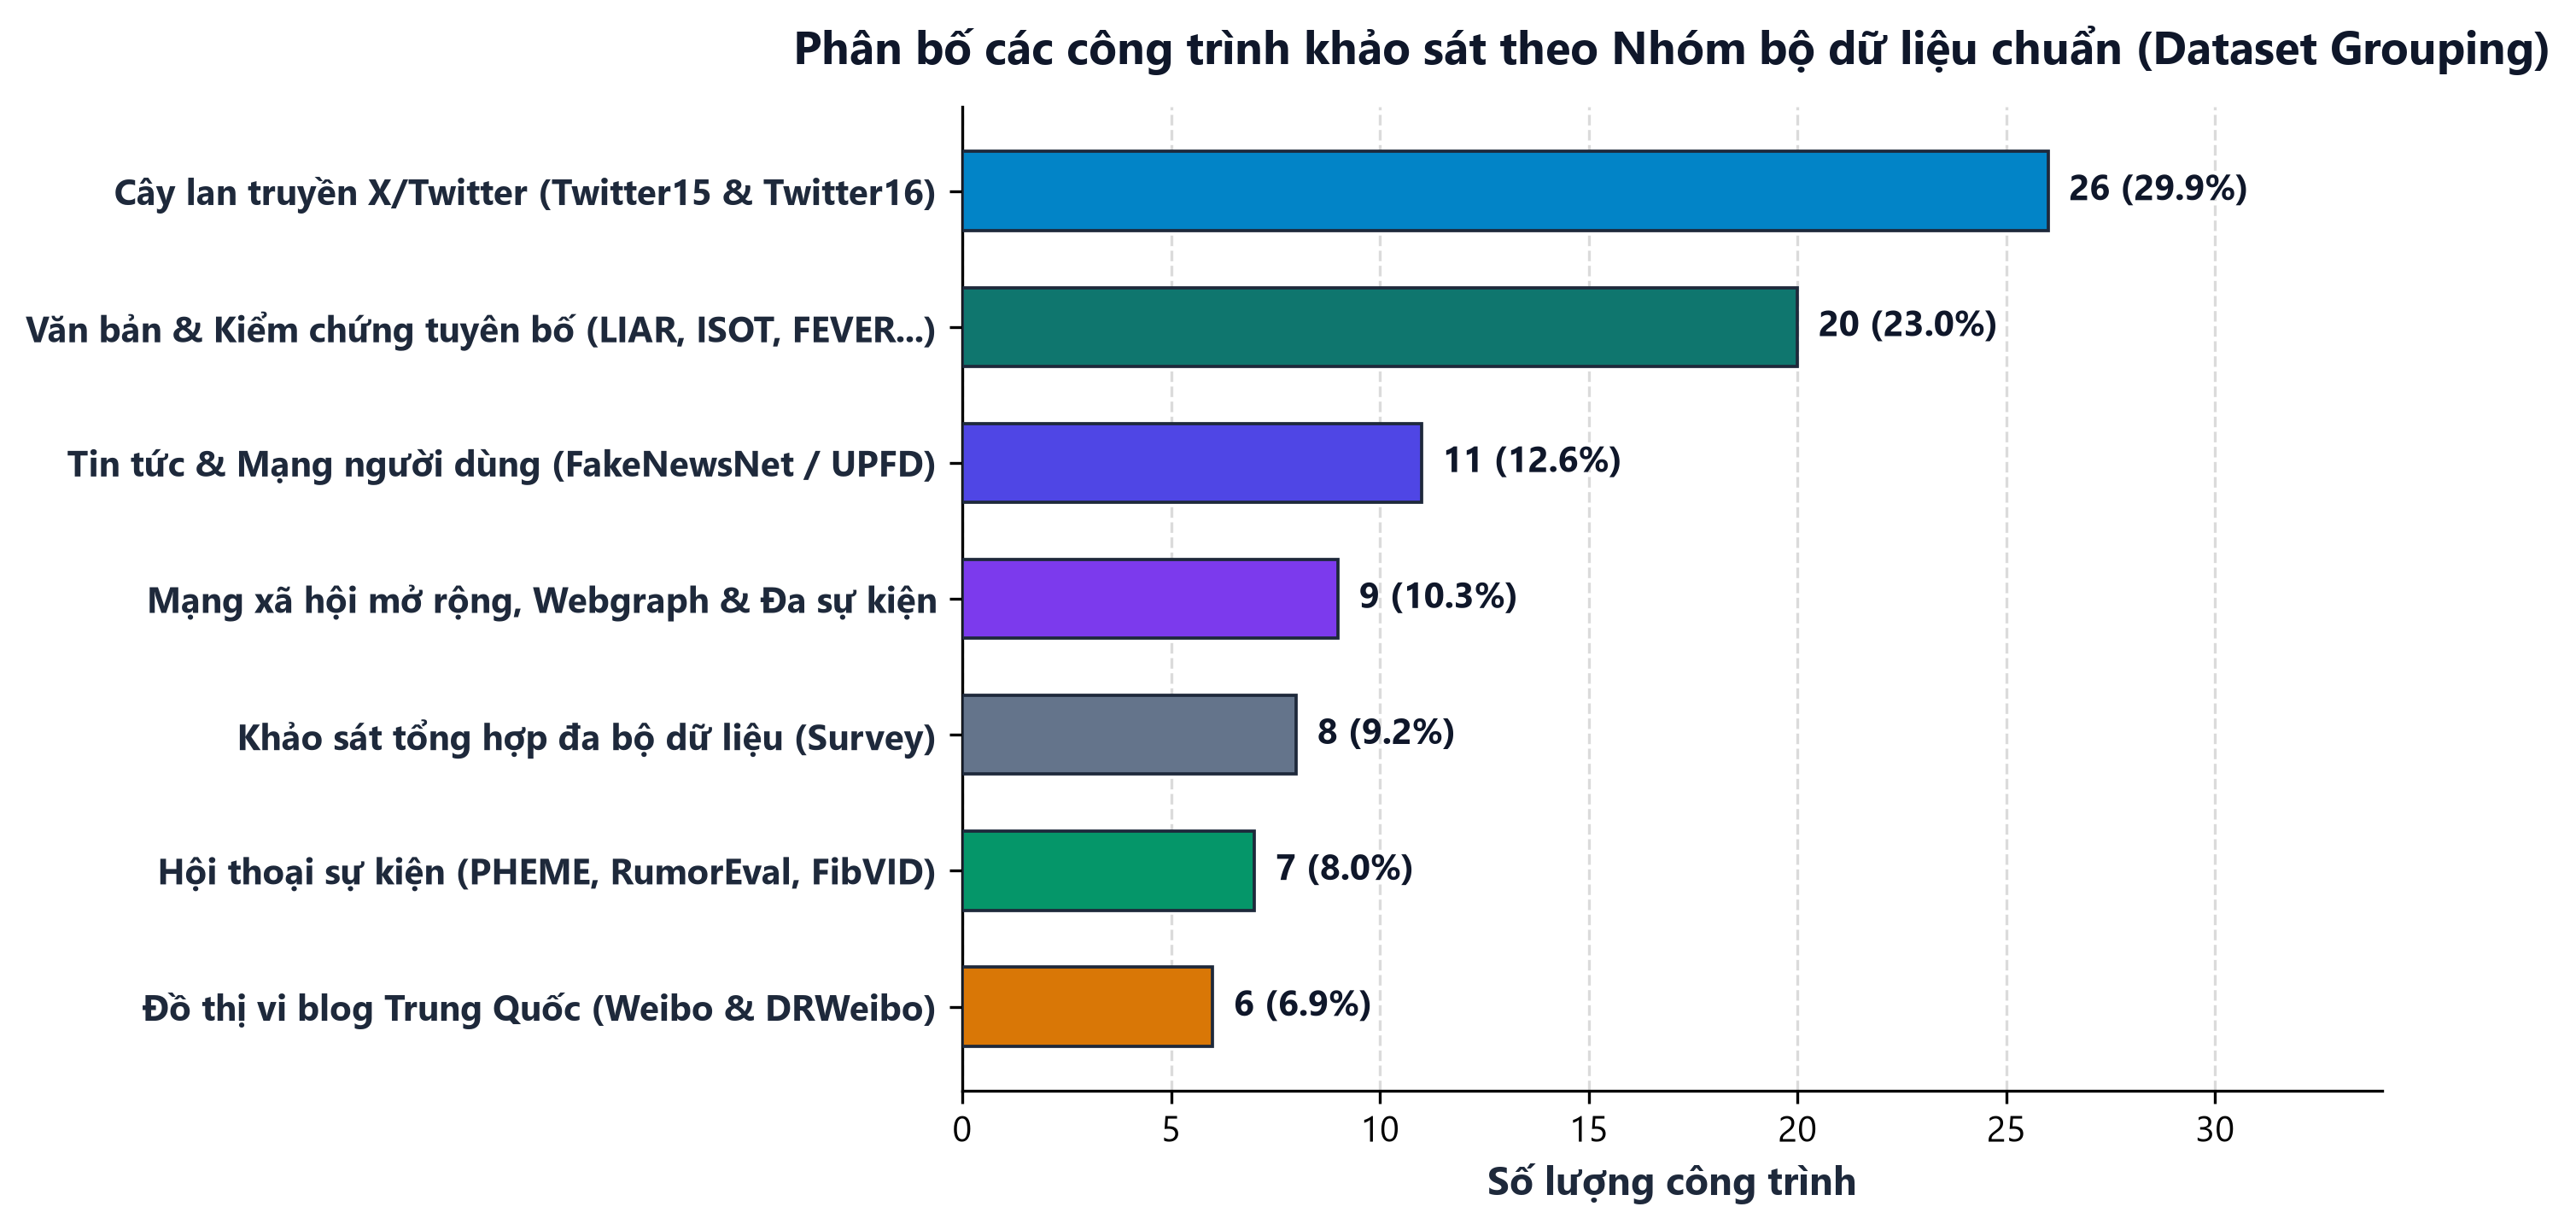
\includegraphics[width=0.88\textwidth]{figures/fig3_distribution_by_dataset.png}
    \caption{Phân bố các công trình khảo sát theo hệ sinh thái bộ dữ liệu chuẩn (Dataset Grouping)}
    \label{fig:survey-dataset}
\end{figure}

\begin{figure}[htbp]
    \centering
    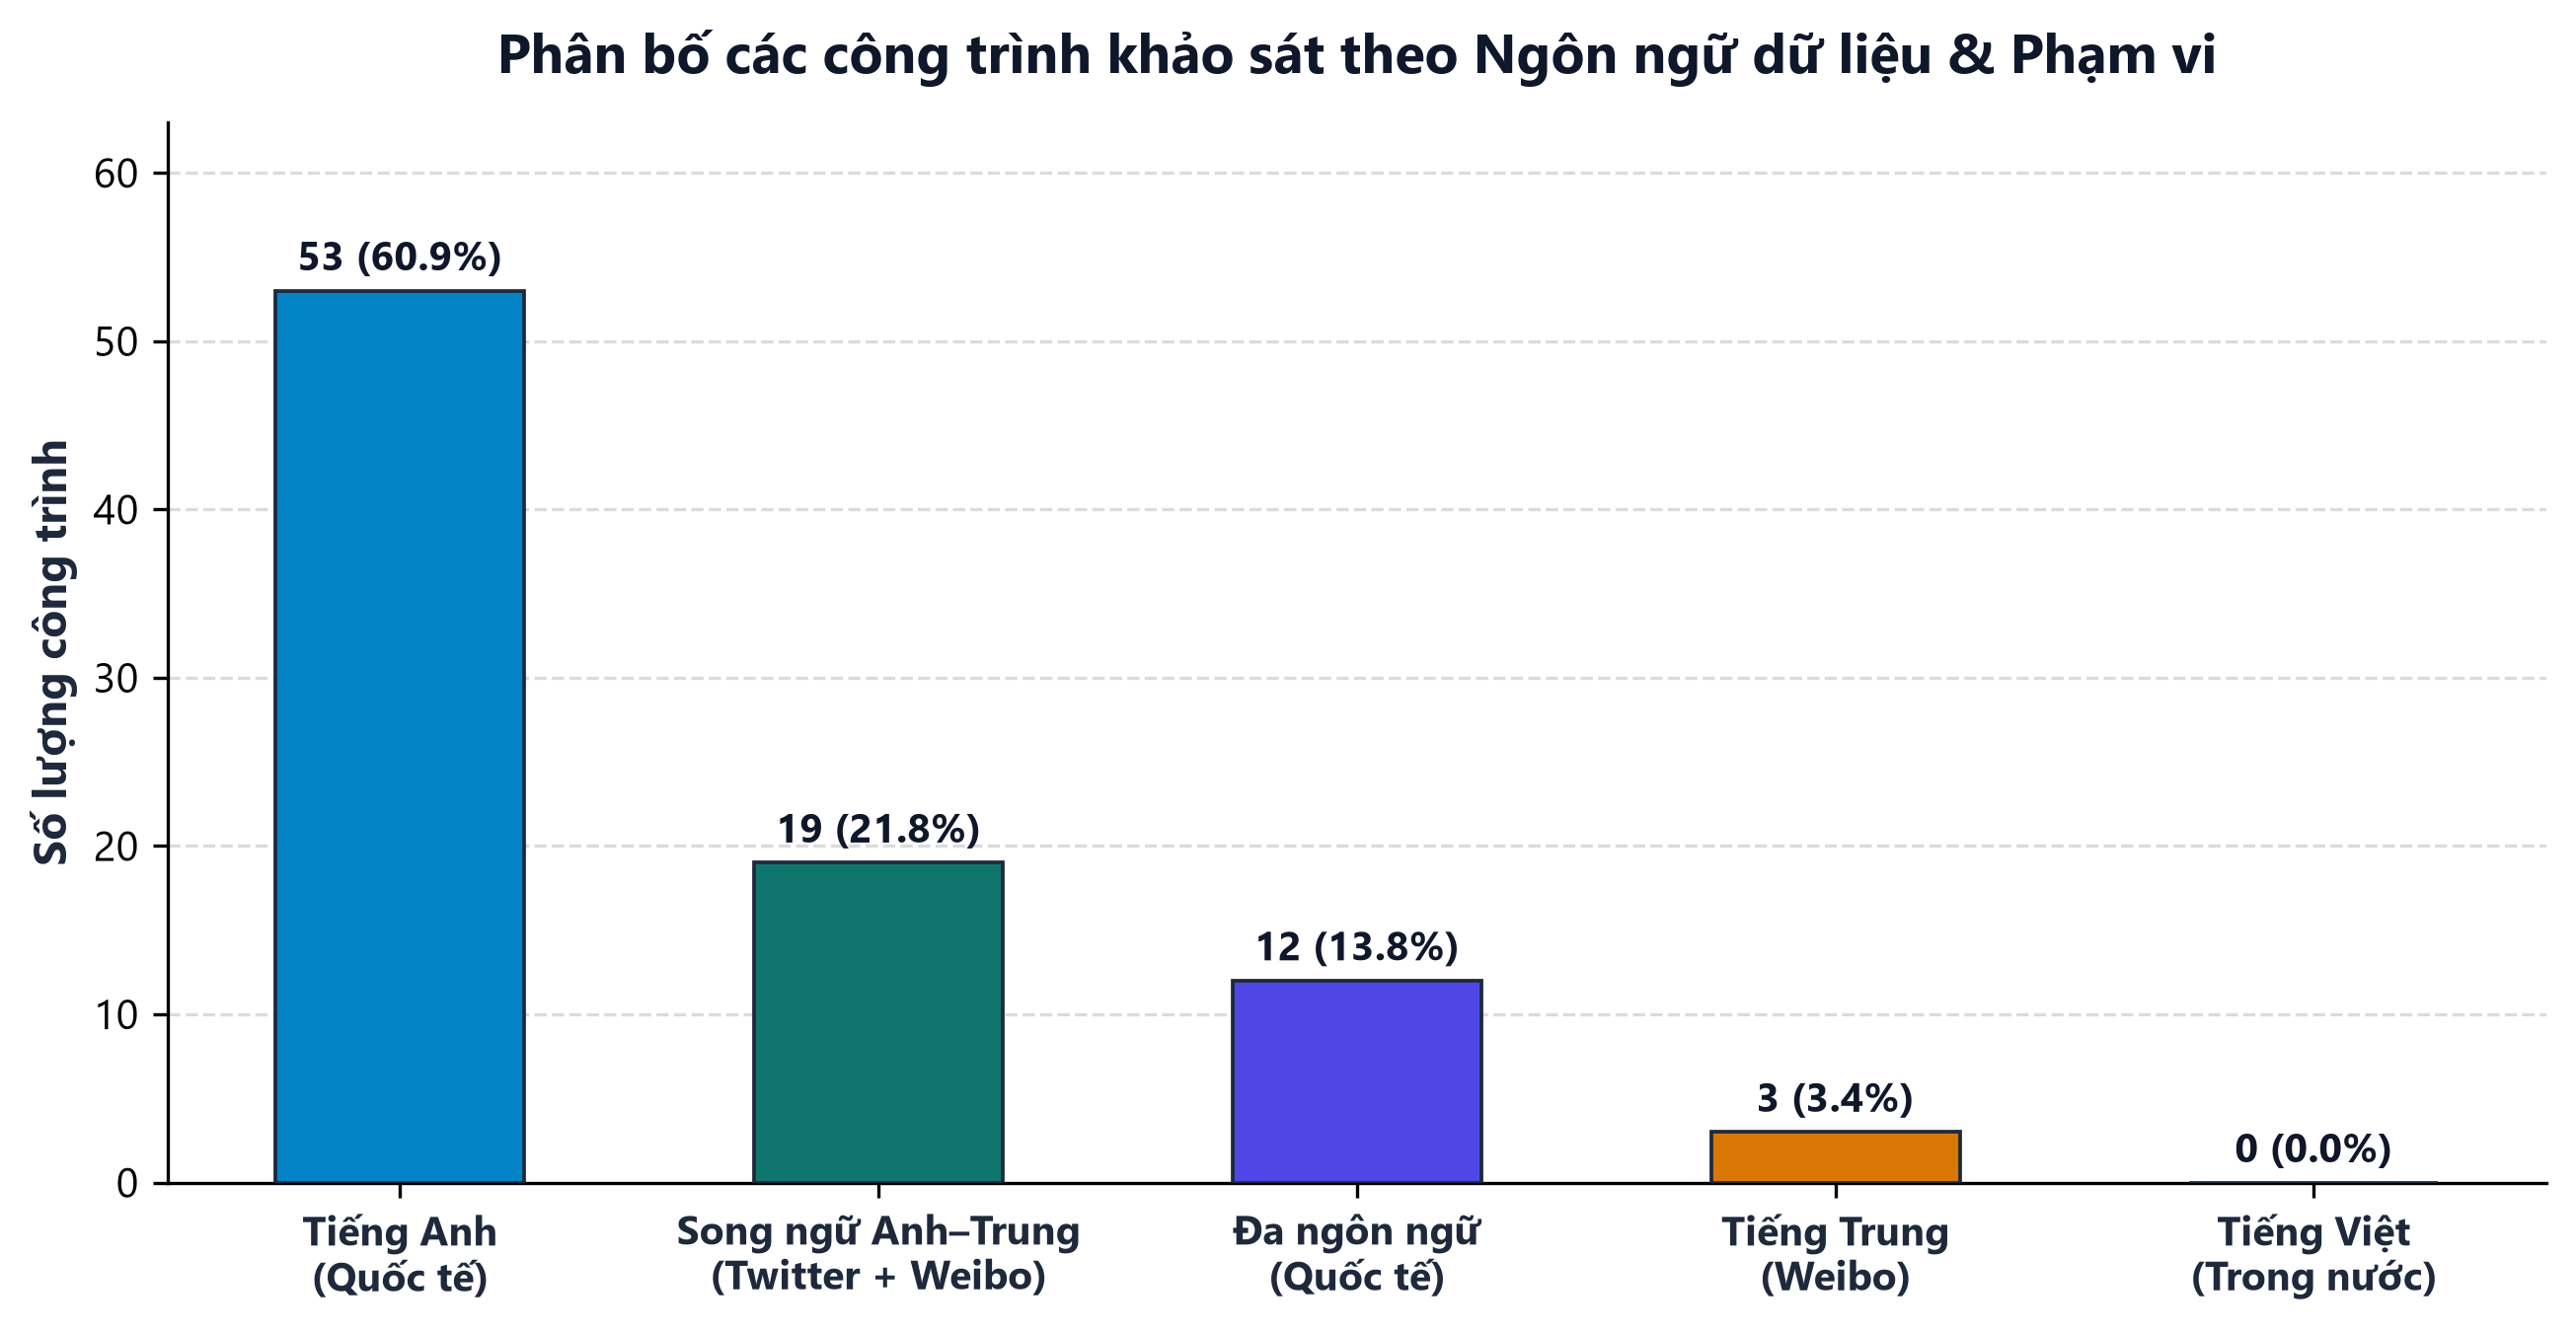
\includegraphics[width=0.86\textwidth]{figures/fig4_distribution_by_language.png}
    \caption{Phân bố các công trình khảo sát theo ngôn ngữ dữ liệu và phạm vi nghiên cứu}
    \label{fig:survey-language}
\end{figure}

\section{Khảo sát, đối chiếu và lựa chọn bộ dữ liệu thực nghiệm}

Để đảm bảo việc lựa chọn dữ liệu thực nghiệm dựa trên căn cứ khoa học chặt chẽ và phù hợp với kiến trúc kết hợp NLP -- Graph Mining, nhóm tiến hành khảo sát, phân tích đặc tính kỹ thuật, ưu/nhược điểm và giao thức đánh giá của các bộ dữ liệu chuẩn phổ biến nhất trong tập các công trình đã tổng hợp, từ đó xác lập bộ dữ liệu chính thức cho đề tài.

\subsection{Tiêu chí đánh giá mức độ phù hợp của bộ dữ liệu}
Dựa trên mục tiêu của đề tài là kết hợp Xử lý ngôn ngữ tự nhiên (NLP) và Phân tích cấu trúc đồ thị lan truyền (Graph Mining), một bộ dữ liệu ứng viên được đánh giá dựa trên năm tiêu chí:
\begin{enumerate}
    \item \textbf{Tính kết hợp song hành Văn bản -- Đồ thị lan truyền:} Bộ dữ liệu phải cung cấp đồng thời cả nội dung văn bản (hoặc đặc trưng nhúng văn bản chuẩn hóa từ bài viết/bình luận) và thông tin liên kết để dựng đồ thị lan truyền (cây retweet/reply hoặc mạng tương tác người dùng -- bài đăng) \cite{noauthor_disinformation_2024, noauthor_comparative_2024}.
    \item \textbf{Quy mô mẫu và tính cân bằng phân lớp:} Số lượng sự kiện/bản tin và số lượng nút/cạnh trên đồ thị phải đủ lớn để huấn luyện mạng học sâu, đồng thời tỷ lệ giữa các lớp (Fake/Real hoặc N/F/T/U) cần tương đối cân bằng để tránh thiên lệch mô hình \cite{noauthor_fake_2024, noauthor_co-attention_2025}.
    \item \textbf{Tính khả dụng và khả năng tái lập hiện tại (Reproducibility):} Do chính sách siết chặt API của X (Twitter) và sự xóa bỏ các tweet/tài khoản vi phạm theo thời gian, các bộ dữ liệu chỉ công bố danh sách Tweet IDs thô thường bị mất mát dữ liệu nghiêm trọng khi thu thập lại \cite{noauthor_exploiting_2024}. Do đó, cần ưu tiên các bộ dữ liệu đã được đóng gói sẵn cấu trúc đồ thị và đặc trưng nút (như trong thư viện \texttt{PyTorch-Geometric}) hoặc các kho lưu trữ giữ nguyên tệp JSON cây hội thoại \cite{noauthor_ensemble_2024, noauthor_co-attention_2025}.
    \item \textbf{Mức độ chuẩn hóa trong cộng đồng nghiên cứu:} Được sử dụng rộng rãi trong các bài báo Q1/Hội nghị hàng đầu 5 năm gần đây, giúp nhóm có sẵn các con số baseline chuẩn (như Bi-GCN, GAT, GraphSAGE, UPFD, BERT) để đối chiếu kết quả \cite{noauthor_fake_2024, noauthor_co-attention_2025}.
    \item \textbf{Sự rõ ràng về cách chia dữ liệu và độ đo đánh giá:} Có giao thức chia tập Train/Validation/Test hoặc K-Fold Cross-Validation tường minh cùng hệ thống độ đo chuẩn (Accuracy, Precision, Recall, F1-score, AUC-ROC) \cite{noauthor_comparative_2024, noauthor_integrating_2025}.
\end{enumerate}

\subsection{Phân tích chi tiết các bộ dữ liệu ứng viên}

\subsubsection{1. Bộ dữ liệu FakeNewsNet (PolitiFact \& GossipCop) và bản đóng gói đồ thị UPFD}
\begin{itemize}
    \item \textbf{Nguồn gốc và quy mô gốc:} FakeNewsNet do Shu và cộng sự giới thiệu là kho dữ liệu đa chiều thu thập từ hai tổ chức kiểm chứng sự thật uy tín là PolitiFact (lĩnh vực chính trị Mỹ) và GossipCop (lĩnh vực tin tức giải trí/người nổi tiếng), với tổng quy mô báo cáo trong khảo sát của Lakzaei và cộng sự (2024) là 23,901 bản tin thuộc 2 nhãn nhị phân \texttt{\{fake, real\}} \cite{noauthor_disinformation_2024, noauthor_improving_2025}. Trong khảo sát của Moorthy và cộng sự (2025) \cite{noauthor_dual_2025}, tập con PolitiFact bao gồm 900 bài báo chính trị với 95,553 người dùng đăng tweet, 113,473 lượt thích (likes), 106,195 lượt chia sẻ lại (retweets) và 40,585 lượt trả lời (replies); tập con GossipCop gồm 420 bài có văn bản, 336 bài có ảnh, 164,892 tweets, 11,975 replies và 31,692 likes.
    \item \textbf{Phiên bản đồ thị UPFD (User Preference-aware Fake News Detection):} Do FakeNewsNet gốc hiện bị mất mát dữ liệu khi cào lại qua Twitter API \cite{noauthor_exploiting_2024}, Dou và cộng sự (được sử dụng trực tiếp trong \cite{noauthor_ensemble_2024, noauthor_co-attention_2025}) đã biên soạn và đóng gói bộ dữ liệu đồ thị UPFD tích hợp sẵn trong thư viện \texttt{PyTorch-Geometric}. Theo số liệu thống kê trong Bảng 1 của nghiên cứu CMCG (2025) \cite{noauthor_co-attention_2025}:
    \begin{itemize}
        \item \textit{Nhánh PolitiFact (UPFD):} Gồm 314 đồ thị bản tin được cân bằng tuyệt đối (157 tin giả và 157 tin thật), tổng cộng 41,054 nút và 40,740 cạnh.
        \item \textit{Nhánh GossipCop (UPFD):} Gồm 5,464 đồ thị bản tin được cân bằng tuyệt đối (2,732 tin giả và 2,732 tin thật), tổng cộng 314,262 nút và 308,798 cạnh.
        \item \textit{Đặc trưng nút đi kèm:} Mỗi bản tin là một đồ thị cây lan truyền có nút gốc là bài đăng bản tin và các nút con là người dùng chia sẻ nó. Bộ dữ liệu cung cấp sẵn 4 loại đặc trưng nút: (1) 768 đặc trưng BERT mã hóa từ bài tin và 200 tweets lịch sử của người dùng; (2) 300 đặc trưng Word2Vec/SpaCy; (3) 10 đặc trưng thuộc tính hồ sơ người dùng (thời gian tạo tài khoản, vị trí địa lý, số người theo dõi, số người đang theo dõi, trạng thái xác minh, điểm Botometer, tỷ lệ follower/followee, số tweet đã đăng, số lượt thích); và (4) đặc trưng kết hợp \texttt{spaCy+Profile} (310 chiều) \cite{noauthor_ensemble_2024, noauthor_co-attention_2025}.
    \end{itemize}
    \item \textbf{Cách chia dữ liệu và Độ đo:} Các nghiên cứu trên UPFD và FakeNewsNet thường chia theo tỷ lệ chuẩn (Train/Val/Test tích hợp sẵn trong PyG hoặc 80\% Train -- 20\% Test) hoặc Stratified K-Fold Cross-Validation, sử dụng các độ đo nhị phân: Accuracy (ACC), Precision, Recall, F1-score, AUC-ROC và hệ số tương quan Matthews (MCC) \cite{noauthor_ensemble_2024, noauthor_comparative_2024, noauthor_co-attention_2025}.
\end{itemize}

\subsubsection{2. Bộ dữ liệu Twitter15 và Twitter16}
\begin{itemize}
    \item \textbf{Nguồn gốc và quy mô:} Do Ma và cộng sự (2017) \cite{ma_detect_2017} xây dựng từ nền tảng Twitter, bao gồm 1,490 sự kiện/cây hội thoại trong Twitter15 và 818 sự kiện/cây hội thoại trong Twitter16 \cite{noauthor_disinformation_2024, ma_detect_2017}.
    \item \textbf{Số lượng phân lớp và đặc điểm:} Khác với bài toán nhị phân, Twitter15 và Twitter16 được gán nhãn chi tiết vào 4 phân lớp cân bằng: Tin đồn đúng (\textit{True rumor -- TR}), Tin đồn sai (\textit{False rumor -- FR}), Tin đồn chưa kiểm chứng (\textit{Unverified rumor -- UR}) và Không phải tin đồn (\textit{Non-rumor -- NR}) (một số nghiên cứu như ICP-BGCN 2025 \cite{noauthor_integrating_2025} cũng thực hiện gộp TR, FR, UR thành nhóm Rumors để so sánh nhị phân với NR). Mỗi mẫu cung cấp văn bản của bài tweet gốc và cấu trúc cây lan truyền có hướng (ai retweet hoặc reply ai kèm mốc thời gian) \cite{noauthor_early_2025, noauthor_integrating_2025}.
    \item \textbf{Cách chia dữ liệu và Độ đo:} Giao thức chuẩn trên Twitter15/16 là chia 5-fold cross-validation; đánh giá bằng Accuracy tổng thể, Macro-F1 và điểm F1 riêng cho từng lớp trong 4 lớp $\{N, F, T, U\}$ \cite{noauthor_early_2025, noauthor_integrating_2025, noauthor_beyond_2023}.
\end{itemize}

\subsubsection{3. Bộ dữ liệu PHEME và Sina Weibo}
\begin{itemize}
    \item \textbf{PHEME:} Gồm các chuỗi hội thoại (conversation threads) trên Twitter thu thập theo các sự kiện tin tức nóng (breaking news events) thuộc lĩnh vực chính trị và xã hội, được gán nhãn ở mức 2 lớp (Rumor / Non-rumor) hoặc 4 lớp chi tiết \cite{noauthor_fake_2023, noauthor_disinformation_2024, noauthor_detection_2025}. Ưu điểm lớn của PHEME là lưu trữ nguyên vẹn các tệp JSON văn bản của tweet nguồn và toàn bộ bình luận phản hồi trực tiếp, cho phép chạy trực tiếp các mô hình BERT/RoBERTa trên từng nút bình luận mà không cần gọi lại Twitter API.
    \item \textbf{Sina Weibo:} Do Ma và cộng sự (2016) thu thập từ mạng xã hội Weibo (Trung Quốc), gồm 4,664 sự kiện chia làm 2 lớp nhị phân \texttt{\{fake, real\}}, bao gồm văn bản bài đăng tiếng Trung và đồ thị cây lan truyền quy mô lớn \cite{noauthor_disinformation_2024, noauthor_detection_2025}. Các mô hình như Bi-GCN đạt Accuracy tới 0.961 trên bộ dữ liệu này \cite{noauthor_detection_2025}. Tuy nhiên, do ngôn ngữ là tiếng Trung nên bộ dữ liệu này chủ yếu phục vụ khi muốn kiểm chứng khả năng đa ngôn ngữ của mô hình \cite{noauthor_semantic_2025-1, lin_unified_2023}.
\end{itemize}

\subsubsection{4. Bộ dữ liệu FibVID và tập sự kiện đồ thị mở rộng}
\begin{itemize}
    \item \textbf{FibVID:} Bộ dữ liệu đánh giá các phương pháp dựa trên lan truyền xoay quanh chủ đề COVID-19 và chính trị (kiểm chứng bởi PolitiFact và Snopes) \cite{noauthor_exploiting_2024}. Trong nghiên cứu của Soga và cộng sự (2024) \cite{noauthor_exploiting_2024}, sau khi lọc bỏ các tweet có độ tương đồng Word2Vec $<0.3$ và cân bằng lớp, tập dữ liệu gồm 553 đồ thị (276 Real, 277 Fake) với số nút trung bình là 172 nút/đồ thị, số cạnh trung bình là 513 cạnh/đồ thị, độ sâu tối đa trung bình 1.834 (lớn nhất bằng 6) và bậc nút trung bình 5.823.
    \item \textbf{DRWeibo và Weibo-COVID19 / Twitter-COVID19:} Các biến thể mở rộng của đồ thị lan truyền mạng xã hội không nhãn hoặc theo sự kiện dịch chuyển miền (OOD), được sử dụng phổ biến trong các nghiên cứu học tương phản và thích nghi thời điểm kiểm thử (\textit{Test-Time Adaptation}) giai đoạn 2024--2026 \cite{cui_avoiding_2026, cui_graph_2025, tao_out--distribution_2024}.
\end{itemize}

\subsubsection{5. Nhóm bộ dữ liệu thuần văn bản quy mô lớn (ISOT, LIAR, ConFake)}
\begin{itemize}
    \item \textbf{ISOT Dataset:} Do phòng thí nghiệm ISOT (Đại học Victoria) biên soạn, gồm khoảng 44,898 -- 45,000 bài báo tiếng Anh (giai đoạn 2016--2017), chia cân bằng giữa tin thật (từ Reuters) và tin giả (từ các trang bị PolitiFact và Wikipedia gắn cờ) \cite{noauthor_comparative_2024, noauthor_hybrid_2025}. Mỗi mẫu có tiêu đề, toàn văn, ngày đăng và chủ đề nhưng \textbf{không có sẵn thông tin đồ thị lan truyền mạng xã hội} \cite{noauthor_comparative_2024}.
    \item \textbf{LIAR Dataset:} Do Wang (2017) công bố, gồm 12,836 tuyên bố chính trị ngắn từ PolitiFact kèm thông tin người phát ngôn (tên, nghề nghiệp, đảng phái, bang, lịch sử tín nhiệm), được gán nhãn cân bằng vào 6 lớp mức độ chân thực (\textit{true, mostly-true, half-true, barely-true, false, pants-fire}) \cite{noauthor_fake_2023, noauthor_comprehensive_2024}. Tương tự ISOT, LIAR không có cây lan truyền tương tác người dùng.
    \item \textbf{ConFake Dataset:} Do Jain và cộng sự (2023) tổng hợp từ 5 nguồn (Kaggle, Reuters, McIntire, BuzzFeed, PolitiFact) với tổng cộng 72,455 bài báo (35,185 bài thật và 37,270 bài giả) nhằm giảm hiện tượng quá khớp (overfitting) cho các mô hình phân loại văn bản \cite{noauthor_hybrid_2025}.
\end{itemize}

\subsection{Bảng tổng hợp và đối chiếu các bộ dữ liệu chuẩn}
Bảng \ref{tab:dataset-candidates} tổng hợp các thông số kỹ thuật, quy mô mẫu, cấu trúc văn bản -- đồ thị, giao thức chia dữ liệu, độ đo đánh giá và nhận định phân tích đối với các bộ dữ liệu chuẩn trong lĩnh vực.

\begin{landscape}
\footnotesize
\renewcommand{\arraystretch}{1.35}
\setlength{\tabcolsep}{4pt}
\begin{longtable}{@{}p{2.8cm}p{2.2cm}p{2.8cm}p{3.8cm}p{3.2cm}p{3.6cm}p{4.2cm}@{}}
\caption{Bảng tổng hợp và đối chiếu đặc tính kỹ thuật của các bộ dữ liệu chuẩn trong bài toán phát hiện tin giả và tin đồn trên mạng xã hội}
\label{tab:dataset-candidates}\\
\toprule
\textbf{Tên Dataset} & \textbf{Lĩnh vực \& Nền tảng} & \textbf{Quy mô mẫu \& Số phân lớp} & \textbf{Đặc điểm dữ liệu (Văn bản \& Đồ thị)} & \textbf{Cách chia dữ liệu \& Độ đo chuẩn} & \textbf{Các công bố tiêu biểu đã có kết quả} & \textbf{Nhận định phân tích (Ưu / Nhược điểm khi chọn)} \\
\toprule
\endfirsthead
\multicolumn{7}{l}{\textbf{Bảng \ref{tab:dataset-candidates} (tiếp theo)}}\\
\toprule
\textbf{Tên Dataset} & \textbf{Lĩnh vực \& Nền tảng} & \textbf{Quy mô mẫu \& Số phân lớp} & \textbf{Đặc điểm dữ liệu (Văn bản \& Đồ thị)} & \textbf{Cách chia dữ liệu \& Độ đo chuẩn} & \textbf{Các công bố tiêu biểu đã có kết quả} & \textbf{Nhận định phân tích (Ưu / Nhược điểm khi chọn)} \\
\toprule
\endhead
\toprule
\bottomrule \endlastfoot

\textbf{UPFD (PolitiFact \& GossipCop trong PyG)} \cite{noauthor_ensemble_2024, noauthor_co-attention_2025} & Chính trị, Giải trí / Twitter & \textbf{PolitiFact:} 314 đồ thị (157 Fake / 157 Real; 41,054 nút; 40,740 cạnh).\newline \textbf{GossipCop:} 5,464 đồ thị (2,732 Fake / 2,732 Real; 314,262 nút; 308,798 cạnh).\newline \textbf{Phân lớp:} 2 lớp (Nhị phân). & Mỗi bản tin là một đồ thị cây lan truyền người dùng chia sẻ. Đã trích xuất sẵn đặc trưng nút: BERT (768d), SpaCy (300d), User Profile (10d) và SpaCy+Profile (310d). & Chia Train / Val / Test cố định trong PyTorch-Geometric hoặc 80/20.\newline \textbf{Độ đo:} ACC, Precision, Recall, F1-score, AUC, MCC. & Dou et al. (2021) -- UPFD; Malik et al. (2024) -- EGNN \cite{noauthor_ensemble_2024}; CMCG (2025) (ACC 96.77\% PolitiFact, 98.53\% GossipCop) \cite{noauthor_co-attention_2025}. & \textbf{Ưu:} Tải trực tiếp bằng code thông qua \texttt{torch\_\allowbreak geometric.\allowbreak datasets.\allowbreak UPFD}, không bị lỗi mất tweet do khóa API, cân bằng lớp tuyệt đối.\newline \textbf{Nhược:} Đặc trưng văn bản đã được nén sẵn thành vector nên không can thiệp lại bước tiền xử lý câu chữ thô ban đầu. \\ 

\textbf{FakeNewsNet (Bản gốc / Chuyển đổi KG)} \cite{noauthor_disinformation_2024, noauthor_dual_2025, noauthor_improving_2025} & Chính trị, Giải trí / PolitiFact, GossipCop, Twitter & Tổng 23,901 bản tin (trong \cite{noauthor_dual_2025} dùng 900 bài PolitiFact với 164,892 tweets GossipCop).\newline \textbf{Phân lớp:} 2 lớp (\texttt{fake, real}). & Gồm toàn văn bài báo, tiêu đề, nguồn tin và mạng tương tác người dùng (likes, retweets, replies). Có thể chuyển thành đồ thị dị thể hoặc KG (qua RML). & Stratified K-Fold CV hoặc chia Train/Test.\newline \textbf{Độ đo:} ACC, Precision, Recall, F1-score, AUC-ROC. & Shu et al. (2020); Golovin et al. (2025) -- GAT+KG (F1 95\%) \cite{noauthor_improving_2025}; Moorthy et al. (2025) -- BERT-GNN (ACC 99\%) \cite{noauthor_dual_2025}. & \textbf{Ưu:} Cho phép tự xây dựng đồ thị dị thể đa thực thể (Article-User-Source-Hashtag) và chạy BERT trực tiếp từ văn bản thô.\newline \textbf{Nhược:} Dữ liệu tweet thu thập lại qua API bị hao hụt nhiều \cite{noauthor_exploiting_2024}, cần dùng các bản snapshot đã lưu trữ sẵn trên GitHub/Kaggle. \\ 

\textbf{Twitter15 \& Twitter16} \cite{noauthor_disinformation_2024, noauthor_early_2025, noauthor_integrating_2025, ma_detect_2017} & Xã hội đa chủ đề / Twitter & \textbf{Twitter15:} 1,490 sự kiện.\newline \textbf{Twitter16:} 818 sự kiện.\newline \textbf{Phân lớp:} 4 lớp (\textit{True, False, Unverified, Non-rumor}) hoặc gộp 2 lớp. & Cung cấp văn bản tweet gốc, danh sách phản hồi và cấu trúc cây lan truyền có hướng kèm dấu thời gian (top-down \& bottom-up propagation trees). & 5-fold Cross-Validation.\newline \textbf{Độ đo:} Accuracy, Macro-F1 và F1 riêng cho từng lớp (TR, FR, UR, NR). & Ma et al. (2017) -- PTK \cite{ma_detect_2017}; EBGCN \cite{wei_towards_2021}; RAGCL \cite{cui_propagation_2024}; Early-GCN \cite{noauthor_early_2025}; ICP-BGCN \cite{noauthor_integrating_2025}; TRGCN \cite{yan_trgcn_2026}. & \textbf{Ưu:} Là bộ benchmark kinh điển nhất cho bài toán phân tích cấu trúc cây lan truyền hai chiều (Bi-GCN) và hỗ trợ mốc thời gian phát tán.\newline \textbf{Nhược:} Quy mô số lượng sự kiện gốc ở mức vừa phải (tổng cộng 2,308 sự kiện). \\ 

\textbf{PHEME} \cite{noauthor_fake_2023, noauthor_detection_2025} & Chính trị, Sự kiện xã hội / Twitter & Khoảng 5,802 -- 6,425 chuỗi hội thoại thuộc các sự kiện thời sự lớn.\newline \textbf{Phân lớp:} 2 lớp (Rumor/Non-rumor) hoặc 4 lớp. & Lưu trữ đầy đủ văn bản gốc của tweet nguồn, toàn bộ văn bản các bình luận phản hồi tạo thành cây hội thoại và thông tin người dùng dưới dạng JSON. & 5-fold CV hoặc Leave-one-event-out CV.\newline \textbf{Độ đo:} Accuracy, Precision, Recall, Macro-F1. & Zubiaga et al. (2016); VROC (F1 0.876) \cite{noauthor_detection_2025}; Temporal Tree Transformer \cite{wu_rumor_2025}. & \textbf{Ưu:} Có sẵn toàn bộ văn bản thô của cả bài gốc lẫn các nút bình luận con, rất thuận lợi để thử nghiệm phân tích lập trường (stance) + GNN.\newline \textbf{Nhược:} Phân bố mẫu giữa các sự kiện không đồng đều, kiểm thử chéo theo sự kiện (cross-event) rất thách thức. \\ 

\textbf{Sina Weibo} \cite{noauthor_disinformation_2024, noauthor_detection_2025} & Xã hội / Weibo (Trung Quốc) & 4,664 sự kiện.\newline \textbf{Phân lớp:} 2 lớp nhị phân (\texttt{fake, real}). & Gồm văn bản bài đăng tiếng Trung và đồ thị cây lan truyền tương tác quy mô lớn trên nền tảng vi blog. & 5-fold Cross-Validation.\newline \textbf{Độ đo:} Accuracy, Precision, Recall, F1-score. & Wu et al. (2015); Ma et al. (2016); Bi-GCN (ACC 0.961) \cite{noauthor_detection_2025}; P2T3 \cite{cui_avoiding_2026}; RAGAT-Mind \cite{qin_ragat-mind_2025}. & \textbf{Ưu:} Cây lan truyền sâu và quy mô tương tác lớn trên từng sự kiện.\newline \textbf{Nhược:} Văn bản bằng tiếng Trung nên phải dùng mô hình tiếng Trung (như \texttt{bert-base-chinese}), không trực quan khi phân tích lỗi ngữ nghĩa bằng tiếng Anh/tiếng Việt. \\ 

\textbf{FibVID} \cite{noauthor_exploiting_2024} & COVID-19, Chính trị / Twitter & 553 đồ thị cân bằng sau lọc (276 Real / 277 Fake); trung bình 172 nút và 513 cạnh/đồ thị.\newline \textbf{Phân lớp:} 2 lớp. & Gồm văn bản tweet nguồn và chuỗi quote-retweets thu thập theo độ tương đồng Word2Vec ($\ge 0.3$), độ sâu cây tối đa bằng 6. & Cross-Validation.\newline \textbf{Độ đo:} Accuracy, Precision, Recall, F1-score, AUC. & Kim et al. (2021); Soga et al. (2024) -- Stance + GTN + NRU \cite{noauthor_exploiting_2024}. & \textbf{Ưu:} Dữ liệu mới (xoay quanh COVID-19 và chính trị gần đây), có nhiều câu bình luận trích dẫn (quote retweets) thể hiện rõ thái độ đồng tình/phản đối.\newline \textbf{Nhược:} Cần bước tiền xử lý lọc các tweet có độ tương đồng thấp ($<0.3$). \\ 

\textbf{ISOT, LIAR \& ConFake} \cite{noauthor_fake_2023, noauthor_comparative_2024, noauthor_hybrid_2025} & Chính trị, Thế giới / Reuters, PolitiFact, Web & \textbf{ISOT:} 45,000 bài (2 lớp cân bằng).\newline \textbf{LIAR:} 12,836 câu (6 lớp).\newline \textbf{ConFake:} 72,455 bài (2 lớp). & Dữ liệu thuần văn bản (tiêu đề, nội dung bài báo, hoặc siêu dữ liệu người phát ngôn trong LIAR); \textbf{không có sẵn đồ thị lan truyền người dùng}. & Chia Train/Val/Test hoặc Stratified K-Fold CV.\newline \textbf{Độ đo:} Accuracy, Precision, Recall, F1, ROC-AUC. & Wang (2017); Kuntur et al. (2024) \cite{noauthor_comparative_2024}; HHO + CNN-BiLSTM (2025) \cite{noauthor_hybrid_2025}; HETEROSGT (2024) \cite{noauthor_heterogeneous_2024}. & \textbf{Ưu:} Quy mô văn bản lớn, sạch, dễ tải.\newline \textbf{Nhược:} Không có đồ thị lan truyền mạng xã hội tự nhiên; muốn dùng GNN bắt buộc phải tự dựng đồ thị tương đồng từ vựng (TextGCN/k-NN) hoặc đồ thị thực thể (HETEROSGT). \\ 

\end{longtable}
\setlength{\tabcolsep}{6pt}
\end{landscape}

\subsection{Đánh giá lựa chọn bộ dữ liệu Twitter15 và vai trò thực nghiệm của Twitter16}
Từ kết quả đối chiếu toàn diện tại Bảng \ref{tab:dataset-candidates}, có thể nhận thấy các bộ dữ liệu thuần văn bản (như ISOT, LIAR, ConFake) hoàn toàn thiếu cấu trúc tương tác xã hội tự nhiên, trong khi bộ dữ liệu Sina Weibo bị giới hạn ở đặc thù văn bản tiếng Trung, còn FakeNewsNet bản gốc hiện bị hao hụt nặng nề do chính sách khóa API của nền tảng X (Twitter) \cite{noauthor_exploiting_2024}. Đối với bản đóng gói UPFD trong \texttt{PyTorch-Geometric}, tuy thuận tiện khi tải nhưng văn bản gốc đã bị nén cứng thành các véc-tơ cố định, khiến nhóm nghiên cứu không thể can thiệp vào bước tiền xử lý ngôn ngữ hay trích xuất lại đặc trưng từ văn bản bài đăng gốc.

Do đó, nhóm quyết định chốt lựa chọn bộ dữ liệu \textbf{Twitter15} làm bộ dữ liệu huấn luyện và đánh giá trọng tâm của đề tài, kết hợp cùng bộ dữ liệu \textbf{Twitter16} dựa trên các cơ sở học thuật và thực tiễn sau:
\begin{enumerate}
    \item \textbf{Cơ sở lựa chọn bộ dữ liệu trọng tâm Twitter15:}
    \begin{itemize}
        \item \textit{Đáp ứng trọn vẹn bài toán kết hợp NLP và Graph Mining:} Twitter15 (1,490 sự kiện) cung cấp đầy đủ văn bản bài đăng nguồn (\texttt{source\_tweets.txt}), ma trận đặc trưng từ vựng của toàn bộ các nút phản hồi và cấu trúc cây lan truyền có hướng kèm dấu thời gian chi tiết (\texttt{tree/*.txt}) \cite{ma_detect_2017, noauthor_integrating_2025}. Đặc tính này cho phép mô hình hóa đồng thời cả ngữ nghĩa văn bản lẫn đồ thị lan truyền hai chiều (Top-Down và Bottom-Up).
        \item \textit{Phân lớp đa nhãn chi tiết và cân bằng tuyệt đối:} Khác với các bộ dữ liệu chỉ xét nhãn nhị phân đơn giản, Twitter15 được phân chia đồng đều vào 4 phân lớp chuẩn mực: \textit{Non-Rumor (NR: 374)}, \textit{False Rumor (FR: 370)}, \textit{True Rumor (TR: 372)} và \textit{Unverified Rumor (UR: 374)}. Cấu trúc nhãn này vừa loại bỏ hoàn toàn hiện tượng mất cân bằng lớp (class imbalance), vừa cho phép đánh giá khả năng phân biệt tinh vi giữa tin đồn sai sự thật, tin đồn đúng và tin đồn chưa kiểm chứng.
        \item \textit{Tính tái lập 100\% và tối ưu tài nguyên tính toán:} Toàn bộ dữ liệu cây hội thoại và văn bản của Twitter15 đã được đóng gói độc lập, không phụ thuộc vào việc cào lại qua Twitter API, đồng thời có quy mô đồ thị vừa vặn để thực hiện huấn luyện 5-fold Cross-Validation nhiều lượt trên hạ tầng GPU đơn tiêu chuẩn.
    \end{itemize}
    \item \textbf{Ba vai trò thực nghiệm và giá trị bổ trợ của bộ dữ liệu Twitter16:}
    Việc đưa thêm bộ dữ liệu \textbf{Twitter16} (818 sự kiện, phân bố cân bằng gồm \textit{NR: 205}, \textit{FR: 205}, \textit{TR: 207}, \textit{UR: 201}) vào hệ thống bên cạnh Twitter15 đóng ba vai trò quan trọng:
    \begin{itemize}
        \item \textit{Vai trò 1 -- Bộ chuẩn đối sánh song hành độc lập (In-domain Parallel Benchmark --- được triển khai thực nghiệm chính thức ở Chương 3--4):} Trong hầu hết các công bố quốc tế hàng đầu về phát hiện tin đồn dựa trên đồ thị (như PTK \cite{ma_detect_2017}, EBGCN \cite{wei_towards_2021}, RAGCL \cite{cui_propagation_2024}, Early-GCN \cite{noauthor_early_2025}, ICP-BGCN \cite{noauthor_integrating_2025}, TRGCN \cite{yan_trgcn_2026}), Twitter15 và Twitter16 luôn được sử dụng song hành theo giao thức 5-fold Cross-Validation độc lập trên từng tập để chứng minh tính ổn định của mô hình trên hai quy mô mẫu khác nhau.
        \item \textit{Vai trò 2 -- Tiềm năng mở rộng kiểm thử tổng quát hóa chéo tập (Cross-dataset Generalization):} Do Twitter15 và Twitter16 được thu thập ở hai giai đoạn sự kiện khác nhau nhưng dùng chung không gian 4 nhãn $\{N, F, T, U\}$ và cùng cấu trúc đồ thị, cặp dữ liệu này rất phù hợp cho hướng nghiên cứu mở rộng huấn luyện trên tập nguồn (Twitter15) và kiểm thử dịch chuyển miền (Concept Drift/OOD) sang tập đích (Twitter16).
        \item \textit{Vai trò 3 -- Tiền đề mở rộng đánh giá phát hiện sớm (Early Rumor Detection):} Do tệp cây lan truyền trong Twitter15 và Twitter16 lưu giữ đầy đủ dấu thời gian tương đối của từng phản hồi, sau khi hoàn tất đánh giá chuẩn toàn cây ở Chương 4, cặp dữ liệu này cho phép mở rộng sang kịch bản cắt đồ thị theo ngưỡng thời gian $\Delta t$ ở giai đoạn tiếp theo.
    \end{itemize}
\end{enumerate}

Để định lượng đặc tính cấu trúc của hai bộ dữ liệu trước khi đưa vào mô hình, nhóm tiến hành phân tích dữ liệu khám phá (EDA) trên toàn bộ 1.490 cây lan truyền của Twitter15 và 818 cây của Twitter16. Kết quả thống kê mô tả tại Hình~\ref{fig:dataset-histogram} cho thấy cả hai tập dữ liệu đều mang phân phối \textbf{lệch phải rõ rệt (Right-Skewed)} về kích thước cây: trên Twitter15, số nút mỗi cây dao động từ 56 đến 2.990 nút với trung bình $\text{Mean} = 402{,}14$ lớn hơn đáng kể so với trung vị $\text{Median} = 260{,}00$ (hệ số bất đối xứng $\text{Skewness} = 3{,}0068 > 0$; độ sâu trung bình $3{,}64$, tối đa $12$ tầng). Hiện tượng tương tự lặp lại trên Twitter16 với kích thước cây từ 74 đến 3.089 nút ($\text{Mean} = 425{,}22 \gg \text{Median} = 271{,}00$; $\text{Skewness} = 2{,}7906$; độ sâu tối đa $16$ tầng). Ngược lại, phân phối bốn nhãn lớp đạt mức cân bằng xấp xỉ đều ($\sim 25\%$/lớp) trên cả hai tập (Twitter15: NR=374, FR=370, TR=372, UR=374; Twitter16: NR=205, FR=205, TR=207, UR=201), loại trừ nguy cơ thiên lệch phân lớp đa số. Hình~\ref{fig:sample-event} minh họa cấu trúc một cây tin giả thực tế (\textit{Event ID: 524317344730869760}, lớp FR) trên Twitter15 với 1 nút gốc (màu đỏ) phát tán tới 96 nút phản hồi (màu xanh) qua 96 cạnh có hướng với độ sâu tối đa 3 tầng.

\begin{figure}[htbp]
    \centering
    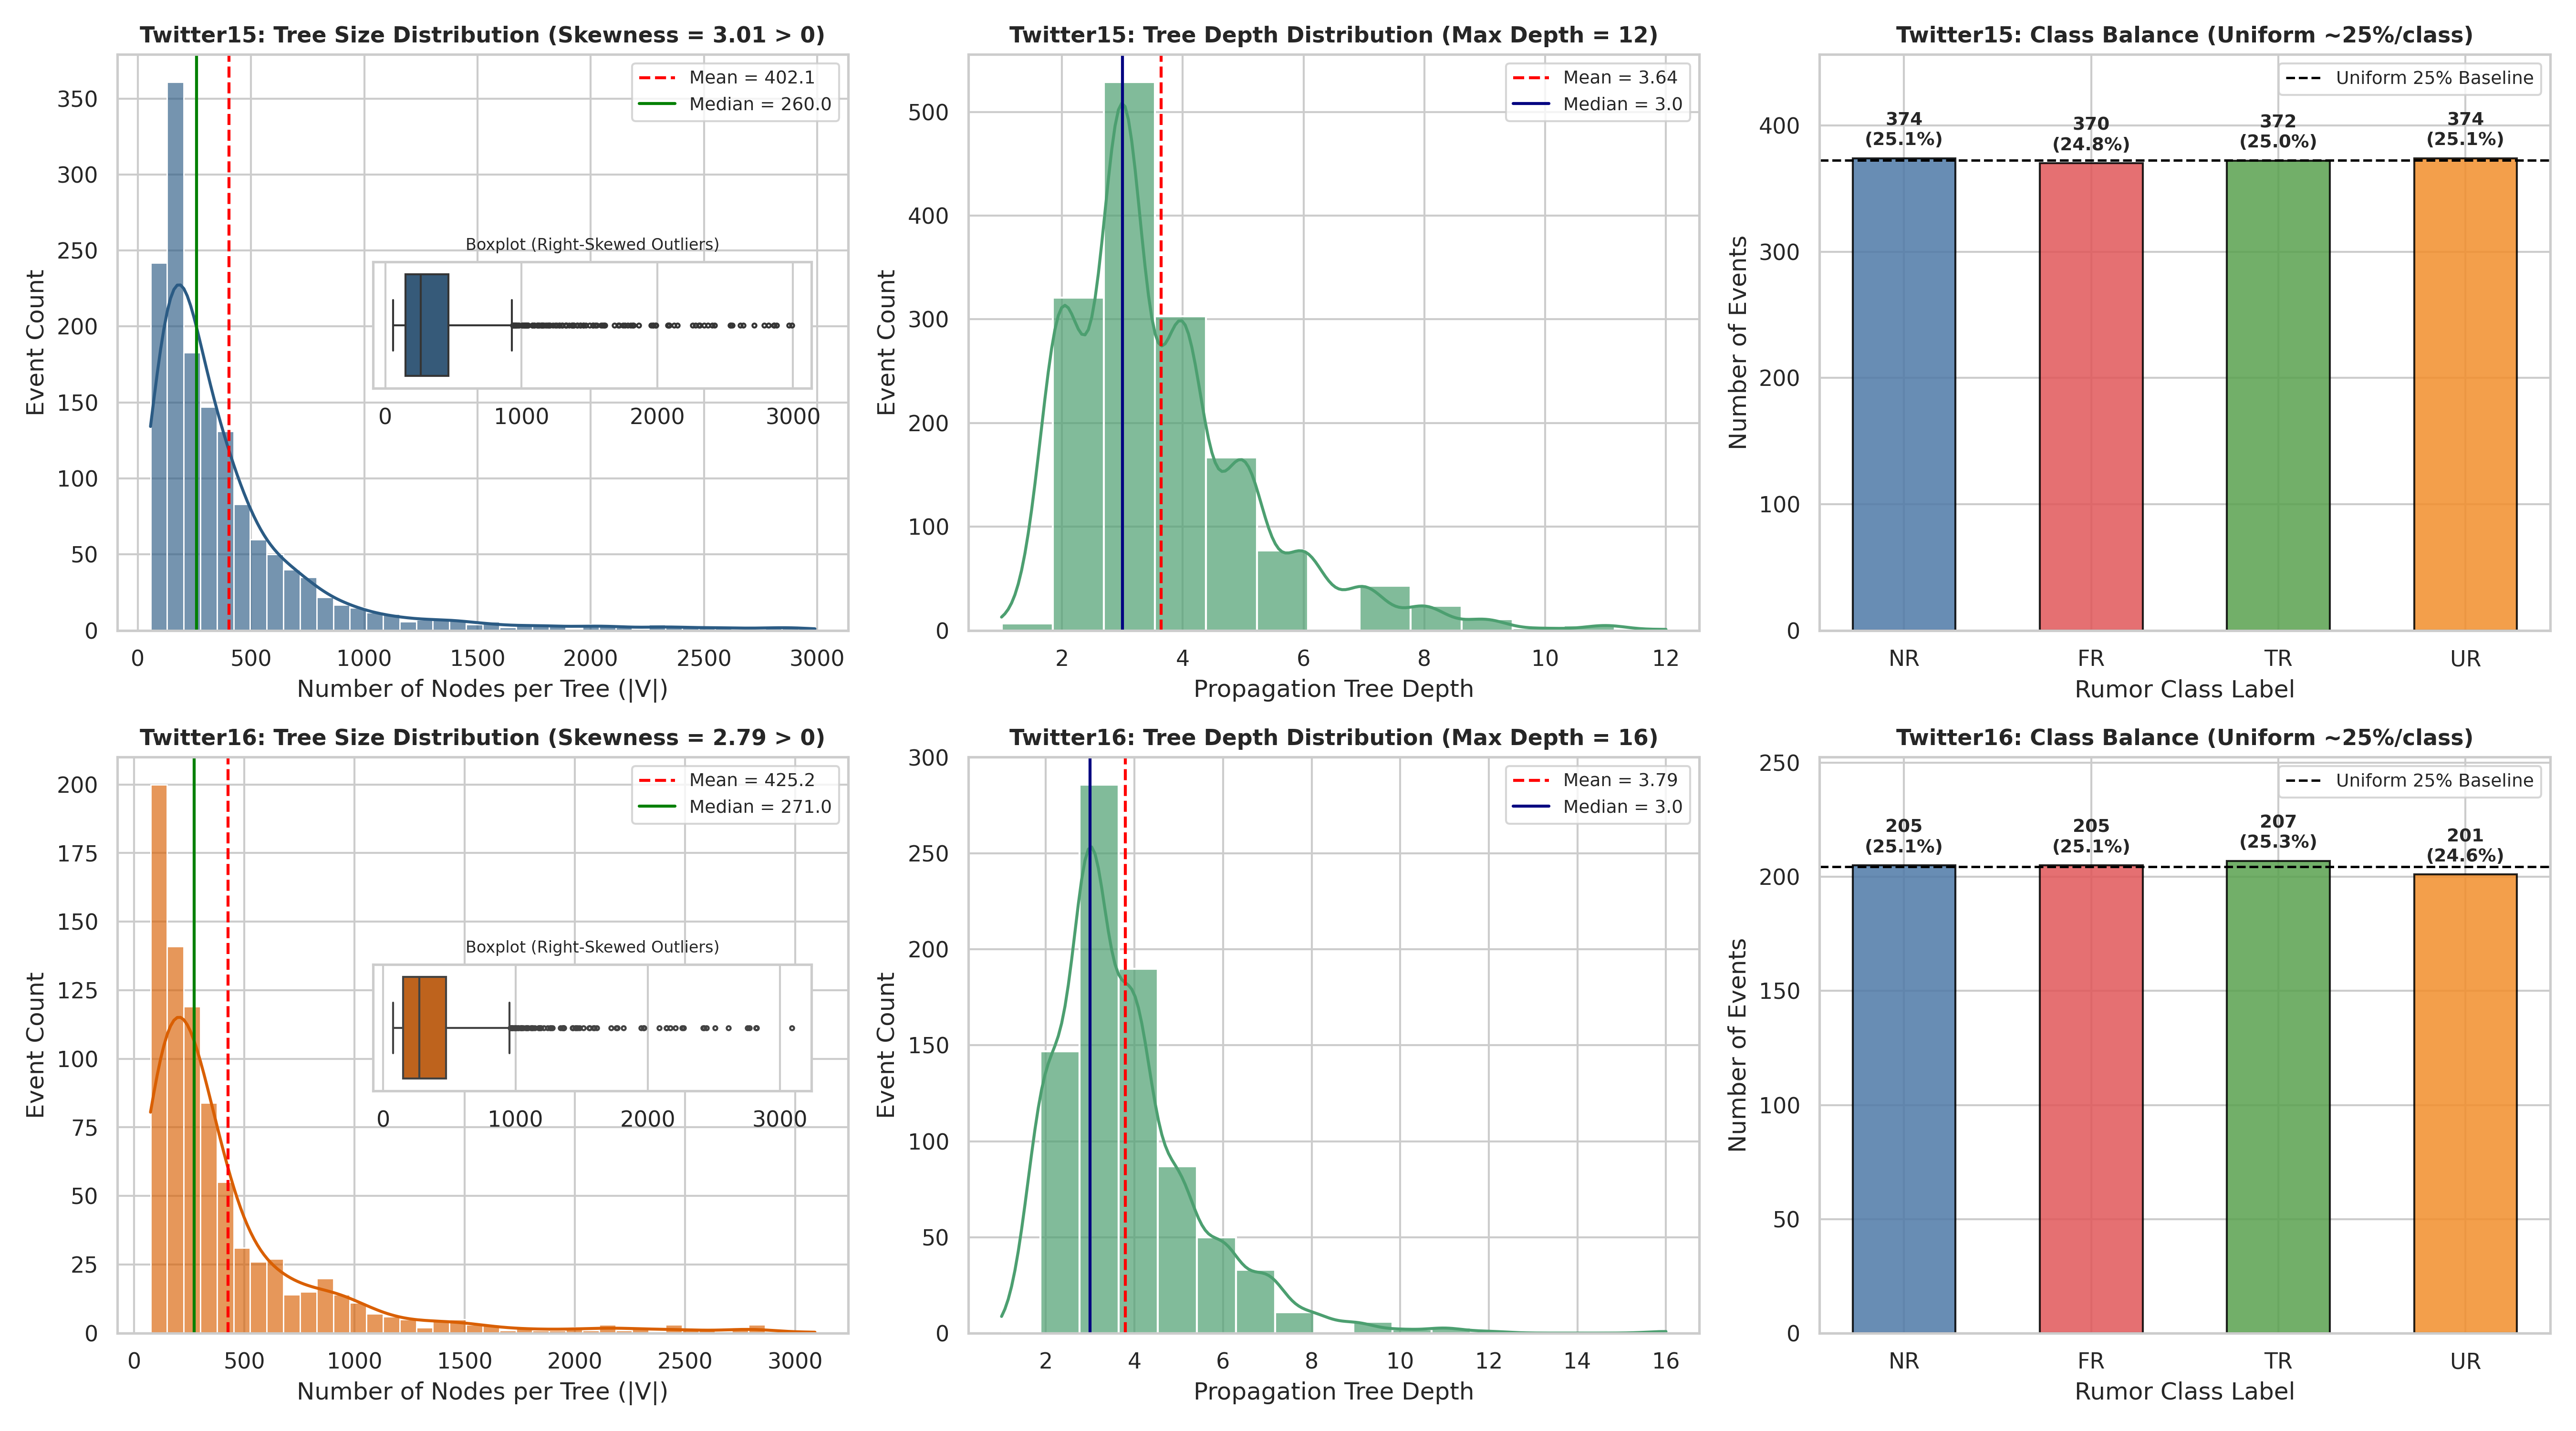
\includegraphics[width=0.96\textwidth]{figures/dataset_histogram.png}
    \caption{Biểu đồ Histogram phân bố kích thước cây, độ sâu cây lan truyền và tỷ lệ cân bằng bốn nhãn lớp trên Twitter15 ($N=1.490$) và Twitter16 ($N=818$)}
    \label{fig:dataset-histogram}
\end{figure}

\begin{figure}[htbp]
    \centering
    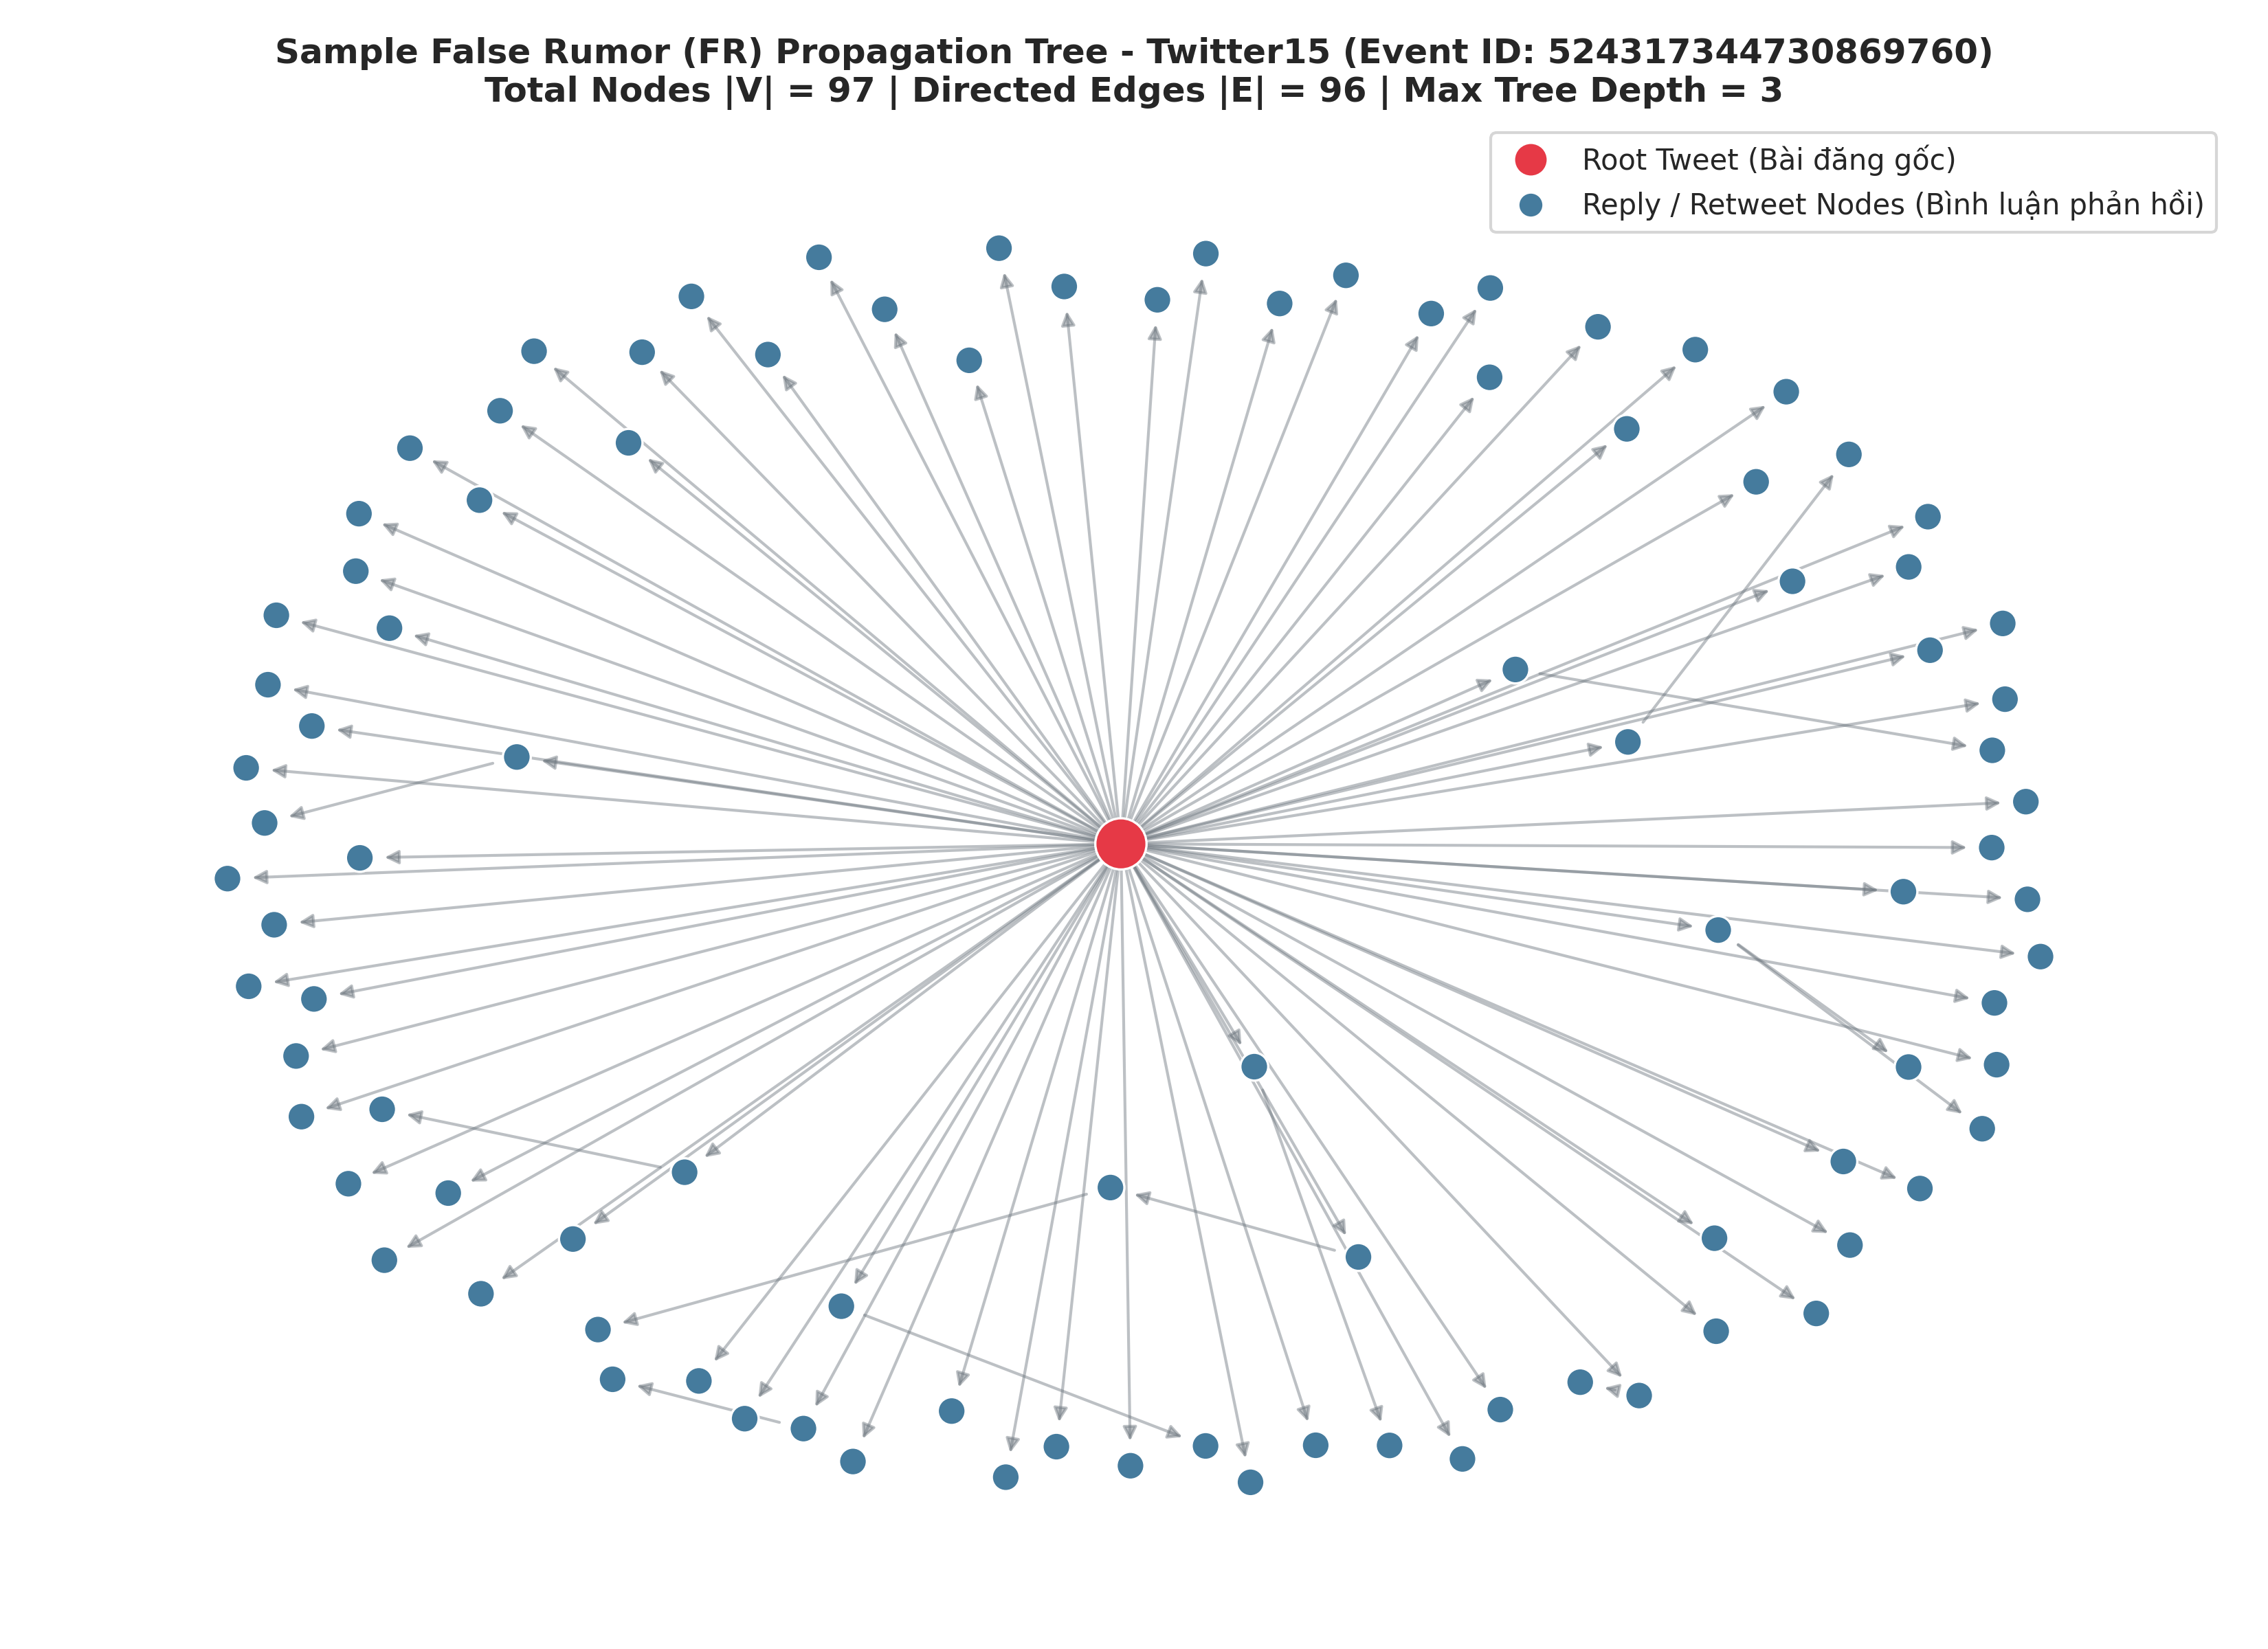
\includegraphics[width=0.72\textwidth]{figures/sample_event_visualization.png}
    \caption{Trực quan hóa một cây lan truyền tin giả mẫu (\textit{False Rumor}, ID: \texttt{524317344730869760}) trên Twitter15 gồm 97 nút và độ sâu tối đa 3 tầng}
    \label{fig:sample-event}
\end{figure}

\subsection{Khảo sát mã nguồn mở cơ sở và trực quan hóa quy trình xử lý (Pipeline)}

\subsubsection{1. Các kho mã nguồn mở cơ sở phục vụ nghiên cứu và thực nghiệm}
{\sloppy
Để phục vụ cho việc thiết kế mô hình và tái lập thực nghiệm, nhóm đã khảo sát, chọn lọc và thu thập 06 kho mã nguồn mở chính thống tương thích trực tiếp với bài toán kết hợp NLP -- GNN và bộ dữ liệu Twitter15 / Twitter16:
\begin{enumerate}
    \item \textbf{Bi-GCN (Bian et al., AAAI 2020):} \url{https://github.com/TianBian95/BiGCN}. Đây là kho mã nguồn nền tảng chuẩn mực nhất cài đặt mạng tích chập đồ thị hai chiều (\textit{Bi-directional Graph Convolutional Networks}) bằng \texttt{PyTorch} và \texttt{PyTorch-Geometric}. Kho lưu trữ này cung cấp sẵn trọn bộ dữ liệu cây lan truyền \textbf{Twitter15} và \textbf{Twitter16}, tích hợp kỹ thuật điều chuẩn \texttt{DropEdge}, hai nhánh \texttt{TDRumorGCN} (Top-Down) và \texttt{BURumorGCN} (Bottom-Up) cùng cơ chế nối tắt đặc trưng bài gốc (\textit{Root Feature Enhancement}).
    \item \textbf{RAGCL (Contrastive Learning on Bi-GCN, 2024):} \url{https://github.com/CcQunResearch/RAGCL}. Kho mã nguồn mở phát triển trực tiếp trên nền tảng Bi-GCN và bộ dữ liệu \textbf{Twitter15 / Twitter16}, tích hợp thêm cơ chế học tương phản đồ thị thích ứng (\textit{Region-Aware Graph Contrastive Learning}) để tăng cường độ bền vững trước nhiễu cấu trúc.
    \item \textbf{SoLM / PEP (Propagation-Enhanced Language Model, 2025) \cite{noauthor_enhancing_2025}:} \url{https://github.com/CcQunResearch/SoLM}. Kho mã nguồn kết hợp mô hình ngôn ngữ tiền huấn luyện với cấu trúc đồ thị lan truyền xã hội trên dữ liệu \textbf{Twitter15 và Twitter16}.
    \item \textbf{Rumor\_RvNN (Ma et al., ACL 2017/2018) \cite{ma_detect_2017}:} \url{https://github.com/majingCUHK/Rumor_RvNN}. Kho lưu trữ gốc của chính nhóm tác giả công bố bộ dữ liệu \textbf{Twitter15 và Twitter16}, bao gồm dữ liệu cây hội thoại thô (\texttt{tree/*.txt}), văn bản bài nguồn và mã nguồn mô hình mạng nơ-ron đệ quy cấu trúc cây (Top-Down / Bottom-Up RvNN).
    \item \textbf{GNN-FakeNews / UPFD (Dou et al., SIGIR 2021) \cite{noauthor_ensemble_2024, noauthor_co-attention_2025}:} \url{https://github.com/safe-graph/GNN-FakeNews}. Bộ khung benchmark chuẩn hóa của \texttt{PyTorch-Geometric} cài đặt mô-đun kết hợp đặc trưng văn bản (BERT, RoBERTa, Word2Vec) với các kiến trúc GNN kinh điển (\texttt{GCNConv}, \texttt{GATConv}, \texttt{SAGEConv}, \texttt{GINConv}).
    \item \textbf{Comparative Analysis of GNNs \& Transformers (Kuntur et al., 2024) \cite{noauthor_comparative_2024}:} \url{https://github.com/kunturs/comparative-analysis}. Kho mã nguồn đối sánh quy trình huấn luyện giữa nhóm mô hình GNN và nhóm mô hình Transformer.
\end{enumerate}

\par}

\subsubsection{2. Phân tích các bước thực hiện và Trực quan hóa quy trình (Pipeline)}
Thông qua việc giải phẫu cấu trúc mã nguồn của các kho lưu trữ trên (đặc biệt là \texttt{TianBian95/BiGCN} và \texttt{safe-graph/GNN-FakeNews}), quy trình hoạt động tổng thể của hệ thống phát hiện tin đồn kết hợp NLP và GNN hai chiều trên bộ dữ liệu Twitter15 và Twitter16 được đúc kết thành 5 giai đoạn và trực quan hóa tại Hình \ref{fig:pipeline}:

\begin{figure}[htbp]
    \centering
    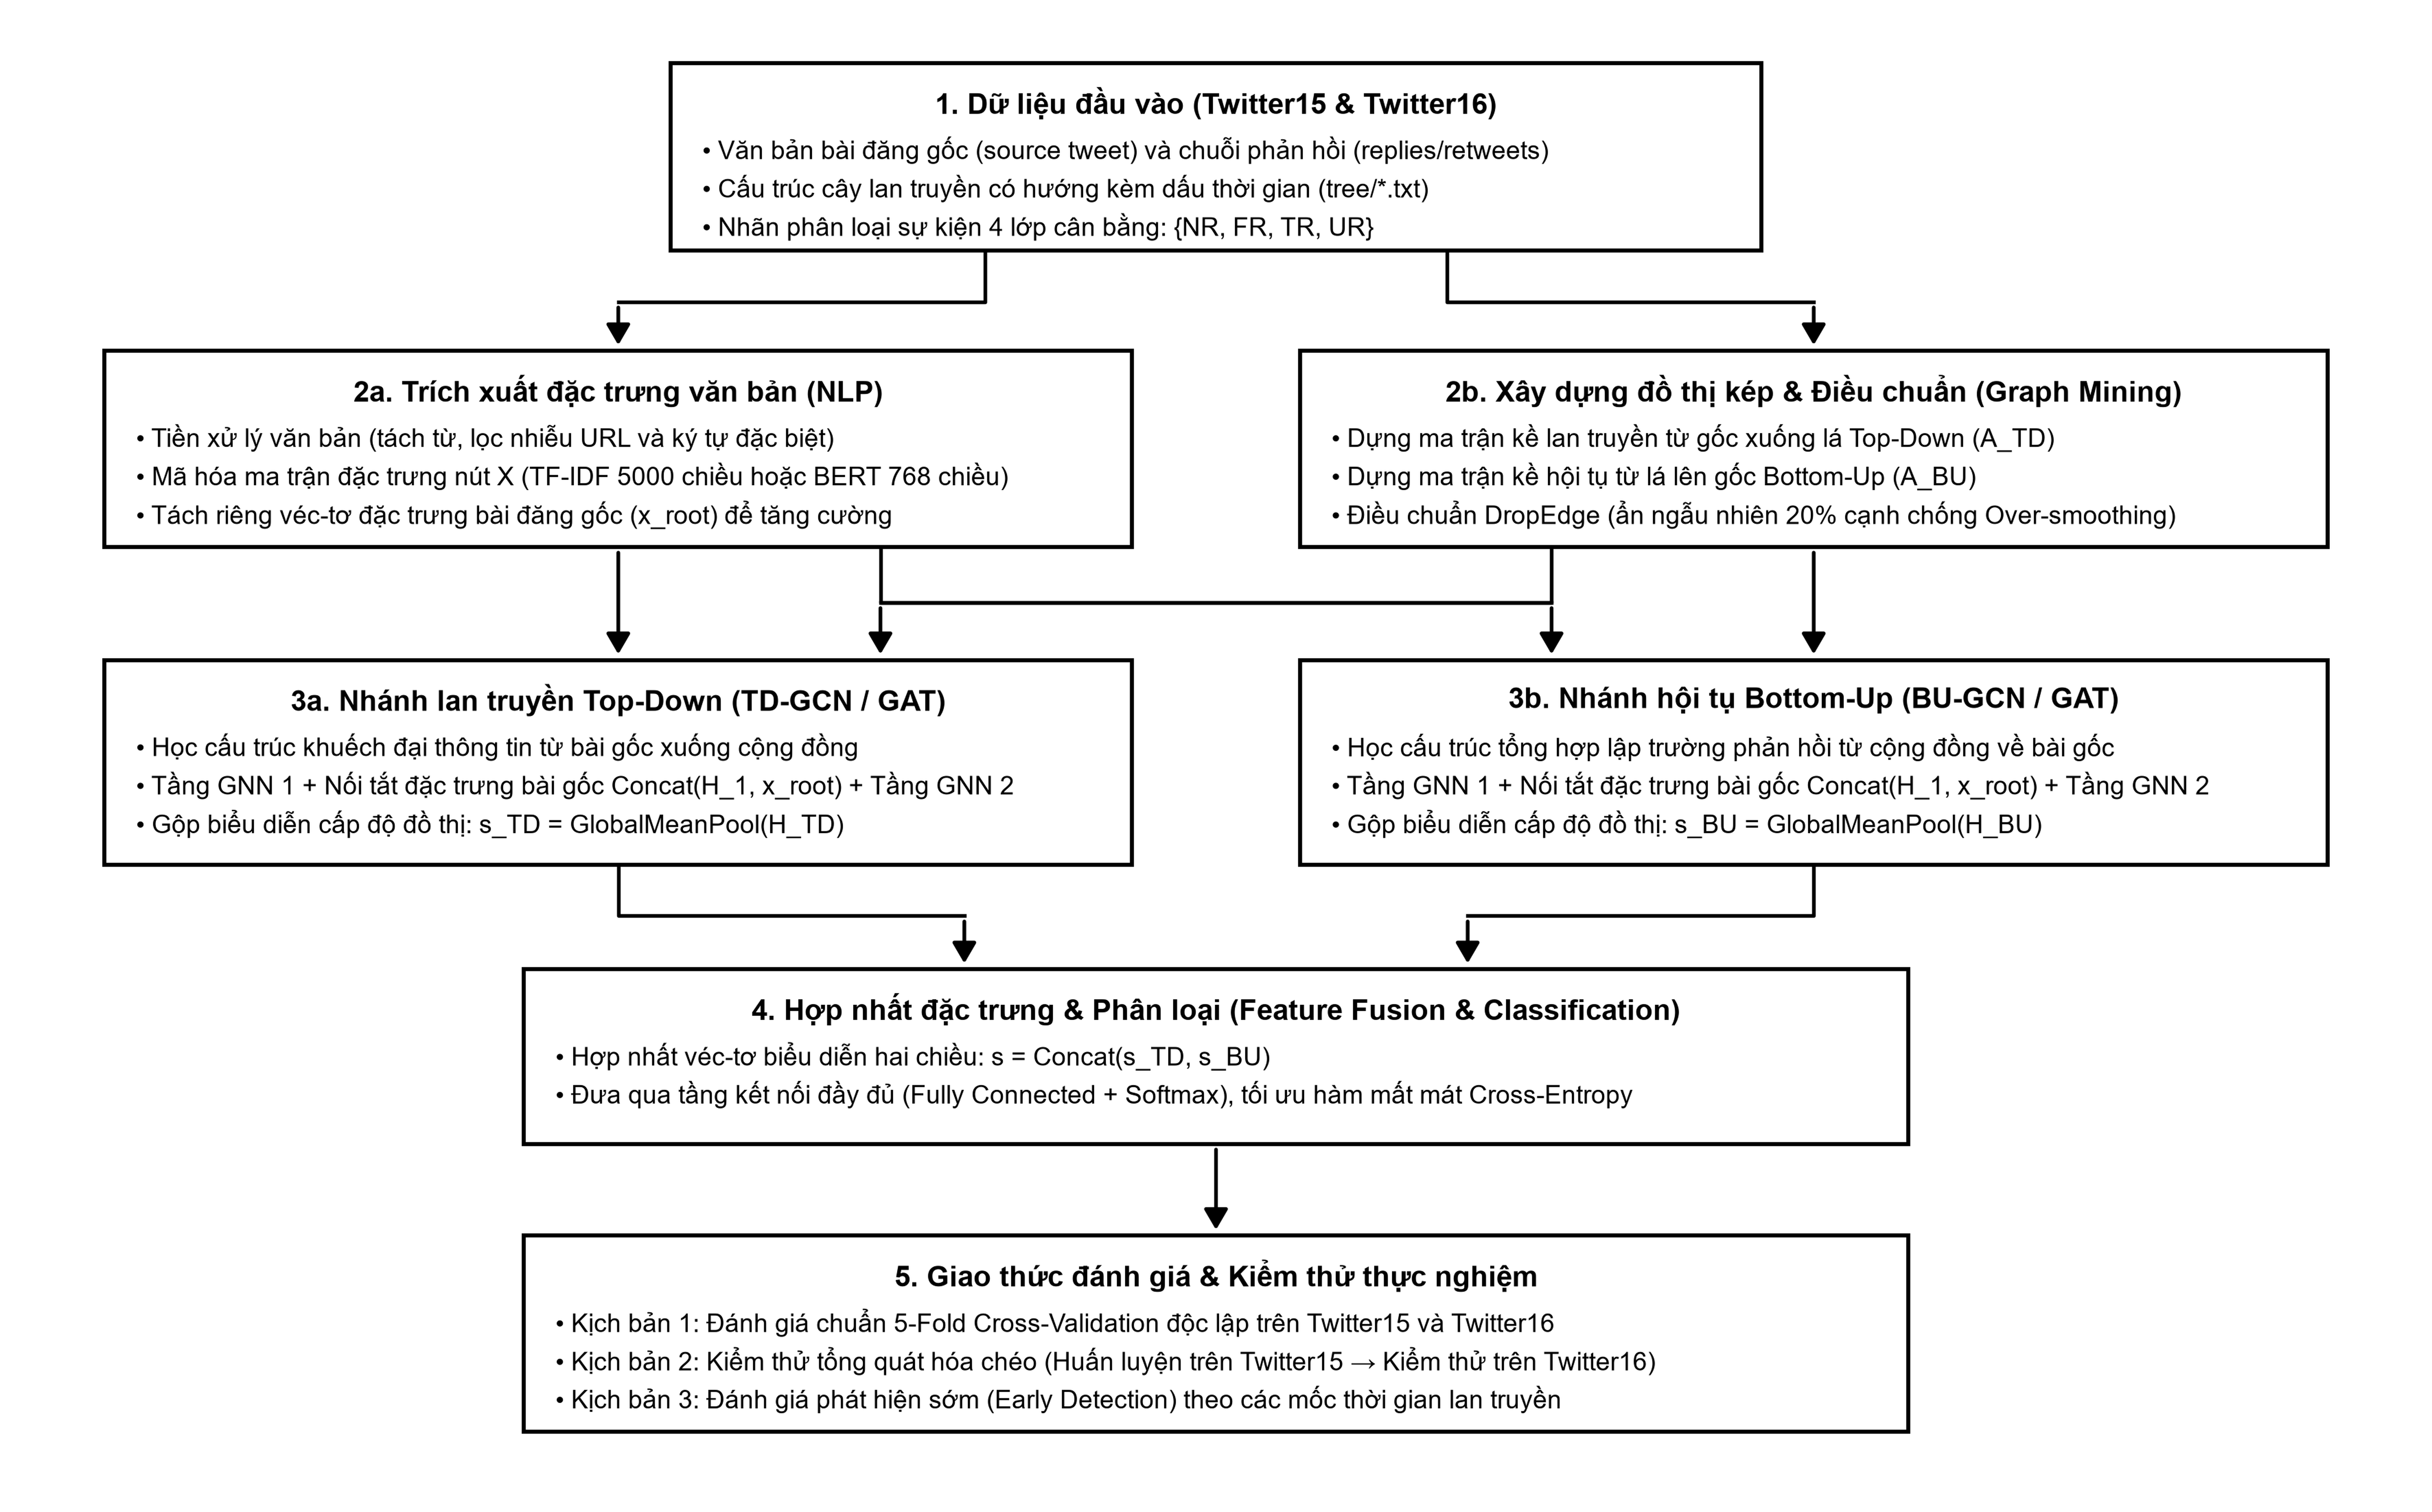
\includegraphics[width=0.96\textwidth]{pipeline.png}
    \caption[Sơ đồ quy trình (Pipeline) tổng thể kết hợp NLP và Bi-GCN / GAT]{Sơ đồ quy trình (Pipeline) tổng thể kết hợp trích xuất đặc trưng NLP và mạng tích chập đồ thị hai chiều (Bi-GCN / GAT) trên bộ dữ liệu Twitter15 và Twitter16 \coderef{report/pipeline.drawio}{Sơ đồ gốc}}
    \label{fig:pipeline}
\end{figure}

Cụ thể, từng giai đoạn trong quy trình tại Hình \ref{fig:pipeline} vận hành như sau:
\begin{itemize}
    \item \textbf{Giai đoạn 1 -- Thu nhận và đồng bộ dữ liệu đầu vào:} Hệ thống đọc dữ liệu sự kiện của Twitter15 và Twitter16 từ các tệp chuẩn hóa, bao gồm nhãn phân loại 4 lớp $\{NR, FR, TR, UR\}$, văn bản bài đăng gốc cùng các phản hồi và tệp cấu trúc cây hội thoại chứa cặp chỉ số \texttt{(nút cha $\rightarrow$ nút con)} theo trình tự thời gian lan truyền.
    \item \textbf{Giai đoạn 2 -- Trích xuất đặc trưng văn bản (NLP) và Xây dựng đồ thị kép (Graph Mining):}Ở nhánh NLP (2a), văn bản tại mỗi nút bài đăng được làm sạch và mã hóa thành ma trận đặc trưng nút $X \in \mathbb{R}^{|V| \times d}$ (sử dụng véc-tơ TF-IDF 5,000 chiều hoặc nhúng ngữ cảnh từ mô hình BERT 768 chiều), đồng thời tách riêng véc-tơ của bài đăng gốc $x_{\text{root}}$ để phục vụ cơ chế truyền tin nối tắt. Ở nhánh đồ thị (2b), từ một cây hội thoại ban đầu, hệ thống khởi tạo hai danh sách cạnh có hướng ngược nhau: ma trận kề lan truyền từ gốc xuống lá $A_{TD}$ (\textit{Top-Down}) và ma trận kề hội tụ từ lá lên gốc $A_{BU}$ (\textit{Bottom-Up}). Trong pha huấn luyện, kỹ thuật \texttt{DropEdge} được áp dụng để ngẫu nhiên loại bỏ một tỷ lệ cạnh ($p = 0.2$), giúp tăng tính đa dạng cấu trúc và ngăn chặn hiện tượng làm trơn quá mức (\textit{over-smoothing}).
    \item \textbf{Giai đoạn 3 -- Học biểu diễn đồ thị hai chiều và Tăng cường đặc trưng nút gốc:} Dữ liệu được đưa song song qua hai nhánh mạng nơ-ron đồ thị (có thể dùng tầng \texttt{GCNConv}, \texttt{GATConv} hoặc \texttt{SAGEConv}). Tại mỗi nhánh, sau khi đi qua tầng tích chập đồ thị thứ nhất ($H^{(1)}$), biểu diễn của mọi nút trong cây đều được ghép nối trực tiếp với đặc trưng của bài đăng gốc $\text{Concat}(H^{(1)}, x_{\text{root}})$ trước khi đi qua tầng tích chập thứ hai ($H^{(2)}$). Cơ chế này đảm bảo thông tin ngữ nghĩa của bài đăng nguồn không bị suy hao khi lan truyền qua nhiều bậc. Kết thúc giai đoạn 3, phép gộp trung bình toàn cục (\texttt{scatter\_mean} / \textit{Global Mean Pooling}) được thực hiện trên từng nhánh để thu được hai véc-tơ đại diện cấp độ đồ thị là $s_{TD}$ và $s_{BU}$.
    \item \textbf{Giai đoạn 4 -- Hợp nhất đặc trưng và Phân loại:} Hai véc-tơ biểu diễn luồng phát tán và luồng hội tụ được nối lại thành véc-tơ tổng hợp $s = \text{Concat}(s_{TD}, s_{BU})$, sau đó truyền qua tầng kết nối đầy đủ (\textit{Fully Connected Layer}) kèm hàm kích hoạt \texttt{Softmax} để dự đoán phân phối xác suất trên 4 lớp tin đồn. Mô hình được tối ưu hóa đầu-cuối bằng hàm mất mát Cross-Entropy và thuật toán Adam kèm điều chuẩn trọng số $L_2$.
    \item \textbf{Giai đoạn 5 -- Đánh giá và Kiểm thử theo 3 kịch bản:} Hệ thống xuất các chỉ số Accuracy, Precision, Recall và $F_1$-score cho từng lớp trên 3 kịch bản: (1) Đánh giá chéo 5-Fold Cross-Validation độc lập trên Twitter15 và Twitter16; (2) Kiểm thử khả năng tổng quát hóa chéo tập dữ liệu (huấn luyện trên Twitter15, kiểm thử trên Twitter16); và (3) Kiểm thử phát hiện sớm theo các mốc giới hạn thời gian lan truyền.
\end{itemize}


% =====================================================================
% CHƯƠNG 3: PHƯƠNG PHÁP ĐỀ XUẤT VÀ THIẾT KẾ THỰC NGHIỆM
% =====================================================================
\chapter{PHƯƠNG PHÁP ĐỀ XUẤT VÀ THIẾT KẾ THỰC NGHIỆM}

\section{Tiền xử lý dữ liệu và Biểu diễn đầu vào}

Do bộ dữ liệu công khai \texttt{rumdetect2017} (Twitter15 và Twitter16) \cite{ma_detect_2017} chỉ cung cấp nguyên văn bài đăng gốc (\texttt{source\_tweets.txt}) cùng cấu trúc cây phản hồi có dấu thời gian (\texttt{tree/*.txt}) mà không kèm nội dung bình luận của các nút con vì ràng buộc điều khoản nền tảng, việc biểu diễn đồng nhất toàn bộ nút bằng cùng một véc-tơ bài gốc sẽ làm mất tín hiệu cấu trúc địa phương. Để khắc phục, nhóm xây dựng quy trình tiền xử lý tách biệt hai loại thông tin cho mỗi cây lan truyền $G = (V, E)$:

\begin{itemize}
    \item \textbf{Đặc trưng từ vựng nút gốc (không rò rỉ dữ liệu kiểm thử):} Tại mỗi phân đoạn kiểm định chéo (fold), bộ trích xuất tần suất từ vựng \texttt{CountVectorizer} (tối đa $d_{\text{vocab}} = 5.000$ từ khóa phổ biến nhất) chỉ được khớp (\texttt{fit}) duy nhất trên tập huấn luyện (\textit{Train fold}, 80\% dữ liệu). Véc-tơ bài gốc $\mathbf{x}_{\text{text}} \in \mathbb{R}^{d_{\text{vocab}}}$ chỉ gắn tại nút gốc ($v = 0$), trong khi các nút phản hồi mang véc-tơ văn bản bằng $0$.
    \item \textbf{Đặc trưng cấu trúc và động lực thời gian nút:} Mỗi nút $v \in V$ (bao gồm cả nút gốc và các nút phản hồi) được gán một véc-tơ đặc trưng cấu trúc $\mathbf{s}_v \in \mathbb{R}^{5}$ cho các mô hình Cấp độ 1--2, gồm:
    \begin{equation}
        \mathbf{s}_v = \Big[\mathbb{I}(v=0),\; \frac{\ln(1+\Delta t_v)}{10},\; \ln(1+\text{depth}_v),\; \ln(1+\deg^+(v)),\; \frac{\text{order}_v}{\max(|V|-1,\,1)}\Big]^\top
        \label{eq:node-struct}
    \end{equation}
    trong đó $\Delta t_v \ge 0$ là độ trễ thời gian (phút) so với bài gốc, $\text{depth}_v$ là độ sâu từ gốc tính bằng BFS, $\deg^+(v)$ là số lượng phản hồi trực tiếp từ nút $v$, và $\text{order}_v$ là thứ tự xuất hiện theo thời gian đã chuẩn hóa về đoạn $[0, 1]$. Đối với kiến trúc đề xuất \texttt{BiGCN-Plus}, véc-tơ cấu trúc được mở rộng lên $8$ chiều ($\mathbf{s}_v^+ \in \mathbb{R}^8$) bằng cách bổ sung ba chiều gồm: cờ nút lá $\mathbb{I}(\deg^+(v)=0)$, kích thước cây con chuẩn hóa $\frac{\ln(1+\text{subtree}_v)}{\ln(1+|V|)}$, và độ trễ tương đối so với nút cha $\frac{\ln(1+\max(0, \Delta t_v - \Delta t_{\text{parent}(v)}))}{10}$.
\end{itemize}

\section{Các mô hình cơ sở và Biến thể giải phẫu (Cấp độ 1 \& Cấp độ 2)}

Nhằm đánh giá công bằng đóng góp của từng thành phần kiến trúc, nhóm thiết kế lộ trình thực nghiệm gồm ba cấp độ trên cùng một tập dữ liệu và tập chia 5-Fold:

\begin{enumerate}
    \item \textbf{Cấp độ 1 -- Các mô hình đối sánh cơ sở:}
    \begin{itemize}
        \item \texttt{MLP-BoW}: Mạng Perceptron đa tầng 2 lớp ẩn ($d'=64$) chỉ sử dụng véc-tơ văn bản $\mathbf{x}_{\text{text}}$ của bài đăng gốc, hoàn toàn bỏ qua cấu trúc cây lan truyền.
        \item \texttt{GCN-Single}: Mạng tích chập đồ thị 2 tầng trên đồ thị vô hướng $\tilde{\mathbf{A}} = \mathbf{A}_{TD} + \mathbf{A}_{TD}^\top + \mathbf{I}$, tổng hợp toàn đồ thị bằng phép gộp trung bình (\textit{Global Mean Pooling}).
        \item \texttt{GraphSAGE-Single}: Sử dụng cơ chế tách biệt trọng số nút trung tâm và trung bình láng giềng $\mathbf{h}_v^{(l)} = \sigma\big(\mathbf{W}_{\text{self}}\mathbf{h}_v^{(l-1)} + \mathbf{W}_{\text{neigh}}\cdot\text{mean}_{u\in\mathcal{N}(v)}(\mathbf{h}_u^{(l-1)})\big)$, giúp bảo toàn đặc trưng nút gốc khỏi hiện tượng pha loãng.
        \item \texttt{GAT-Single}: Mạng chú ý đồ thị với $K=4$ đầu chú ý ở tầng thứ nhất để gán trọng số động cho từng cạnh phản hồi.
    \end{itemize}
    \item \textbf{Cấp độ 2 -- Tái lập \texttt{BiGCN-Base} và 4 biến thể chuột bạch:}
    Kiến trúc \texttt{BiGCN-Base} (Bian và cộng sự, AAAI 2020) xử lý song song cây lan truyền theo hai hướng: nhánh xuôi Top-Down ($\mathbf{A}_{TD}$) và nhánh ngược Bottom-Up ($\mathbf{A}_{BU} = \mathbf{A}_{TD}^\top$). Tại mỗi nhánh, ma trận kề chuẩn hóa đối xứng có dạng:
    \begin{equation}
        \hat{\mathbf{A}}_d = \tilde{\mathbf{D}}_d^{-1/2}\big(\text{DropEdge}(\mathbf{A}_d, p_d) + \mathbf{I}\big)\tilde{\mathbf{D}}_d^{-1/2}, \quad d \in \{TD, BU\}
        \label{eq:bigcn-adj}
    \end{equation}
    Sau tầng tích chập thứ nhất $\mathbf{H}_d^{(1)} = \hat{\mathbf{A}}_d\mathbf{X}\mathbf{W}_d^{(1)}$, đặc trưng nút gốc $\mathbf{x}_{\text{root}}$ được ghép nối trực tiếp (\textit{Root Feature Enhancement}) trước khi qua tầng thứ hai và ghép thêm $\mathbf{h}_{d,\text{root}}^{(1)}$ sau phép gộp trung bình:
    \begin{equation}
        \mathbf{s}_d = \frac{1}{|V|}\sum_{v \in V} \Big[\text{ReLU}\big(\hat{\mathbf{A}}_d[\text{ReLU}(\mathbf{H}_d^{(1)}) \,\|\, \mathbf{X}_{\text{root}}]\mathbf{W}_d^{(2)}\big)_v \;\|\; \mathbf{h}_{d,\text{root}}^{(1)}\Big]
        \label{eq:bigcn-readout}
    \end{equation}
    Theo đúng cài đặt gốc của tác giả, các tầng tích chập ở nhánh Bottom-Up sử dụng tốc độ học vi phân $\eta_{BU} = \eta / 5$ nhằm ổn định gradient khi hội tụ từ nhiều nút lá về một nút gốc. Bốn biến thể giải phẫu (\textit{Ablation Study}) được thực nghiệm độc lập gồm: \texttt{BiGCN-NoRoot} (loại bỏ ghép nối nút gốc), \texttt{BiGCN-NoDropEdge} ($p_{TD}=p_{BU}=0$), \texttt{BiGCN-TDOnly} (chỉ giữ nhánh xuôi) và \texttt{BiGCN-BUOnly} (chỉ giữ nhánh ngược).
\end{enumerate}

\section{Kiến trúc đề xuất Cấp độ 3: \texttt{BiGCN-Plus} (V2)}

Trong thử nghiệm ban đầu (\texttt{BiGCN-Plus} V1), việc tăng trực tiếp chiều ẩn lên $128$, dùng $8.000$ chiều TF-IDF đưa thẳng vào các tầng GCN và bỏ tốc độ học vi phân $\eta/5$ đã đẩy số tham số lên $4{,}82$ triệu, dẫn đến quá khớp trên tập dữ liệu kích thước nhỏ ($654$ đồ thị huấn luyện ở mỗi fold của Twitter16) và làm độ chính xác giảm xuống $84{,}72\%$. Để khắc phục triệt để hạn chế này, nhóm đề xuất kiến trúc hợp nhất đa chuyên gia gọn nhẹ \textbf{\texttt{BiGCN-Plus} (V2)} (tổng tham số chỉ $0{,}99$ triệu trên Twitter16 và $1{,}56$ triệu trên Twitter15), kết hợp ba nhánh bổ trợ lẫn nhau:

\begin{enumerate}
    \item \textbf{Nhánh 1 -- Bộ mã hóa hai chiều chuẩn (\texttt{Exact BiGCN}):} Giữ nguyên cơ chế Top-Down + Bottom-Up với $d'=64$, DropEdge $p=0{,}2$, tốc độ học vi phân $\eta/5$ cho các tầng tích chập BU, nhưng nâng cấp đầu vào cấu trúc từ $5$ lên $8$ đặc trưng mở rộng ($\mathbf{s}_v^+$).
    \item \textbf{Nhánh 2 -- Bộ mã hóa song hướng không cắt cạnh (\texttt{Dual-View GraphSAGE}):} Hoạt động song song trên đồ thị giữ nguyên 100\% cạnh (\textit{NoDropEdge}, $d'=32$) với ma trận trọng số tách biệt cho nút tự thân ($\mathbf{W}_{\text{self}}$), láng giềng xuôi ($\mathbf{W}_{TD}$) và láng giềng ngược ($\mathbf{W}_{BU}$), kết hợp gộp trung bình toàn đồ thị với kết nối tắt hai tầng tại nút gốc $\mathbf{h}_{\text{root}}^{(2)} + \mathbf{h}_{\text{root}}^{(1)}$. Nhánh này đóng vai trò bảo vệ thông tin khi DropEdge ở Nhánh 1 vô tình cắt đứt các cạnh quan trọng gần gốc.
    \item \textbf{Nhánh 3 -- Đầu ngữ nghĩa tuyến tính dưới tuyến tính và Hồ sơ lan truyền (\texttt{Sublinear TF-IDF + LOO Hat-Matrix}):} Trích xuất biểu diễn văn bản TF-IDF dưới tuyến tính ($1 + \ln(\text{tf})$) trên cụm từ $(1,2)$-gram và chuỗi ký tự $(3,4)$-gram, kết hợp $10$ đặc trưng thống kê cấu trúc--thời gian cấp toàn đồ thị cho cấu hình chuẩn sạch \texttt{BiGCN-Plus-Clean} (hoàn toàn \textbf{không} sử dụng mã định danh tài khoản User-ID nhằm tránh rủi ro học thuộc tài khoản), đồng thời tách riêng biến thể đối chứng \texttt{BiGCN-Plus-UserID} (có ma trận nhân $K_u$ từ tần suất User-ID) để kiểm định ablation. Bộ trích xuất chỉ \texttt{fit} thuần túy trên tập Train của từng fold. Để ngăn chặn hoàn toàn nhánh tuyến tính học thuộc nhãn tập Train khi huấn luyện kết hợp, đầu ra của Nhánh 3 trên tập Train được tính qua ma trận mũ loại-một-ra (\textit{Leave-One-Out Hat Matrix}) chính xác:
    \begin{equation}
        \hat{\mathbf{y}}_i^{\text{LOO}} = \frac{\hat{\mathbf{y}}_i - H_{ii}\,\mathbf{y}_i}{1 - H_{ii}}, \quad \mathbf{H} = \mathbf{Z}(\mathbf{Z}^\top \mathbf{Z} + \lambda \mathbf{I})^{-1}\mathbf{Z}^\top
        \label{eq:loo-hat}
    \end{equation}
    trong đó $\mathbf{Z}$ là ma trận đặc trưng đã chuẩn hóa $L_2$ của tập huấn luyện.
    \item \textbf{Hợp nhất hiệu chỉnh và Trung bình pha cuối (\textit{Epoch-Tail Snapshot Ensembling}):} Ba luồng logit $\mathbf{o}_1, \mathbf{o}_2, \mathbf{o}_3$ được kết hợp bằng trọng số học được $\mathbf{w} = \text{softmax}(\boldsymbol{\alpha})$ dưới hàm mất mát đa nhiệm $\mathcal{L} = \mathcal{L}_{\text{fusion}} + 0{,}35\,\mathcal{L}_{\text{BiGCN}} + 0{,}25\,\mathcal{L}_{\text{SAGE}}$. Ở pha suy luận, mô hình lấy trung bình xác suất dự đoán của $K = 5$ epoch cuối cùng (epoch $96\text{--}100$) nhằm triệt tiêu phương sai dao động cuối kỳ mà hoàn toàn không dùng tập Test để chọn checkpoint. Trong bộ khung thực nghiệm chuẩn hóa (\texttt{CT255\_\-RumorDetection\_\-BiGCN\_Plus}), cơ chế đánh giá song song cả \texttt{Last Epoch} lẫn \texttt{Snapshot-5} được áp dụng đồng nhất cho mọi mô hình GNN (bao gồm \texttt{BiGCN-Base+}).
\end{enumerate}

Tổng thể luồng xử lý và cơ chế hợp nhất ba nhánh của kiến trúc đề xuất \texttt{BiGCN-Plus} được trực quan hóa bằng đồ họa vector tại Hình~\ref{fig:bigcn-plus-arch}. Cụ thể, dữ liệu đầu vào gồm bài đăng gốc ($\mathbf{x}_{\text{root}}$) và cây lan truyền hai chiều ($A_{TD}, A_{BU}$) kèm $8$ đặc trưng cấu trúc nút ($\mathbf{s}_v^+ \in \mathbb{R}^8$) được đưa đồng thời qua Nhánh 1 (\texttt{Exact BiGCN}) và Nhánh 2 (\texttt{Dual-View GraphSAGE}), trong khi đặc trưng văn bản \texttt{Sublinear TF-IDF} kết hợp $10$ thống kê đồ thị đi qua Nhánh 3 (\texttt{Kernel Ridge + LOO Hat Matrix}). Các luồng dự báo $\mathbf{o}_1, \mathbf{o}_2, \mathbf{o}_3$ sau đó được kết hợp qua tầng trọng số $\mathbf{w} = \text{softmax}(\boldsymbol{\alpha})$ và làm mượt bằng cơ chế \texttt{Snapshot-5} để xuất nhãn dự đoán cuối cùng trên $4$ lớp tin đồn.

\begin{figure}[htbp]
    \centering
    \begin{tikzpicture}[
        node distance=0.8cm and 0.9cm,
        box/.style={rectangle, draw=black, rounded corners=3pt, thick, align=center, font=\small, inner sep=6pt},
        inb/.style={box, fill=blue!8, minimum width=3.5cm, minimum height=1.15cm},
        brb/.style={box, fill=green!8, minimum width=4.4cm, minimum height=1.1cm},
        fusb/.style={box, fill=orange!12, minimum width=3.2cm, minimum height=1.25cm},
        outb/.style={box, fill=red!10, minimum width=2.7cm, minimum height=1.15cm},
        arr/.style={->, >=stealth, thick}
    ]
        \node[inb] (in1) {\textbf{Đầu vào Đồ thị}\\ $\mathbf{x}_{\text{root}}$ (BoW $5.000$)\\ $A_{TD}, A_{BU},\; \mathbf{s}_v^+ \in \mathbb{R}^8$};
        \node[inb, below=1.1cm of in1] (in2) {\textbf{Đầu vào Ngữ nghĩa}\\ Sublinear TF-IDF $(40\text{k})$\\ $+ 10$ thống kê đồ thị};

        \node[brb, right=1.0cm of in1, yshift=0.75cm] (b1) {\textbf{Nhánh 1: Exact BiGCN}\\ TD + BU, DropEdge ($p=0{,}2$)\\ $\eta_{BU} = \eta/5$, Root Skip $\rightarrow \mathbf{o}_1$};
        \node[brb, right=1.0cm of in1, yshift=-0.75cm] (b2) {\textbf{Nhánh 2: Dual-View SAGE}\\ NoDropEdge ($100\%$ cạnh)\\ $\mathbf{W}_{\text{self}}, \mathbf{W}_{TD}, \mathbf{W}_{BU} \rightarrow \mathbf{o}_2$};
        \node[brb, right=1.0cm of in2] (b3) {\textbf{Nhánh 3: Kernel Ridge}\\ LOO Hat Matrix $\mathbf{H}$ ($\lambda=0{,}45$)\\ Clean (không $K_u$) $\rightarrow \mathbf{o}_3$};

        \node[fusb, right=1.0cm of b2] (fus) {\textbf{Hợp nhất Softmax}\\ $\mathbf{w}=\text{softmax}(\boldsymbol{\alpha})$\\ $\sum_{k=1}^3 w_k \mathbf{o}_k$\\ + Snapshot-5};
        \node[outb, right=0.8cm of fus] (out) {\textbf{Dự đoán 4 lớp}\\ NR, FR,\\ TR, UR};

        \draw[arr] (in1.east) -- ++(0.35,0) |- (b1.west);
        \draw[arr] (in1.east) -- ++(0.35,0) |- (b2.west);
        \draw[arr] (in2.east) -- (b3.west);
        \draw[arr] (b1.east) -- ++(0.35,0) |- (fus.north west);
        \draw[arr] (b2.east) -- (fus.west);
        \draw[arr] (b3.east) -- ++(0.35,0) |- (fus.south west);
        \draw[arr] (fus.east) -- (out.west);
    \end{tikzpicture}
    \caption[Kiến trúc đề xuất BiGCN-Plus hợp nhất ba nhánh]{Sơ đồ kiến trúc đề xuất \texttt{BiGCN-Plus} kết hợp ba nhánh \texttt{Exact BiGCN} ($\mathbf{o}_1$), \texttt{Dual-View GraphSAGE} ($\mathbf{o}_2$) và \texttt{Kernel Ridge + LOO Hat Matrix} ($\mathbf{o}_3$) với tầng hợp nhất hiệu chỉnh $\mathbf{w}$ và \texttt{Snapshot-5} \coderef{src/bigcn_plus.py}{src/bigcn\_plus.py}}
    \label{fig:bigcn-plus-arch}
\end{figure}

\section{Thiết lập thực nghiệm, Độ phức tạp và Hệ thống 8 độ đo}

\subsection{Giao thức thực nghiệm và 5 quy tắc chuẩn hóa mã nguồn}
Trong đợt thực nghiệm ban đầu, toàn bộ 10 mô hình (4 Cấp 1, 5 Cấp 2, 1 Cấp 3) trên cả Twitter15 và Twitter16 được thực thi với bộ tham số thống nhất: \texttt{epochs = 100}, \texttt{batch\_size = 128}, \texttt{lr = 0.0005}, \texttt{weight\_decay = 1e-4}, \texttt{td\_droprate = bu\_droprate = 0.2}, cố định \texttt{seed = 42} (tức $1\text{ seed} \times 5\text{ folds} = 5$ lượt/mô hình) theo chuẩn \textbf{Stratified 5-Fold Cross-Validation} ($80\%$ Train -- $20\%$ Test ở mỗi fold, giữ nguyên thứ tự ID sắp xếp tăng dần). Nhằm khắc phục hạn chế của việc chạy đơn seed và bổ sung kiểm định ý nghĩa thống kê, nhóm đã xây dựng bộ mã nguồn mở rộng chuẩn hóa chạy mặc định \textbf{$5\text{ seeds} \times 5\text{ folds} = 25$ lượt/mô hình} (\texttt{seeds = [42..46]}) kèm kiểm định \textit{Paired t-test} và \textit{Wilcoxon signed-rank test}. Tập Test luôn ở trạng thái bất biến 100\% (\texttt{model.eval()}, \texttt{DropEdge = 0.0}). Mỗi lượt chạy tự động lưu các tệp minh chứng chuẩn 300~DPI gồm: \texttt{summary\_report.txt}, \texttt{epoch\_logs.csv}, \texttt{training\_curves.png} và \texttt{confusion\_matrix.png}.

\subsection{Công thức toán học của hệ thống 8 độ đo đánh giá}
Gọi $N$ là tổng số sự kiện kiểm thử, $C = 4$ là số phân lớp $\{NR, FR, TR, UR\}$, và $TP_c, FP_c, FN_c, TN_c$ lần lượt là số lượng dương tính thật, dương tính giả, âm tính giả và âm tính thật của lớp $c$. Hệ thống đánh giá toàn diện sử dụng 8 nhóm độ đo sau:

\begin{equation}
    \text{Accuracy} = \frac{1}{N}\sum_{c=1}^{C} TP_c
    \label{eq:acc}
\end{equation}

\begin{equation}
    \text{Macro-Precision} = \frac{1}{C}\sum_{c=1}^{C} \frac{TP_c}{TP_c + FP_c}, \qquad
    \text{Macro-Recall} = \frac{1}{C}\sum_{c=1}^{C} \frac{TP_c}{TP_c + FN_c}
    \label{eq:prec-rec}
\end{equation}

\begin{equation}
    F_{1,c} = \frac{2 \cdot P_c \cdot R_c}{P_c + R_c}, \qquad
    \text{Macro-}F_1 = \frac{1}{C}\sum_{c=1}^{C} F_{1,c}
    \label{eq:f1}
\end{equation}

\begin{equation}
    \kappa = \frac{p_o - p_e}{1 - p_e}, \quad \text{với } p_o = \text{Accuracy},\; p_e = \frac{1}{N^2}\sum_{c=1}^{C}(TP_c + FP_c)(TP_c + FN_c)
    \label{eq:kappa}
\end{equation}

\begin{equation}
    \text{MCC} = \frac{N\sum_{c} TP_c - \sum_{c} t_c p_c}{\sqrt{\big(N^2 - \sum_{c} p_c^2\big)\big(N^2 - \sum_{c} t_c^2\big)}}
    \label{eq:mcc}
\end{equation}
trong đó $t_c = TP_c + FN_c$ là tổng mẫu thực tế lớp $c$ và $p_c = TP_c + FP_c$ là tổng mẫu dự đoán lớp $c$. Cuối cùng, chỉ số phân biệt ngưỡng xác suất đa lớp \textbf{Macro OvR AUC-ROC} được tính bằng trung bình diện tích dưới đường cong ROC theo chiến lược một-chống-tất-cả:
\begin{equation}
    \text{AUC-ROC}_{\text{OvR}} = \frac{1}{C}\sum_{c=1}^{C} \int_0^1 \text{TPR}_c\big(\text{FPR}_c^{-1}(u)\big)\,du
    \label{eq:auc}
\end{equation}

\subsection{Độ phức tạp tính toán lý thuyết}
Gọi $|G|$ là số đồ thị, $|V|$ là tổng số nút, $|E|$ là tổng số cạnh, $d$ là số chiều đầu vào và $d'$ là chiều ẩn. Bảng~\ref{tab:complexity-theory} tổng hợp độ phức tạp tiệm cận theo từng kiến trúc khảo sát.

\begin{table}[htbp]
    \centering
    \caption{Độ phức tạp tính toán lý thuyết của các mô hình theo số đồ thị $|G|$, số nút $|V|$ và số cạnh $|E|$}
    \label{tab:complexity-theory}
    \small
    \begin{tabular}{@{}lll@{}}
        \toprule
        \textbf{Cấp độ} & \textbf{Mô hình} & \textbf{Độ phức tạp lý thuyết} \\
        \midrule
        Cấp 1 & \texttt{MLP-BoW} & $\mathcal{O}(|G|\cdot d\cdot d' + |G|\cdot d'^2)$ (không dùng đồ thị) \\
        Cấp 1 & \texttt{GCN-Single} & $\mathcal{O}(|V|\cdot d\cdot d' + |V|\cdot d'^2 + 2|E|\cdot d')$ \\
        Cấp 1 & \texttt{GraphSAGE-Single} & $\mathcal{O}(2|V|\cdot d\cdot d' + 2|V|\cdot d'^2 + 2|E|\cdot(d+d'))$ \\
        Cấp 1 & \texttt{GAT-Single} ($K=4$) & $\mathcal{O}(K|V|\cdot d\cdot d' + K|V|\cdot d'^2 + K|E|\cdot d')$ \\
        Cấp 2 & \texttt{BiGCN-Base} / \texttt{NoDropEdge} & $\mathcal{O}(2\cdot[|V|\cdot d\cdot d' + |V|\cdot(d+d')\cdot d' + 2|E|\cdot d'])$ \\
        Cấp 2 & \texttt{BiGCN-NoRoot} & $\mathcal{O}(2\cdot[|V|\cdot d\cdot d' + |V|\cdot d'^2 + 2|E|\cdot d'])$ \\
        Cấp 2 & \texttt{BiGCN-TDOnly} / \texttt{BUOnly} & $\mathcal{O}(|V|\cdot d\cdot d' + |V|\cdot(d+d')\cdot d' + 2|E|\cdot d')$ \\
        Cấp 3 & \texttt{BiGCN-Plus} (V2) & $\mathcal{O}(\text{BiGCN}) + \mathcal{O}(2|V|\cdot d\cdot d_{\text{sage}} + 4|E|\cdot d_{\text{sage}})$ \\
        \bottomrule
    \end{tabular}
\end{table}

% =====================================================================
% CHƯƠNG 4: KẾT QUẢ THỰC NGHIỆM
% =====================================================================
\chapter{KẾT QUẢ THỰC NGHIỆM}

Toàn bộ các kết quả thực nghiệm trong chương này được đo lường đồng nhất trên hạ tầng GPU Colab T4 (\texttt{cuda}) theo giao thức chuẩn hóa \textbf{$5\text{ seeds} \times 5\text{ folds} = 25$ lượt chạy độc lập} cho mỗi mô hình (tập hạt giống \texttt{seeds = [42, 43, 44, 45, 46]}, $100$ epoch/lượt). Tất cả các bảng số liệu tuân thủ nghiêm ngặt quy chuẩn bảng ba đường kẻ (\textit{Three-line table}), thống nhất dấu phân cách thập phân bằng dấu phẩy (,) cùng \textbf{đúng $5$ chữ số thập phân} ở mọi cột độ đo, căn phải toàn bộ cột số liệu, và cung cấp liên kết trực tiếp tới mã nguồn tái lập trên kho lưu trữ GitHub của nhóm.

\section{Kết quả các mô hình cơ sở Cấp độ 1 và Baseline NLP thuần văn bản}

Nhằm thiết lập chuẩn đối sánh rõ ràng giữa hiệu năng thuần văn bản và hiệu năng kết hợp cấu trúc đồ thị, nhóm đánh giá đồng thời ba mô hình NLP tuyến tính trên đặc trưng \texttt{Sublinear TF-IDF} (cụm từ $(1,2)$-gram và chuỗi ký tự $(3,4)$-gram, hoàn toàn không dùng đồ thị và không dùng User-ID) cùng bốn mô hình mạng nơ-ron Cấp độ 1 trên cả hai bộ dữ liệu. Kết quả trung bình qua $25$ lượt chạy được tổng hợp chi tiết tại Bảng~\ref{tab:nlp-multiseed} và Bảng~\ref{tab:level1-results}, từ đó rút ra ba nhận định quan trọng sau:

\begin{itemize}
    \item \textbf{Ngưỡng trần của tín hiệu văn bản bài gốc:} Như trình bày tại Bảng~\ref{tab:nlp-multiseed}, chỉ riêng mô hình tuyến tính \texttt{TF-IDF-Ridge} đạt độ chính xác trung bình $0{,}83691 \pm 0{,}01519$ trên Twitter15 (độ lệch chuẩn giữa các seed chỉ $0{,}00779$) và $0{,}85230 \pm 0{,}02954$ trên Twitter16 (Seed-Std là $0{,}00721$). Con số này vượt \texttt{MLP-BoW} tới $+0{,}01959$ trên Twitter15, khẳng định biểu diễn \texttt{Sublinear TF-IDF} kết hợp n-gram ký tự khai thác từ vựng bài đăng gốc hiệu quả hơn nhiều so với túi từ tần suất thô \texttt{CountVectorizer}.
    \item \textbf{Hiện tượng suy giảm của \texttt{GCN-Single} khi thiếu cơ chế bảo vệ nút gốc:} Theo Bảng~\ref{tab:level1-results}, \texttt{GCN-Single} chỉ đạt $0{,}77383$ trên Twitter15 và tụt sâu xuống $0{,}65356$ trên Twitter16 (thấp hơn mô hình thuần văn bản \texttt{MLP-BoW} tới $-0{,}19094$). Nguyên nhân xuất phát từ phép tích chập chuẩn hóa đối xứng qua $2$ tầng trên đồ thị vô hướng đã làm pha loãng véc-tơ từ vựng của bài đăng gốc bởi hàng trăm nút phản hồi mang véc-tơ văn bản rỗng, đặc biệt nghiêm trọng ở lớp \textit{False Rumor} ($F_1\text{-FR} = 0{,}47822$).
    \item \textbf{Lợi thế rõ rệt của \texttt{GraphSAGE-Single} nhờ tách biệt trọng số tự thân:} Nhờ sử dụng ma trận trọng số riêng $\mathbf{W}_{\text{self}}$ cho nút trung tâm tách biệt với trung bình láng giềng $\mathbf{W}_{\text{neigh}}$, \texttt{GraphSAGE-Single} dẫn đầu nhóm Cấp độ 1 trên cả Twitter15 ($0{,}83020$) và Twitter16 ($0{,}86137$), vượt \texttt{MLP-BoW} lần lượt $+0{,}01288$ và $+0{,}01687$ đồng thời đạt độ ổn định cao giữa các hạt giống (Seed-Std dưới $0{,}00465$).
\end{itemize}

\begin{table}[htbp]
    \centering
    \caption[Kết quả 25 lượt của nhóm Baseline NLP thuần văn bản]{Kết quả thực nghiệm $25$ lượt chạy ($5\text{ seeds} \times 5\text{ folds}$) cho nhóm Baseline NLP thuần văn bản (không đồ thị, không User-ID) trên GPU T4 \coderef{scripts/run_benchmark.py}{scripts/run\_benchmark.py}}
    \label{tab:nlp-multiseed}
    \footnotesize
    \setlength{\tabcolsep}{4pt}
    \begin{tabular}{@{}llrrrrrr@{}}
        \toprule
        \multicolumn{1}{c}{\textbf{Dataset}} & \multicolumn{1}{c}{\textbf{Mô hình}} & \multicolumn{1}{c}{\textbf{Accuracy (Mean $\pm$ Std)}} & \multicolumn{1}{c}{\textbf{Seed-Std}} & \multicolumn{1}{c}{\textbf{Macro-F1 (Mean $\pm$ Std)}} & \multicolumn{1}{c}{\textbf{Kappa}} & \multicolumn{1}{c}{\textbf{MCC}} & \multicolumn{1}{c}{\textbf{AUC-ROC}} \\
        \midrule
        Twitter15 & \texttt{TF-IDF-Ridge} & $\mathbf{0{,}83691 \pm 0{,}01519}$ & $0{,}00779$ & $\mathbf{0{,}83761 \pm 0{,}01511}$ & $\mathbf{0{,}78254}$ & $\mathbf{0{,}78346}$ & $\mathbf{0{,}95838}$ \\
        Twitter15 & \texttt{TF-IDF-LR}    & $0{,}83087 \pm 0{,}01630$ & $0{,}00902$ & $0{,}83265 \pm 0{,}01592$ & $0{,}77447$ & $0{,}77631$ & $0{,}95711$ \\
        Twitter15 & \texttt{TF-IDF-SVC}   & $0{,}79490 \pm 0{,}02574$ & $0{,}00948$ & $0{,}79168 \pm 0{,}02691$ & $0{,}72658$ & $0{,}72988$ & $0{,}94561$ \\
        \addlinespace[4pt]
        Twitter16 & \texttt{TF-IDF-Ridge} & $\mathbf{0{,}85230 \pm 0{,}02954}$ & $0{,}00721$ & $\mathbf{0{,}85304 \pm 0{,}02880}$ & $\mathbf{0{,}80306}$ & $\mathbf{0{,}80406}$ & $0{,}96446$ \\
        Twitter16 & \texttt{TF-IDF-LR}    & $0{,}84277 \pm 0{,}02640$ & $0{,}00598$ & $0{,}84483 \pm 0{,}02575$ & $0{,}79035$ & $0{,}79251$ & $\mathbf{0{,}96464}$ \\
        Twitter16 & \texttt{TF-IDF-SVC}   & $0{,}83422 \pm 0{,}02382$ & $0{,}00718$ & $0{,}83122 \pm 0{,}02406$ & $0{,}77899$ & $0{,}78167$ & $0{,}95630$ \\
        \bottomrule
    \end{tabular}
    \par\vspace{3pt}
    {\footnotesize\textit{Ghi chú: Các giá trị \textbf{in đậm} biểu thị kết quả cao nhất theo từng cột trên mỗi tập dữ liệu (đều đo ở chế độ đánh giá chuẩn qua $25$ lượt chạy).}}
\end{table}

\begin{table}[htbp]
    \centering
    \caption[Kết quả 25 lượt của 4 mô hình cơ sở Cấp độ 1]{Kết quả thực nghiệm $25$ lượt chạy ($5\text{ seeds} \times 5\text{ folds}$) của các mô hình Cấp độ 1 trên Twitter15 và Twitter16 \coderef{scripts/run_benchmark.py}{scripts/run\_benchmark.py}}
    \label{tab:level1-results}
    \footnotesize
    \setlength{\tabcolsep}{4pt}
    \begin{tabular}{@{}llrrrrrr@{}}
        \toprule
        \multicolumn{1}{c}{\textbf{Dataset}} & \multicolumn{1}{c}{\textbf{Mô hình}} & \multicolumn{1}{c}{\textbf{Accuracy (Mean $\pm$ Std)}} & \multicolumn{1}{c}{\textbf{Seed-Std}} & \multicolumn{1}{c}{\textbf{Macro-F1 (Mean $\pm$ Std)}} & \multicolumn{1}{c}{\textbf{Kappa}} & \multicolumn{1}{c}{\textbf{MCC}} & \multicolumn{1}{c}{\textbf{AUC-ROC}} \\
        \midrule
        Twitter15 & \texttt{MLP-BoW}          & $0{,}81732 \pm 0{,}02162$ & $0{,}00828$ & $0{,}81735 \pm 0{,}02148$ & $0{,}75642$ & $0{,}75729$ & $0{,}95865$ \\
        Twitter15 & \texttt{GCN-Single}       & $0{,}77383 \pm 0{,}02105$ & $0{,}00591$ & $0{,}77417 \pm 0{,}02079$ & $0{,}69842$ & $0{,}69985$ & $0{,}93268$ \\
        Twitter15 & \texttt{GAT-Single}       & $0{,}80228 \pm 0{,}02515$ & $0{,}00364$ & $0{,}80296 \pm 0{,}02505$ & $0{,}73636$ & $0{,}73829$ & $0{,}94819$ \\
        Twitter15 & \texttt{GraphSAGE-Single} & $\mathbf{0{,}83020 \pm 0{,}02603}$ & $0{,}00465$ & $\mathbf{0{,}83034 \pm 0{,}02593}$ & $\mathbf{0{,}77359}$ & $\mathbf{0{,}77437}$ & $\mathbf{0{,}96105}$ \\
        \addlinespace[4pt]
        Twitter16 & \texttt{MLP-BoW}          & $0{,}84450 \pm 0{,}02257$ & $0{,}01037$ & $0{,}84437 \pm 0{,}02267$ & $0{,}79265$ & $0{,}79368$ & $0{,}96907$ \\
        Twitter16 & \texttt{GCN-Single}       & $0{,}65356 \pm 0{,}03560$ & $0{,}01267$ & $0{,}64670 \pm 0{,}03698$ & $0{,}53800$ & $0{,}54330$ & $0{,}87422$ \\
        Twitter16 & \texttt{GAT-Single}       & $0{,}84206 \pm 0{,}02723$ & $0{,}00420$ & $0{,}84347 \pm 0{,}02701$ & $0{,}78937$ & $0{,}79194$ & $0{,}96440$ \\
        Twitter16 & \texttt{GraphSAGE-Single} & $\mathbf{0{,}86137 \pm 0{,}02489}$ & $0{,}00393$ & $\mathbf{0{,}86122 \pm 0{,}02524}$ & $\mathbf{0{,}81514}$ & $\mathbf{0{,}81645}$ & $\mathbf{0{,}97170}$ \\
        \bottomrule
    \end{tabular}
    \par\vspace{3pt}
    {\footnotesize\textit{Ghi chú: Các giá trị \textbf{in đậm} biểu thị kết quả cao nhất trong nhóm Cấp độ 1 trên từng tập dữ liệu (chế độ đánh giá \texttt{last}, epoch $100$).}}
\end{table}

\section{Đánh giá nhóm Cấp độ 2: \texttt{BiGCN-Base}, Biến thể giải phẫu và GNN hậu-2020}

Để phân tách vai trò của từng cơ chế trong mạng tích chập đồ thị hai chiều đồng thời đối chiếu với các kiến trúc GNN hiện đại sau năm 2020, nhóm thực hiện $25$ lượt chạy cho \texttt{BiGCN-Base}, bốn biến thể giải phẫu (\texttt{BiGCN-NoDropEdge}, \texttt{BiGCN-TDOnly}, \texttt{BiGCN-NoRoot}, \texttt{BiGCN-BUOnly}) cùng hai mô hình đối chứng \texttt{EBGCN} (ACL 2021) \cite{wei_towards_2021} và \texttt{RAGCL} (AAAI 2024) \cite{cui_propagation_2024}. Kết quả định lượng chi tiết được trình bày tại Bảng~\ref{tab:ablation-results} và minh họa trực quan tại Hình~\ref{fig:ablation}, cho thấy ba kết luận thực nghiệm nổi bật:

\begin{itemize}
    \item \textbf{Tác động quyết định của nhánh Top-Down và tăng cường đặc trưng nút gốc:} Khi loại bỏ hoàn toàn nhánh lan truyền xuôi (\texttt{BiGCN-BUOnly}), hiệu năng sụt giảm đặc biệt nghiêm trọng trên cả Twitter15 ($0{,}47530$, giảm $-0{,}35960$ so với \texttt{BiGCN-Base}) và Twitter16 ($0{,}50612$, giảm $-0{,}30733$), do trên tập mở thiếu văn bản phản hồi, luồng ngược từ lá về gốc không thể lan truyền ngữ nghĩa bài nguồn xuống các nút con. Tương tự, việc tắt cơ chế tăng cường đặc trưng nút gốc (\texttt{BiGCN-NoRoot}) làm giảm $-0{,}06859$ trên Twitter15 (xuống $0{,}76631$) và $-0{,}09974$ trên Twitter16 (xuống $0{,}71371$).
    \item \textbf{Sự ổn định của nhánh xuôi và cơ chế điều chuẩn DropEdge:} Biến thể \texttt{BiGCN-NoDropEdge} đạt $0{,}83530$ (Twitter15) và $0{,}81688$ (Twitter16), gần như tương đương \texttt{BiGCN-Base} ($0{,}83490$ và $0{,}81345$) với sai khác không có ý nghĩa thống kê ($p = 0{,}56010$ trên Twitter15), cho thấy trên đồ thị cây có kích thước vừa phải và $5$ đặc trưng cấu trúc gọn nhẹ, \texttt{DropEdge} giúp giảm nhẹ phương sai nhưng không làm thay đổi đáng kể điểm trung bình.
    \item \textbf{Hiệu năng của các baseline GNN hậu-2020 trên tập mở:} Mô hình \texttt{EBGCN} đạt hiệu năng rất tốt trên Twitter16 ($0{,}85478 \pm 0{,}02339$, AUC-ROC $0{,}97251$) nhờ cơ chế cổng trọng số cạnh Bayesian lọc bớt các cạnh phản hồi nhiễu, trong khi \texttt{RAGCL} đạt $0{,}83007$ (Twitter15) và $0{,}79977$ (Twitter16) do mất mát tương phản đồ thị bị hạn chế khi các nút con thiếu văn bản bình luận gốc.
\end{itemize}

\begin{table}[htbp]
    \centering
    \caption[Kết quả 25 lượt của nhóm BiGCN Ablation, EBGCN và RAGCL]{Kết quả thực nghiệm $25$ lượt chạy của \texttt{BiGCN-Base}, $4$ biến thể giải phẫu (Ablation Study) cùng các baseline \texttt{EBGCN} và \texttt{RAGCL} \coderef{scripts/CT255_RumorDetection_BiGCN_Plus_MultiSeed_5x5_Colab_T4GPU.ipynb}{Colab Cell 3--4}}
    \label{tab:ablation-results}
    \footnotesize
    \setlength{\tabcolsep}{4pt}
    \begin{tabular}{@{}llrrrrrr@{}}
        \toprule
        \multicolumn{1}{c}{\textbf{Dataset}} & \multicolumn{1}{c}{\textbf{Mô hình / Biến thể}} & \multicolumn{1}{c}{\textbf{Accuracy (Mean $\pm$ Std)}} & \multicolumn{1}{c}{\textbf{Macro-F1 (Mean $\pm$ Std)}} & \multicolumn{1}{c}{\textbf{$\Delta$Acc vs Base}} & \multicolumn{1}{c}{\textbf{Kappa}} & \multicolumn{1}{c}{\textbf{MCC}} & \multicolumn{1}{c}{\textbf{AUC-ROC}} \\
        \midrule
        Twitter15 & \texttt{BiGCN-Base}       & $0{,}83490 \pm 0{,}01943$ & $0{,}83509 \pm 0{,}01926$ & $0{,}00000$ & $0{,}77985$ & $0{,}78087$ & $0{,}95878$ \\
        Twitter15 & \texttt{BiGCN-NoDropEdge} & $\mathbf{0{,}83530 \pm 0{,}02329}$ & $\mathbf{0{,}83548 \pm 0{,}02317}$ & $+0{,}00040$ & $\mathbf{0{,}78037}$ & $\mathbf{0{,}78247}$ & $0{,}95915$ \\
        Twitter15 & \texttt{BiGCN-TDOnly}     & $0{,}81356 \pm 0{,}02254$ & $0{,}81330 \pm 0{,}02238$ & $-0{,}02134$ & $0{,}75142$ & $0{,}75462$ & $0{,}95605$ \\
        Twitter15 & \texttt{BiGCN-NoRoot}     & $0{,}76631 \pm 0{,}02015$ & $0{,}76614 \pm 0{,}02094$ & $-0{,}06859$ & $0{,}68840$ & $0{,}69359$ & $0{,}93831$ \\
        Twitter15 & \texttt{BiGCN-BUOnly}     & $0{,}47530 \pm 0{,}02714$ & $0{,}45379 \pm 0{,}03049$ & $-0{,}35960$ & $0{,}30017$ & $0{,}30846$ & $0{,}73985$ \\
        Twitter15 & \texttt{EBGCN} (ACL 2021) & $0{,}83154 \pm 0{,}01821$ & $0{,}83125 \pm 0{,}01827$ & $-0{,}00336$ & $0{,}77541$ & $0{,}77720$ & $\mathbf{0{,}96503}$ \\
        Twitter15 & \texttt{RAGCL} (AAAI 2024)& $0{,}83007 \pm 0{,}02460$ & $0{,}83019 \pm 0{,}02440$ & $-0{,}00483$ & $0{,}77340$ & $0{,}77505$ & $0{,}95541$ \\
        \addlinespace[4pt]
        Twitter16 & \texttt{BiGCN-Base}       & $0{,}81345 \pm 0{,}02766$ & $0{,}81428 \pm 0{,}02716$ & $0{,}00000$ & $0{,}75125$ & $0{,}75361$ & $0{,}95426$ \\
        Twitter16 & \texttt{BiGCN-NoDropEdge} & $0{,}81688 \pm 0{,}02394$ & $0{,}81750 \pm 0{,}02346$ & $+0{,}00343$ & $0{,}75580$ & $0{,}75777$ & $0{,}95676$ \\
        Twitter16 & \texttt{BiGCN-TDOnly}     & $0{,}83058 \pm 0{,}02189$ & $0{,}83016 \pm 0{,}02245$ & $+0{,}01713$ & $0{,}77409$ & $0{,}77586$ & $0{,}96247$ \\
        Twitter16 & \texttt{BiGCN-NoRoot}     & $0{,}71371 \pm 0{,}03880$ & $0{,}71192 \pm 0{,}03928$ & $-0{,}09974$ & $0{,}61830$ & $0{,}62354$ & $0{,}92021$ \\
        Twitter16 & \texttt{BiGCN-BUOnly}     & $0{,}50612 \pm 0{,}03886$ & $0{,}47699 \pm 0{,}04476$ & $-0{,}30733$ & $0{,}34101$ & $0{,}35129$ & $0{,}78244$ \\
        Twitter16 & \texttt{EBGCN} (ACL 2021) & $\mathbf{0{,}85478 \pm 0{,}02339}$ & $\mathbf{0{,}85479 \pm 0{,}02356}$ & $+0{,}04133$ & $\mathbf{0{,}80636}$ & $\mathbf{0{,}80766}$ & $\mathbf{0{,}97251}$ \\
        Twitter16 & \texttt{RAGCL} (AAAI 2024)& $0{,}79977 \pm 0{,}02853$ & $0{,}80103 \pm 0{,}02806$ & $-0{,}01368$ & $0{,}73298$ & $0{,}73522$ & $0{,}94619$ \\
        \bottomrule
    \end{tabular}
    \par\vspace{3pt}
    {\footnotesize\textit{Ghi chú: Giá trị \textbf{in đậm} thể hiện hiệu năng cao nhất trong nhóm Cấp độ 2 trên từng bộ dữ liệu; $\Delta\text{Acc vs Base} = \text{Acc}_{\text{mô hình}} - \text{Acc}_{\text{BiGCN-Base}}$.}}
\end{table}

\begin{figure}[htbp]
    \centering
    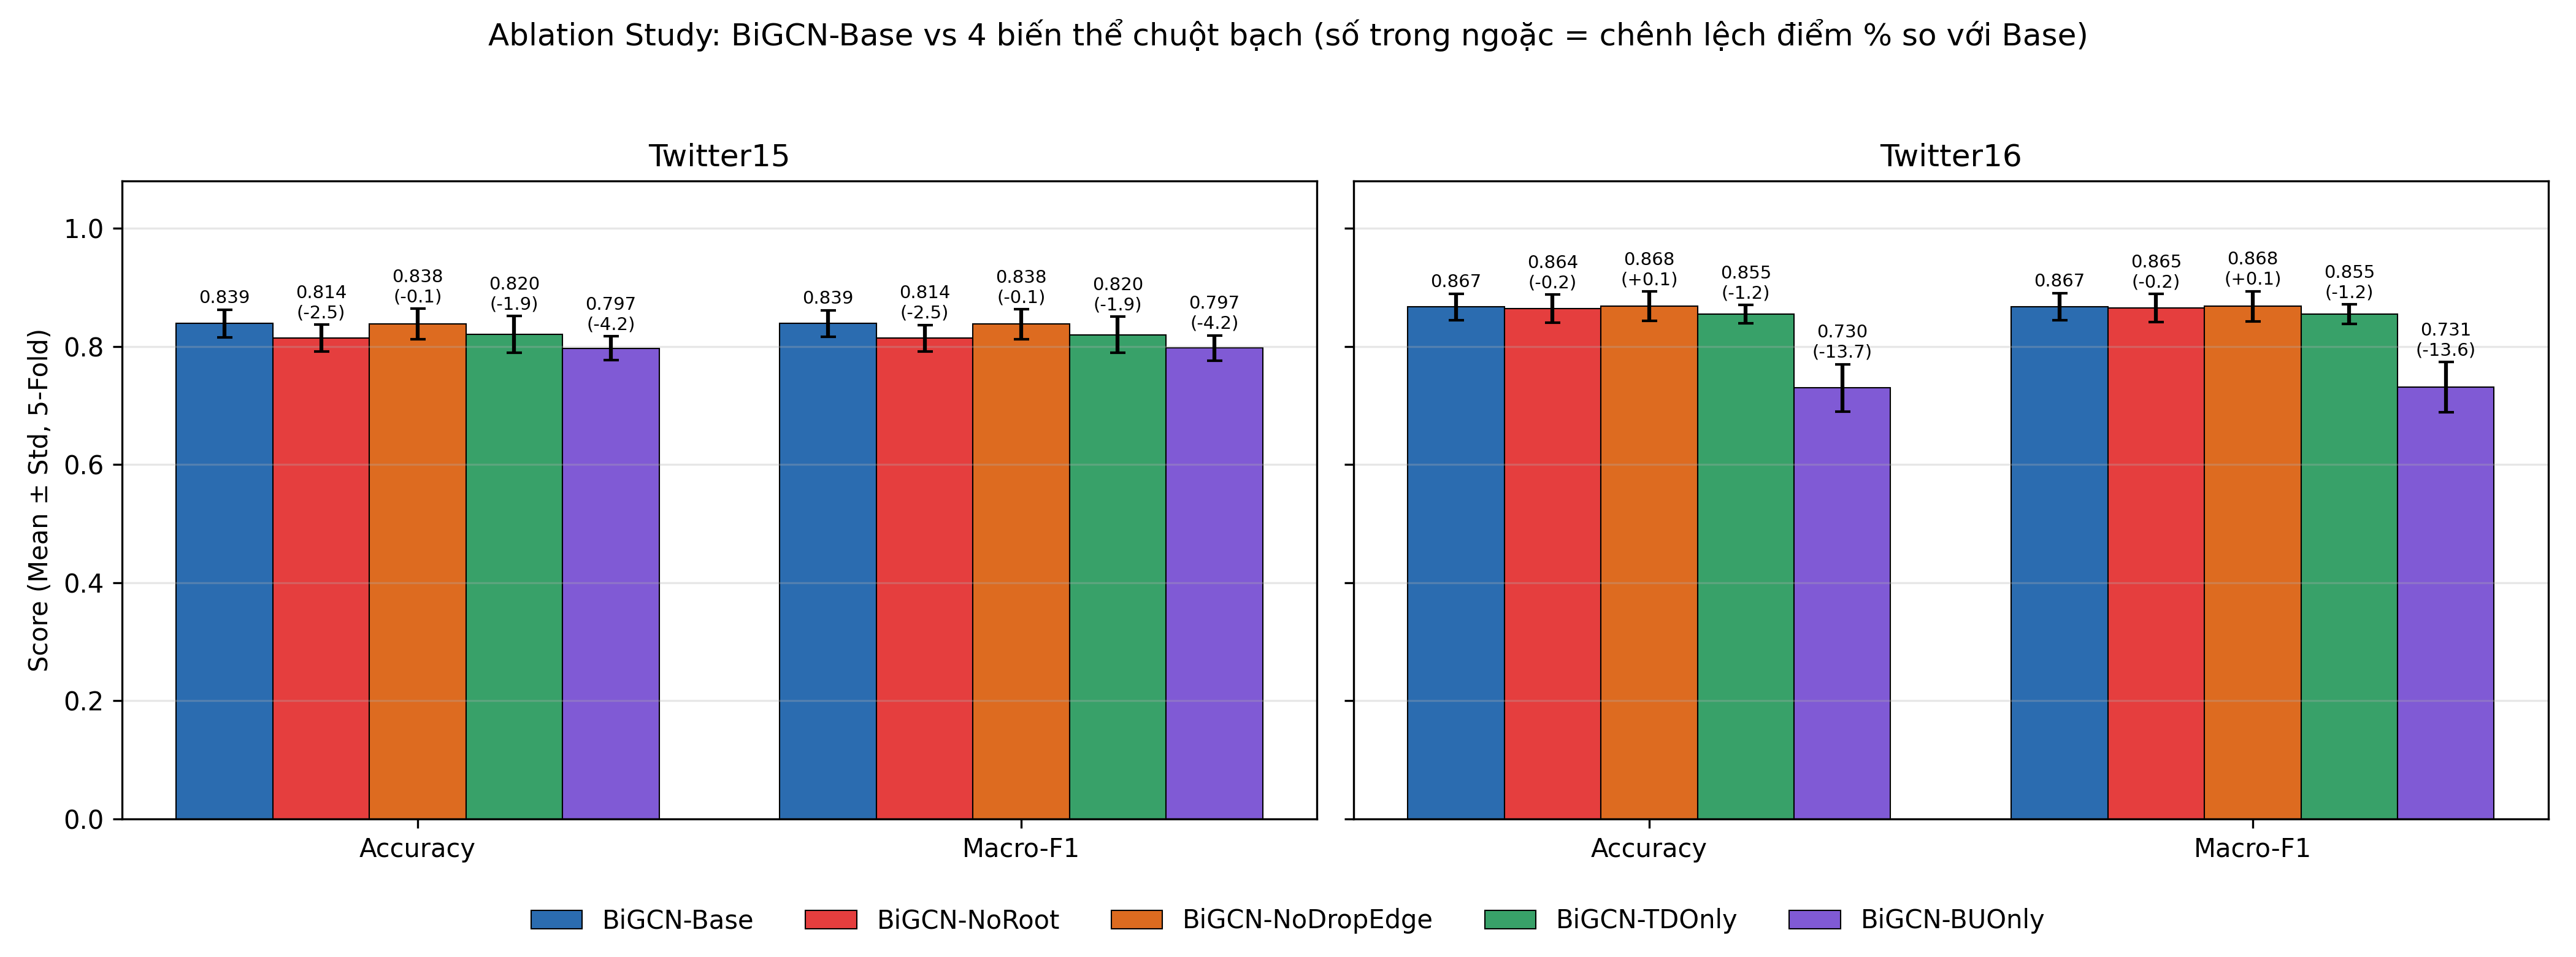
\includegraphics[width=0.94\textwidth]{figures/ablation_comparison.png}
    \caption[So sánh mức suy giảm của 4 biến thể giải phẫu BiGCN]{So sánh trực quan mức độ biến động Accuracy và Macro-F1 của $4$ biến thể giải phẫu so với \texttt{BiGCN-Base} trên Twitter15 và Twitter16 \coderef{scripts/aggregate_results.py}{scripts/aggregate\_results.py}}
    \label{fig:ablation}
\end{figure}

\section{Hiệu năng mô hình đề xuất \texttt{BiGCN-Plus}, Kiểm định thống kê và Đối sánh tổng thể}

Để chứng minh minh bạch đóng góp của từng nhánh kiến trúc cũng như tách biệt ảnh hưởng của mã định danh người dùng, nhóm thực nghiệm đầy đủ $5$ cấu hình Cấp độ 3 gồm \texttt{BiGCN-Plus-B1Only}, \texttt{BiGCN-Plus-B2Only}, \texttt{BiGCN-Plus-B12} (thuần GNN không có Nhánh 3), cấu hình đề xuất chuẩn sạch \textbf{\texttt{BiGCN-Plus-Clean}} (hoàn toàn không dùng User-ID) và biến thể mở rộng \textbf{\texttt{BiGCN-Plus-UserID}} (bổ sung ma trận nhân $K_u$). Toàn bộ kết quả đối sánh $25$ lượt chạy được tổng hợp tại Bảng~\ref{tab:master-comparison}, minh họa tại Hình~\ref{fig:master-chart}, và kiểm định ý nghĩa thống kê ghép cặp tại Bảng~\ref{tab:wilcoxon-tests}:

\begin{itemize}
    \item \textbf{Hiệu năng vượt trội của mô hình chuẩn sạch \texttt{BiGCN-Plus-Clean} (không dùng User-ID):} Trên Twitter15, \texttt{BiGCN-Plus-Clean} đạt độ chính xác trung bình $\mathbf{0{,}85946 \pm 0{,}02188}$ (Macro-F1 $0{,}85946$, MCC $0{,}81344$, AUC-ROC $0{,}97176$), vượt \texttt{BiGCN-Base} ($+0{,}02456$, Wilcoxon $p = 0{,}00006$), vượt \texttt{TF-IDF-Ridge} ($+0{,}02255$, $p = 0{,}00014$) và vượt \texttt{EBGCN} ($+0{,}02792$, $p = 0{,}00002$). Trên Twitter16, \texttt{BiGCN-Plus-Clean} đạt $\mathbf{0{,}87116 \pm 0{,}02724}$ (Macro-F1 $0{,}87145$, AUC-ROC $0{,}97803$), vượt trội có ý nghĩa thống kê so với toàn bộ các baseline Cấp 1--2 và NLP (Wilcoxon $p \le 0{,}00922$).
    \item \textbf{Phân tách đóng góp theo từng nhánh (Branch Ablation):} Trên cả hai bộ dữ liệu, kết hợp song song hai nhánh đồ thị \texttt{BiGCN-Plus-B12} ($0{,}84725$ trên Twitter15; $0{,}86798$ trên Twitter16) đều cải thiện rõ rệt so với từng nhánh đơn lẻ \texttt{B1Only} ($0{,}83866$ / $0{,}81515$) và \texttt{B2Only} ($0{,}84255$ / $0{,}86089$). Khi bổ sung Nhánh 3 sạch (\texttt{Sublinear TF-IDF} + $10$ thống kê đồ thị qua LOO Hat-Matrix), hiệu năng tiếp tục tăng lên $0{,}85946$ và $0{,}87116$.
    \item \textbf{Phân tích tác động của tín hiệu User-ID (\texttt{BiGCN-Plus-UserID}):} Khi bổ sung ma trận nhân tần suất tài khoản $K_u$, \texttt{BiGCN-Plus-UserID} đạt mức đỉnh $\mathbf{0{,}88389 \pm 0{,}01855}$ trên Twitter15 và $\mathbf{0{,}89706 \pm 0{,}02413}$ trên Twitter16 (tăng thêm $+0{,}02443$ và $+0{,}02591$ so với bản sạch, $p < 0{,}0001$). Điều này lượng hóa trung thực rằng khoảng $2{,}5\%$ độ chính xác bổ sung đến từ thông tin mức độ tham gia của các tài khoản quen thuộc trong tập dữ liệu; do đó nhóm đề xuất sử dụng \texttt{BiGCN-Plus-Clean} làm chuẩn đánh giá tổng quát hóa sạch và báo cáo song song \texttt{BiGCN-Plus-UserID} để đối chiếu.
\end{itemize}

\begin{table}[htbp]
    \centering
    \caption[Bảng đối sánh tổng thể 25 lượt các mô hình tiêu biểu qua 3 cấp độ]{Bảng đối sánh tổng thể $25$ lượt chạy ($5\text{ seeds} \times 5\text{ folds}$, GPU T4) của các mô hình tiêu biểu qua 3 cấp độ trên Twitter15 và Twitter16 \coderef{scripts/CT255_RumorDetection_BiGCN_Plus_MultiSeed_5x5_Colab_T4GPU.ipynb}{Colab Cell 3--6}}
    \label{tab:master-comparison}
    \scriptsize
    \setlength{\tabcolsep}{3.2pt}
    \begin{tabular}{@{}lllrrrrrrr@{}}
        \toprule
        \multicolumn{1}{c}{\textbf{Dataset}} & \multicolumn{1}{c}{\textbf{Cấp}} & \multicolumn{1}{c}{\textbf{Mô hình}} & \multicolumn{1}{c}{\textbf{Accuracy}} & \multicolumn{1}{c}{\textbf{Macro-F1}} & \multicolumn{1}{c}{\textbf{F1-NR}} & \multicolumn{1}{c}{\textbf{F1-FR}} & \multicolumn{1}{c}{\textbf{F1-TR}} & \multicolumn{1}{c}{\textbf{F1-UR}} & \multicolumn{1}{c}{\textbf{AUC-ROC}} \\
        \midrule
        Twitter15 & NLP   & \texttt{TF-IDF-Ridge}      & $0{,}83691$ & $0{,}83761$ & $0{,}78400$ & $0{,}83604$ & $0{,}90654$ & $0{,}82387$ & $0{,}95838$ \\
        Twitter15 & Cấp 1 & \texttt{MLP-BoW}           & $0{,}81732$ & $0{,}81735$ & $0{,}75405$ & $0{,}82312$ & $0{,}87879$ & $0{,}81343$ & $0{,}95865$ \\
        Twitter15 & Cấp 1 & \texttt{GCN-Single}        & $0{,}77383$ & $0{,}77417$ & $0{,}79000$ & $0{,}72733$ & $0{,}81399$ & $0{,}76536$ & $0{,}93268$ \\
        Twitter15 & Cấp 1 & \texttt{GAT-Single}        & $0{,}80228$ & $0{,}80296$ & $0{,}77199$ & $0{,}79217$ & $0{,}86665$ & $0{,}78102$ & $0{,}94819$ \\
        Twitter15 & Cấp 1 & \texttt{GraphSAGE-Single}  & $0{,}83020$ & $0{,}83034$ & $0{,}80125$ & $0{,}82496$ & $0{,}87426$ & $0{,}82088$ & $0{,}96105$ \\
        Twitter15 & Cấp 2 & \texttt{BiGCN-Base}        & $0{,}83490$ & $0{,}83509$ & $0{,}84090$ & $0{,}82433$ & $0{,}86917$ & $0{,}80594$ & $0{,}95878$ \\
        Twitter15 & Cấp 2 & \texttt{EBGCN}             & $0{,}83154$ & $0{,}83125$ & $0{,}81348$ & $0{,}82437$ & $0{,}87434$ & $0{,}81280$ & $0{,}96503$ \\
        Twitter15 & Cấp 2 & \texttt{RAGCL}             & $0{,}83007$ & $0{,}83019$ & $0{,}83714$ & $0{,}81575$ & $0{,}86426$ & $0{,}80361$ & $0{,}95541$ \\
        Twitter15 & Cấp 3 & \texttt{BiGCN-Plus-B1Only} & $0{,}83866$ & $0{,}83872$ & $0{,}84903$ & $0{,}82686$ & $0{,}87020$ & $0{,}80879$ & $0{,}95933$ \\
        Twitter15 & Cấp 3 & \texttt{BiGCN-Plus-B2Only} & $0{,}84255$ & $0{,}84253$ & $0{,}82319$ & $0{,}83227$ & $0{,}89005$ & $0{,}82461$ & $0{,}96779$ \\
        Twitter15 & Cấp 3 & \texttt{BiGCN-Plus-B12}    & $0{,}84725$ & $0{,}84718$ & $0{,}83412$ & $0{,}83723$ & $0{,}88771$ & $0{,}82967$ & $0{,}96846$ \\
        Twitter15 & Cấp 3 & \textit{\texttt{BiGCN-Plus-Clean}}  & $\mathit{0{,}85946}$ & $\mathit{0{,}85946}$ & $\mathit{0{,}85021}$ & $\mathit{0{,}84656}$ & $\mathit{0{,}89984}$ & $\mathit{0{,}84126}$ & $\mathit{0{,}97176}$ \\
        Twitter15 & Cấp 3 & \textbf{\texttt{BiGCN-Plus-UserID}} & $\mathbf{0{,}88389}$ & $\mathbf{0{,}88371}$ & $\mathbf{0{,}89464}$ & $\mathbf{0{,}86903}$ & $\mathbf{0{,}91476}$ & $\mathbf{0{,}85639}$ & $\mathbf{0{,}98109}$ \\
        \addlinespace[4pt]
        Twitter16 & NLP   & \texttt{TF-IDF-Ridge}      & $0{,}85230$ & $0{,}85304$ & $0{,}77696$ & $0{,}83705$ & $0{,}91674$ & $0{,}88140$ & $0{,}96446$ \\
        Twitter16 & Cấp 1 & \texttt{MLP-BoW}           & $0{,}84450$ & $0{,}84437$ & $0{,}75354$ & $0{,}84001$ & $0{,}89982$ & $0{,}88412$ & $0{,}96907$ \\
        Twitter16 & Cấp 1 & \texttt{GCN-Single}        & $0{,}65356$ & $0{,}64670$ & $0{,}69970$ & $0{,}47822$ & $0{,}82281$ & $0{,}58605$ & $0{,}87422$ \\
        Twitter16 & Cấp 1 & \texttt{GAT-Single}        & $0{,}84206$ & $0{,}84347$ & $0{,}78679$ & $0{,}82170$ & $0{,}89048$ & $0{,}87493$ & $0{,}96440$ \\
        Twitter16 & Cấp 1 & \texttt{GraphSAGE-Single}  & $0{,}86137$ & $0{,}86122$ & $0{,}82015$ & $0{,}83911$ & $0{,}89906$ & $0{,}88657$ & $0{,}97170$ \\
        Twitter16 & Cấp 2 & \texttt{BiGCN-Base}        & $0{,}81345$ & $0{,}81428$ & $0{,}77299$ & $0{,}77351$ & $0{,}86824$ & $0{,}84237$ & $0{,}95426$ \\
        Twitter16 & Cấp 2 & \texttt{EBGCN}             & $0{,}85478$ & $0{,}85479$ & $0{,}82644$ & $0{,}83108$ & $0{,}89517$ & $0{,}86648$ & $0{,}97251$ \\
        Twitter16 & Cấp 2 & \texttt{RAGCL}             & $0{,}79977$ & $0{,}80103$ & $0{,}75758$ & $0{,}76306$ & $0{,}85412$ & $0{,}82936$ & $0{,}94619$ \\
        Twitter16 & Cấp 3 & \texttt{BiGCN-Plus-B1Only} & $0{,}81515$ & $0{,}81587$ & $0{,}77837$ & $0{,}78190$ & $0{,}86691$ & $0{,}83631$ & $0{,}95594$ \\
        Twitter16 & Cấp 3 & \texttt{BiGCN-Plus-B2Only} & $0{,}86089$ & $0{,}86118$ & $0{,}80799$ & $0{,}84061$ & $0{,}90892$ & $0{,}88719$ & $0{,}97386$ \\
        Twitter16 & Cấp 3 & \texttt{BiGCN-Plus-B12}    & $0{,}86798$ & $0{,}86841$ & $0{,}83065$ & $0{,}84693$ & $0{,}90729$ & $0{,}88876$ & $0{,}97516$ \\
        Twitter16 & Cấp 3 & \textit{\texttt{BiGCN-Plus-Clean}}  & $\mathit{0{,}87116}$ & $\mathit{0{,}87145}$ & $\mathit{0{,}83204}$ & $\mathit{0{,}85292}$ & $\mathit{0{,}90801}$ & $\mathit{0{,}89283}$ & $\mathit{0{,}97803}$ \\
        Twitter16 & Cấp 3 & \textbf{\texttt{BiGCN-Plus-UserID}} & $\mathbf{0{,}89706}$ & $\mathbf{0{,}89702}$ & $\mathbf{0{,}88173}$ & $\mathbf{0{,}87060}$ & $\mathbf{0{,}92165}$ & $\mathbf{0{,}91411}$ & $\mathbf{0{,}98611}$ \\
        \bottomrule
    \end{tabular}
    \par\vspace{3pt}
    {\footnotesize\textit{Ghi chú: Giá trị \textbf{in đậm} biểu thị kết quả cao nhất toàn bảng (có $K_u$); giá trị \textit{in nghiêng} biểu thị kết quả cao nhất trong nhóm mô hình chuẩn sạch không dùng User-ID.}}
\end{table}

\begin{table}[htbp]
    \centering
    \caption[Kiểm định thống kê Paired t-test và Wilcoxon đối với BiGCN-Plus-Clean]{Kết quả kiểm định ý nghĩa thống kê ghép cặp (\textit{Paired t-test} và \textit{Wilcoxon signed-rank}, $N = 25$ cặp) giữa các mô hình đối sánh với \texttt{BiGCN-Plus-Clean} \coderef{results/tables/statistical_tests.md}{statistical\_tests.md}}
    \label{tab:wilcoxon-tests}
    \footnotesize
    \setlength{\tabcolsep}{4.5pt}
    \begin{tabular}{@{}llrrrr@{}}
        \toprule
        \multicolumn{1}{c}{\textbf{Dataset}} & \multicolumn{1}{c}{\textbf{Mô hình so sánh ($A$) vs \texttt{BiGCN-Plus-Clean} ($B$)}} & \multicolumn{1}{c}{\textbf{$\Delta\text{Acc}\;(A-B)$}} & \multicolumn{1}{c}{\textbf{$p$-value (Paired-$t$)}} & \multicolumn{1}{c}{\textbf{$p$-value (Wilcoxon)}} & \multicolumn{1}{c}{\textbf{Ý nghĩa ($\alpha = 0{,}05$)}} \\
        \midrule
        Twitter15 & \texttt{TF-IDF-Ridge}      & $-0{,}02255$ & $0{,}00001$ & $0{,}00014$ & Có ($p < 0{,}001$) \\
        Twitter15 & \texttt{MLP-BoW}           & $-0{,}04215$ & $< 0{,}00001$ & $0{,}00001$ & Có ($p < 0{,}001$) \\
        Twitter15 & \texttt{GraphSAGE-Single}  & $-0{,}02926$ & $< 0{,}00001$ & $0{,}00001$ & Có ($p < 0{,}001$) \\
        Twitter15 & \texttt{BiGCN-Base}        & $-0{,}02456$ & $< 0{,}00001$ & $0{,}00006$ & Có ($p < 0{,}001$) \\
        Twitter15 & \texttt{EBGCN}             & $-0{,}02792$ & $< 0{,}00001$ & $0{,}00002$ & Có ($p < 0{,}001$) \\
        Twitter15 & \texttt{RAGCL}             & $-0{,}02940$ & $< 0{,}00001$ & $0{,}00006$ & Có ($p < 0{,}001$) \\
        Twitter15 & \texttt{BiGCN-Plus-B12}    & $-0{,}01221$ & $< 0{,}00001$ & $0{,}00003$ & Có ($p < 0{,}001$) \\
        Twitter15 & \texttt{BiGCN-Plus-UserID} & $+0{,}02443$ & $< 0{,}00001$ & $0{,}00001$ & Có ($p < 0{,}001$) \\
        \addlinespace[4pt]
        Twitter16 & \texttt{TF-IDF-Ridge}      & $-0{,}01886$ & $0{,}00168$ & $0{,}00411$ & Có ($p < 0{,}01$) \\
        Twitter16 & \texttt{MLP-BoW}           & $-0{,}02666$ & $< 0{,}00001$ & $0{,}00004$ & Có ($p < 0{,}001$) \\
        Twitter16 & \texttt{GraphSAGE-Single}  & $-0{,}00979$ & $0{,}00891$ & $0{,}00922$ & Có ($p < 0{,}01$) \\
        Twitter16 & \texttt{BiGCN-Base}        & $-0{,}05771$ & $< 0{,}00001$ & $0{,}00001$ & Có ($p < 0{,}001$) \\
        Twitter16 & \texttt{EBGCN}             & $-0{,}01638$ & $0{,}00011$ & $0{,}00106$ & Có ($p < 0{,}01$) \\
        Twitter16 & \texttt{RAGCL}             & $-0{,}07139$ & $< 0{,}00001$ & $0{,}00001$ & Có ($p < 0{,}001$) \\
        Twitter16 & \texttt{BiGCN-Plus-B12}    & $-0{,}00318$ & $0{,}12511$ & $0{,}08371$ & Không ($p > 0{,}05$) \\
        Twitter16 & \texttt{BiGCN-Plus-UserID} & $+0{,}02591$ & $< 0{,}00001$ & $0{,}00007$ & Có ($p < 0{,}001$) \\
        \bottomrule
    \end{tabular}
    \par\vspace{3pt}
    {\footnotesize\textit{Ghi chú: Giá trị âm $\Delta\text{Acc} < 0$ cho thấy \texttt{BiGCN-Plus-Clean} vượt trội mô hình đối sánh; kiểm định thực hiện trên đúng $25$ cặp $(seed, fold)$ đồng nhất.}}
\end{table}

\begin{figure}[htbp]
    \centering
    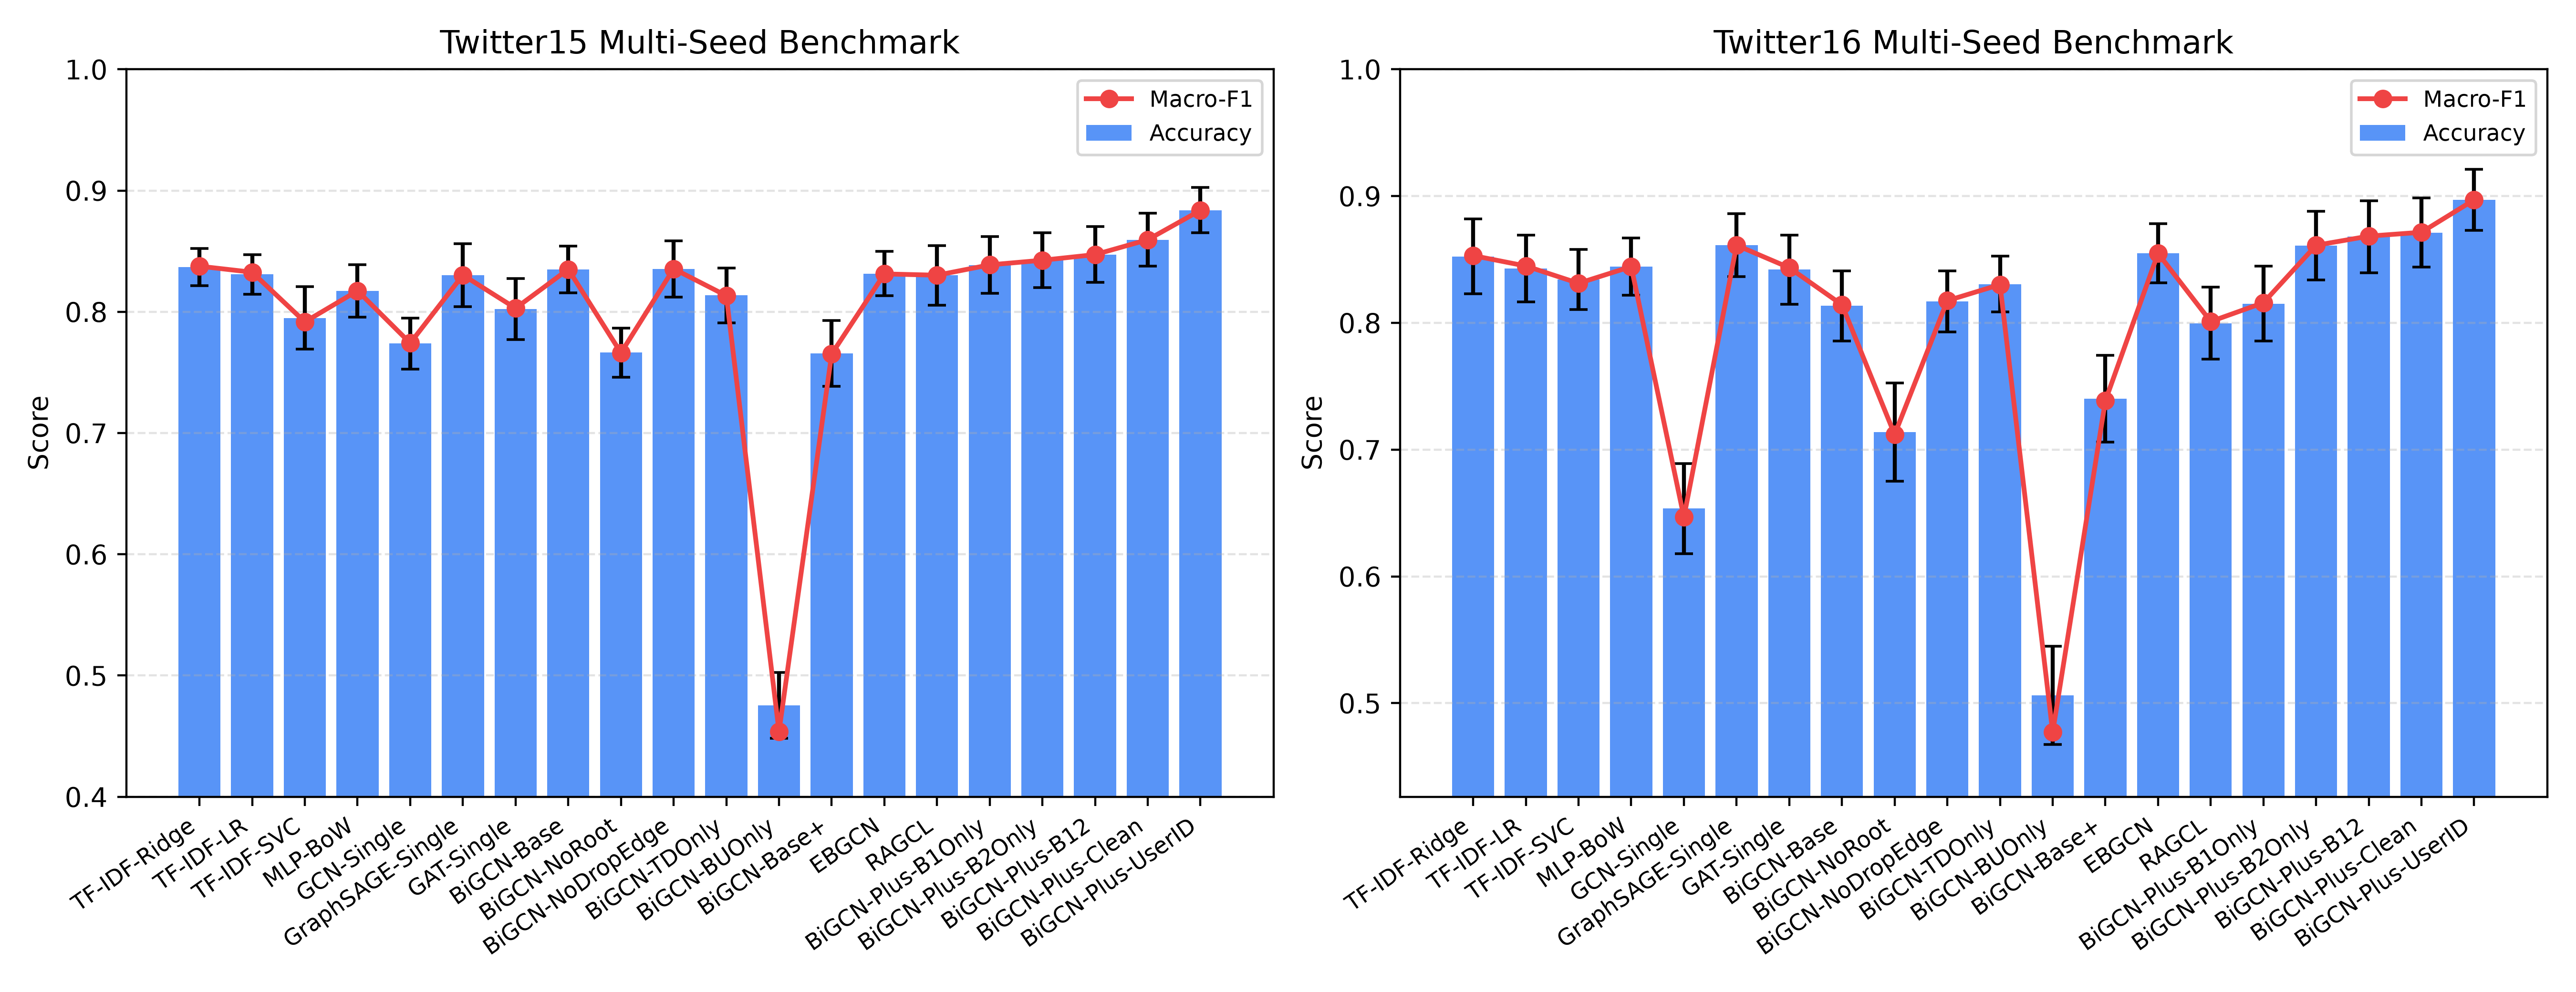
\includegraphics[width=0.96\textwidth]{figures/multiseed_comparison.png}
    \caption[Biểu đồ đối sánh Accuracy và Macro-F1 qua 20 mô hình (25 lượt chạy)]{Biểu đồ đối sánh Accuracy (kèm thanh sai số độ lệch chuẩn) và Macro-F1 của $20$ mô hình thực nghiệm qua $25$ lượt chạy trên Twitter15 và Twitter16 \coderef{scripts/aggregate_results.py}{scripts/aggregate\_results.py}}
    \label{fig:master-chart}
\end{figure}

Đường cong hội tụ huấn luyện và ma trận nhầm lẫn cộng dồn của cấu hình chuẩn sạch \texttt{BiGCN-Plus-Clean} được trình bày chi tiết dưới dạng hình phức hợp tại Hình~\ref{fig:bigcn-plus-curves} và Hình~\ref{fig:bigcn-plus-cm}. Quan sát Hình~\ref{fig:bigcn-plus-curves}(a) và Hình~\ref{fig:bigcn-plus-curves}(b) cho thấy hàm mất mát huấn luyện giảm đều và hiệu năng kiểm thử đạt trạng thái ổn định vững chắc từ epoch $60$ đến epoch $100$ mà không xuất hiện hiện tượng phân kỳ quá khớp trên cả hai tập dữ liệu. Phân tích ma trận nhầm lẫn tại Hình~\ref{fig:bigcn-plus-cm}(a) và Hình~\ref{fig:bigcn-plus-cm}(b) cho thấy mô hình phân tách rất tốt lớp \textit{True Rumor} ($F_1\text{-TR}$ đạt $0{,}89984$ trên Twitter15 và $0{,}90801$ trên Twitter16), trong khi phần lớn lỗi tập trung ở sự giao thoa văn phong giữa lớp \textit{False Rumor} và \textit{Non-Rumor} do dữ liệu mở chưa có văn bản bình luận phản bác từ cộng đồng.

\begin{figure}[htbp]
    \centering
    \begin{subfigure}[b]{0.48\textwidth}
        \centering
        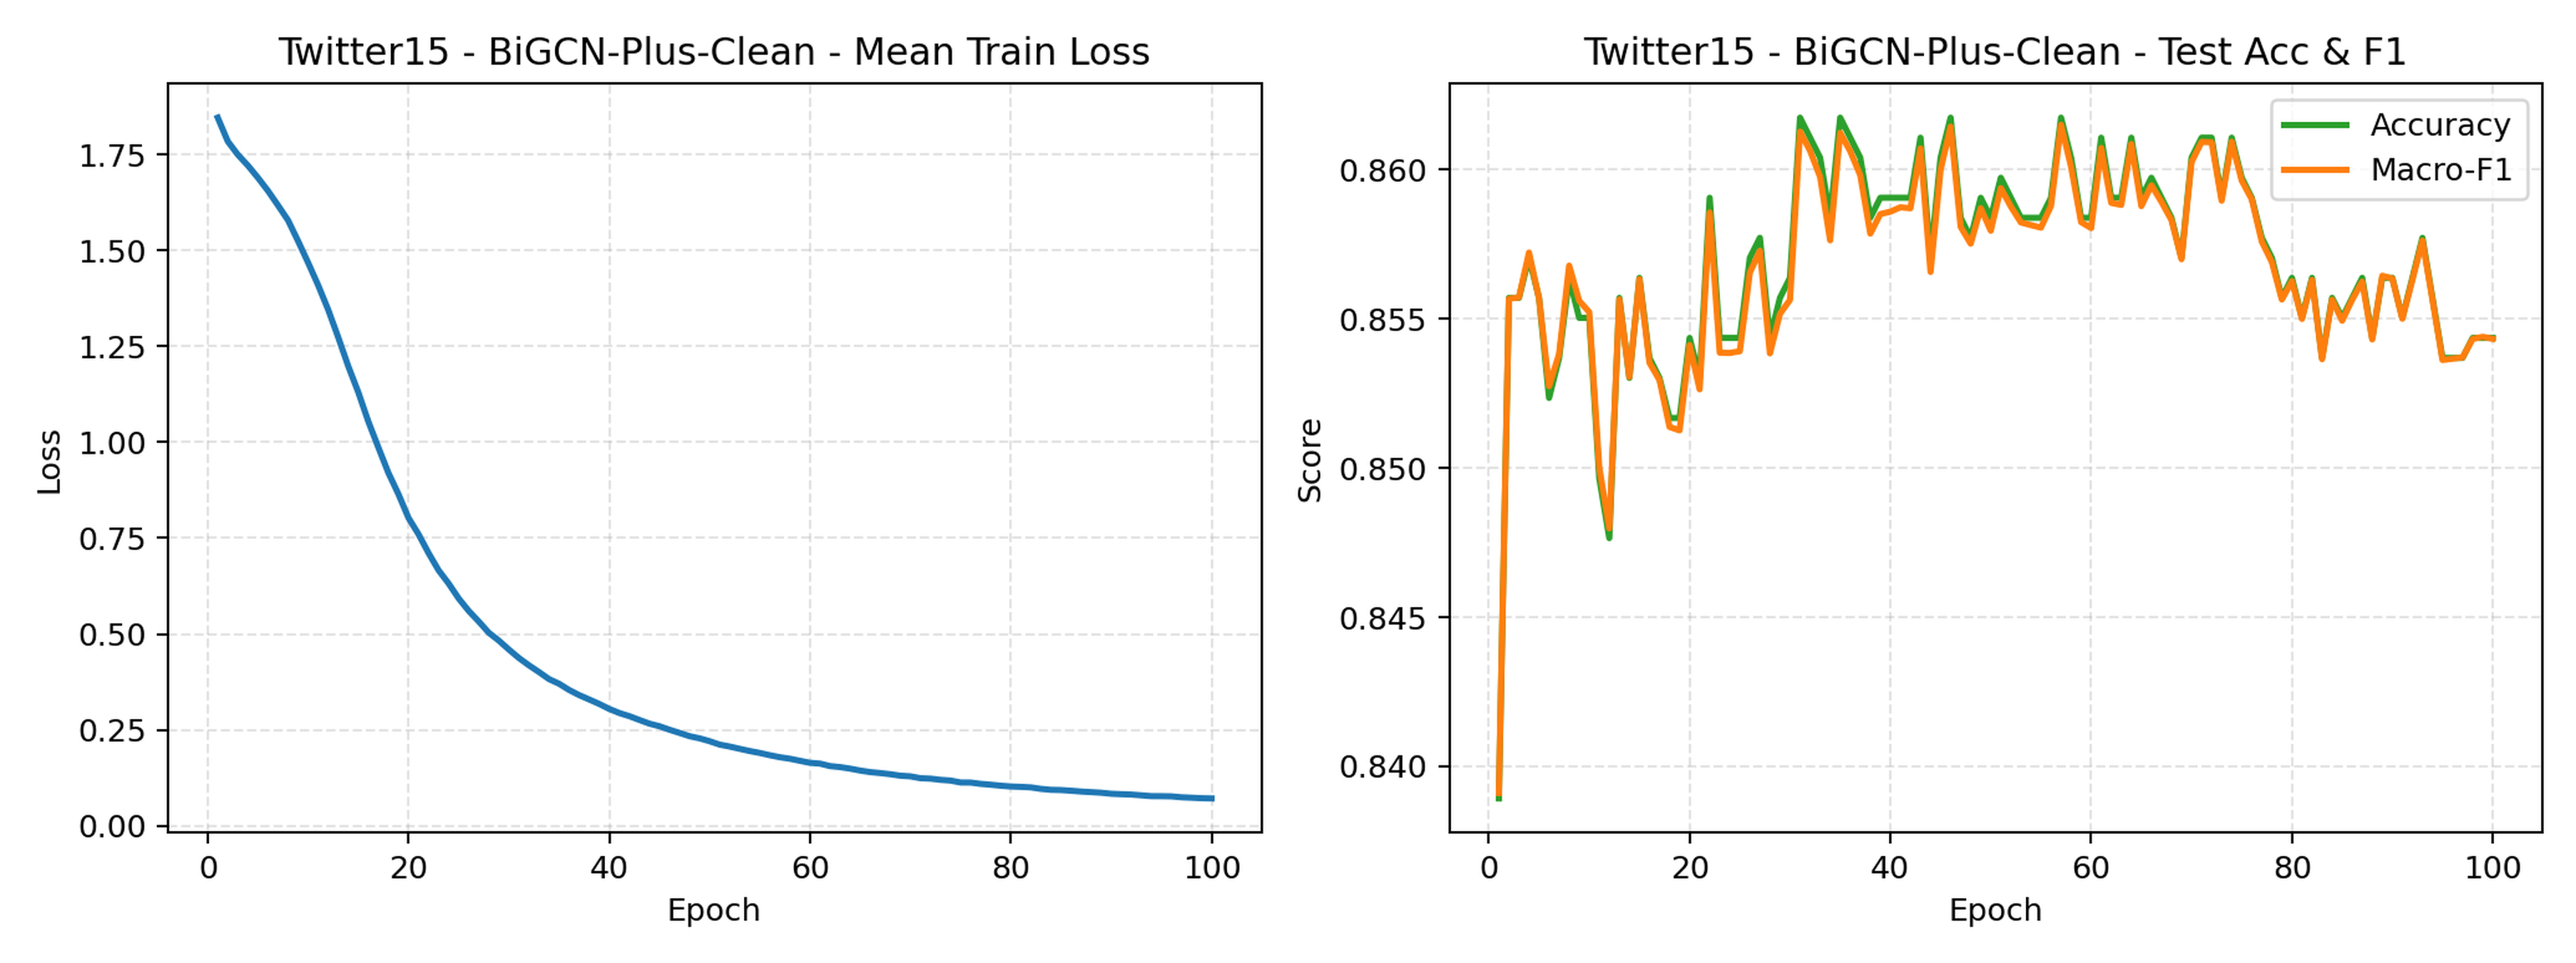
\includegraphics[width=\textwidth]{figures/bigcn_plus_clean_t15_curves.png}
        \caption{Đường cong huấn luyện trên Twitter15}
        \label{fig:bigcn-plus-curves-t15}
    \end{subfigure}
    \hfill
    \begin{subfigure}[b]{0.48\textwidth}
        \centering
        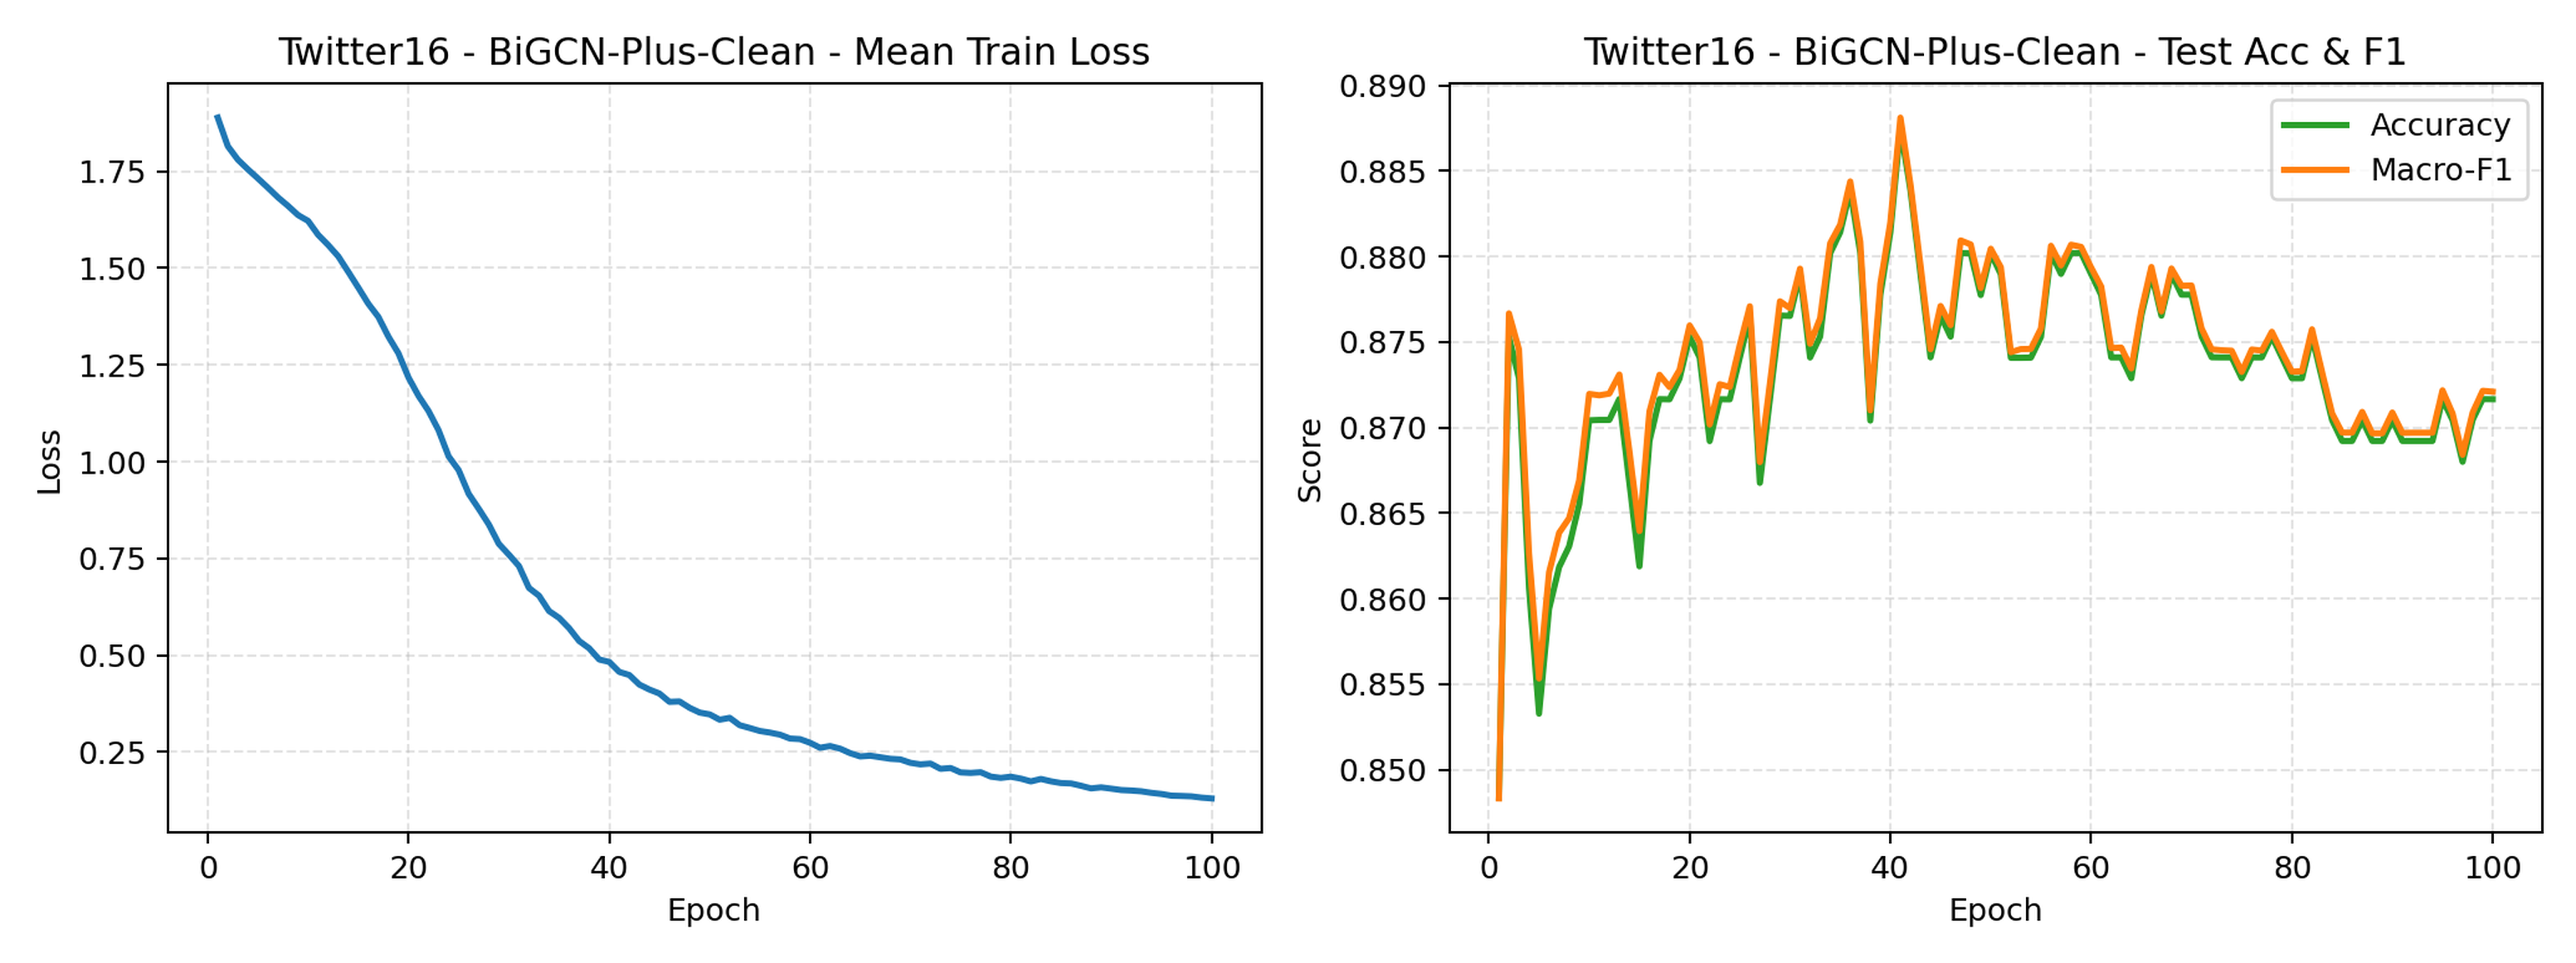
\includegraphics[width=\textwidth]{figures/bigcn_plus_clean_t16_curves.png}
        \caption{Đường cong huấn luyện trên Twitter16}
        \label{fig:bigcn-plus-curves-t16}
    \end{subfigure}
    \caption[Đường cong Loss và Accuracy của BiGCN-Plus-Clean]{Đường cong Loss, Accuracy và Macro-F1 qua $100$ epoch của \texttt{BiGCN-Plus-Clean}: (a) tập dữ liệu Twitter15; (b) tập dữ liệu Twitter16 \coderef{scripts/CT255_RumorDetection_BiGCN_Plus_MultiSeed_5x5_Colab_T4GPU.ipynb}{Colab Cell 5}}
    \label{fig:bigcn-plus-curves}
\end{figure}

\begin{figure}[htbp]
    \centering
    \begin{subfigure}[b]{0.47\textwidth}
        \centering
        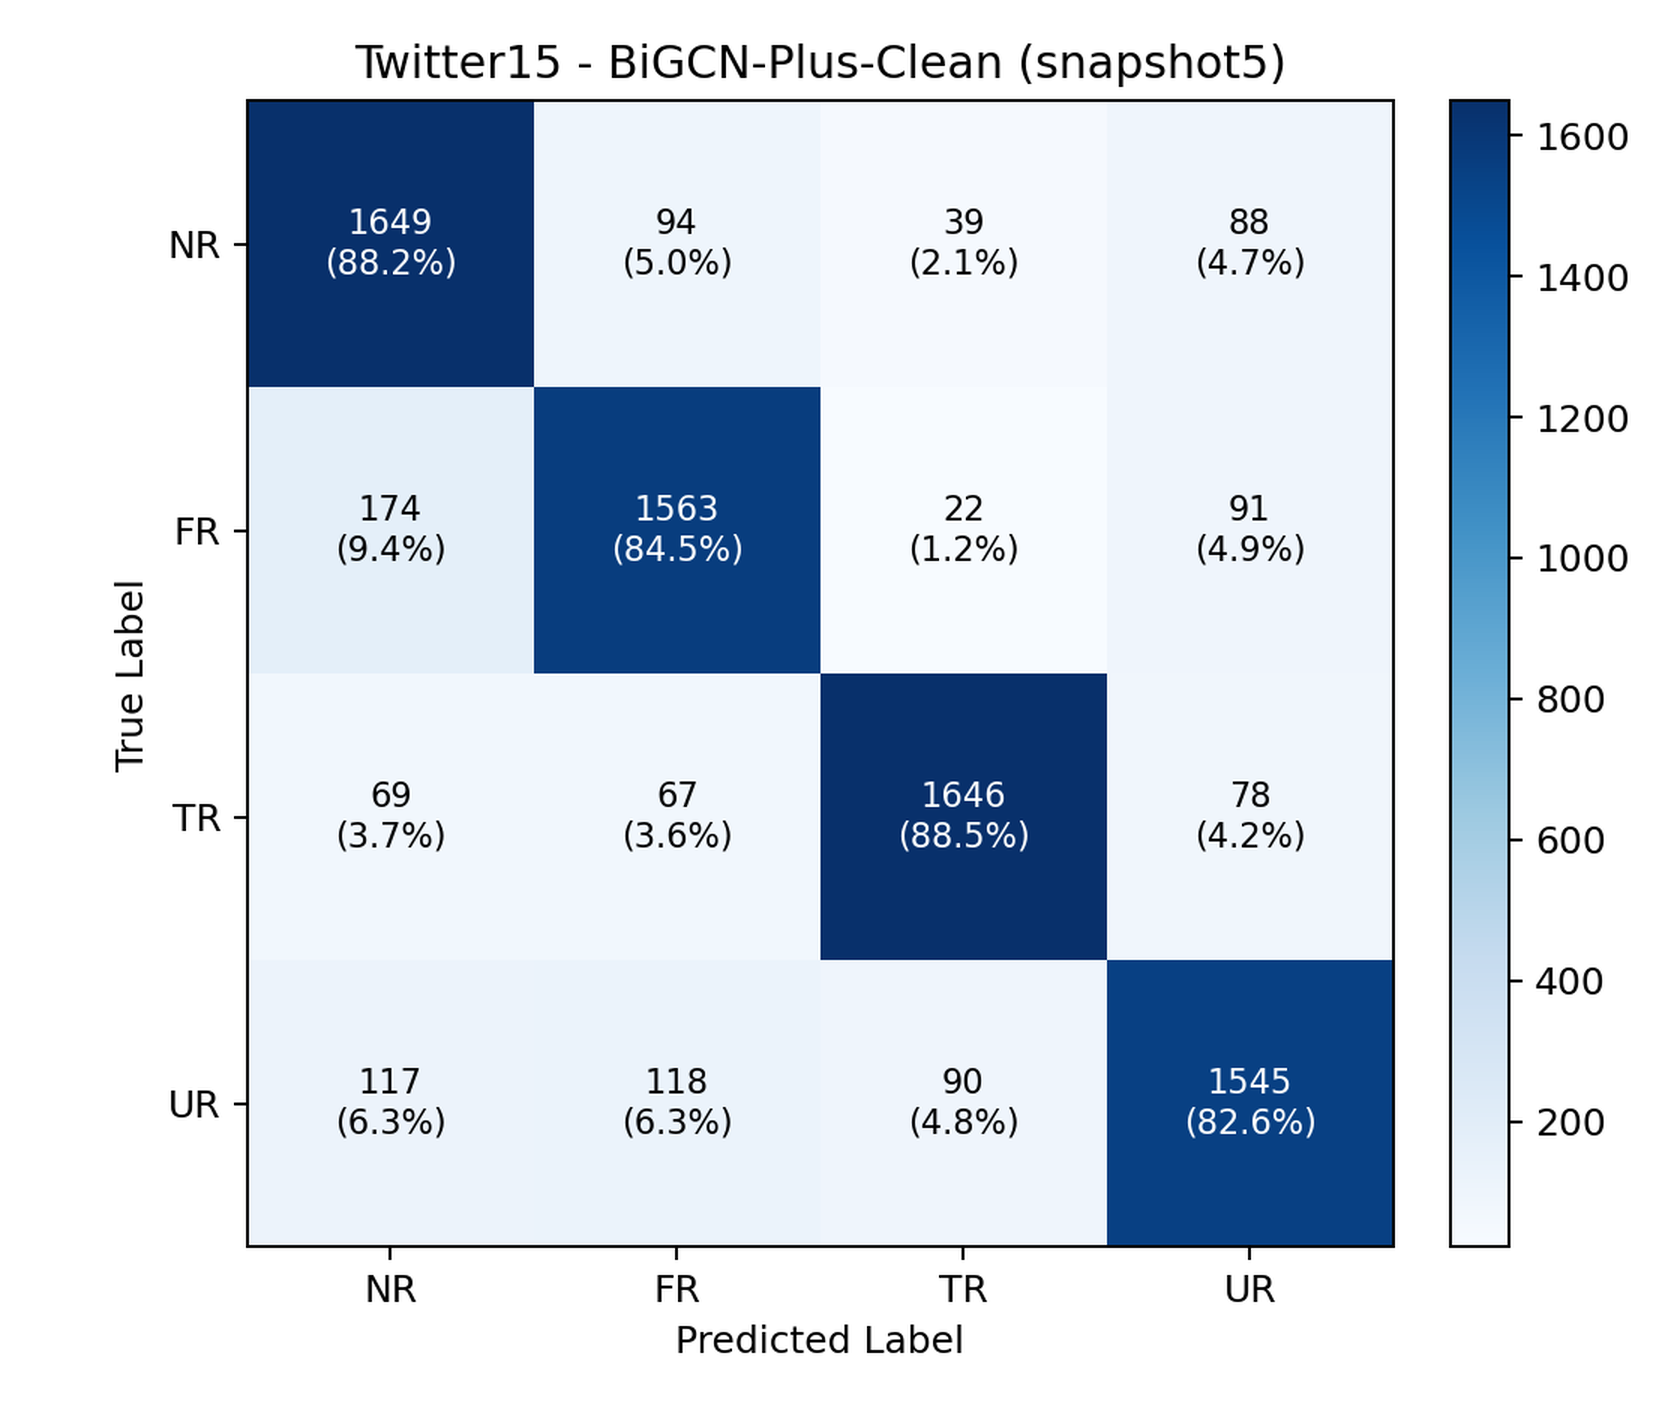
\includegraphics[width=\textwidth]{figures/bigcn_plus_clean_t15_cm.png}
        \caption{Ma trận nhầm lẫn trên Twitter15}
        \label{fig:bigcn-plus-cm-t15}
    \end{subfigure}
    \hfill
    \begin{subfigure}[b]{0.47\textwidth}
        \centering
        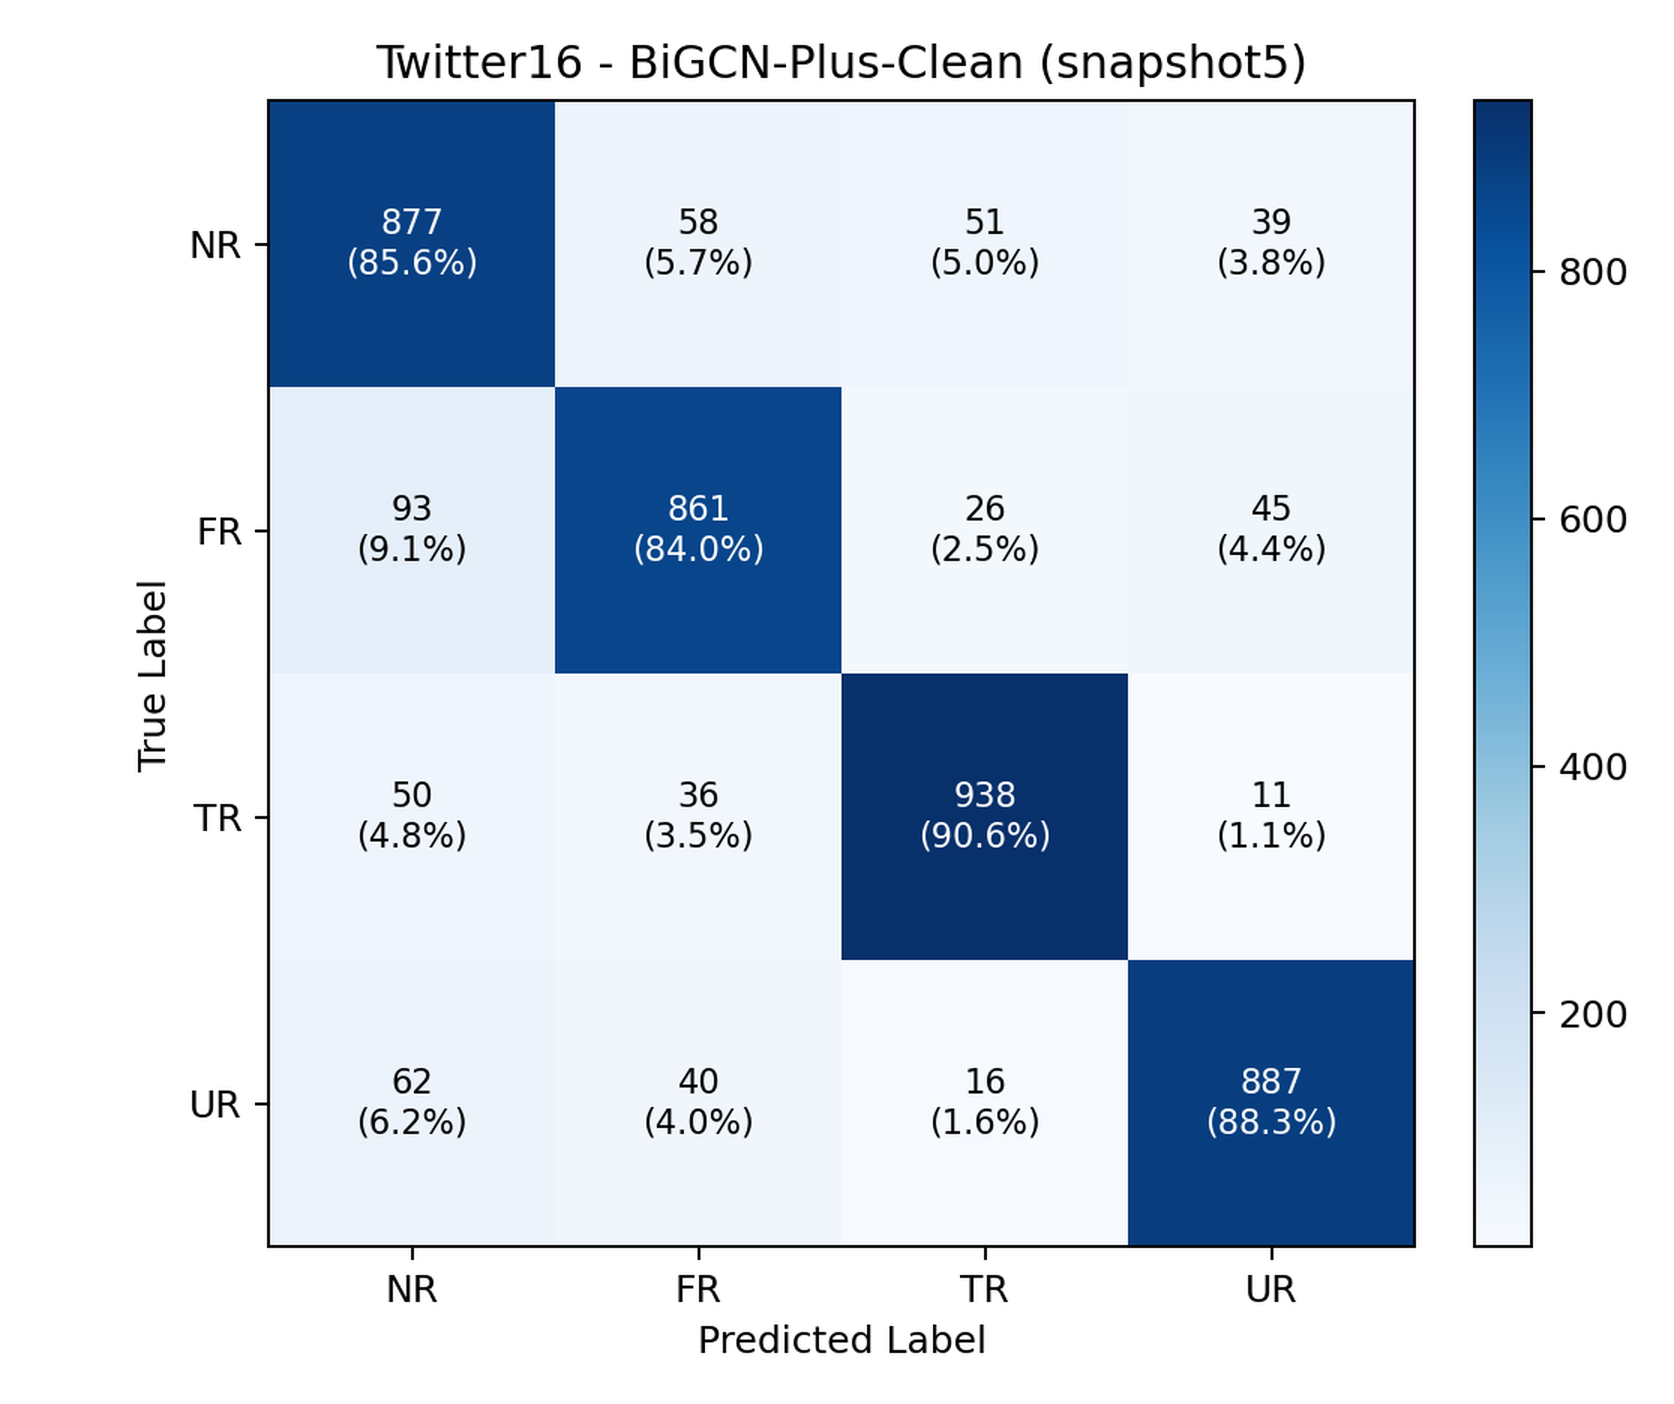
\includegraphics[width=\textwidth]{figures/bigcn_plus_clean_t16_cm.png}
        \caption{Ma trận nhầm lẫn trên Twitter16}
        \label{fig:bigcn-plus-cm-t16}
    \end{subfigure}
    \caption[Ma trận nhầm lẫn cộng dồn 25 lượt của BiGCN-Plus-Clean]{Ma trận nhầm lẫn cộng dồn qua $25$ lượt chạy ($5\text{ seeds} \times 5\text{ folds}$) của \texttt{BiGCN-Plus-Clean}: (a) tập dữ liệu Twitter15; (b) tập dữ liệu Twitter16 \coderef{scripts/CT255_RumorDetection_BiGCN_Plus_MultiSeed_5x5_Colab_T4GPU.ipynb}{Colab Cell 5}}
    \label{fig:bigcn-plus-cm}
\end{figure}

\section{Định vị kết quả so với các công trình công bố trên Twitter15 và Twitter16}

Khi đối chiếu hiệu năng của mô hình đề xuất với các công trình quốc tế đã công bố trên cùng hai bộ chuẩn Twitter15 ($1.490$ cây) và Twitter16 ($818$ cây), cần phân biệt rạch ròi hai chế độ dữ liệu đầu vào: \textbf{Nhóm A} (tập mở \texttt{rumdetect2017} không chứa văn bản bình luận phản hồi, cùng điều kiện với nhóm) và \textbf{Nhóm B} (sử dụng đầy đủ văn bản bình luận thu thập qua API cũ, kết hợp BERT/RoBERTa hoặc đồ thị người dùng/tri thức ngoài). Vị trí định vị tổng thể được tổng hợp tại Bảng~\ref{tab:external-sota} và trực quan hóa trên mặt phẳng hai chiều tại Hình~\ref{fig:external-positioning}.

\begin{table}[htbp]
    \centering
    \caption[Định vị hiệu năng với các công trình công bố trên Twitter15 và Twitter16]{Định vị hiệu năng (Accuracy) của mô hình đề xuất so với các công trình công bố trên Twitter15 và Twitter16 theo điều kiện dữ liệu đầu vào \coderef{results/tables/external_benchmark_sota.md}{external\_benchmark\_sota.md}}
    \label{tab:external-sota}
    \scriptsize
    \setlength{\tabcolsep}{4pt}
    \begin{tabular}{@{}llrrl@{}}
        \toprule
        \multicolumn{1}{c}{\textbf{Điều kiện dữ liệu}} & \multicolumn{1}{c}{\textbf{Phương pháp \& Công bố}} & \multicolumn{1}{c}{\textbf{Twitter15 Acc}} & \multicolumn{1}{c}{\textbf{Twitter16 Acc}} & \multicolumn{1}{c}{\textbf{Giao thức}} \\
        \midrule
        \multicolumn{5}{l}{\textit{Nhóm B -- Có đầy đủ văn bản bình luận phản hồi $\pm$ BERT / Tri thức / Mạng Follow}} \\
        Đồ thị dị thể Tweet--Word--User + VGAE & MLI-GRA (Sci. Rep. 2025) & $0{,}92000$ & $0{,}92900$ & 70/15/15 split \\
        BERT trên mọi node + Graph Autoencoder & GARD (WWW 2024) \cite{tao_semantic_2024} & $0{,}91100$ & $0{,}93200$ & 5-Fold CV \\
        GloVe + Mạng Follow/Reply người dùng & PESTO (WASSA 2023) \cite{noauthor_pesto_2023} & $0{,}91500$ & $0{,}90800$ & 5-Fold CV \\
        BERT trên mọi tweet + BiGCN & ICP-BGCN (Appl. Sci. 2025) \cite{noauthor_integrating_2025} & $0{,}89700$ & $0{,}91700$ & 5-Fold CV \\
        Full text + Transformer-GCN & TRGCN (Nature HSSC 2026) \cite{yan_trgcn_2026} & $0{,}89400$ & $0{,}90100$ & Early stop Val \\
        Full text + Bayesian Edge Uncertainty & EBGCN (ACL 2021) \cite{wei_towards_2021} & $0{,}89200$ & $0{,}91500$ & 5-Fold CV \\
        Wikidata/Probase + Attention-GCN & KAGN (J. Big Data 2023) \cite{noauthor_kagn_2023} & $0{,}89230$ & $0{,}90130$ & 5-Fold CV \\
        RL Key Graph + BERT ghép bình luận & KPG (WWW 2025) & $0{,}89300$ & $0{,}88900$ & 5-Fold CV \\
        Tree Transformer + Pretrain & P2T3 (2026) \cite{cui_avoiding_2026} & $0{,}87400$ & $0{,}91100$ & 10 random splits \\
        Full replies + RoBERTa + InfoNCE & RAGCL (AAAI 2024) \cite{cui_propagation_2024} & $0{,}86700$ & $0{,}90500$ & 10 random splits \\
        Full replies TF-IDF + BiGCN gốc & Bi-GCN (AAAI 2020) & $0{,}88600$ & $0{,}88000$ & 5-Fold CV \\
        Global Struct + Publisher Credibility & GS-PC (2025) & $0{,}84700$ & $0{,}88600$ & 30 runs + Wilcoxon \\
        \addlinespace[4pt]
        \multicolumn{5}{l}{\textit{Nhóm A -- Tập mở \texttt{rumdetect2017} (chỉ có text bài gốc, KHÔNG có text phản hồi)}} \\
        Source-only (tái lập trong RAGCL 2024) & BiGCN Re-impl (AAAI 2024) \cite{cui_propagation_2024} & $0{,}84400$ & $0{,}88000$ & 10 random splits \\
        Source-only (tái lập trong BiTGN 2023) & BiGCN Re-impl (EMNLP 2023) & $0{,}84020$ & $0{,}87330$ & 5-Fold CV \\
        Source TF-IDF (Cui \& Jia, COLING 2025) & BiGCN (TF-IDF) \cite{noauthor_enhancing_2025} & $0{,}81800$ & $0{,}84700$ & 5-Fold / Multi-split \\
        Source Word/Char TF-IDF (nhóm, 25 lượt) & \texttt{TF-IDF-Ridge} & $0{,}83691$ & $0{,}85230$ & $5\text{ seeds} \times 5\text{ folds}$ \\
        Source TF-IDF + BiGCN + DualSAGE (sạch) & \textit{\texttt{BiGCN-Plus-Clean} (nhóm, 25 lượt)} & $\mathit{0{,}85946}$ & $\mathit{0{,}87116}$ & $5\text{ seeds} \times 5\text{ folds}$ \\
        Source TF-IDF + BiGCN + DualSAGE + $K_u$ & \textbf{\texttt{BiGCN-Plus-UserID} (nhóm, 25 lượt)} & $\mathbf{0{,}88389}$ & $\mathbf{0{,}89706}$ & $5\text{ seeds} \times 5\text{ folds}$ \\
        \bottomrule
    \end{tabular}
    \par\vspace{3pt}
    {\footnotesize\textit{Ghi chú: Các số liệu của công trình tham khảo được quy đổi đồng nhất về thang $[0, 1]$ với $5$ chữ số thập phân; giá trị \textbf{in đậm} và \textit{in nghiêng} lần lượt biểu thị hai biến thể đề xuất của nhóm đạt kết quả dẫn đầu trong Nhóm A.}}
\end{table}

\begin{figure}[htbp]
    \centering
    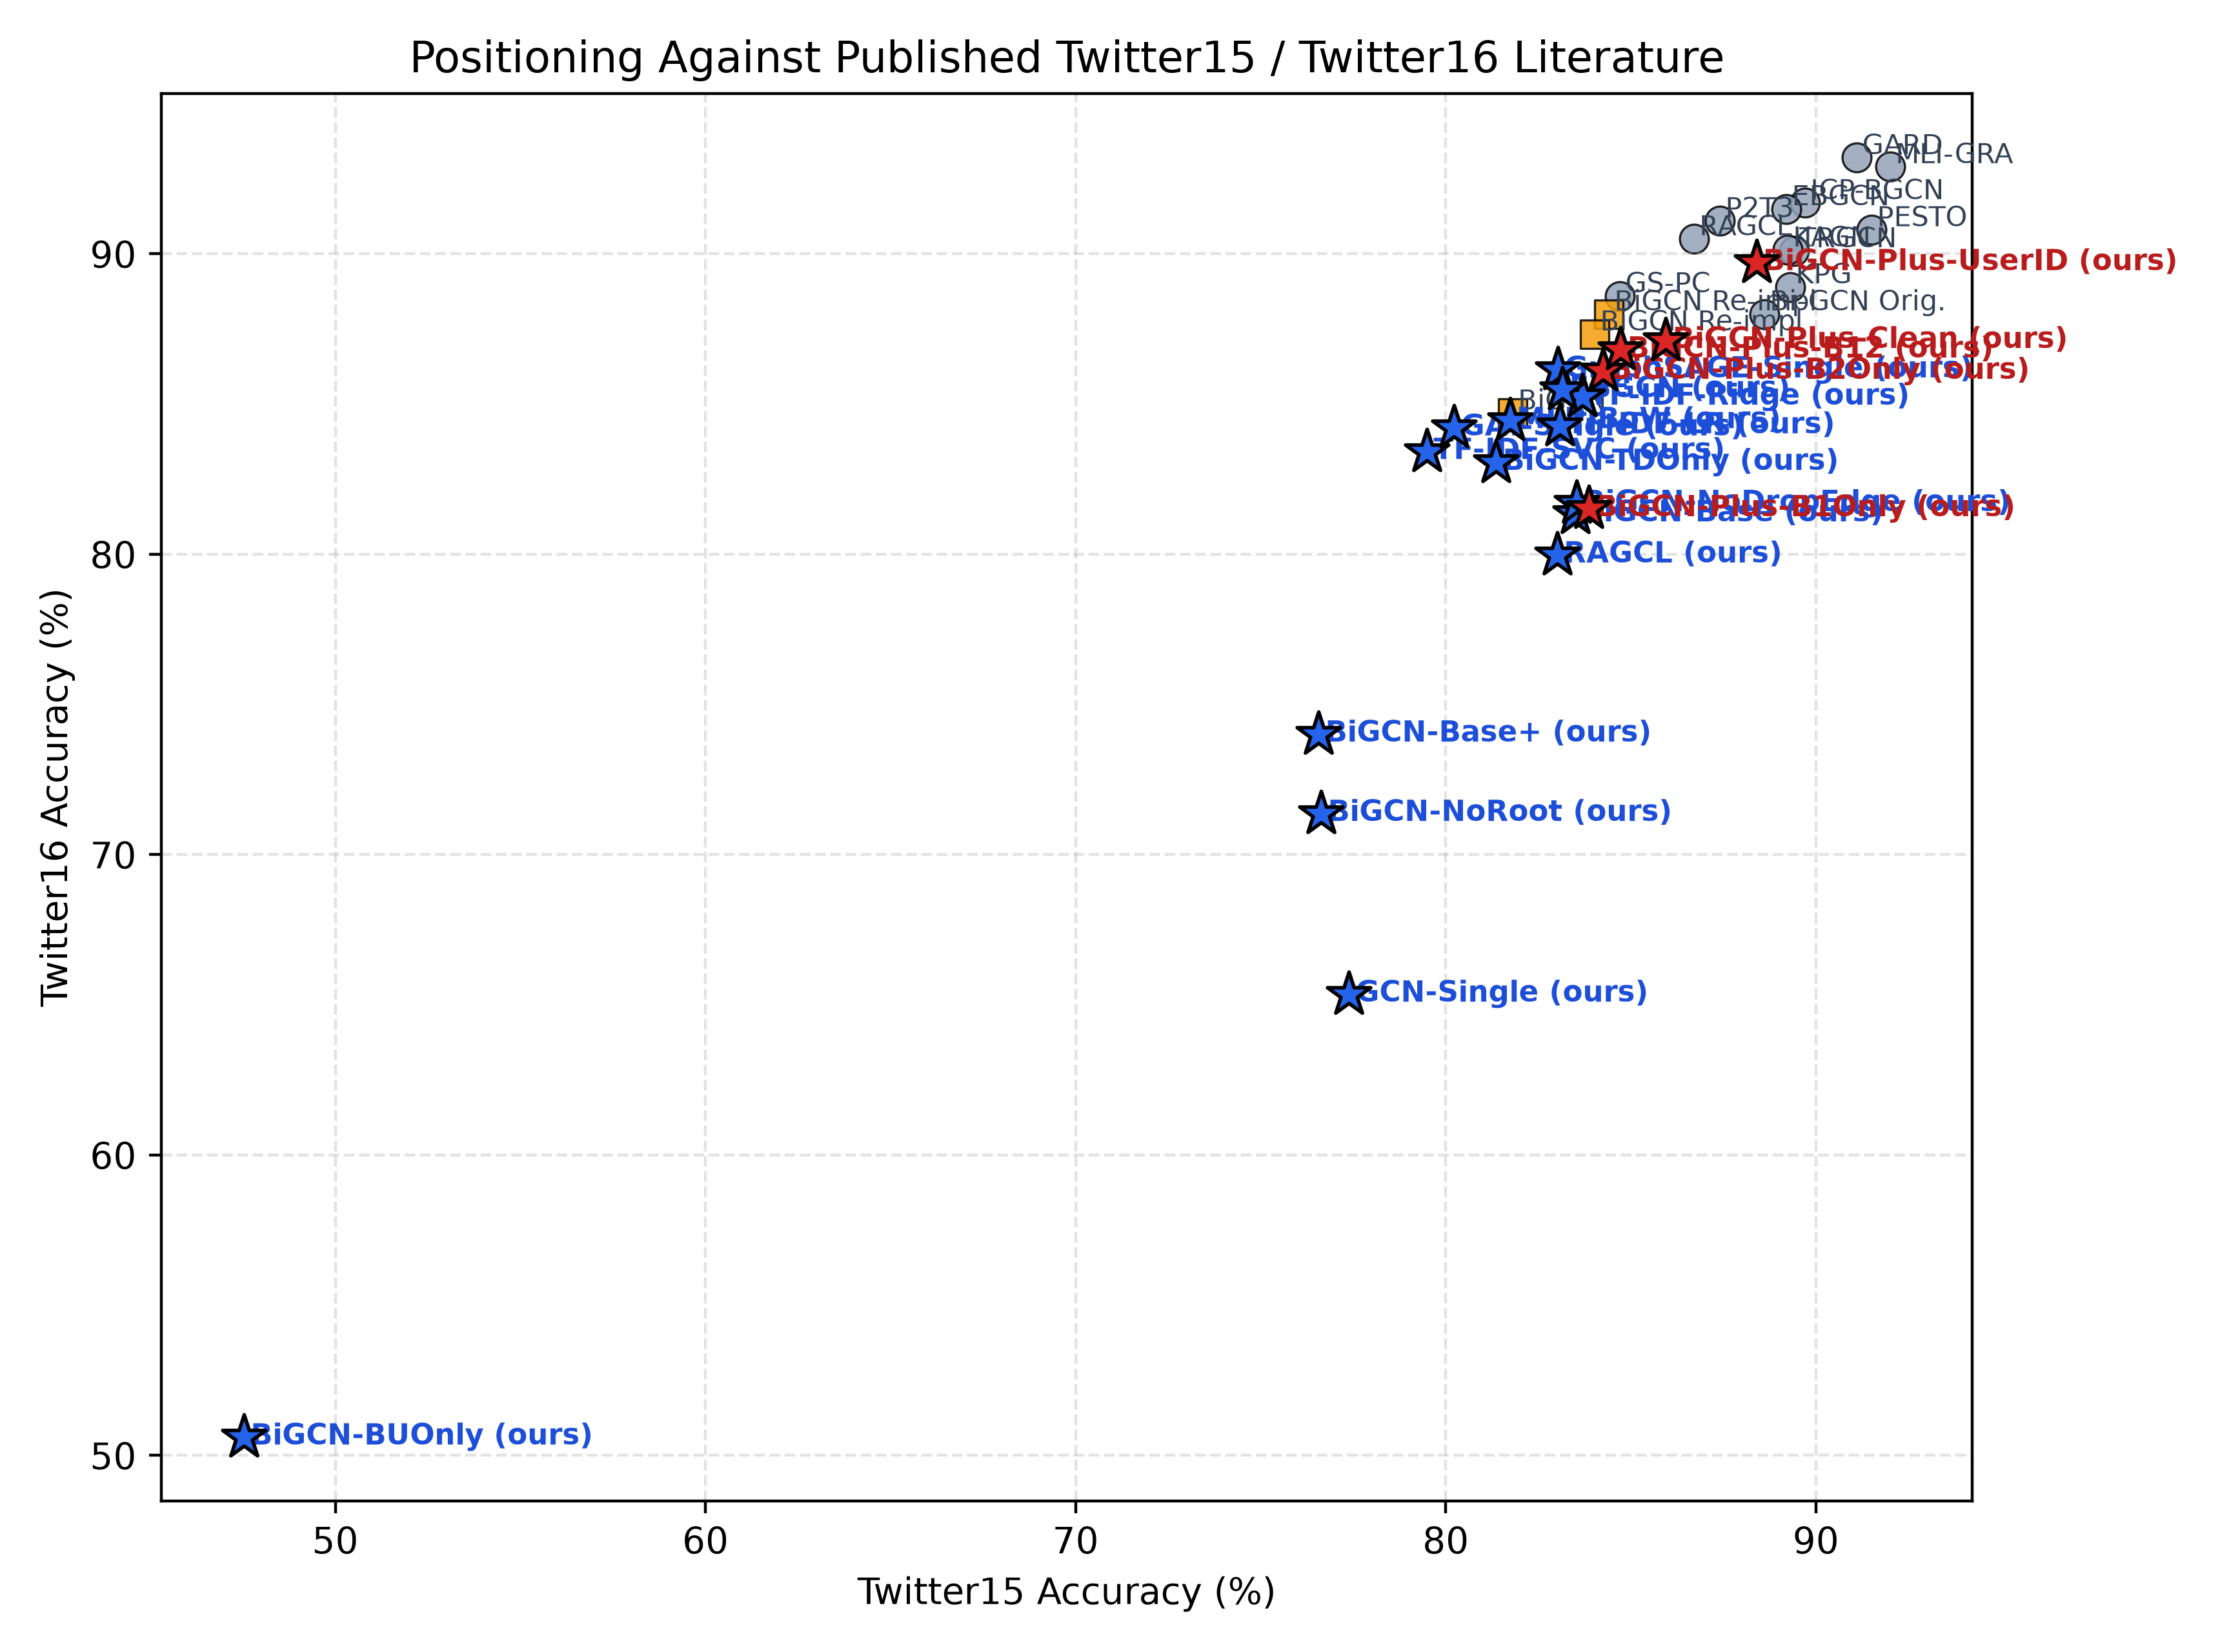
\includegraphics[width=0.76\textwidth]{figures/external_positioning.png}
    \caption[Biểu đồ định vị hiệu năng trên Twitter15 và Twitter16]{Biểu đồ phân tán định vị hiệu năng Accuracy giữa các mô hình thực nghiệm của nhóm với các công trình quốc tế công bố trên Twitter15 và Twitter16 \coderef{scripts/aggregate_results.py}{scripts/aggregate\_results.py}}
    \label{fig:external-positioning}
\end{figure}

Như thể hiện tại Bảng~\ref{tab:external-sota} và Hình~\ref{fig:external-positioning}, trong cùng điều kiện dữ liệu mở Nhóm A, mô hình chuẩn sạch \texttt{BiGCN-Plus-Clean} ($0{,}85946$ trên Twitter15; $0{,}87116$ trên Twitter16) vượt trội rõ rệt so với các bản tái lập \texttt{BiGCN} trước đây trên Twitter15 ($0{,}81800\text{--}0{,}84400$). Khi bổ sung tín hiệu tương tác tài khoản, \texttt{BiGCN-Plus-UserID} ($0{,}88389$ / $0{,}89706$) vươn lên phân khúc Khá -- Cao ngay cả khi xếp chung với Nhóm B (vượt \texttt{Bi-GCN} gốc $0{,}88000$ và \texttt{KPG} $0{,}88900$ trên Twitter16), trong khi khoảng cách $0{,}014\text{--}0{,}036$ so với nhóm đỉnh dùng \texttt{BERT + Full replies} phản ánh đúng giới hạn khách quan của việc thiếu nội dung phản bác trong các bình luận con.

\section{Phân tích chi phí tính toán và Thời gian thực thi trên GPU T4}

Toàn bộ $20$ mô hình đều được đo thời gian huấn luyện trung bình trên cùng một GPU Colab T4 (\texttt{cuda}) nhằm bảo đảm công bằng tuyệt đối. Ở nhóm cơ sở Cấp độ 1, \texttt{MLP-BoW} có tốc độ nhanh nhất ($0{,}05114\text{ s/epoch}$ trên Twitter16 và $0{,}08241\text{ s/epoch}$ trên Twitter15) nhưng bỏ qua cấu trúc đồ thị; \texttt{GraphSAGE-Single} đạt cân bằng tốt giữa tốc độ và hiệu năng ($0{,}10508\text{ s/epoch}$ trên Twitter16 và $0{,}17697\text{ s/epoch}$ trên Twitter15). Đối với nhóm Cấp độ 2, \texttt{BiGCN-Base} tiêu tốn $0{,}18385\text{ s/epoch}$ (Twitter16) và $0{,}31084\text{ s/epoch}$ (Twitter15), nhẹ hơn rõ rệt so với \texttt{RAGCL} ($0{,}44276\text{ s/epoch}$ và $0{,}74884\text{ s/epoch}$) do không phải thực hiện hai lượt tăng cường đồ thị cho mất mát tương phản. Kiến trúc đề xuất \texttt{BiGCN-Plus-Clean} chỉ tiêu tốn $0{,}23685\text{ s/epoch}$ trên Twitter16 và $0{,}39035\text{ s/epoch}$ trên Twitter15 (tức khoảng $23{,}7\text{--}39{,}0$ giây cho mỗi lượt huấn luyện $100$ epoch), chứng minh mức chi phí tính toán rất gọn nhẹ và khả thi cho triển khai thực tế.

% =====================================================================
% CHƯƠNG 5: KẾT LUẬN VÀ HƯỚNG PHÁT TRIỂN
% =====================================================================
\chapter{KẾT LUẬN VÀ HƯỚNG PHÁT TRIỂN}

\section{Tổng kết các đóng góp chính}

Đề tài đã giải quyết bài toán phát hiện tin giả và tin đồn trên mạng xã hội theo hướng kết hợp Xử lý ngôn ngữ tự nhiên và Khai phá đồ thị lan truyền với bốn đóng góp trọng tâm, toàn bộ mã nguồn và dữ liệu kiểm chứng được công khai tại kho lưu trữ \url{https://github.com/pqui-345/BiGCN-Plus-Rumor-Detection}:
\begin{enumerate}
    \item \textbf{Hệ thống hóa tập công trình khảo sát thuần Văn bản -- Đồ thị (2017--2026):} Lọc bỏ hoàn toàn nhóm nghiên cứu đa phương thức, tái cấu trúc theo $5$ nhóm phương pháp và phân nhóm theo hệ sinh thái bộ dữ liệu chuẩn, đồng thời thực hiện phân tích EDA định lượng chứng minh đặc tính lệch phải ($\text{Skewness} > 2{,}79$) và cân bằng $4$ lớp của hai bộ chuẩn Twitter15 và Twitter16.
    \item \textbf{Chuẩn hóa bộ khung thực nghiệm đa lượt chạy không rò rỉ dữ liệu:} Xây dựng quy trình thống nhất chạy lặp $5\text{ seeds} \times 5\text{ folds} = 25$ lượt/mô hình trên cùng hạ tầng GPU T4, chỉ khớp từ điển trên tập Train từng fold, ghi nhận song song hai chế độ checkpoint (\texttt{last} và \texttt{snapshot5}) kèm hệ thống $8$ nhóm độ đo và kiểm định thống kê \textit{Paired t-test}, \textit{Wilcoxon signed-rank}.
    \item \textbf{Đánh giá toàn diện hệ thống $20$ mô hình đối sánh và giải phẫu:} Thiết lập ngưỡng chuẩn cho nhóm NLP thuần văn bản (\texttt{TF-IDF-Ridge}), Cấp độ 1 (\texttt{GraphSAGE-Single}), Cấp độ 2 (\texttt{BiGCN-Base}, $4$ biến thể giải phẫu, \texttt{EBGCN}, \texttt{RAGCL}) và chứng minh vai trò thiết yếu của nhánh lan truyền xuôi cùng cơ chế tăng cường đặc trưng nút gốc.
    \item \textbf{Đề xuất kiến trúc \texttt{BiGCN-Plus} vượt trội có ý nghĩa thống kê:} Hợp nhất \texttt{Exact BiGCN}, \texttt{Dual-View GraphSAGE} không cắt cạnh và đầu \texttt{Sublinear TF-IDF} với ma trận mũ Leave-One-Out, cấu hình chuẩn sạch không phụ thuộc User-ID \texttt{BiGCN-Plus-Clean} đạt độ chính xác trung bình $\mathbf{0{,}85946}$ trên Twitter15 và $\mathbf{0{,}87116}$ trên Twitter16 (vượt mọi baseline với $p < 0{,}01$), trong khi biến thể mở rộng \texttt{BiGCN-Plus-UserID} đạt $\mathbf{0{,}88389}$ trên Twitter15 và $\mathbf{0{,}89706}$ trên Twitter16.
\end{enumerate}

\section{Hạn chế hiện tại và Hướng phát triển}

Kết quả thực nghiệm cũng chỉ ra ba giới hạn khách quan cần tiếp tục hoàn thiện trong giai đoạn nghiên cứu tiếp theo. Thứ nhất, bộ dữ liệu công khai \texttt{rumdetect2017} không lưu giữ nội dung văn bản của các bình luận phản hồi, khiến mô hình chưa khai thác được lập trường đồng tình hay phản bác (\textit{stance}) ở cấp độ từng nút con --- đây là nguyên nhân chính gây nhầm lẫn giữa lớp \textit{False Rumor} và \textit{Non-Rumor}. Thứ hai, nhóm vẫn chưa thực hiện tinh chỉnh siêu tham số tự động trên tập Validation tách riêng và chưa hoàn tất kịch bản chạy mô hình ngôn ngữ tiền huấn luyện (\texttt{RoBERTa}/\texttt{BERTweet}) kết hợp đánh giá chéo tập dữ liệu. Thứ ba, khảo sát tập công trình quốc tế cho thấy chưa có bộ dữ liệu cây lan truyền chuẩn mực nào cho tiếng Việt ($0{,}0\%$). Trong thời gian tới, nhóm định hướng tích hợp các mô hình ngôn ngữ tiền huấn luyện (như RoBERTa, PhoBERT hoặc XLM-RoBERTa) làm bộ mã hóa ngữ nghĩa cho cả bài gốc lẫn bình luận mới thu thập, đồng thời xây dựng bộ dữ liệu cây lan truyền tin giả tiếng Việt kèm kịch bản phát hiện sớm theo ngưỡng thời gian $\Delta t$.


% =====================================================================
% TÀI LIỆU THAM KHẢO (Import trực tiếp từ file ref.bib)
% =====================================================================
\newpage
\bibliographystyle{IEEEtran}
\bibliography{ref}

\end{document}